
\documentclass[11pt]{article}
\usepackage[a4paper, margin=1in]{geometry}

\usepackage{graphicx}
\usepackage{float}
\usepackage{mathtools}
\usepackage{amsfonts}
\usepackage{amssymb}
\usepackage{amsmath}
\usepackage{amsxtra}
\usepackage{array}
\usepackage{color}
\usepackage{lineno}
\usepackage{setspace}
\usepackage[usenames, dvipsnames, table]{xcolor}
\usepackage[protrusion=true, expansion=true]{microtype}
\usepackage[authoryear]{natbib}
\usepackage[font={small}, bf]{caption}
\usepackage[english]{babel}
\usepackage[T1]{fontenc}
\usepackage[utf8]{inputenc}
\usepackage{mathptmx}

\usepackage[export]{adjustbox}

\definecolor{mygray}{gray}{0.85}
\newcommand{\code}[1]{\colorbox{mygray}{\texttt{#1}}}
\newcommand{\ud}{\text{d}}
\newcommand{\ol}[1]{\overline{#1}}
\newcommand{\rem}[1]{\textcolor{red}{#1}}
\newcommand{\citeapos}[1]{\citeauthor{#1}'s (\citeyear{#1})}
\let\originalleft\left
\let\originalright\right
\renewcommand{\left}{\mathopen{}\mathclose\bgroup\originalleft}
\renewcommand{\right}{\aftergroup\egroup\originalright}
\newcommand*{\logten}{\mathop{\log_{10}}}    
\renewcommand\thefigure{S\arabic{figure}}
\renewcommand\thetable{S\arabic{table}}
\renewcommand\thesection{S\arabic{section}}
\renewcommand\theequation{S\arabic{equation}}

\clubpenalty = 10000
\widowpenalty = 10000
\bibpunct{(}{)}{,}{a}{}{,}
\DeclareMathAlphabet{\mathcal}{OMS}{txsy}{m}{n}
\allowdisplaybreaks
\graphicspath{{../../SI/}}


\title{A Bayesian network approach to trophic metacommunities\\shows habitat loss accelerates top species extinctions\\ \medskip Supporting Information}
\author{Johanna H\"aussler, Gy\"orgy Barab\'as \& Anna Ekl\"of}
\date{}


\begin{document}

\maketitle


\section{Bayesian Networks} 
\label{sec:BN}

A Bayesian network is a graphical model for the probabilistic relationships among a set of variables \citep{Jensen1996, Eklofetal2013MEE}. In the context of food webs, the probability of each species going extinct is a function of the probabilities of its resources going extinct.

More specifically, a species $C$ has, first of all, a baseline probability of extinction $\pi_C$; the species goes extinct with this likelihood even if it has full access to its resources. Such a baseline extinction probability may be related, for instance, to the fact that individual habitat patches are small in size, supporting only a few individuals and therefore prone to extinction via demographic stochasticity. Second, if the species has access to only a subset of its resources, its extinction probability increases, reaching $1$ when all resources are absent.

Let species $C$ have two prey items, $A$ and $B$ (the results below are straightforwardly generalizable to an arbitrary number of prey), and assume that the conditional probabilities of species $C$ being absent given the presence or absence of its prey items are known: $P(\neg C|A B)$ is the probability that $C$ is extinct given that both its prey are present; $P(\neg C|\neg A B)$ is the probability that $C$ is extinct given that prey $A$ is absent but prey $B$ is present; and so on. To obtain the marginal probability $P(\neg C)$ of $C$ going extinct, we use the law of total probability:
\begin{equation}
  \label{eq:BN_marginal_example}
  \begin{split}
    P(\neg C) &= P(\neg C|A B)P(A)P(B) + P(\neg C|\neg A B)P(\neg A)P(B)
    \\ &\quad + P(\neg C|A \neg B)P(A)P(\neg B) + P(\neg C|\neg A \neg B)
    P(\neg A)P(\neg B) \ .
  \end{split}
\end{equation}
In principle, the conditional probabilities may be as complicated as demanded by the natural history of the modeled ecological scenario. For instance, it is possible to have $P(\neg C|A B) > P(\neg C| \neg A B)$, with the probability of extinction greater in the presence of two alternative prey items than with only one. For example, if species $A$ and $B$ are mutualists (for example, $A$ emits an alarm call when a predator is present, alerting members of both $A$ and $B$), then the absence of $A$ may in fact make predation easier for $C$.

Here, however, we operate with the simple assumption that the conditional probabilities of species $C$ going extinct depend only on the fraction $f$ of its resources lost. (We relax this assumption later, in Section~\ref{sec:weighted}.) We model this conditional probability as
\begin{equation}
  \label{eq:BN_prob}
  P(\neg C|f) = \pi_C + (1 - \pi_C) w(f) \ ,
\end{equation}
where the weighting function $w(f)$ is monotonically increasing and defined for $0 \le f \le 1$, such that $w(0)=0$ and $w(1)=1$. The former condition holds when all resources are present, in which case Eq.~\ref{eq:BN_prob} yields $P(\neg C|0) = \pi_C$, the baseline extinction probability. The latter condition means that when all resources are lost, $P(\neg C|1) = 1$: no species can survive without any resources sustaining it.

To see how this is applied, let us assume both $A$ and $B$ are basal species. We then have $P(\neg A) = 1 - P(A) = \pi_A$, and the same for species $B$. Using Eq.~\ref{eq:BN_prob} in Eq.~\ref{eq:BN_marginal_example}:
\begin{equation}
  \label{eq:BN_marginal_example_2}
  \begin{split}
    P(\neg C) &= [\pi_C + (1 - \pi_C) w(0)] (1 - \pi_A) (1 - \pi_B) +
    [\pi_C + (1 - \pi_C) w(1/2)] \pi_A (1 - \pi_B) \\ &\quad +
    [\pi_C + (1 - \pi_C) w(1/2)] (1 - \pi_A) \pi_B +
    [\pi_C + (1 - \pi_C) w(1)] \pi_A \pi_B \ .
  \end{split}
\end{equation}
To make further progress, one must specify the form of $w(f)$. For instance, if $w(f)=f$, then
\begin{equation}
  \label{eq:BN_marginal_example_3}
  P(\neg C) = \pi_C (1 - \pi_A) (1 - \pi_B) +
  \left( \frac{1 + \pi_C}{2} \right) \pi_A (1 - \pi_B) +
  \left( \frac{1 + \pi_C}{2} \right) (1 - \pi_A) \pi_B + \pi_A \pi_B \ .
\end{equation}
For example, if $\pi_A = \pi_B = \pi_C = 0.1$, then Eq.~\ref{eq:BN_marginal_example_3} gives $P(\neg C) = 0.19$ (and $P(C) = 1-P(\neg C) = 0.81$). The marginal probability of extinction can be calculated analogously for any species with any number of resource items. However, when the resource species are not basal, one should use the (already calculated) marginal persistence and extinction probabilities of the prey in Eq.~\ref{eq:BN_marginal_example}. Thus, determining the extinction probabilities of all species is a bottom-up calculation process: we start with basal species, then move on to species only consuming those basal species, and so on, to the very top of the food web.

This also means that the Bayesian network approach has two important limitations. First, the food webs must be acyclic, as otherwise this bottom-up approach would not work. Second, top-down effects cannot be implemented, since the loss of the top predator from the system has no effect on the persistence probabilities of species at lower trophic levels.


\section{The trophic metacommunity model} \label{sec:tmm}

We generalize single-species metapopulation models on fragmented landscapes \citep{HanskiOvaskainen2000, OvaskainenHanski2001, HanskiOvaskainen2003, Grillietal2015} to trophic communities. Let $S$ be the number of species, $N$ the number of habitat patches, and $p_i^k$ the probability that species $i$ is found in patch $k$. The basic model reads
\begin{equation}
  \label{eq:model}
  \frac{\ud p_i^k}{\ud t} = (1 - p_i^k) C_i^k - p_i^k E_i^k \ ,
\end{equation}
where $C_i^k$ and $E_i^k$ are the colonization and extinction rates of species $i$ in patch $k$; both may depend on the patch occupancies $p_i^k$. Here and elsewhere we follow the convention that subscripts denote species indices and superscripts denote patch indices.

For our trophic metacommunity approach, we model colonization using a species-dependent landscape matrix:
\begin{equation}
  \label{eq:colonization}
  C_i^k = \sum_{l=1}^N M_i^{kl} p_i^l
\end{equation}
\citep{OvaskainenHanski2001}, where $M_i^{kl}$, the $(k,l)$th entry of species $i$'s landscape matrix, is the rate of dispersal of species $i$ from patch $l$ to $k$. In turn, the extinction rates are modeled based on the probability of extinction $\delta_i^k$ of species $i$ in patch $k$ per unit time. To convert this probability into the rate $E_i^k$, we treat extinction as a Poisson process. This is justified on the grounds that metapopulation approaches assume a time scale separation between migration and local population dynamics, with the former being much slower than the latter \citep{Hanski1994}. This allows one to treat populations in local patches as being in population dynamical quasi-equilibrium. In this quasi-equilibrium state, there is some constant probability of going extinct per unit of time in each patch, leading to the Poisson process with rate parameter $E_i^k$:
\begin{equation}
  \label{eq:probrate}
  \delta_i^k = 1 - \exp(-E_i^k) \ .
\end{equation}
This yields an extinction probability of $0$ when $E_i^k$ is zero, and a probability of one for $E_i^k$ infinitely large. Solving for the rate, we get
\begin{equation}
  \label{eq:extinction}
  E_i^k = -\log(1 - \delta_i^k) \ .
\end{equation}

The essence of our approach to trophic metacommunities is the way we model the extinction probabilities $\delta_i^k$. These are calculated from a Bayesian network representation of the food web. Given baseline extinction probabilities $\pi_i^k$ for species $i$ in patch $k$, we equate $\delta_i^k$ with the marginal probability of extinction in patch $k$, calculated from the Bayesian network. Since $\delta_i^k$ is the probability of extinction per unit time (during which no colonization events happen due to the time scale separation between local dynamics and dispersal mentioned above), the probability of a species being present in a given patch $k$ is the product of two probabilities: the local probability $P^k(i) = 1 - P^k(\neg i)$ of persistence from the Bayesian network, multiplied by the probability that species $i$ is present in patch $k$ in the first place. This latter probability is by definition the patch occupancy $p_i^k$, and so, when applying Eq.~\ref{eq:BN_marginal_example} to obtain the extinction probability of a species $i$, we perform the
\begin{equation}
  \label{eq:bayesprob}
  1-P^k(\neg \text{prey}) \rightarrow (1-P^k(\neg \text{prey})) p_\text{prey}^k
\end{equation}
replacement (see Section~\ref{sec:anal} for example applications).

For basal species, we assume that the nutrients they use are always available. This leads to $p_j^k = 1$ in all patches for all nutrients $j$, so for basals, $\delta_{\text{basal}}^k = 1 - (1 - \pi_\text{basal}^k)p_j^k = \pi_\text{basal}^k$.


\section{Simple model properties} \label{sec:simpleprops}

For a single focal species, Eq.~\ref{eq:model} belongs in the class of spatially realistic Levins models in which there is a single measure of the metapopulation capacity, defined as the leading eigenvalue of $\partial g_i^k / \partial p_i^l$ evaluated at $p_i^k = 0$ \citep{OvaskainenHanski2001}, where $g_i^k = C_i^k / E_i^k$ is the model's principal map. Using Eqs.~\ref{eq:colonization} and \ref{eq:extinction}, the principal map reads
\begin{equation}
  \label{eq:principalmap}
  g_i^k = -\frac{1}{\log(1 - \delta_i^k)} \sum_{l=1}^N M_i^{kl} p_i^l \ .
\end{equation}
Due to our Bayesian network approach, the extinction likelihood $\delta_i^k$ is a function of the patch occupancies of the focal species' prey, but not those of the focal species itself. That is, $\delta_i^k$ is independent of $p_i^k$. The Jacobian of the principal map evaluated at $p_i^k = 0$, which we will denote by $A_i^{kl}$, therefore simply reads
\begin{equation}
  \label{eq:pmjac}
  A_i^{kl} = \left. \frac{\partial g_i^k}{\partial p_i^l} \right|_{p_i^k=0} =
  -\frac{M_i^{kl}}{\log(1 - \delta_i^k)} \ .
\end{equation}
The metapopulation capacity $\lambda_i$ of species $i$ is the leading eigenvalue of this matrix. If $\lambda_i$ exceeds $1$, the metapopulation persists at equilibrium, otherwise all $p_i^k$ are zero.

To obtain the equilibrium patch occupancies, we set $\ud p_i^k / \ud t = 0$ in Eq.~\ref{eq:model}. The equilibrial patch occupancy distribution is then expressed as $C_i^k/(C_i^k + E_i^k) = g_i^k / (g_i^k + 1)$. Defining the map
\begin{equation}
  \label{eq:itermap}
  h_i^k = \frac{g_i^k}{g_i^k + 1} \ ,
\end{equation}
the equilibrial $p_i^k$ can be obtained by iterating this map until its fixed point is reached. In spatially realistic Levins-type models like Eq.~\ref{eq:model}, the equilibrium state is unique and stable with respect to this iteration scheme \citep{OvaskainenHanski2001}. This means that the iteration eventually converges to the true equilibrium values for any valid nonzero starting condition, yielding an efficient numerical method for finding the equilibrium patch occupancies.

The value of a given habitat patch $k$ to a metapopulation $i$ is defined as $V_i^k = (\lambda_i - \lambda_i^{-k}) / \lambda_i$, where $\lambda_i^{-k}$ denotes species $i$'s  metapopulation capacity after removing patch $k$. For models like Eq.~\ref{eq:model}, this relative decrease can be obtained as
\begin{equation}
  \label{eq:Vik}
  V_i^k = \frac{v_i^k w_i^k}{\sum_{l=1}^N v_i^l w_i^l} \ ,
\end{equation}
where $v_i^k$ is the left and $w_i^k$ the right eigenvector belonging to the leading eigenvalue giving the metapopulation capacity \citep{OvaskainenHanski2001}. Patches can be ranked using this formula, from most to least important for persistence (the most important causing the largest relative decline in the metapopulation capacity, and vice versa). This ranking is local in the sense that it is not preserved after removing a patch: after removal, the patch values must be recalculated using Eq.~\ref{eq:Vik}. In practice, removing a small fraction of patches will only alter the rankings by a small amount, so this recalculation needs not to happen after the removal of every single patch.

The average patch occupancy at equilibrium, $\ol{p}_i$, can be approximated as
\begin{equation}
  \label{eq:papprox}
  \ol{p}_i \approx 1 - \frac{1}{\lambda_i} \ ,
\end{equation}
where $\lambda_i$ is the metapopulation capacity for species $i$ (the leading eigenvalue of $A_i^{kl}$ in Eq.~\ref{eq:pmjac}). Formally, this approximation works best for the weighted average
\begin{equation}
  \label{eq:weighted}
  \ol{p}_i = \sum_{k=1}^N p_i^k V_i^k
\end{equation}
\citep{OvaskainenHanski2001}. However, Eq.~\ref{eq:papprox} works acceptably even for the simple average $\ol{p}_i = \sum_{k=1}^N p_i^k / N$.


\section{Analytically tractable trophic networks} \label{sec:anal}

\subsection{One consumer, one resource} \label{sec:CR}

The simplest example of a trophic metacommunity consist of just two species: one consumer $C$ and one basal resource $R$. Below we analyze the trophic metacommunity formed by these species, step by step.

\textit{\textbf{Step 1: Solve for the extinction probabilities using the Bayesian network approach.}}
The baseline probabilities of extinction for the resource and the consumer are $\pi_R^k$ and $\pi_C^k$, respectively. Since $R$ is a basal species, we have $P^k(\neg R) = \pi_R^k$. The resource's probability of extinction in a patch with resource occupancy $p_R^k$ is written using Eq.~\ref{eq:bayesprob}: $\delta_R^k = 1- (1 - P^k(\neg R)) p_R^k = 1 - (1 - \pi_R^k) p_R^k$. We now obtain the consumer's marginal probability of extinction $\delta_C^k$ in the style of Eq.~\ref{eq:BN_marginal_example}, except with only a single resource and applying Eq.~\ref{eq:bayesprob}:
\begin{equation}
  \label{eq:BN_marginal_CR}
  \begin{split}
    \delta_C^k &= P^k(\neg C|R) P^k(R) + P^k(\neg C|\neg R) P^k(\neg R)
    \\ &= P^k(\neg C|R) (1 - \pi_R^k) p_R^k + P^k(\neg C|\neg R)
    [ 1 - (1 - \pi_R^k) p_R^k ] \ .
  \end{split}
\end{equation}
Using Eq.~\ref{eq:BN_prob} to write the conditional probabilities, and noting that $w(0)=0$ and $w(1)=1$ regardless of the form of $w(f)$, we get $P^k(\neg C|R) = \pi_C^k$ and $P^k(\neg C|\neg R) = 1$:
\begin{equation}
  \label{eq:BN_marginal_CR_2}
  \delta_C^k = \pi_C^k (1 - \pi_R^k) p_R^k + 1 - (1 - \pi_R^k) p_R^k \ .
\end{equation}
Rearranging, and writing out the marginal extinction probabilities of both species:
\begin{align}
  \label{eq:BN_marginal_CR_R_detailed}
  \delta_R^k &= \pi_R^k \ , \\
  \label{eq:BN_marginal_CR_C_detailed}
  \delta_C^k &= 1 - (1 - \pi_C^k) (1 - \pi_R^k) p_R^k \ .
\end{align}

\textit{\textbf{Step 2: Obtain the metapopulation capacity of each species.}}
We first calculate the Jacobian matrix of each species' principal map evaluated at zero. Substituting Eqs.~\ref{eq:BN_marginal_CR_R_detailed} and \ref{eq:BN_marginal_CR_C_detailed} into Eq.~\ref{eq:pmjac}:
\begin{align}
  \label{eq:BN_A_CR_R}
  A_R^{kl} &= -\frac{M_R^{kl}}{\log(1 - \pi_R^k)} \ , \\
  \label{eq:BN_A_CR_C}
  A_C^{kl} &= -\frac{M_C^{kl}}{\log[(1 - \pi_C^k) (1 - \pi_R^k) p_R^k]} \ .
\end{align}
The metapopulation capacities are given by the leading eigenvalues $\lambda_R$ and $\lambda_C$ of $A_R^{kl}$ and $A_C^{kl}$, respectively. For persistence, they must exceed $1$. To evaluate $\lambda_C$, one must know $p_R^k$ beforehand---this can be obtained e.g.\ by iterating Eq.~\ref{eq:itermap} for the basal species.

\textit{\textbf{Step 3: Approximate metapopulation capacities analytically.}}
In general, to get a meaningful non-numerical answer for the metapopulation capacities, we must simplify the problem. This can be done in two steps:

\textit{Step 3a: Replace quantities with their averages.}
This is done by performing the $\pi_i^k \rightarrow \pi_i$, $p_i^k \rightarrow \ol{p}_i$ substitutions in the expressions for the $A_i^{kl}$. Eqs.~\ref{eq:BN_A_CR_R} and \ref{eq:BN_A_CR_C} then read
\begin{align}
  \label{eq:BN_A_CR_R_nonspatial}
  A_R^{kl} &\approx -\frac{M_R^{kl}}{\log(1 - \pi_R)} \ , \\
  \label{eq:BN_A_CR_C-nonspatial}
  A_C^{kl} &\approx -\frac{M_C^{kl}}{\log[(1 - \pi_C) (1 - \pi_R) \ol{p}_R]} \ .
\end{align}
The denominators are now simply numbers. The eigenvalues of $A_R^{kl}$ and $A_C^{kl}$ are thus the eigenvalues of the landscape matrices, divided by these numerical factors:
\begin{align}
  \label{eq:BN_lambda_R_nonspatial}
  \lambda_R &\approx -\frac{\lambda_{M_R}}{\log(1-\pi_R)} \ , \\
  \label{eq:BN_lambda_C_nonspatial}
  \lambda_C &\approx -\frac{\lambda_{M_C}}{\log[(1-\pi_C) (1-\pi_R)\ol{p}_R]} \ ,
\end{align}
where $\lambda_{M_i}$ is the leading eigenvalue of the landscape matrix of species $i$.

\textit{Step 3b: Approximate the average patch occupancies using Eq.~\ref{eq:papprox}.}
In our example, we have $\ol{p}_R \approx 1 - 1 / \lambda_R$:
\begin{align}
  \label{eq:BN_lambda_R_nonspatial_2}
  \lambda_R &\approx -\frac{\lambda_{M_R}}{\log(1 - \pi_R)} \ , \\
  \label{eq:BN_lambda_C_nonspatial_2}
  \lambda_C &\approx -\frac{\lambda_{M_C}}{\log\left[ (1 - \pi_C) (1 - \pi_R)
              \left( 1 + \dfrac{\log(1 - \pi_R)}{\lambda_{M_R}}\right)\right]} \ .
\end{align}
Figure~\ref{fig:CR_persist} visualizes these persistence conditions.

\begin{figure}[!ht]
  \centering
  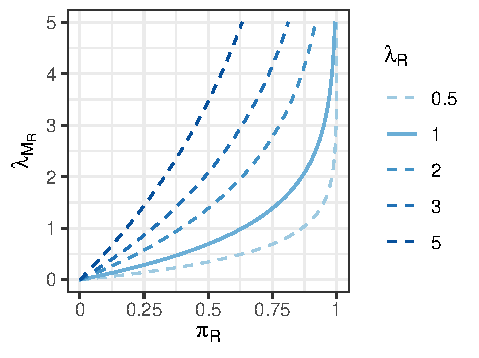
\includegraphics[width=0.49\textwidth]{R_persist.pdf}
  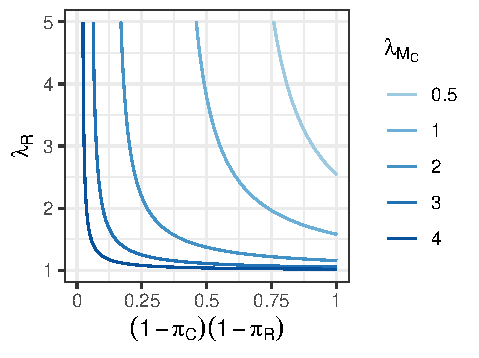
\includegraphics[width=0.49\textwidth]{C_persist.pdf}
  \caption{Persistence in the one consumer, one resource system. Left: curves of identical resource metapopulation capacities $\lambda_R$ (colors), as a function of the resource's baseline extinction probability $\pi_R$ (abscissa) and the leading eigenvalue of its landscape matrix $\lambda_{M_R}$ (ordinate). The solid line corresponds to a metapopulation capacity of one; the species persists for combinations of $\pi_R$ and $\lambda_{M_R}$ falling above this line on the graph, and goes extinct below this line. Right: curves along which the consumer metapopulation capacity, $\lambda_C$, is equal to one, for various values of the leading eigenvalue of its landscape matrix $\lambda_{M_C}$ (colors), the product of the consumer and resource baseline persistence probabilities (abscissa), and the resource metapopulation capacity $\lambda_R$ (ordinate). For each value of $\lambda_{M_C}$, points above the corresponding line on the graph lead to the consumer's persistence.}
  \label{fig:CR_persist}
\end{figure}

\subsection{Food chain} \label{sec:chain}

The above can be generalized to trophic chains of arbitrary length. Let there be $S$ species with baseline extinction probabilities $\pi_i^k$. Species $1$ is basal and is eaten by species $2$; species $S$ is a top predator eating species $S-1$; and species $1 < i < S$ eat species $i-1$ and are eaten by species $i+1$.

\textit{\textbf{Step 1: Solve for the extinction probabilities using the Bayesian network approach.}}
The probability of species $i+1$ being extinct can be written as
\begin{equation}
  \label{eq:BN_marginal_chain}
  \delta_{i+1}^k = P^k(\neg (i+1)|i) P^k(i) +
  P^k(\neg (i+1)|\neg i) P^k(\neg i) \ .
\end{equation}
Since every species $i>1$ has exactly one prey, from Eq.~\ref{eq:BN_prob} we can write $P^k(\neg (i+1)|i) = \pi_{i+1}^k$ and $P^k(\neg (i+1)|\neg i) = 1$:
\begin{equation}
  \label{eq:BN_marginal_chain_2}
  \delta_{i+1}^k = \pi_{i+1}^k P^k(i) + P^k(\neg i) \ .
\end{equation}
Using Eq.~\ref{eq:bayesprob}, we have
\begin{equation}
  \label{eq:BN_marginal_chain_3}
  \begin{split}
    \delta_{i+1}^k &= \pi_{i+1}^k (1-\delta_i^k)p_i^k + 1 - (1 - \delta_i^k)
    p_{i-1}^k \\ &= 1 - (1-\pi_{i+1}^k) p_i^k (1 - \delta_i^k) \ ,
  \end{split}
\end{equation}
which is a recursion equation for the $\delta_i^k$ with initial condition $\delta_1^k = \pi_1^k$. The recursion can be solved explicitly:
\begin{equation}
  \label{eq:BN_marginal_chain_4}
  \delta_i^k = 1 - (1 - \pi_i^k) \prod_{n=1}^{i-1} (1 - \pi_n^k) p_n^k \ .
\end{equation}
That this is indeed the solution is shown by writing Eq.~\ref{eq:BN_marginal_chain_4} for $i+1$:
\begin{equation}
  \label{eq:BN_marginal_chain_5}
  \begin{split}
    \delta_{i+1}^k &= 1 - (1 - \pi_{i+1}^k) \prod_{n=1}^{i} (1 - \pi_n^k) p_n^k
    \\ &= 1 - (1-\pi_{i+1}^k) p_i^k \underbrace{(1-\pi_i^k) \prod_{n=1}^{i-1}
      (1 - \pi_n^k) p_n^k}_{1 - \delta_i^k
      \text{ (Eq.~\ref{eq:BN_marginal_chain_4})}} \\ &=
    1 - (1-\pi_{i+1}^k) p_i^k (1 - \delta_i^k) \ ,
  \end{split}
\end{equation}
recovering Eq.~\ref{eq:BN_marginal_chain_3}.

For instance, applying Eq.~\ref{eq:BN_marginal_chain_4} to a tritrophic chain with a resource ($R$), consumer ($C$), and top ($T$) species, we get
\begin{align}
  \label{eq:BN_marginal_chain_R}
  \delta_R^k &= \pi_R^k \ , \\
  \label{eq:BN_marginal_chain_C}
  \delta_C^k &= 1 - (1 - \pi_C^k) (1 - \pi_R^k) p_R^k \ , \\
  \label{eq:BN_marginal_chain_T}
  \delta_T^k &= 1 - (1 - \pi_T^k) (1 - \pi_C^k) (1 - \pi_R^k) p_R^k p_C^k \ .
\end{align}

\textit{\textbf{Step 2: Obtain the metapopulation capacity of each species.}}
We first calculate the Jacobian matrix of each species' principal map evaluated at zero, from Eq.~\ref{eq:pmjac}. Using Eq.~\ref{eq:BN_marginal_chain_5}, we get
\begin{equation}
  \label{eq:BN_A_chain}
  A_i^{kl} = -\frac{M_i^{kl}}{\log\left[ (1 - \pi_i^k) \prod_{n=1}^{i-1}
      (1 - \pi_n^k) p_n^k \right]}
\end{equation}
for $i>1$, and $A_1^{kl} = -M_1^{kl} / \log(1 - \pi_i^k)$ for the basal species. The metapopulation capacities are the leading eigenvalues $\lambda_i$ of the matrices $A_i^{kl}$. They can be computed sequentially, starting from the basal species and moving up the chain. For each species, we obtain its equilibrium patch occupancy distribution $p_i^k$, for example from Eq.~\ref{eq:itermap}. We then use these to compute $A_i^{kl}$ and then $\lambda_i$ for subsequent species.

\textit{\textbf{Step 3: Approximate metapopulation capacities analytically.}}
Using the nonspatial baseline extinction probabilities (\textit{Step 3a}), we rewrite Eq.~\ref{eq:BN_A_chain} as
\begin{equation}
  \label{eq:BN_A_chain_2}
  A_i^{kl} \approx -\frac{M_i^{kl}}{\log\left[ (1 - \pi_i) \prod_{n=1}^{i-1}
      (1 - \pi_n) \ol{p}_n \right]} \ .
\end{equation}
If $\lambda_{M_i}$ is the leading eigenvalue of species $i$'s landscape matrix $M_i^{kl}$, then
\begin{equation}
  \label{eq:BN_lambda_chain}
  \lambda_i \approx -\frac{\lambda_{M_i}}{\log\left[ (1 - \pi_i) \prod_{n=1}^{i-1}
      (1 - \pi_n) \ol{p}_n \right]} \ .
\end{equation}
We can now use Eq.~\ref{eq:papprox} to express the average patch occupancies (\textit{Step 3b}):
\begin{equation}
  \label{eq:BN_lambda_chain_2}
  \lambda_i \approx -\frac{\lambda_{M_i}}{\log\left[ (1 - \pi_i) \prod_{n=1}^{i-1}
      (1 - \pi_n) \left( 1 - 1/\lambda_n \right) \right]} \ .
\end{equation}
For $\lambda_{i+1}$, this reads
\begin{equation}
  \label{eq:BN_lambda_chain_3}
  \begin{split}
    \lambda_{i+1} &\approx - \frac{\lambda_{M_{i+1}}}{\log\left[ (1 - \pi_{i+1})
        \prod_{n=1}^{i} (1 - \pi_n) \left( 1 - 1/\lambda_n \right) \right]}
    \\ &= - \frac{\lambda_{M_{i+1}}}{\log \left[ (1 - \pi_{i+1}) (1-1/\lambda_i)
        (1 - \pi_i) \prod_{n=1}^{i-1} (1 - \pi_n) \left( 1-1/\lambda_n
        \right) \right]}
    \\ &= - \frac{\lambda_{M_{i+1}}}{\log \left[ (1 - \pi_{i+1}) (1-1/\lambda_i)
      \right] + \log \left[(1 - \pi_i) \prod_{n=1}^{i-1} (1 - \pi_n)
          \left( 1-1/\lambda_n \right) \right]} \ .
  \end{split}
\end{equation}
The last term in the denominator is $-\lambda_{M_i}/\lambda_i$ by Eq.~\ref{eq:BN_lambda_chain_2}, therefore
\begin{equation}
  \label{eq:BN_lambda_chain_4}
  \lambda_{i+1} \approx - \frac{\lambda_{M_{i+1}}}{\log \left[ (1 - \pi_{i+1})
      (1-1/\lambda_i) \right] - \lambda_{M_i} / \lambda_i} \ ,
\end{equation}
and $\lambda_1 = -\lambda_{M_1} / \log(1-\pi_1)$ for the basal species, giving a recursion equation for the metapopulation capacities $\lambda_i$. In fact, one can formally say $\lambda_0 = \infty$ (substituting this into Eq.~\ref{eq:BN_lambda_chain_4} returns the correct $\lambda_1$), which biologically translates into our assumption that the resources of basal species (such as light, water, and nutrients) are always available regardless of landscape fragmentation.

To simplify Eq.~\ref{eq:BN_lambda_chain_4} further, let us assume that the baseline probability of extinction is the same at all trophic levels: $\pi_i \equiv \pi$ for all species. Let us also assume that the landscape matrices of the species are identical: $\lambda_{M_i} \equiv \lambda_M$. Eq.~\ref{eq:BN_lambda_chain_4} then becomes
\begin{equation}
  \label{eq:BN_lambda_chain_5}
  \lambda_{i+1} \approx \frac{\lambda_M}{\lambda_M / \lambda_i -\log \left[ (1 -
      \pi) (1-1/\lambda_i) \right]} \ ,
\end{equation}
with $\lambda_0 = \infty$. The recursion is only meaningful until $\lambda_i$ drops below $1$, meaning that the $i$th trophic level cannot persist. To put the equation in an even more convenient form, we divide both sides by $\lambda_M$ and then take reciprocals:
\begin{equation}
  \label{eq:BN_lambda_chain_invert}
  \frac{\lambda_M}{\lambda_{i+1}} = \frac{\lambda_M}{\lambda_i} -
  \log \left[ (1 - \pi) \left( 1 - \frac{1}{\lambda_i} \right) \right] \ .
\end{equation}
Subtracting $\lambda_M/\lambda_i$ from both sides, and introducing the notations $\Lambda_i = 1/\lambda_i$ and $\Lambda_M = 1/\lambda_M$:
\begin{equation}
  \label{eq:BN_Lambda_chain}
  \frac{\Lambda_{i+1} - \Lambda_i}{\Lambda_M} =
  - \log \left[ (1 - \pi) (1 - \Lambda_i) \right] \ .
\end{equation}
Since $\Lambda_i = 1/\lambda_i$ and $\lambda_0 = \infty$, the initial condition for this recursion equation is $\Lambda_0 = 0$; now persistence requires $\Lambda_i$ to be less than one, and the recursion is only meaningful until $\Lambda_i$ exceeds $1$.

We now show that the sequence of inverse metapopulation capacities $\Lambda_i$ defined by Eq.~\ref{eq:BN_Lambda_chain} is strictly increasing, and it is guaranteed to go above the persistence threshold of $1$ at some point (as long as the baseline extinction probability $\pi$ is not exactly zero, in which case trophic chains of arbitrary length will trivially be able to persist). Indeed, the right hand side of Eq.~\ref{eq:BN_Lambda_chain}, measuring the scaled difference between the $\Lambda$'s of two adjacent trophic levels, is strictly positive: since $(1-\pi)$ is between $0$ and $1$, and so is $(1-\Lambda_i)$ (because $\Lambda_0 = 0$, and persistence requires $\Lambda_i < 1$), their product is also a number between $0$ and $1$. The negative log of such a number is a positive number: $-\log[(1-\pi)(1-\Lambda_i)] > 0$. Furthermore, Eq.~\ref{eq:BN_Lambda_chain} has no biologically meaningful (positive) fixed point, and therefore the fact that $\Lambda_i$ increases at every step means it must eventually increase above the persistence threshold of $1$. The fixed point $\Lambda^*$ of \ref{eq:BN_Lambda_chain} is obtained by setting $\Lambda_{i+1} = \Lambda_i = \Lambda^*$:
\begin{equation}
  \label{eq:BN_Lambda_chain_fp}
  0 = - \log \left[ (1 - \pi) (1-\Lambda^*) \right] \ ,
\end{equation}
whose unique solution is manifestly negative:
\begin{equation}
  \label{eq:BN_Lambda_chain_fp_sol}
  \Lambda^* = - \frac{\pi}{1 - \pi} < 0
\end{equation}
and therefore lies outside the biologically relevant positive domain.

The fact that the $\Lambda_i$ must eventually increase above the persistence threshold of $1$ imposes a cap on the maximum number of trophic levels. To explore how restrictive this cap is, we consider the limit of a very small $\Lambda_M$ (large $\lambda_M = 1/\Lambda_M$). In this limit, the left hand side of Eq.~\ref{eq:BN_Lambda_chain} approaches the value of a derivative, and it can be approximated as a differential equation:
\begin{equation}
  \label{eq:BN_lambda_chain_11}
  \frac{\ud \Lambda(\tau)}{\ud \tau} =
  - \log \left[ (1 - \pi) (1 - \Lambda(\tau)) \right]
\end{equation}
with initial condition $\Lambda(0) = 0$, where $\tau = T \Lambda_M$ is the rescaled trophic level ($T$ is the original one). We ask the question: at what value of the scaled trophic level $\tau$ does this equation reach the persistence threshold of $\Lambda(\tau) = 1$?

We can answer this by solving the differential equation. Separating variables and integrating, we get
\begin{equation}
  \label{eq:BN_lambda_chain_12}
  \int \ud \tau =
  - \int \frac{\ud \Lambda}{\log \left[ (1 - \pi) (1 - \Lambda) \right]} + K \ ,
\end{equation}
where $K$ is a constant of integration. The integral on the left is simply $\tau$ plus a constant; the one on the right can be expressed through the logarithmic integral function $\text{li}(x)$, whose definition is
\begin{equation}
  \label{eq:BN_lambda_chain_li}
  \text{li}(x) =  \int_0^x \frac{\ud \kappa}{\log(\kappa)} \ .
\end{equation}
Using this, we perform the integrals to get
\begin{equation}
  \label{eq:BN_lambda_chain_13}
  \tau = \frac{\text{li}[(1-\pi)(1-\Lambda)]}{1-\pi} + K \ .
\end{equation}
The constant $K$ is fixed by substituting $\tau=0$ above and using the initial condition $\Lambda(0)=0$:
\begin{equation}
  \label{eq:BN_lambda_chain_14}
  0 = \frac{\text{li}(1-\pi)}{1-\pi} + K \ ,
\end{equation}
from which
\begin{equation}
  \label{eq:BN_lambda_chain_15}
  K = - \frac{\text{li}(1-\pi)}{1-\pi} \ .
\end{equation}
We thus have
\begin{equation}
  \label{eq:BN_lambda_chain_16}
  \tau = \frac{\text{li}[(1-\pi)(1-\Lambda)] - \text{li}(1-\pi)}{1-\pi}
\end{equation}
as the solution. Since we are interested in the value of $\tau$ at the point when $\Lambda(\tau)$ reaches the threshold of $1$, we substitute $\Lambda=1$ above. This leads to
\begin{equation}
  \label{eq:BN_lambda_chain_17}
  \tau = \frac{\text{li}(0) - \text{li}(1-\pi)}{1-\pi} \ ,
\end{equation}
but since $\text{li}(0)=0$ by Eq.~\ref{eq:BN_lambda_chain_li}, we end up with
\begin{equation}
  \label{eq:BN_lambda_chain_18}
  \tau = - \frac{\text{li}(1-\pi)}{1-\pi} \ .
\end{equation}
This result can be made even simpler by approximating its right hand side as $-\log(\pi)$ (Figure~\ref{fig:TL_diffeq}). We then have
\begin{equation}
  \label{eq:BN_lambda_chain_19}
  \tau \approx - \log(\pi) \ .
\end{equation}
Changing from the rescaled trophic level $\tau = T \Lambda_M = T / \lambda_M$ to the original $T$ yields the final result:
\begin{equation}
  \label{eq:BN_lambda_chain_20}
  T = - \lambda_M \frac{\text{li}(1-\pi)}{1-\pi} \approx - \lambda_M \log(\pi) \ .
\end{equation}
While this was derived assuming that $\lambda_M$ is large, it is highly accurate for all values of $\lambda_M$. This is demonstrated in Figure~\ref{fig:TL_compare}, where the maximum trophic level is first obtained and plotted by directly iterating Eq.~\ref{eq:BN_lambda_chain_5} until $\lambda_i$ falls below $1$ (left panel), and then by applying $T = -\lambda_M \log(\pi)$ (right panel).

\begin{figure}[!ht]
  \centering
  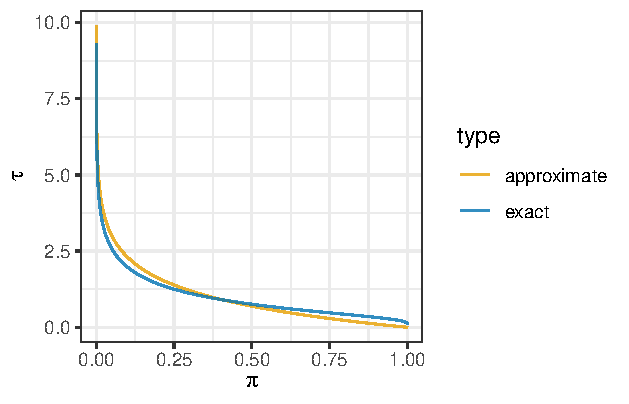
\includegraphics[width=0.6\textwidth]{TL_diffeq.pdf}
  \caption{The scaled number of trophic levels $\tau = T/\lambda_M$ against the baseline extinction probability $\pi$, given by the exact $\tau = -\text{li}(1-\pi)/(1-\pi)$ (Eq.~\ref{eq:BN_lambda_chain_18}) and the approximate $\tau = -\log(\pi)$ (Eq.~\ref{eq:BN_lambda_chain_19}). For practical purposes, the approximate expression is just as good as the exact one.}
  \label{fig:TL_diffeq}
\end{figure}

\begin{figure}[!ht]
  \centering
  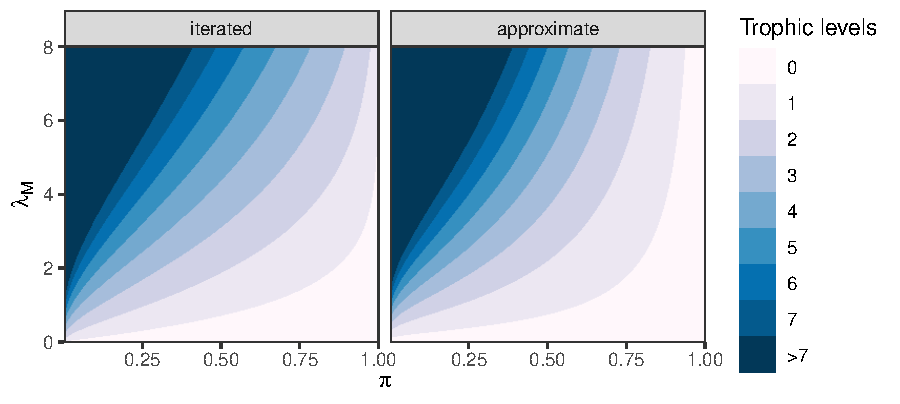
\includegraphics[width=0.93\textwidth]{TL_chain_approx.pdf}
  \caption{The maximum number of trophic levels, as a function of a common baseline extinction probability $\pi$ and the leading eigenvalue of a common landscape matrix $\lambda_M$. Unless $\pi$ is low and $\lambda_M$ high, the metacommunity structure itself puts a cap on the number of possible trophic levels. The left panel is obtained by numerically iterating Eq.~\ref{eq:BN_lambda_chain_5} until $\lambda_i$ drops below the persistence threshold of $1$. The right panel is based on the simple $T = -\lambda_M \log(\pi)$ of Eq.~\ref{eq:BN_lambda_chain_20}. The approximation matches the actual results well.}
  \label{fig:TL_compare}
\end{figure}

Figure~\ref{fig:TL_compare} also reveals that this maximum number is quite limited unless $\pi$ is small and $\lambda_M$ simultaneously large. To get a sense of the typical magnitude of $\lambda_M$, we can use the approximation
\begin{equation}
  \label{eq:lambda_approx}
  \lambda_M \approx G_D \frac{N}{A} \xi^D
\end{equation}
developed by \citet{Grillietal2015}. Here $D$ is the dimensionality of the landscape (in our case $D=2$), $G_D$ is a numerical factor depending on landscape dimensionality and the shape of the dispersal kernel, $N$ is the number of patches, $A$ the total landscape area, and $\xi$ the characteristic dispersal distance. Using data on three real butterfly metapopulations \citep{Hanski1994}, we estimate $\lambda_M$ for each of them in Table~\ref{tab:lambdaM}.

In each case, $\lambda_M$ is in the order of $1$. This means that the ordinate of  Figure~\ref{fig:TL_compare} likely captures an empirically relevant range of possible $\lambda_M$ values. This also implies a potentially quite restricted number of possible trophic levels.

\begin{table}[!ht]
  \centering
  \begin{tabular}{lrrrc}
    species & $N$ & $A$ & $\xi$ & $\lambda_M \approx G_D (N/A) \xi^2$ \\
    \hline
    \textit{Melitaea cinxia} & 50 & 20  & 0.5 & 3.93 \\
    \textit{Hesperia comma}  & 64 & 104 & 0.5 & 0.97 \\
    \textit{Scolitantides orion}  & 70 & 149 & 0.5 & 0.74 \\
  \end{tabular}
  \caption{Estimated leading eigenvalues $\lambda_M$ of the landscape matrices of three butterfly species. Parameters are from \citet[Table~2]{Hanski1994}. Our $\xi$ is defined as the inverse of the original $\alpha$; since $\alpha$ was always set to $2$, here we use $\xi = 0.5$. The $\lambda_M$ are approximated using the formula of \citet{Grillietal2015}. For the exponential kernel and $D=2$, $G_D = 6.283$ (see \citealp[Supplementary Information, Section~5]{Grillietal2015} for the derivation). In each case, $\lambda \sim \mathcal{O}(1)$, suggesting that the ordinate of Figure~\ref{fig:TL_compare} covers an empirically relevant region.}
  \label{tab:lambdaM}
\end{table}

\subsection{One predator with two prey} \label{sec:CtwoR}

Let there be two (not necessarily basal) prey species $R_i$ ($i=1,2$) with marginal extinction probabilities $\delta_i^k$, and one predator $C$ with a baseline of $\pi_C^k$ consuming both. The marginal probability of extinction for the consumer is written
\begin{equation}
  \label{eq:BN_marginal_CRR}
  \begin{split}
    \delta_C^k &= P^k(\neg C|R_1 R_2) P^k(R_1) P^k(R_2) +
    P^k(\neg C|\neg R_1 R_2) P^k(\neg R_1) P^k(R_2)
    \\ &\quad + P^k(\neg C|R_1 \neg R_2) P^k(R_1) P^k(\neg R_2) +
    P^k(\neg C|\neg R_1 \neg R_2) P^k(\neg R_1) P^k(\neg R_2) \ .
  \end{split}
\end{equation}
Using Eqs.~\ref{eq:BN_prob} and \ref{eq:bayesprob}:
\begin{equation}
  \label{eq:BN_marginal_CRR_2}
  \begin{split}
    \delta_C^k &= \pi_C^k(1-\delta_{R_1}^k)(1-\delta_{R_2}^k)p_{R_1}^k p_{R_2}^k
    \\ &\quad + \left[\pi_C^k + (1-\pi_C^k) w(1/2) \right]
    \left[ (1-\delta_{R_1}^k) p_{R_1}^k (1-(1-\delta_{R_2}^k) p_{R_2}^k) +
      (1-\delta_{R_2}^k) p_{R_2}^k (1-(1-\delta_{R_1}^k) p_{R_1}) \right]
    \\ &\quad + (1-(1-\delta_{R_1}^k) p_{R_1}^k) (1-(1-\delta_{R_2}^k)
    p_{R_2}^k) \ .
  \end{split}
\end{equation}
If we further specify $w(1/2)=1/2$, the above expression simplifies to
\begin{equation}
  \label{eq:BN_marginal_CRR_3}
  \delta_C^k = 1 - (1 - \pi_C^k) \left[ \frac{p_{R_1}^k (1 - \delta_{R_1}^k) +
      p_{R_2}^k (1 - \delta_{R_2}^k)}{2} \right] \ ,
\end{equation}
or
\begin{equation}
  \label{eq:BN_marginal_CRR_4}
  \delta_C^k = 1 - (1 - \pi_C^k) \ol{p_R^k (1 - \delta_R^k)} \ ,
\end{equation}
where the overbar denotes the arithmetic average over the prey species $R_i$. In case the prey are basal, $\delta_{R_i}^k = \pi_{R_i}^k$ and the formula is the same as Eq.~\ref{eq:BN_marginal_CR_C_detailed}, with the average replacing the single $p_R^k (1 - \pi_R^k)$ term.

\subsection{One predator with multiple prey} \label{sec:CmanyR}

Let there be $S$ prey species $R_i$ with marginal extinction probabilities $\delta_i^k$, and one consumer $C$ with baseline $\pi_C^k$ eating all prey. We propose the following conjecture: assuming $w(f)=f$ in Eq.~\ref{eq:BN_prob}, the consumer's marginal extinction probability reads
\begin{equation}
  \label{eq:BN_marginal_CmanyR}
  \delta_C^k = 1 - (1 - \pi_C^k) \ol{p_R^k (1 - \delta_R^k)} \ ,
\end{equation}
where the average is taken over all prey species $R_i$. Eq.~\ref{eq:BN_marginal_CmanyR} is a direct generalization of Eq.~\ref{eq:BN_marginal_CRR_4} from two to an arbitrary number of prey items.

We prove this conjecture for the case of identical prey ($\delta_i^k \equiv \delta^k$, $p_{R_i}^k \equiv p_R^k$). Using Eq.~\ref{eq:BN_marginal_example}:
\begin{align}
  \label{eq:BN_marginal_twolayer}
  \delta_C^k &= P^k(\neg C|R_1 R_2 \ldots R_S) \underbrace{P^k(R_1)
               P^k(R_2) \cdots P^k(R_S)}_{[P^k(R)]^S \;
               \text{ [since $P^k(R_i) \equiv P^k(R)$]}}
    \nonumber \\ &+ S P^k(\neg C|\neg R_1 R_2 \ldots R_S)
    \underbrace{P^k(\neg R_1) P^k(R_2) \cdots P^k(R_S)}_{(1-P^k(R)) P^k(R)^{S-1}}
    \\ &+ \binom{S}{2} P^k(\neg C|\neg R_1 \neg R_2 \ldots R_S)
    \underbrace{P^k(\neg R_1) P^k(\neg R_2) \cdots P^k(R_S)}_{(1-P^k(R))^2 P^k(R)^{S-2}}
    \nonumber \\ &+ \cdots
    \nonumber \\ &+ S P^k(\neg C|R_1 \neg R_2 \ldots \neg R_S)
    \underbrace{P^k(R_1) P^k(\neg R_2) \cdots P^k(\neg R_S)}_{(1-P^k(R))^{S-1} P^k(R)}
    \nonumber \\ &+ P^k(\neg C|\neg R_1 \neg R_2 \ldots \neg R_S)
    \underbrace{P^k(\neg R_1) P^k(\neg R_2) \cdots P^k(\neg R_S)}_{(1-P^k(R))^{S}} \ .
                   \nonumber
\end{align}
We used the fact that $P^k(\neg C|\neg R_1 R_2 R_3 \ldots) = P^k(\neg C|R_1 \neg R_2 R_3 \ldots)$ and so on, since the prey are equivalent. Using the notation $P^k(\neg C|k)$ for the probability of $C$ being extinct given that $k$ of its resources are absent, we can rewrite the above as
\begin{equation}
  \label{eq:BN_marginal_twolayer_2}
  \begin{split}
    \delta_C^k &= P^k(\neg C|0) (1-P^k(R))^{0} P^k(R)^{S}
    \\ &+ S P^k(\neg C|1) (b_R^k)^{1} P^k(R)^{S-1}
    \\ &+ \binom{S}{2} P^k(\neg C|2) (1-P^k(R))^{2} P^k(R)^{S-2}
    \\ &+ \cdots
    \\ &+ S P^k(\neg C|S-1) (1-P^k(R))^{S-1} P^k(R)^{1}
    \\ &+ P^k(\neg C|S) (1-P^k(R))^{S} P^k(R)^{0} ,
  \end{split}
\end{equation}
which is compactly written as
\begin{equation}
  \label{eq:BN_marginal_twolayer_3}
  \delta_C^k = \sum_{n=0}^S \binom{S}{n} P^k(\neg C|n) (1-P^k(R))^n P^k(R)^{S-n} .
\end{equation}
Since we use the linear response function $w(f) = f$, and $f = n/S$ is the fraction of resources absent, $P^k(\neg C|n)$ can be written as $\pi_C^k + (1-\pi_C^k) (n / S)$ (Eq.~\ref{eq:BN_prob}):
\begin{equation}
  \label{eq:BN_marginal_twolayer_4}
  \begin{split}
    \delta_C^k = P^k(\neg C) &= \sum_{n=0}^S \binom{S}{n} \left[ \pi_C^k +
      (1-\pi_C^k) \frac{n}{S} \right] (1-P^k(R))^n P^k(R)^{S-n}
    \\ &= \pi_C^k \underbrace{\sum_{n=0}^S \binom{S}{n} (1-P^k(R))^n
      P^k(R)^{S-n}}_{1} + \frac{1-\pi_C^k}{S} \underbrace{\sum_{n=0}^S
      n \binom{S}{n} (1-P^k(R))^n P^k(R)^{S-n}}_{S (1-P^k(R))} .
  \end{split}
\end{equation}
The first sum is over the binomial distribution and therefore equal to 1; the second sum is over $n$ times the binomial distribution and is therefore equal to its mean, $S \pi_R^k$. We therefore end up with $\delta_C^k = \pi_C^k + (1 - \pi_C^k) (1 - P^k(R))$. Substituting $P^k(R) = p_{R}^k (1 - \delta_R^k)$ (Eq.~\ref{eq:bayesprob}) and rearranging, we recover Eq.~\ref{eq:BN_marginal_CmanyR}.

Though a strict proof is missing, the formula held true even for non-equivalent prey species, without exception. We therefore proceed by assuming that Eq.~\ref{eq:BN_marginal_CmanyR} holds for this general case as well, even though we emphasize that this is not yet strictly proven.

\subsection{Two strict trophic levels} \label{sec:2level}

Consider $S$ basal prey species $R_1,\ldots, R_S$, and $L$ consumers $C_1,\ldots,C_S$. For the prey, $\delta_{R_i}^k = \pi_{R_i}^k$. Let $\mathcal{P}(A,B,\ldots)$ denote the set of prey jointly consumed by species $A$, $B$, \ldots. To determine the marginal extinction probabilities of the consumers, we can apply the argument of Section~\ref{sec:CmanyR} to each consumer species individually:
\begin{equation}
  \label{eq:BN_marginal_twolevel_C}
  \delta_{C_i}^k = 1 - (1 - \pi_{C_i}^k) \ol{p_{\mathcal{P}(C_i)}^k
    (1 - \delta_{\mathcal{P}(C_i)}^k)} \ ,
\end{equation}
where the arithmetic average is taken over the set of $C_i$'s prey, $\mathcal{P}(C_i)$.

\subsection{Multispecies trophic chain} \label{sec:mtc}

In this case we have several trophic levels, each with a certain number of species, and species at a given level can only consume species from one level below. Eq.~\ref{eq:BN_marginal_twolevel_C} holds for any two trophic levels, so it can be used recursively to find the marginal extinction probabilities of any species, starting from the basal level where for each basal species $i$, we have $\delta_i^k = \pi_i^k$. For another species $i$ on the second level, applying Eq.~\ref{eq:BN_marginal_twolevel_C} yields
\begin{equation}
  \label{eq:BN_mtc}
  \delta_i^k = 1 - (1 - \pi_i^k) \ol{p_{\mathcal{P}(i)}^k
    (1 - \pi_{\mathcal{P}(i)}^k)} \ ,
\end{equation}
and for the third,
\begin{equation}
  \label{eq:BN_mtc_2}
  \delta_i^k = 1 - (1 - \pi_i^k) \ol{p_{\mathcal{P}(i)}^k
    (1-\pi_{\mathcal{P}(i)}^k)\ol{p_{\mathcal{P}(\mathcal{P}(i))}^k
      (1-\pi_{\mathcal{P}(\mathcal{P}(i))}^k)}} \ .
\end{equation}
Here the the higher overbar averages over the prey (on level $2$) of the focal species $i$, while the lower overbar averages over the prey (on level $1$) of those consumers (on level $2$) that are eaten by $i$. The notation $\mathcal{P}(\mathcal{P}(i))$ reads ``the prey items of the set of species which are prey items of species $i$''.

\subsection{Simple omnivory module}

Let there be a single basal resource $R$, a consumer $C$ eating the resource, and a top species $T$ eating both the consumer and the resource. We assume $w(f)=f$.

\textit{\textbf{Step 1: Solve for the extinction probabilities using the Bayesian network approach.}}
The basal and consumer species are the same as they were in Section~\ref{sec:CR}, so their probabilities are given by Eqs.~\ref{eq:BN_marginal_CR_R_detailed} and \ref{eq:BN_marginal_CR_C_detailed}. For the top species, we write
\begin{equation}
  \label{eq:BN_marginal_omniv}
  \begin{split}
    \delta_T^k &= P^k(\neg T|R C) P^k(R) P^k(C) + P^k(\neg T|\neg R C)
    P^k(\neg R) P^k(C) \\ &\quad + P^k(\neg T|R \neg C) P^k(R) P^k(\neg C) +
    P^k(\neg T|\neg R \neg C) P^k(\neg R) P^k(\neg C) \ .
  \end{split}
\end{equation}
Using Eq.~\ref{eq:BN_prob} with $w(f)=f$:
\begin{equation}
  \label{eq:BN_marginal_omniv_2}
  \begin{split}
    \delta_T^k &= \pi_T^k P^k(R) P^k(C) + \left( \frac{1 + \pi_T^k}{2} \right)
    \left[ P^k(R) (1-P^k(C) + P^k(C) (1-P^k(R))) \right] + (1-P^k(C)) (1-P^k(R))
    \\ &= 1 - \frac{1}{2} (1 - \pi_T^k) \left[ P^k(R) + P^k(C) \right] \ .
  \end{split}
\end{equation}
Applying Eq.~\ref{eq:bayesprob} and Eqs.~\ref{eq:BN_marginal_CR_R_detailed}-\ref{eq:BN_marginal_CR_C_detailed} for the resource and consumer:
\begin{equation}
  \label{eq:BN_marginal_omniv_3}
  \delta_T^k = 1 - \frac{1}{2} (1 - \pi_T^k) \left[ (1-\pi_R^k) p_R^k +
    (1-\pi_C^k) (1-\pi_R^k) p_C^k p_R^k \right] \ ,
\end{equation}
or, after simplifying,
\begin{equation}
  \label{eq:BN_marginal_omniv_4}
  \delta_T^k = 1 - (1 - \pi_T^k) \left( \frac{1 + p_C^k (1-\pi_C^k)}{2} \right)
  (1-\pi_R^k) p_R^k \ .
\end{equation}
Writing out the probabilities for all three species:
\begin{align}
  \label{eq:BN_marginal_omniv_R}
  \delta_R^k &= \pi_R^k \ , \\
  \label{eq:BN_marginal_omniv_C}
  \delta_C^k & = 1 - (1-\pi_C^k) (1-\pi_R^k) p_R^k \ , \\
  \label{eq:BN_marginal_omniv_T}
  \delta_T^k &= 1 - (1 - \pi_T^k) \left( \frac{1 + p_C^k (1-\pi_C^k)}{2} \right)
               (1-\pi_R^k) p_R^k \ .
\end{align}
Comparing these results with Eqs.~\ref{eq:BN_marginal_chain_R}-\ref{eq:BN_marginal_chain_T}, we see that the only difference is in $\delta_T^k$: in the omnivory scenario, $(1 - \pi_C^k) p_C^k$ is replaced by $(1 + (1 - \pi_C^k) p_C^k) / 2$. Since $(1 - \pi_C^k) p_C^k$ is the product of two probabilities, it is between $0$ and $1$. But then, $(1 + (1 - \pi_C^k) p_C^k) / 2 > (1 - \pi_C^k) p_C^k$ holds, and so $\delta_T^k$ in the omnivory case is always lower than $\delta_T^k$ in the corresponding food chain scenario---a result in line with common sense.

\textit{\textbf{Step 2: Obtain the metapopulation capacity of each species.}}
The Jacobian matrices of the principal maps evaluated at zero, from Eq.~\ref{eq:pmjac}, read
\begin{align}
  \label{eq:BN_A_omniv_R}
  A_R^{kl} &= -\frac{M_R^{kl}}{\log(1 - \pi_R^k)} \ , \\
  \label{eq:BN_A_omniv_C}
  A_C^{kl} &= -\frac{M_C^{kl}}{\log[(1 - \pi_C^k) (1 - \pi_R^k) p_R^k]} \ , \\
  \label{eq:BN_A_omniv_T}
  A_T^{kl} &= -\frac{M_T^{kl}}{\log \left[ (1 - \pi_T^k) \left( 1 + p_C^k
             (1-\pi_C^k) \right) (1-\pi_R^k) p_R^k / 2 \right] } \ .
\end{align}
The metapopulation capacities are the leading eigenvalues of the three matrices above.

\textit{\textbf{Step 3: Approximate metapopulation capacities analytically.}}
Using the nonspatial baseline extinction probabilities and average patch occupancies (\textit{Step 3a}):
\begin{align}
  \label{eq:BN_A_omniv_R_nonspatial}
  A_R^{kl} &\approx -\frac{M_R^{kl}}{\log(1 - \pi_R)} \ , \\
  \label{eq:BN_A_omniv_C_nonspatial}
  A_C^{kl} &\approx -\frac{M_C^{kl}}{\log[(1 - \pi_C) (1-\pi_R)\ol{p}_R]} \ , \\
  \label{eq:BN_A_omniv_T_nonspatial}
  A_T^{kl} &\approx -\frac{M_T^{kl}}{\log \left[ (1 - \pi_T) \left( 1 + \ol{p}_C
             (1-\pi_C) \right) (1-\pi_R) \ol{p}_R / 2 \right] } \ ,
\end{align}
with leading eigenvalues
\begin{align}
  \label{eq:BN_lambda_omniv_R_nonspatial}
  \lambda_R &\approx -\frac{\lambda_{M_R}}{\log(1 - \pi_R)} \ , \\
  \label{eq:BN_lambda_omniv_C_nonspatial}
  \lambda_C &\approx -\frac{\lambda_{M_C}}{\log[(1 - \pi_C)
              (1-\pi_R)\ol{p}_R]} \ , \\
  \label{eq:BN_lambda_omniv_T_nonspatial}
  \lambda_T &\approx -\frac{\lambda_{M_T}}{\log \left[ (1 - \pi_T) \left( 1 +
              \ol{p}_C (1-\pi_C) \right) (1-\pi_R) \ol{p}_R / 2 \right] } \ , \\
\end{align}
where $\lambda_{M_i}$ is the leading eigenvalue of the $i$th landscape matrix $M_i^{kl}$. Using Eq.~\ref{eq:papprox} (\textit{Step 3b}):
\begin{align}
  \label{eq:BN_lambda_omniv_R_nonspatial_2}
  \lambda_R &\approx -\frac{\lambda_{M_R}}{\log(1 - \pi_R)} \ , \\
  \label{eq:BN_lambda_omniv_C_nonspatial_2}
  \lambda_C &\approx -\frac{\lambda_{M_C}}{\log\left[ (1 - \pi_C) (1 - \pi_R)
              \left( 1+\dfrac{\log(1-\pi_R)}{\lambda_{M_R}}\right)\right]} \ , \\
  \label{eq:BN_lambda_omniv_T_nonspatial_2}
  \lambda_T &\approx -\frac{\lambda_{M_T}}{\log \left[ \frac{(1-\pi_R) (1-\pi_T)
              \left[ \lambda_{M_R} + \log(1-\pi_R) \right] \left[
              (2-\pi _C) \lambda_{M_C} + (1-\pi_C) \log \left[ \frac{1-\pi_C
              (1-\pi_R) \left( \lambda_{M_R} + \log \left(1 - \pi_R \right)
              \right)}{\lambda_{M_R}} \right] \right]}{2 \lambda_{M_C}
              \lambda_{M_R}} \right]} \ .
\end{align}


\section{Food webs under habitat loss}

\subsection{Generating model food webs} \label{sec:allo}

We generated food webs (adjacency matrices of who eats whom) based on the allometric framework of \citet{Schneider2016}. This topological network model is an extension of the niche model \citep{Williams2000} and accounts for allometric degree distributions and known scaling relationships between species' body mass and trophic level \citep{Riede2011Size-basedExtinctions}. Each species $i$ is characterized by its average adult body mass $m_i$. We uniformly sample $\logten$ body masses of $S_C$ consumer species from the interval $[2, 12]$, and of $S_B$ basal species from $[0, 6]$. Given these body masses, the probability $L_{ij}$ that consumer $i$ has a feeding link to species $j$ is given by
\begin{equation}
  \label{eq:feeding_prob}
  L_{ij} = \left[ \frac{1}{R_{\text{opt}}} \frac{m_i}{m_j} \exp
    \left( 1 - \frac{1}{R_{\text{opt}}} \frac{m_i}{m_j} \right) \right]^{\gamma}
\end{equation}
\citep{Schneider2016}, where $R_{\text{opt}} = 100$ is the body mass ratio between consumers and their prey that yields the maximum probability of predation (the ``optimal'' ratio, from the point of view of the consumer), and $\gamma = 2$ is the width of the function (the range of body masses likely eaten by consumers). Of all the webs generated by this method, we only kept those that were acyclic, as this is required by the Bayesian network approach.

\subsection{Trophic levels} \label{sec:tls}

The prey-averaged trophic level $T_i$ of species $i$ is defined as
\begin{equation}
  \label{eq:patl1}
  T_i = 1 + \sum_{j=1}^S T_j B_{ji}
\end{equation}
\citep{WilliamsMartinez2004}. Here $B_{ij}$ is the $(i,j)$the entry of the food web's adjacency matrix, divided by the number of prey items of species $i$. In matrix notation, $\mathbf{T} = \mathbf{e} + \mathbf{T} \mathbf{B}^{\mathrm{T}}$, where $\mathbf{e}$ is the vector of all $1$'s, and $\mathbf{B}^{\mathrm{T}}$ is the transpose of $\mathbf{B}$. We solve for the vector of trophic levels $\mathbf{T}$:
\begin{equation}
  \label{eq:patl2}
  \mathbf{T} = \left( \mathbf{I} - \mathbf{B}^{\mathrm{T}} \right)^{-1}
  \mathbf{e} \ ,
\end{equation}
$\mathbf{I}$ being the identity matrix. For the purposes of creating figures, we then grouped species based on the nearest half-integer value to their trophic level $T_i$.


\section{Supplementary model results} \label{sec:suppsim}

\subsection{Removing patches based on the patch value rankings of basal species}

Patch removal proceeds as described in the main text.

\begin{figure}[!hp]
  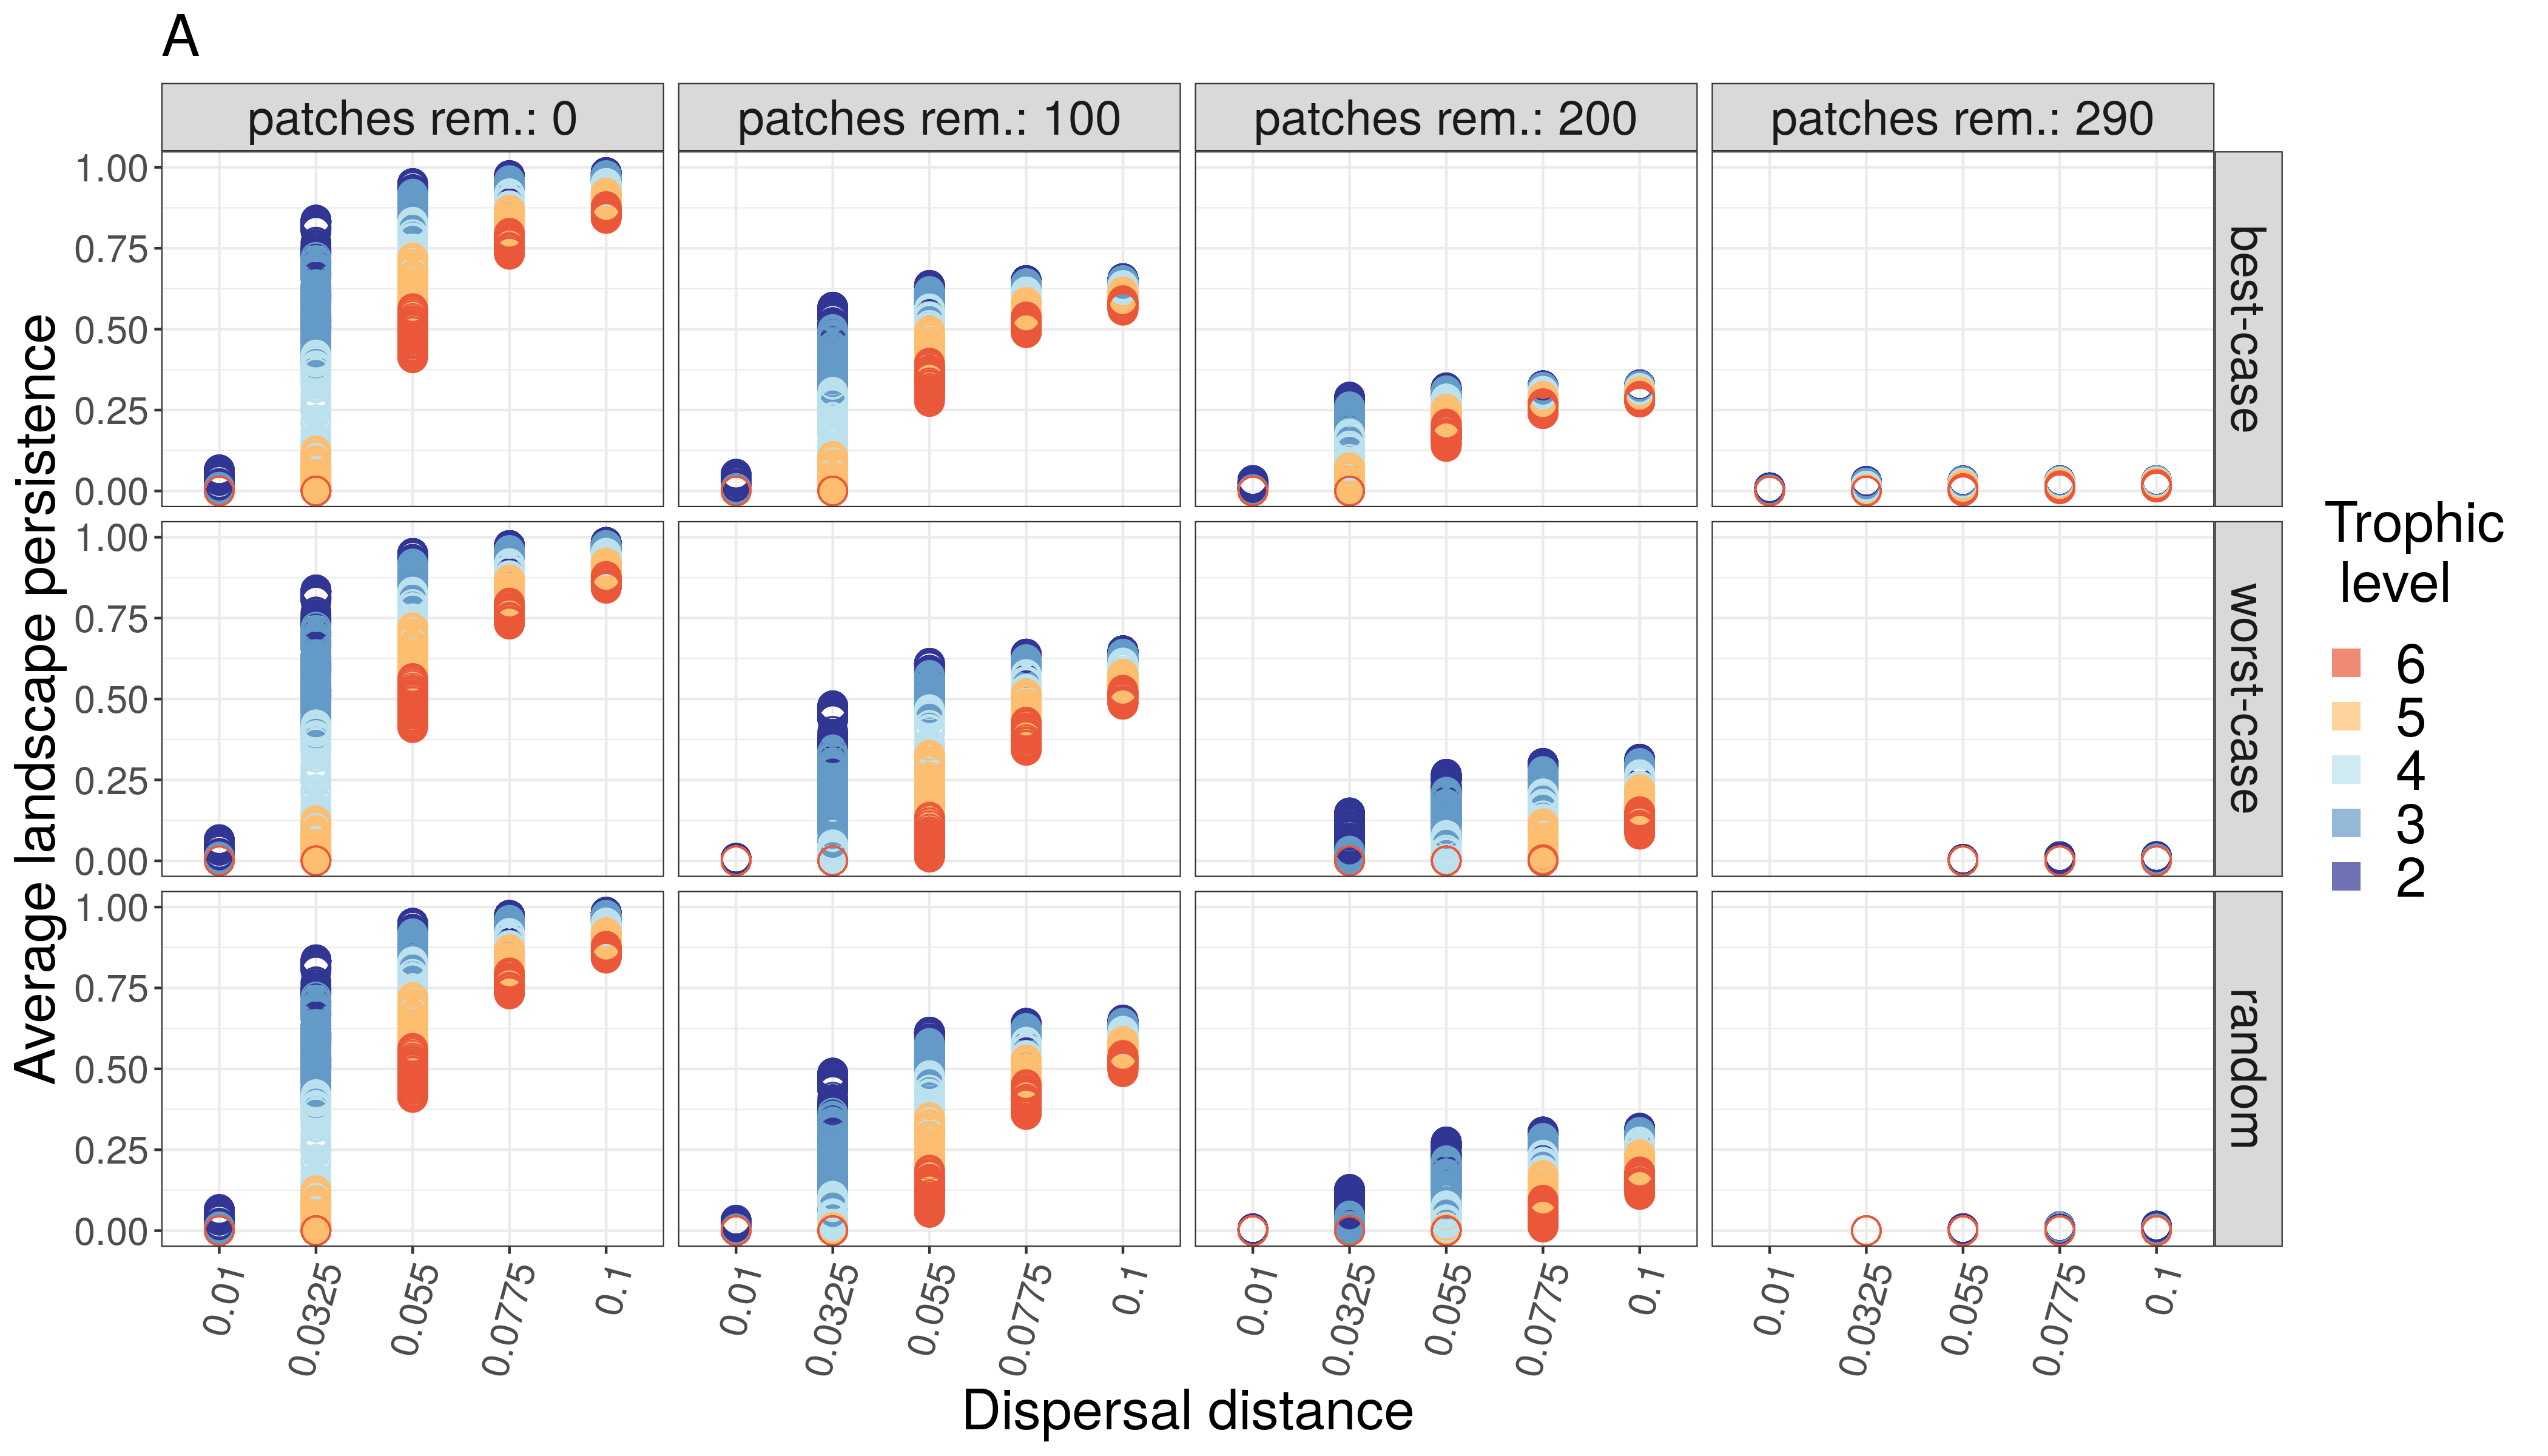
\includegraphics[width=0.8\textwidth,valign=t]{sump_Model_food_web_with_300_consumer_and_100_basal_species_basal_1_1.png}
  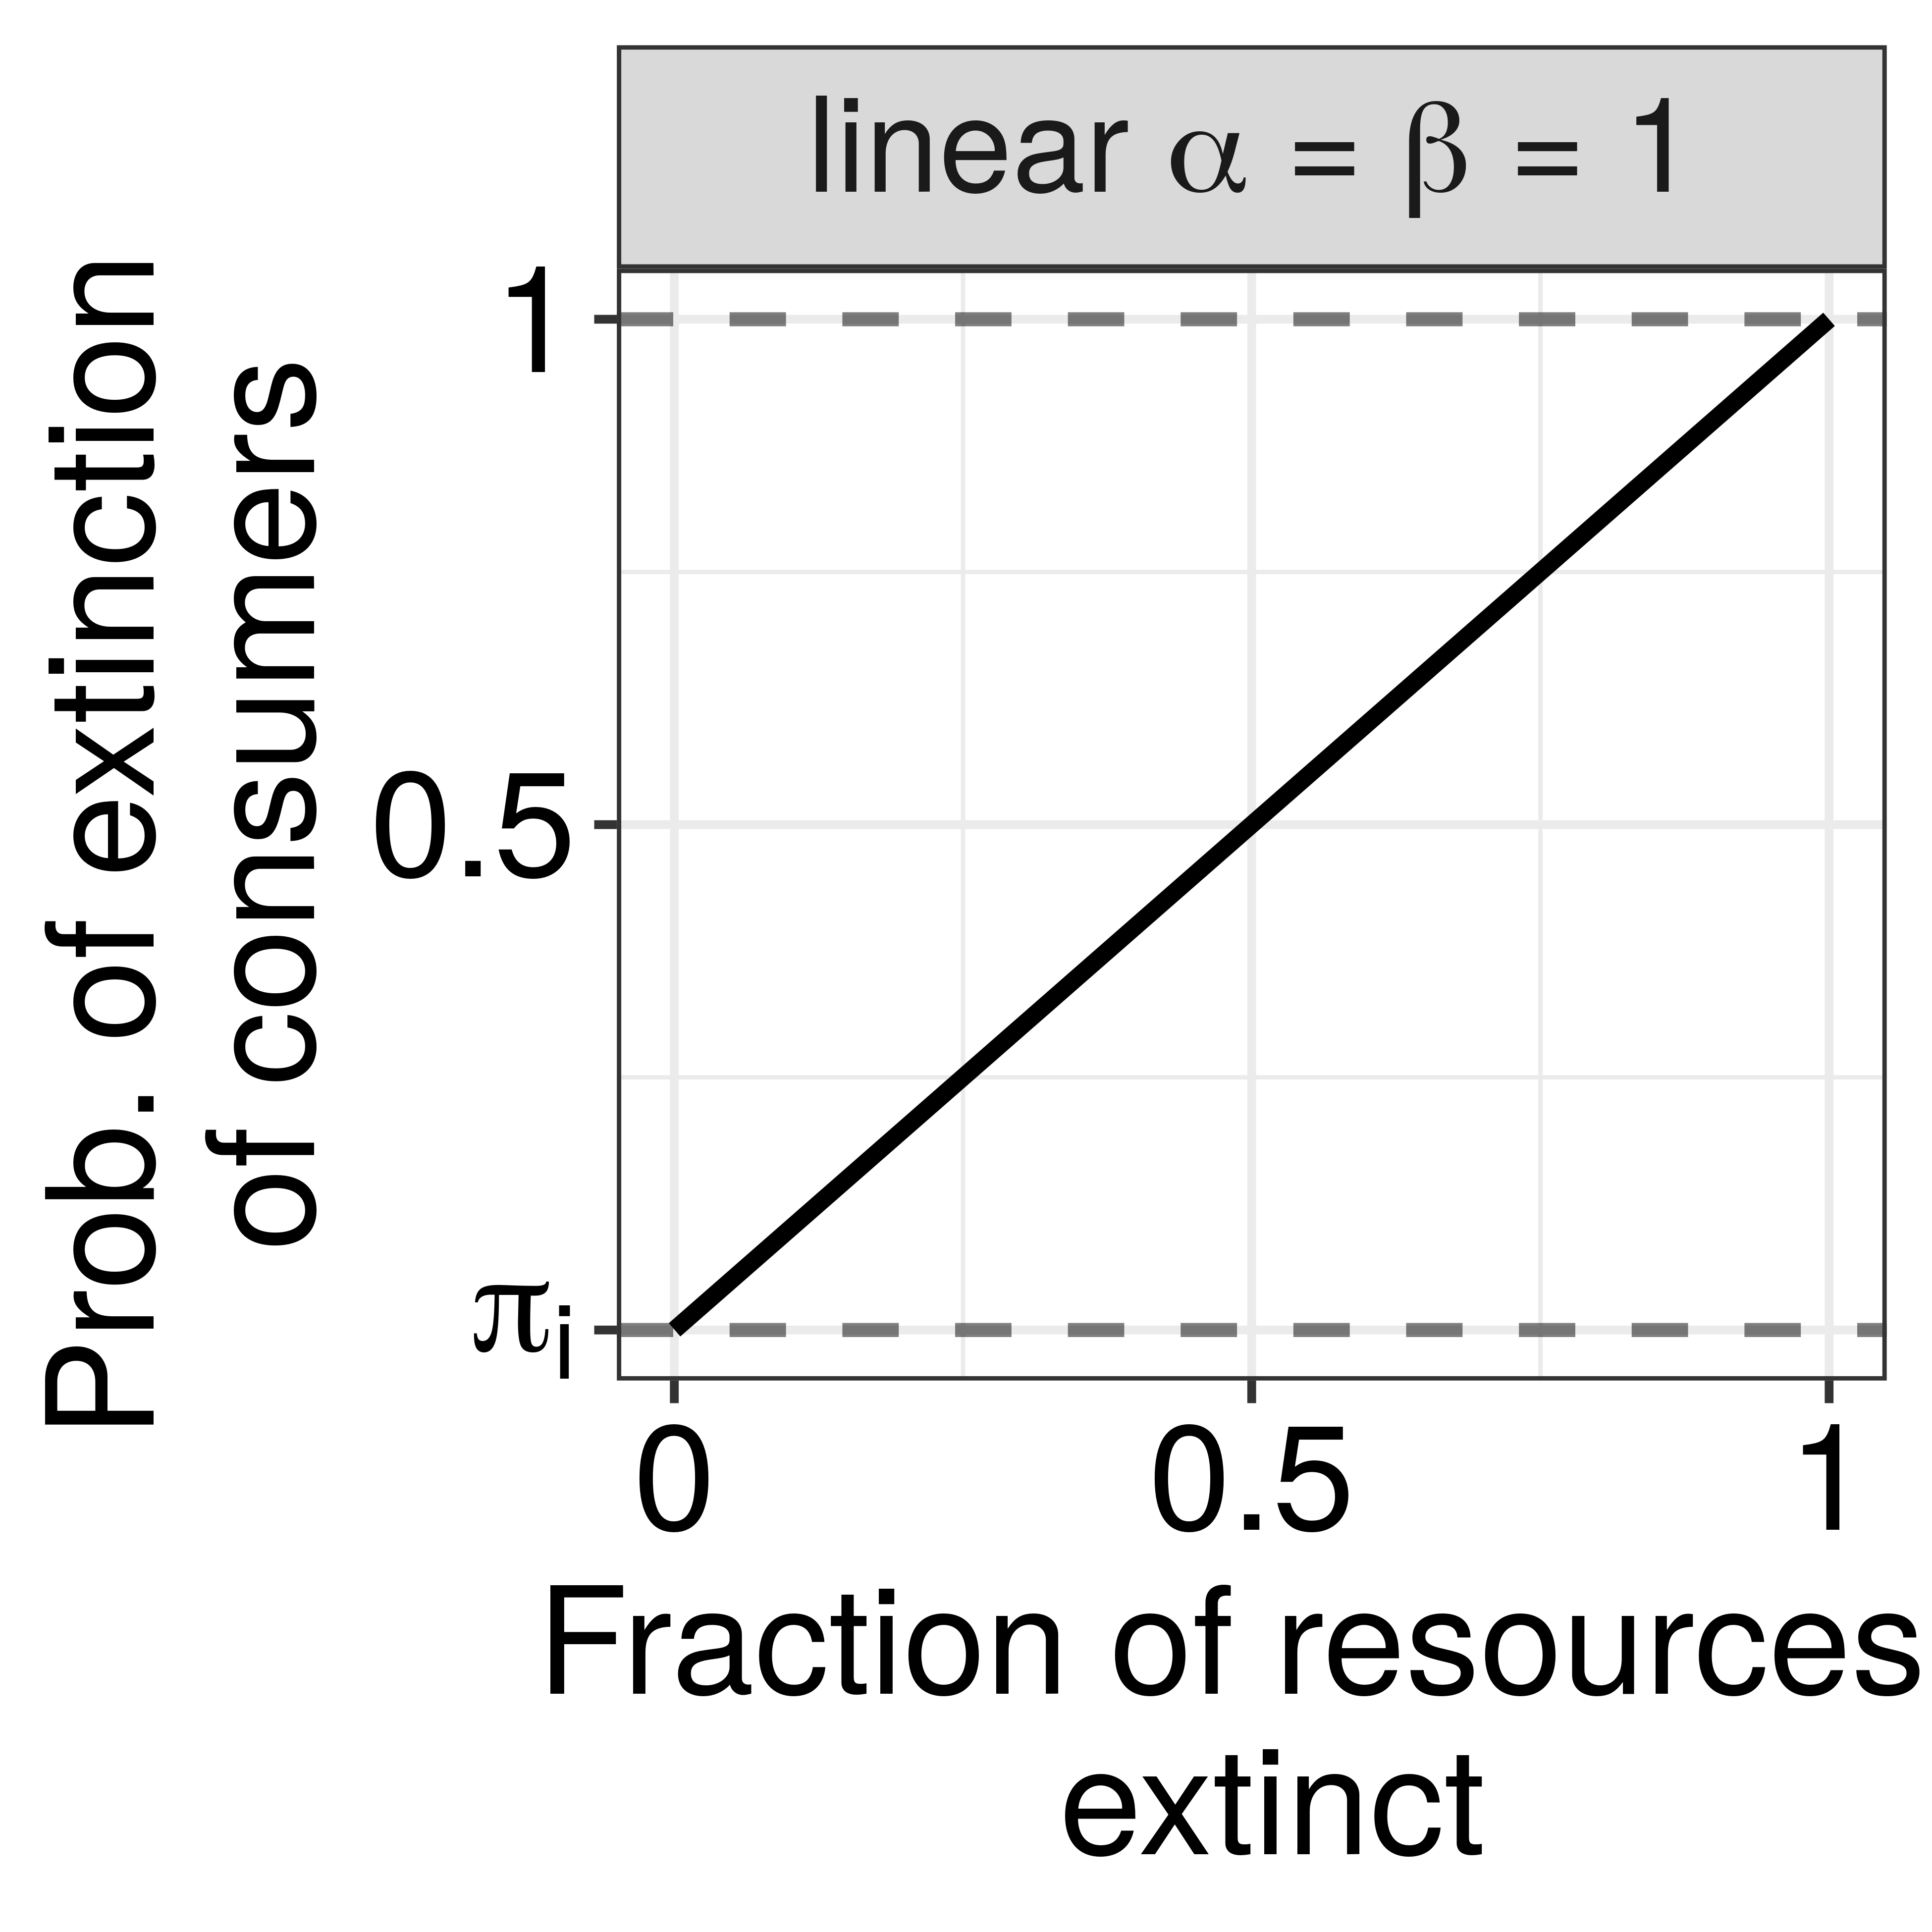
\includegraphics[width=0.19\textwidth,valign=t]{fform_1_1.png}
  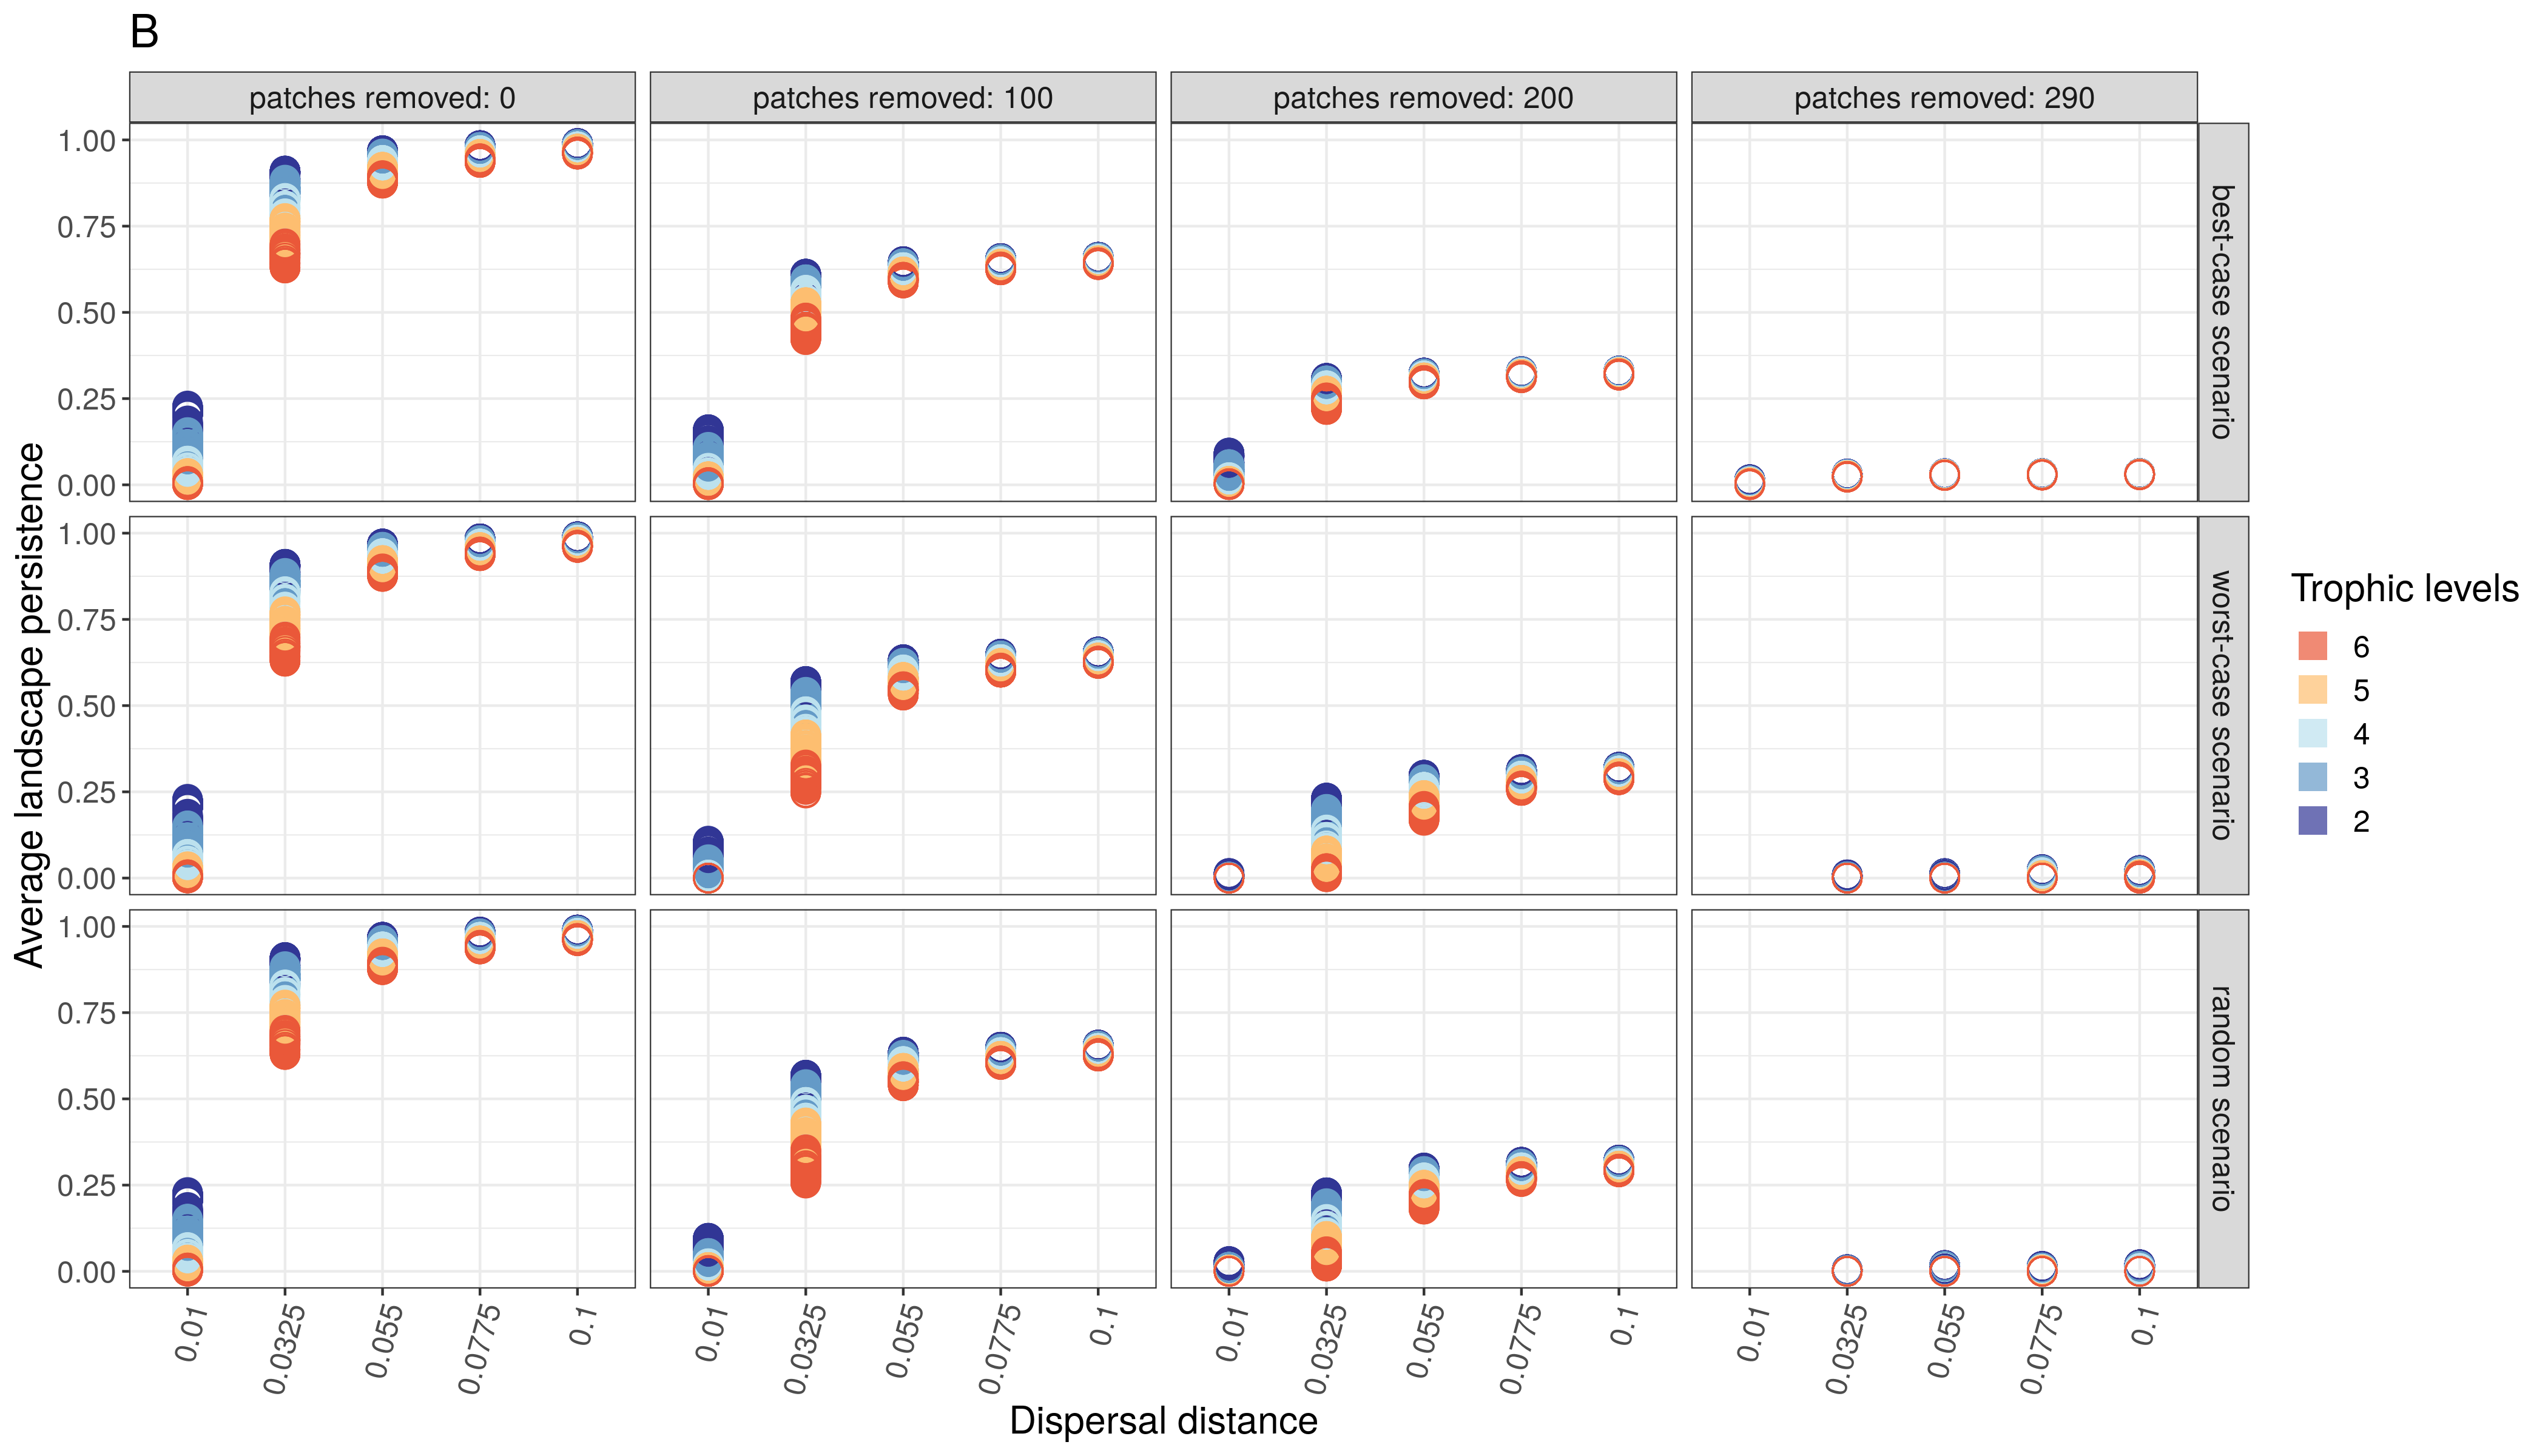
\includegraphics[width=0.8\textwidth,valign=t]{sump_Model_food_web_with_300_consumer_and_100_basal_species_basal_5_1.png}
    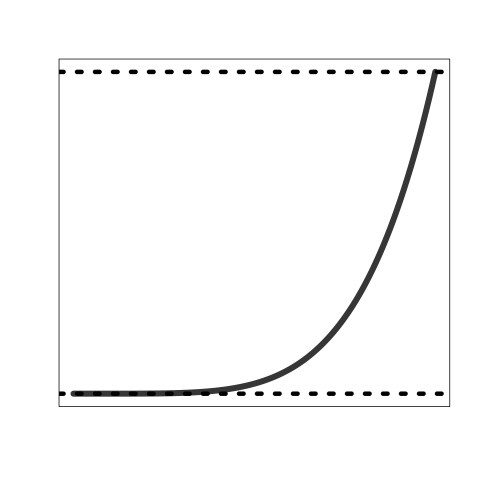
\includegraphics[width=0.19\textwidth,valign=t]{fform_5_1.png}
 \caption{Average species persistence against dispersal distance, in a model food web with 300 consumer and 100 basal species. Average persistence of species $i$ is measured by $\sum_{k=1}^N p_i^k/N$, with the understanding that $N$ is the number of patches over the unperturbed landscape and $p_i^k = 0$ on removed patches. A-D are for different functional forms of a consumer's response to the loss of resources (top right insets). Species are grouped into trophic levels (color legends). Rows indicate patch-removal scenario (best-case, worst-case, and random); columns the number of patches removed from the full landscape. Baseline extinction probabilities $\pi_i$ increase with trophic level (trophic level-based, TLB) and dispersal distances $\xi_i$ range between between $0.01$ and $0.1$, having the same value across all species in any one parameterization.}
 \label{S_fig:patchloss_300_100_distance_1}
\end{figure}

\begin{figure}\ContinuedFloat
  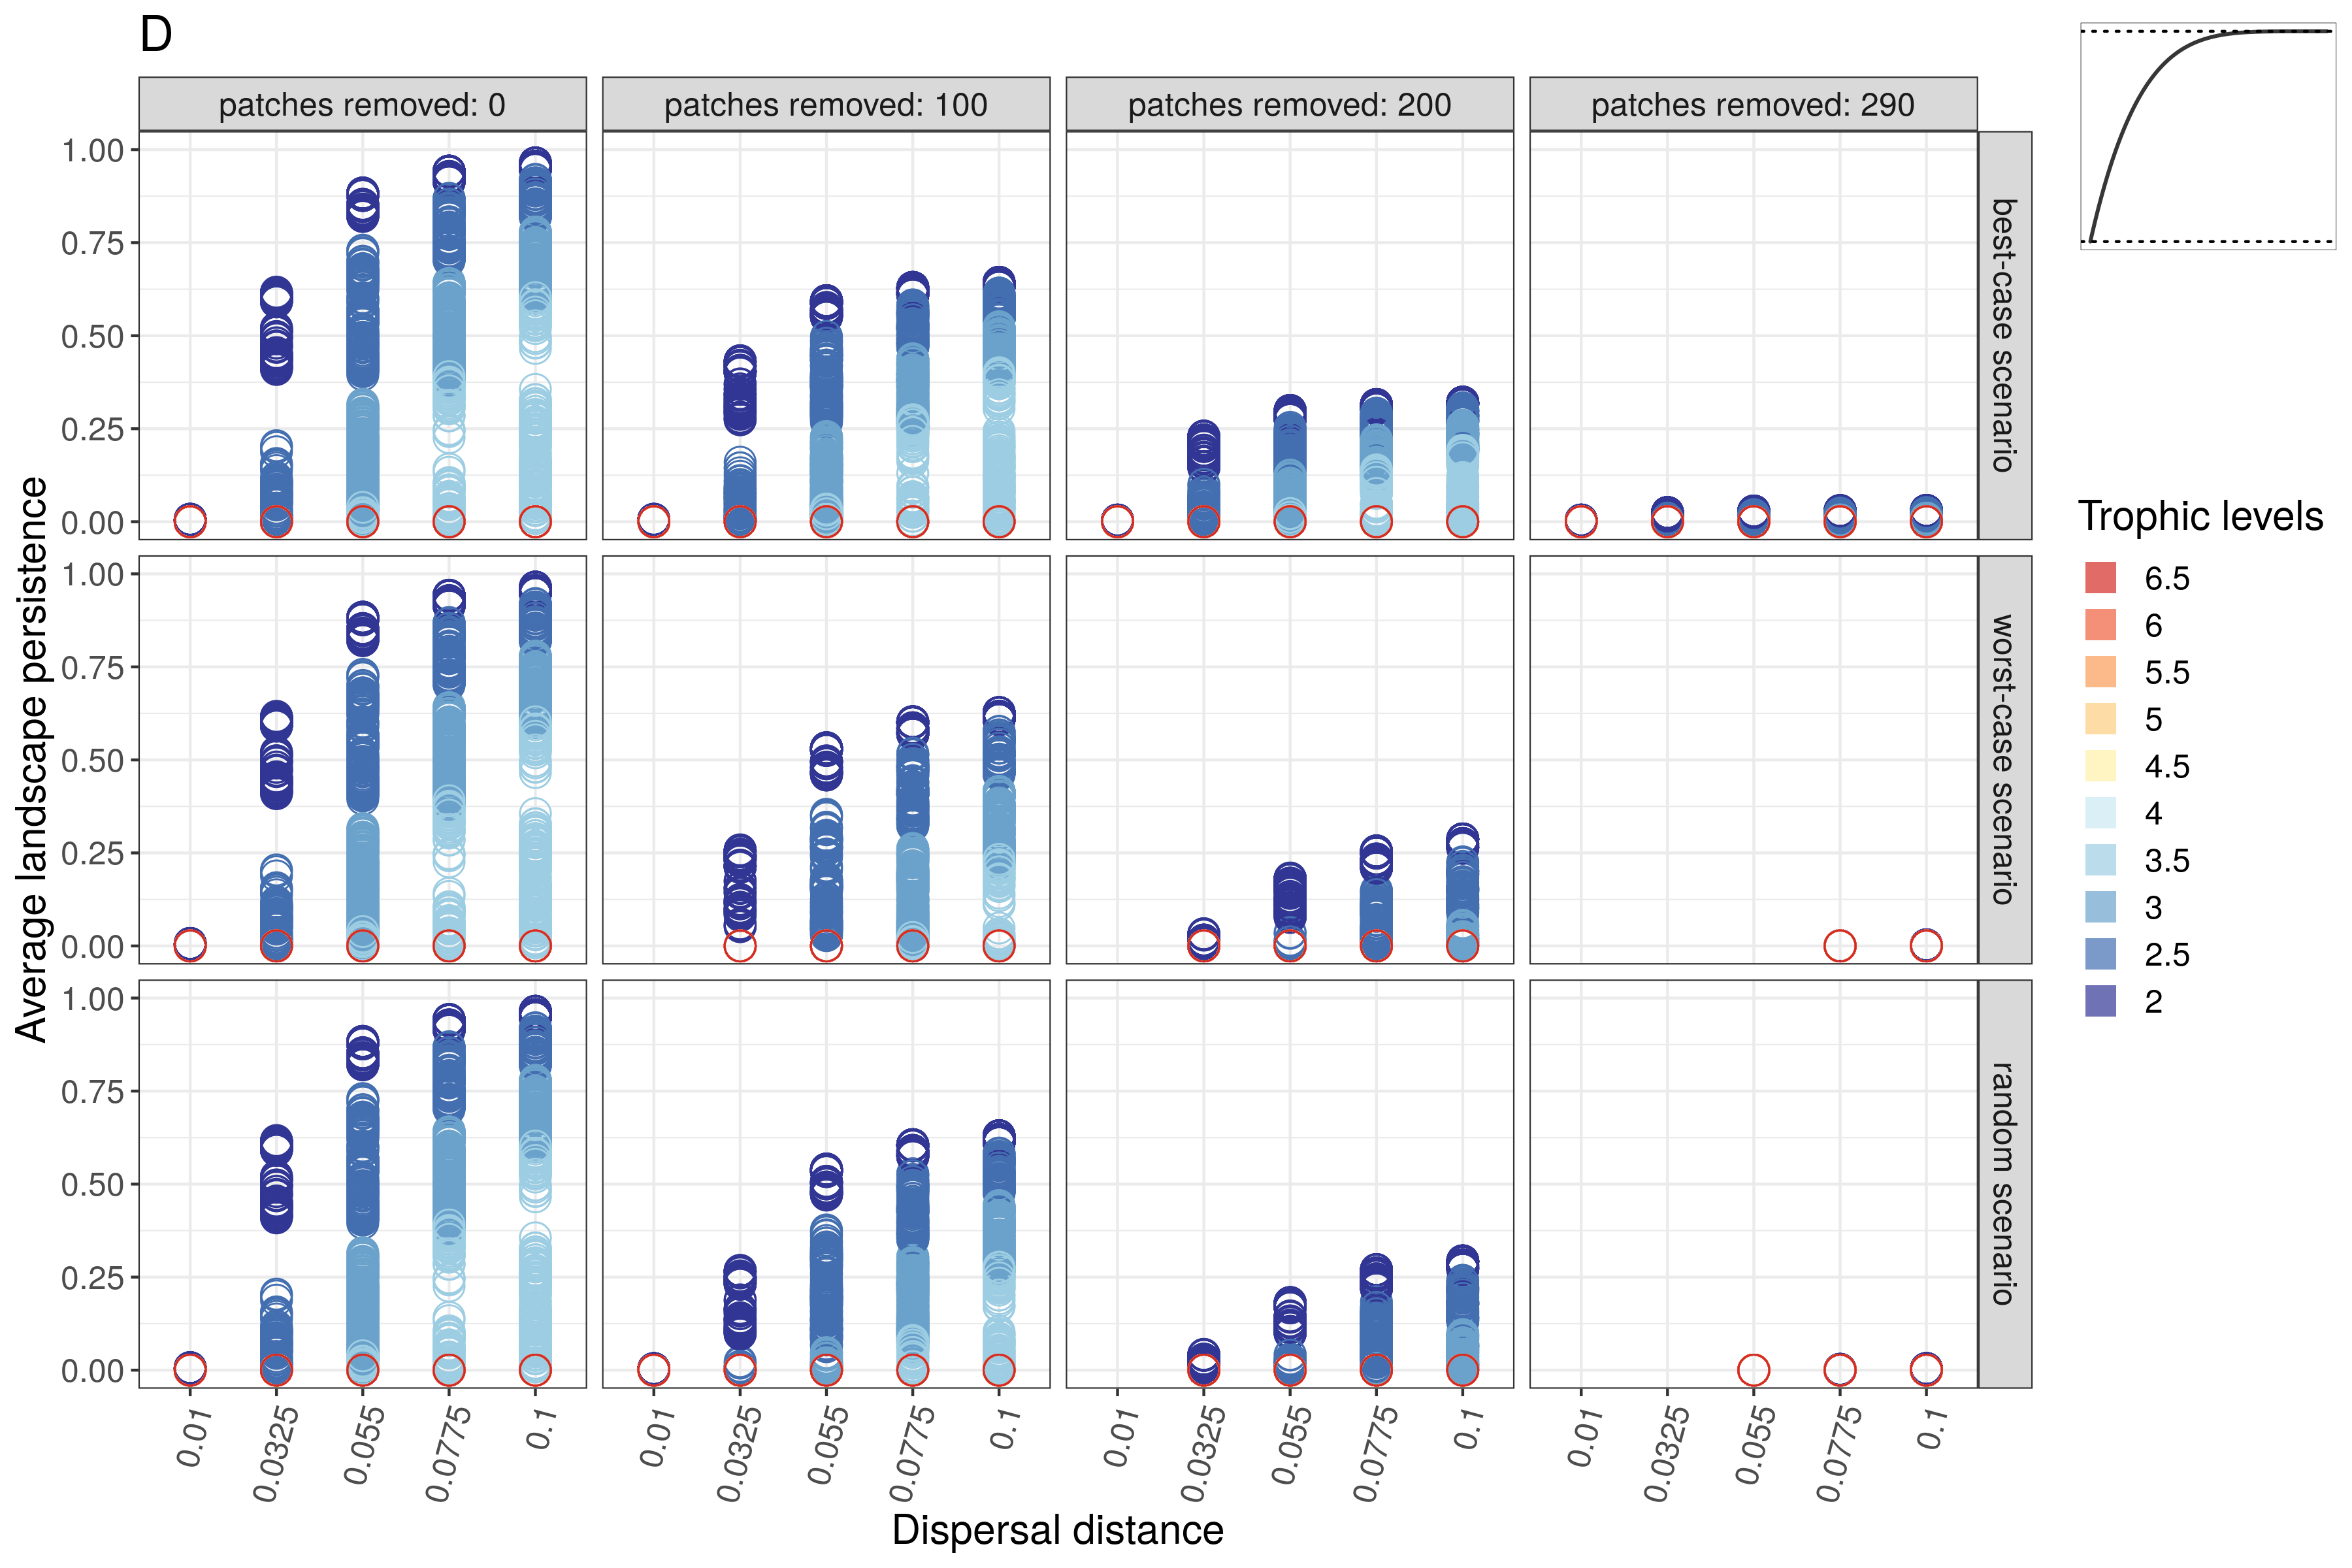
\includegraphics[width=0.8\textwidth,valign=t]{sump_Model_food_web_with_300_consumer_and_100_basal_species_basal_1_5.png}
  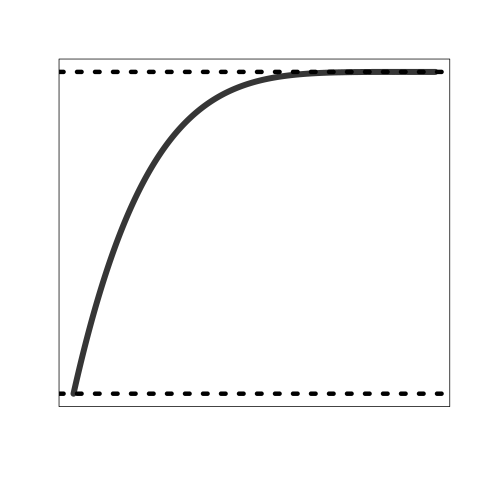
\includegraphics[width=0.19\textwidth,valign=t]{fform_1_5.png}
  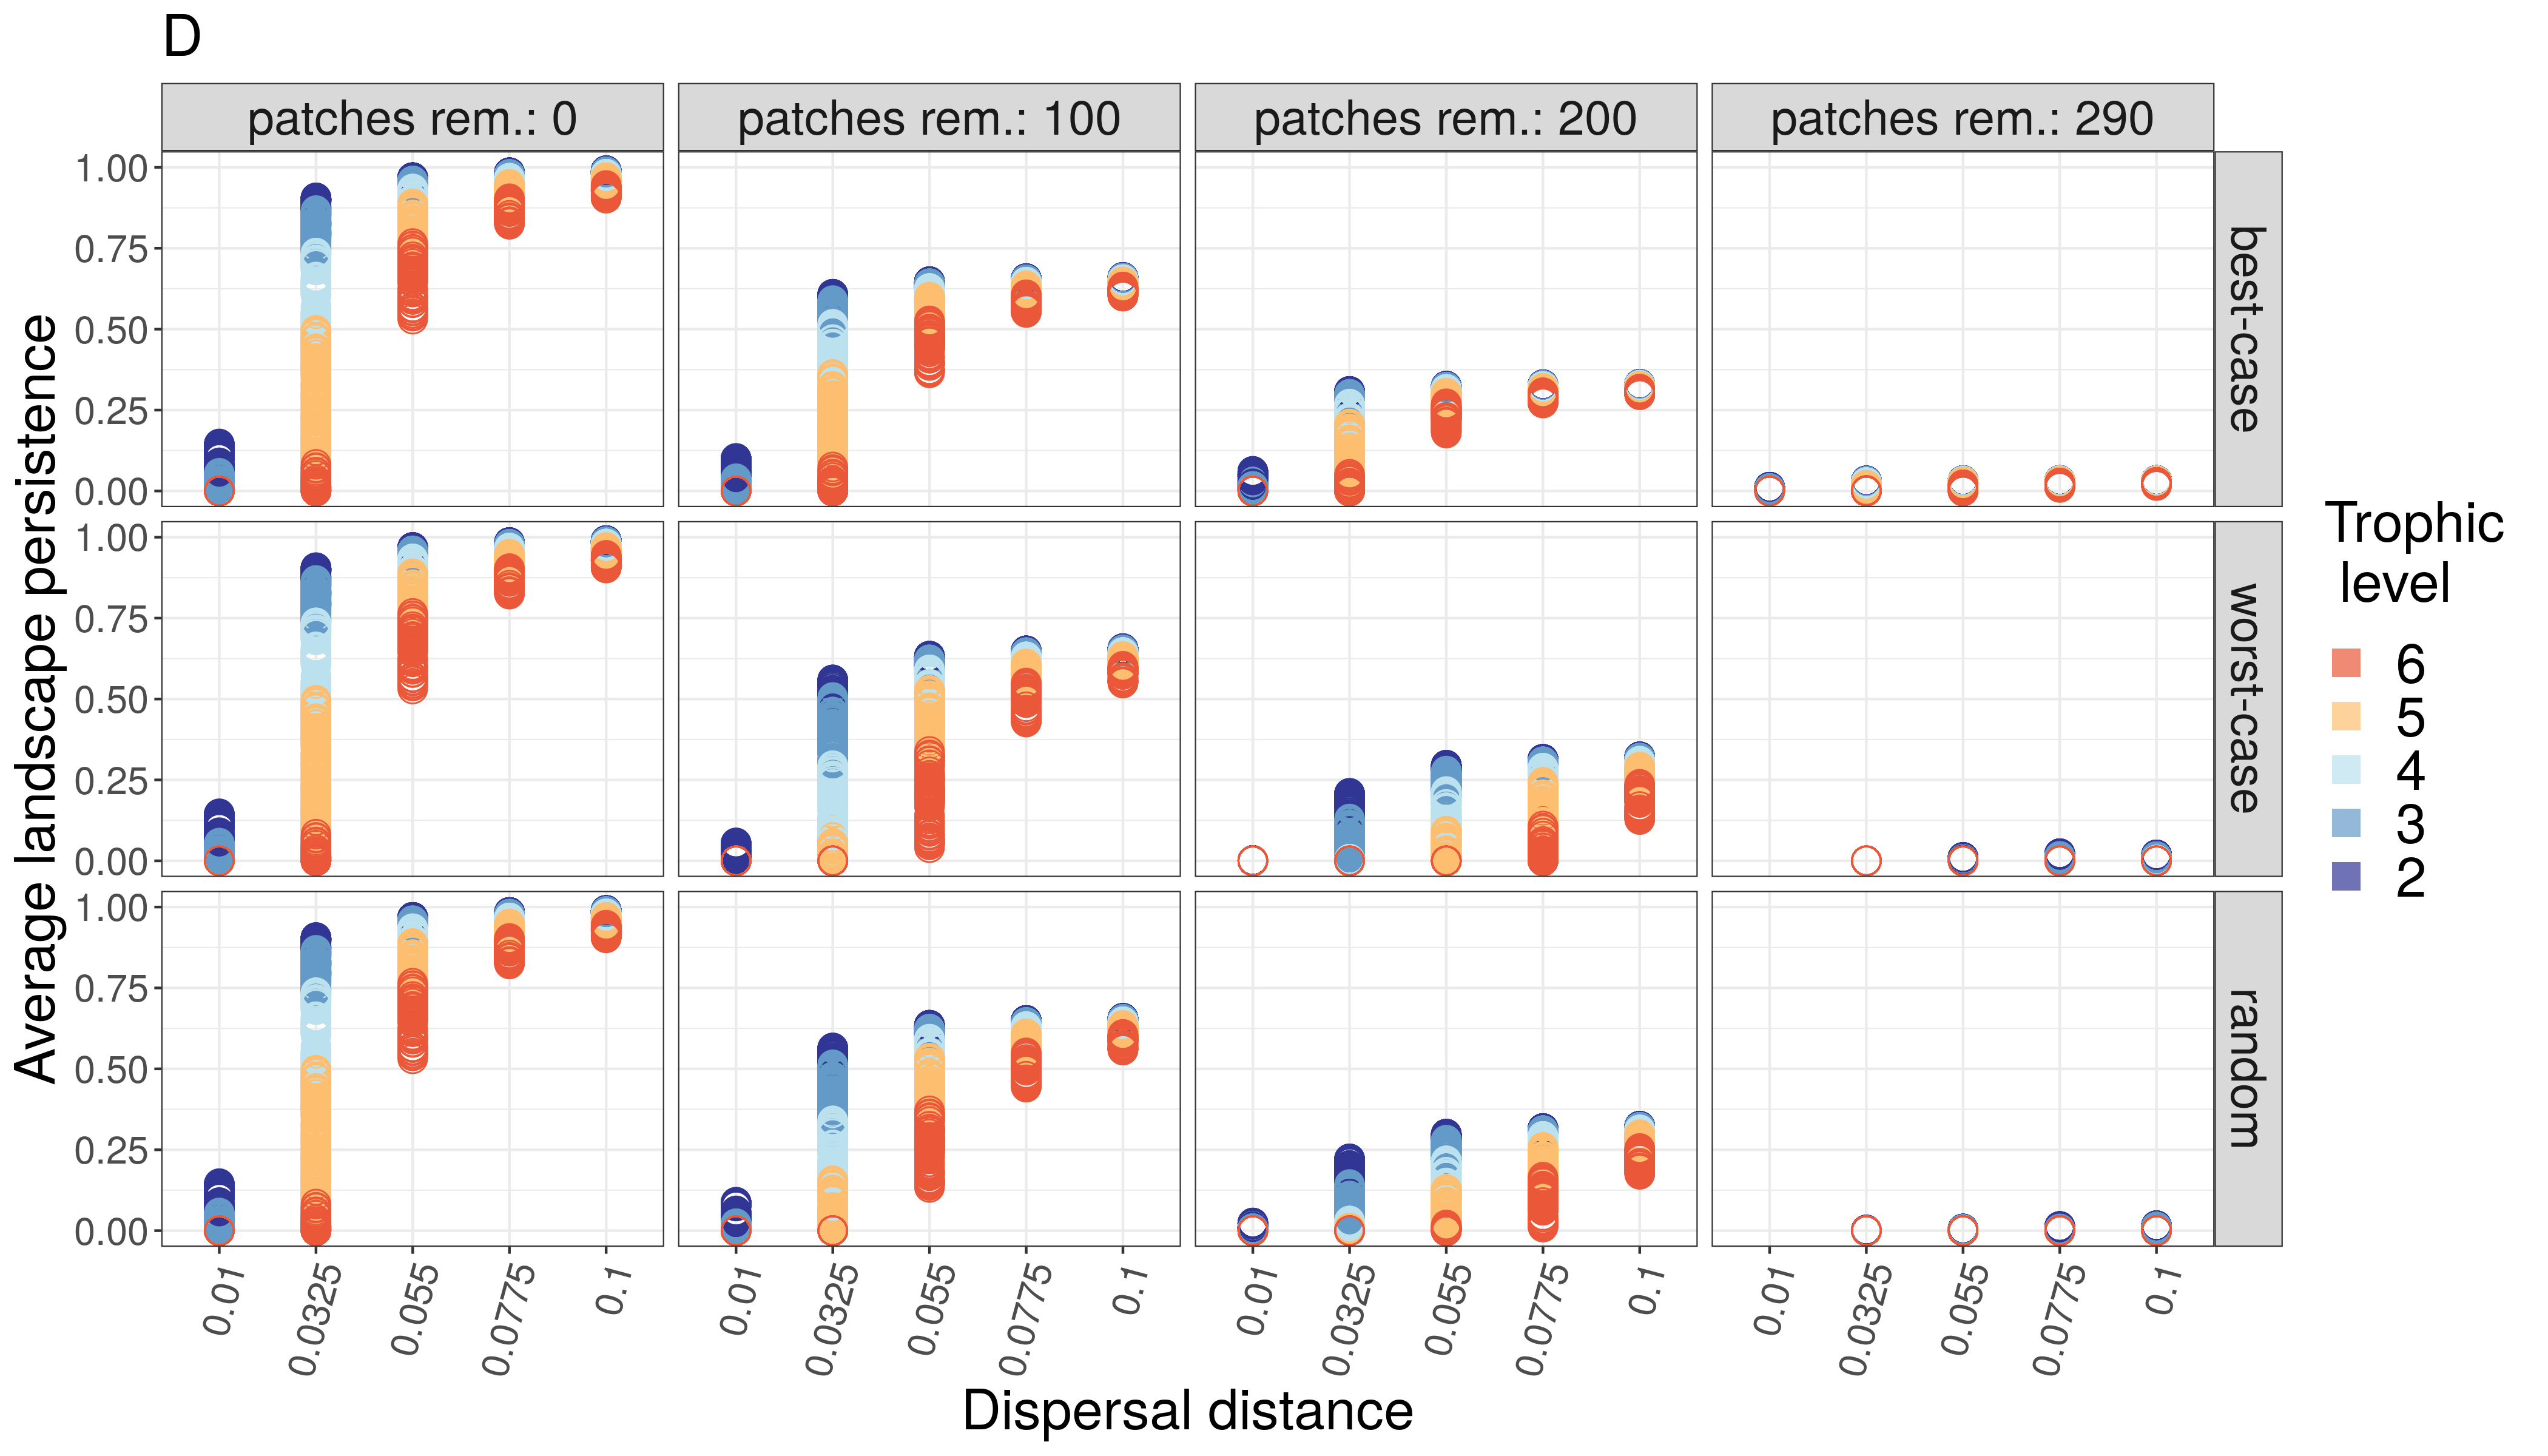
\includegraphics[width=0.8\textwidth,valign=t]{sump_Model_food_web_with_300_consumer_and_100_basal_species_basal_5_5.png}
  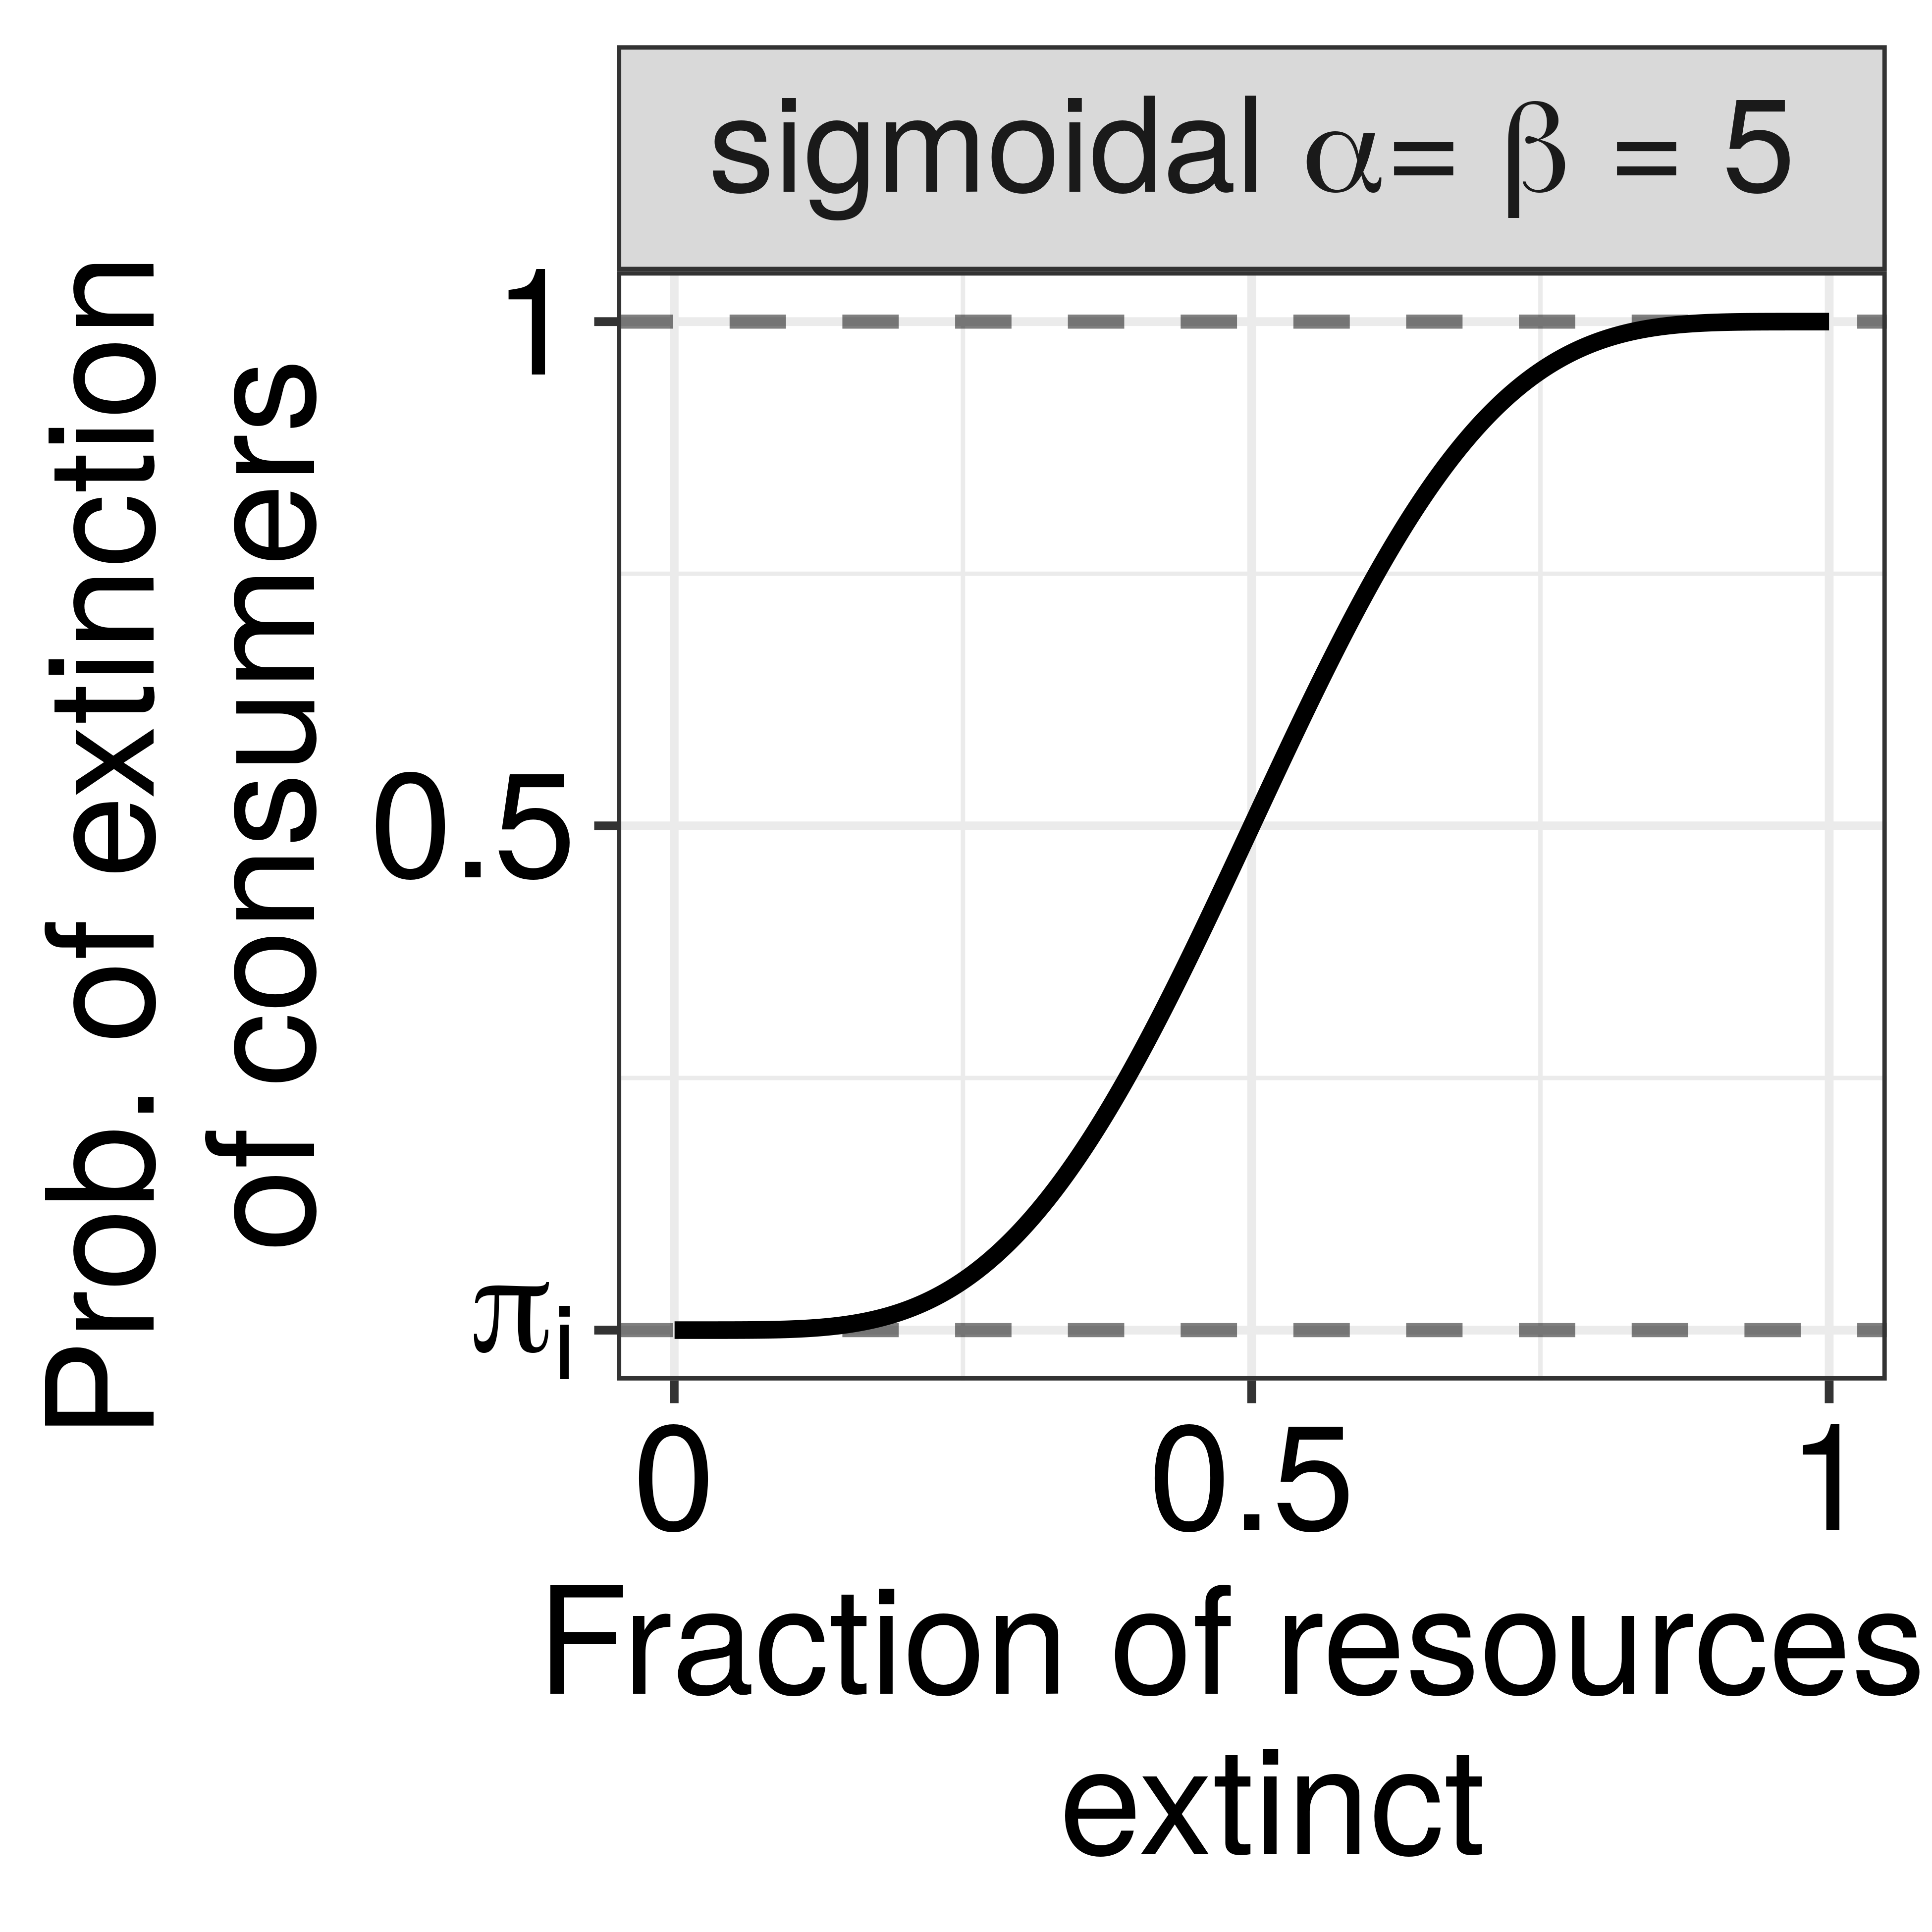
\includegraphics[width=0.19\textwidth,valign=t]{fform_5_5.png}
  \caption{Figure continued.}
  \label{S_fig:patchloss_300_100_distance_2}
\end{figure}

\begin{figure}[!ht]   		   	 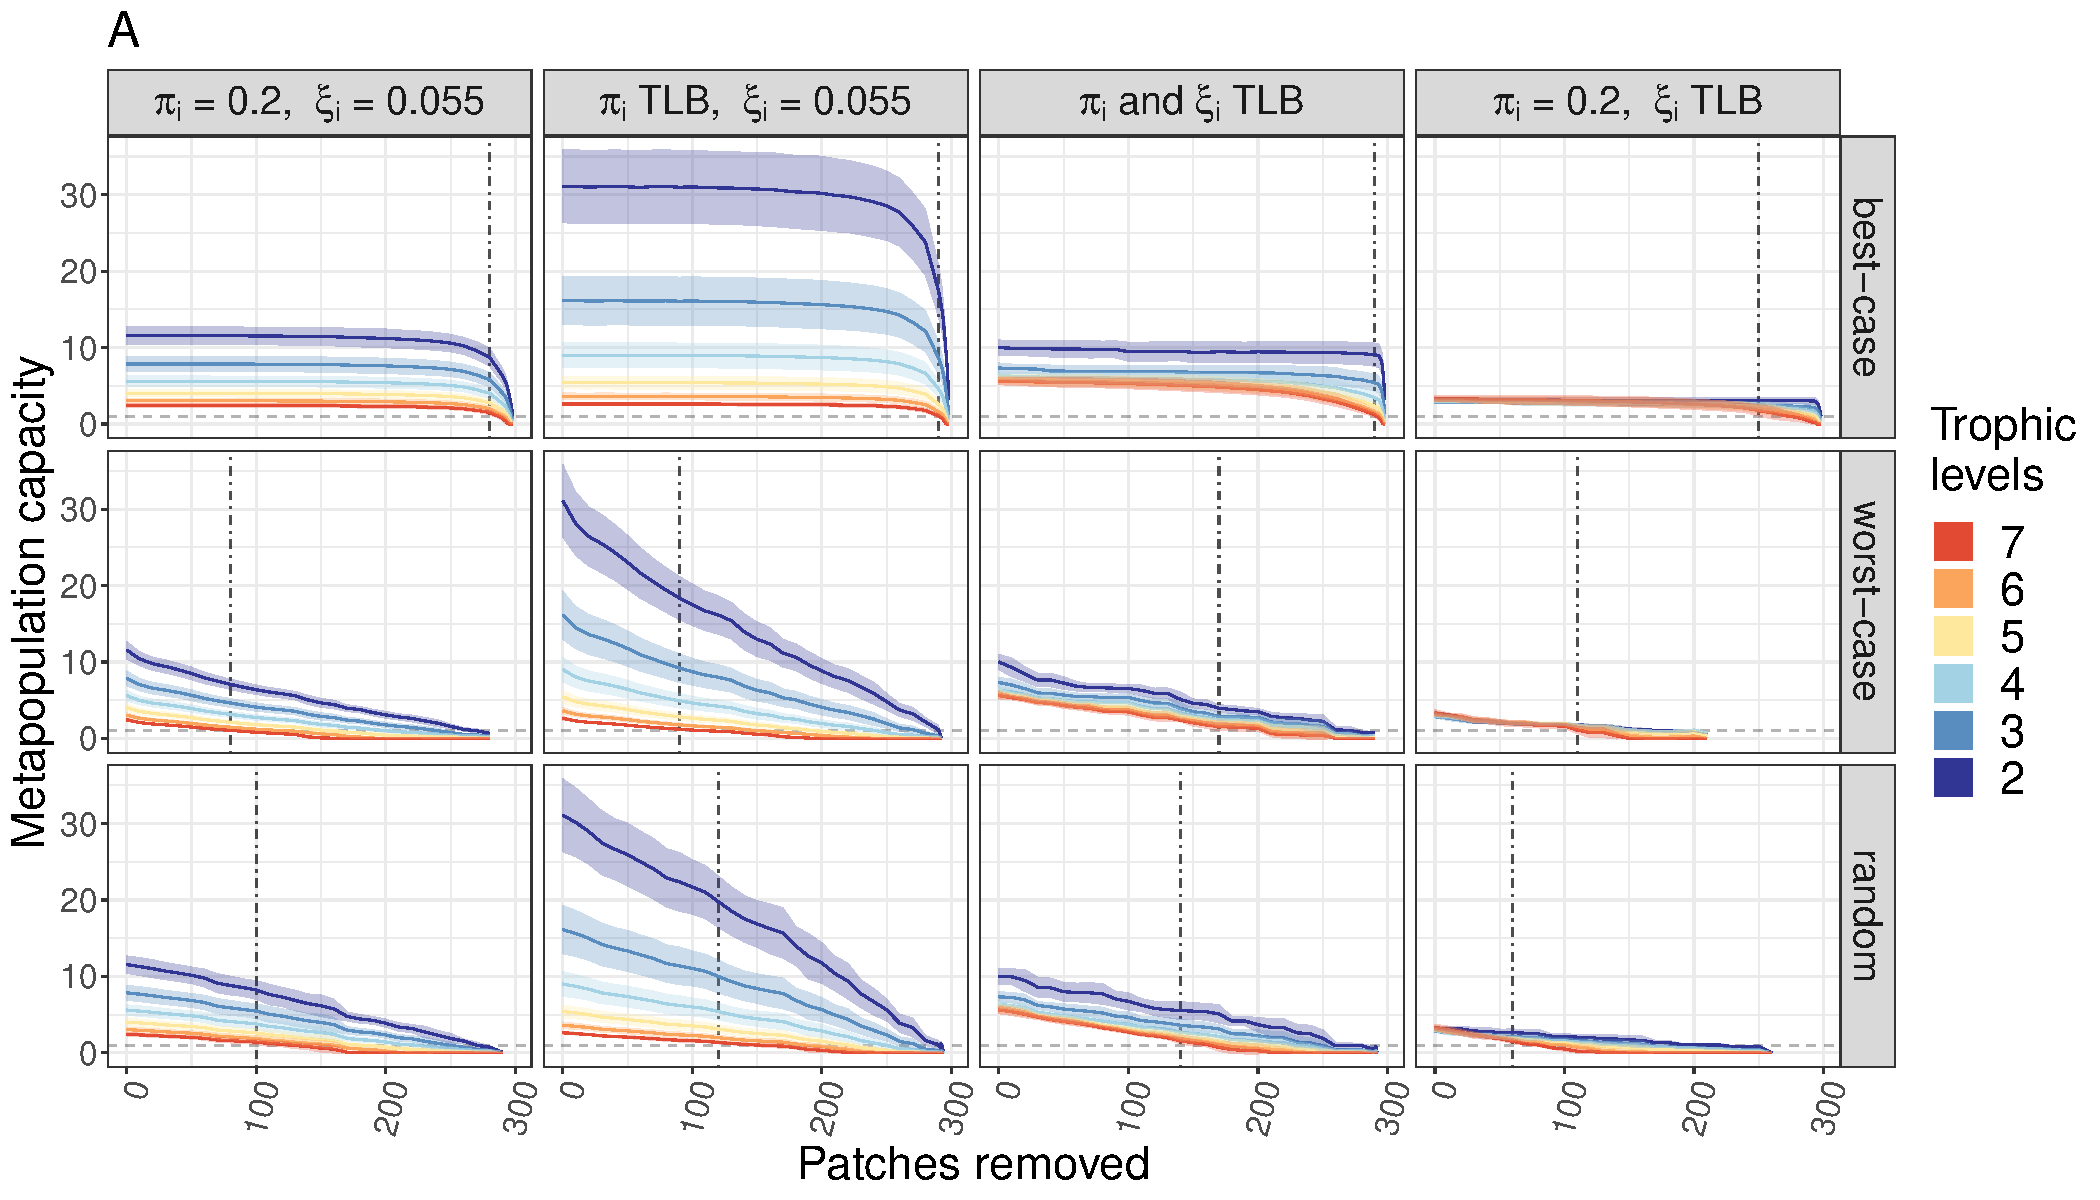
\includegraphics[width=0.8\textwidth,valign=t]{lambda_Model_food_web_with_350_consumer_and_50_basal_species_basal_1_1.pdf}
  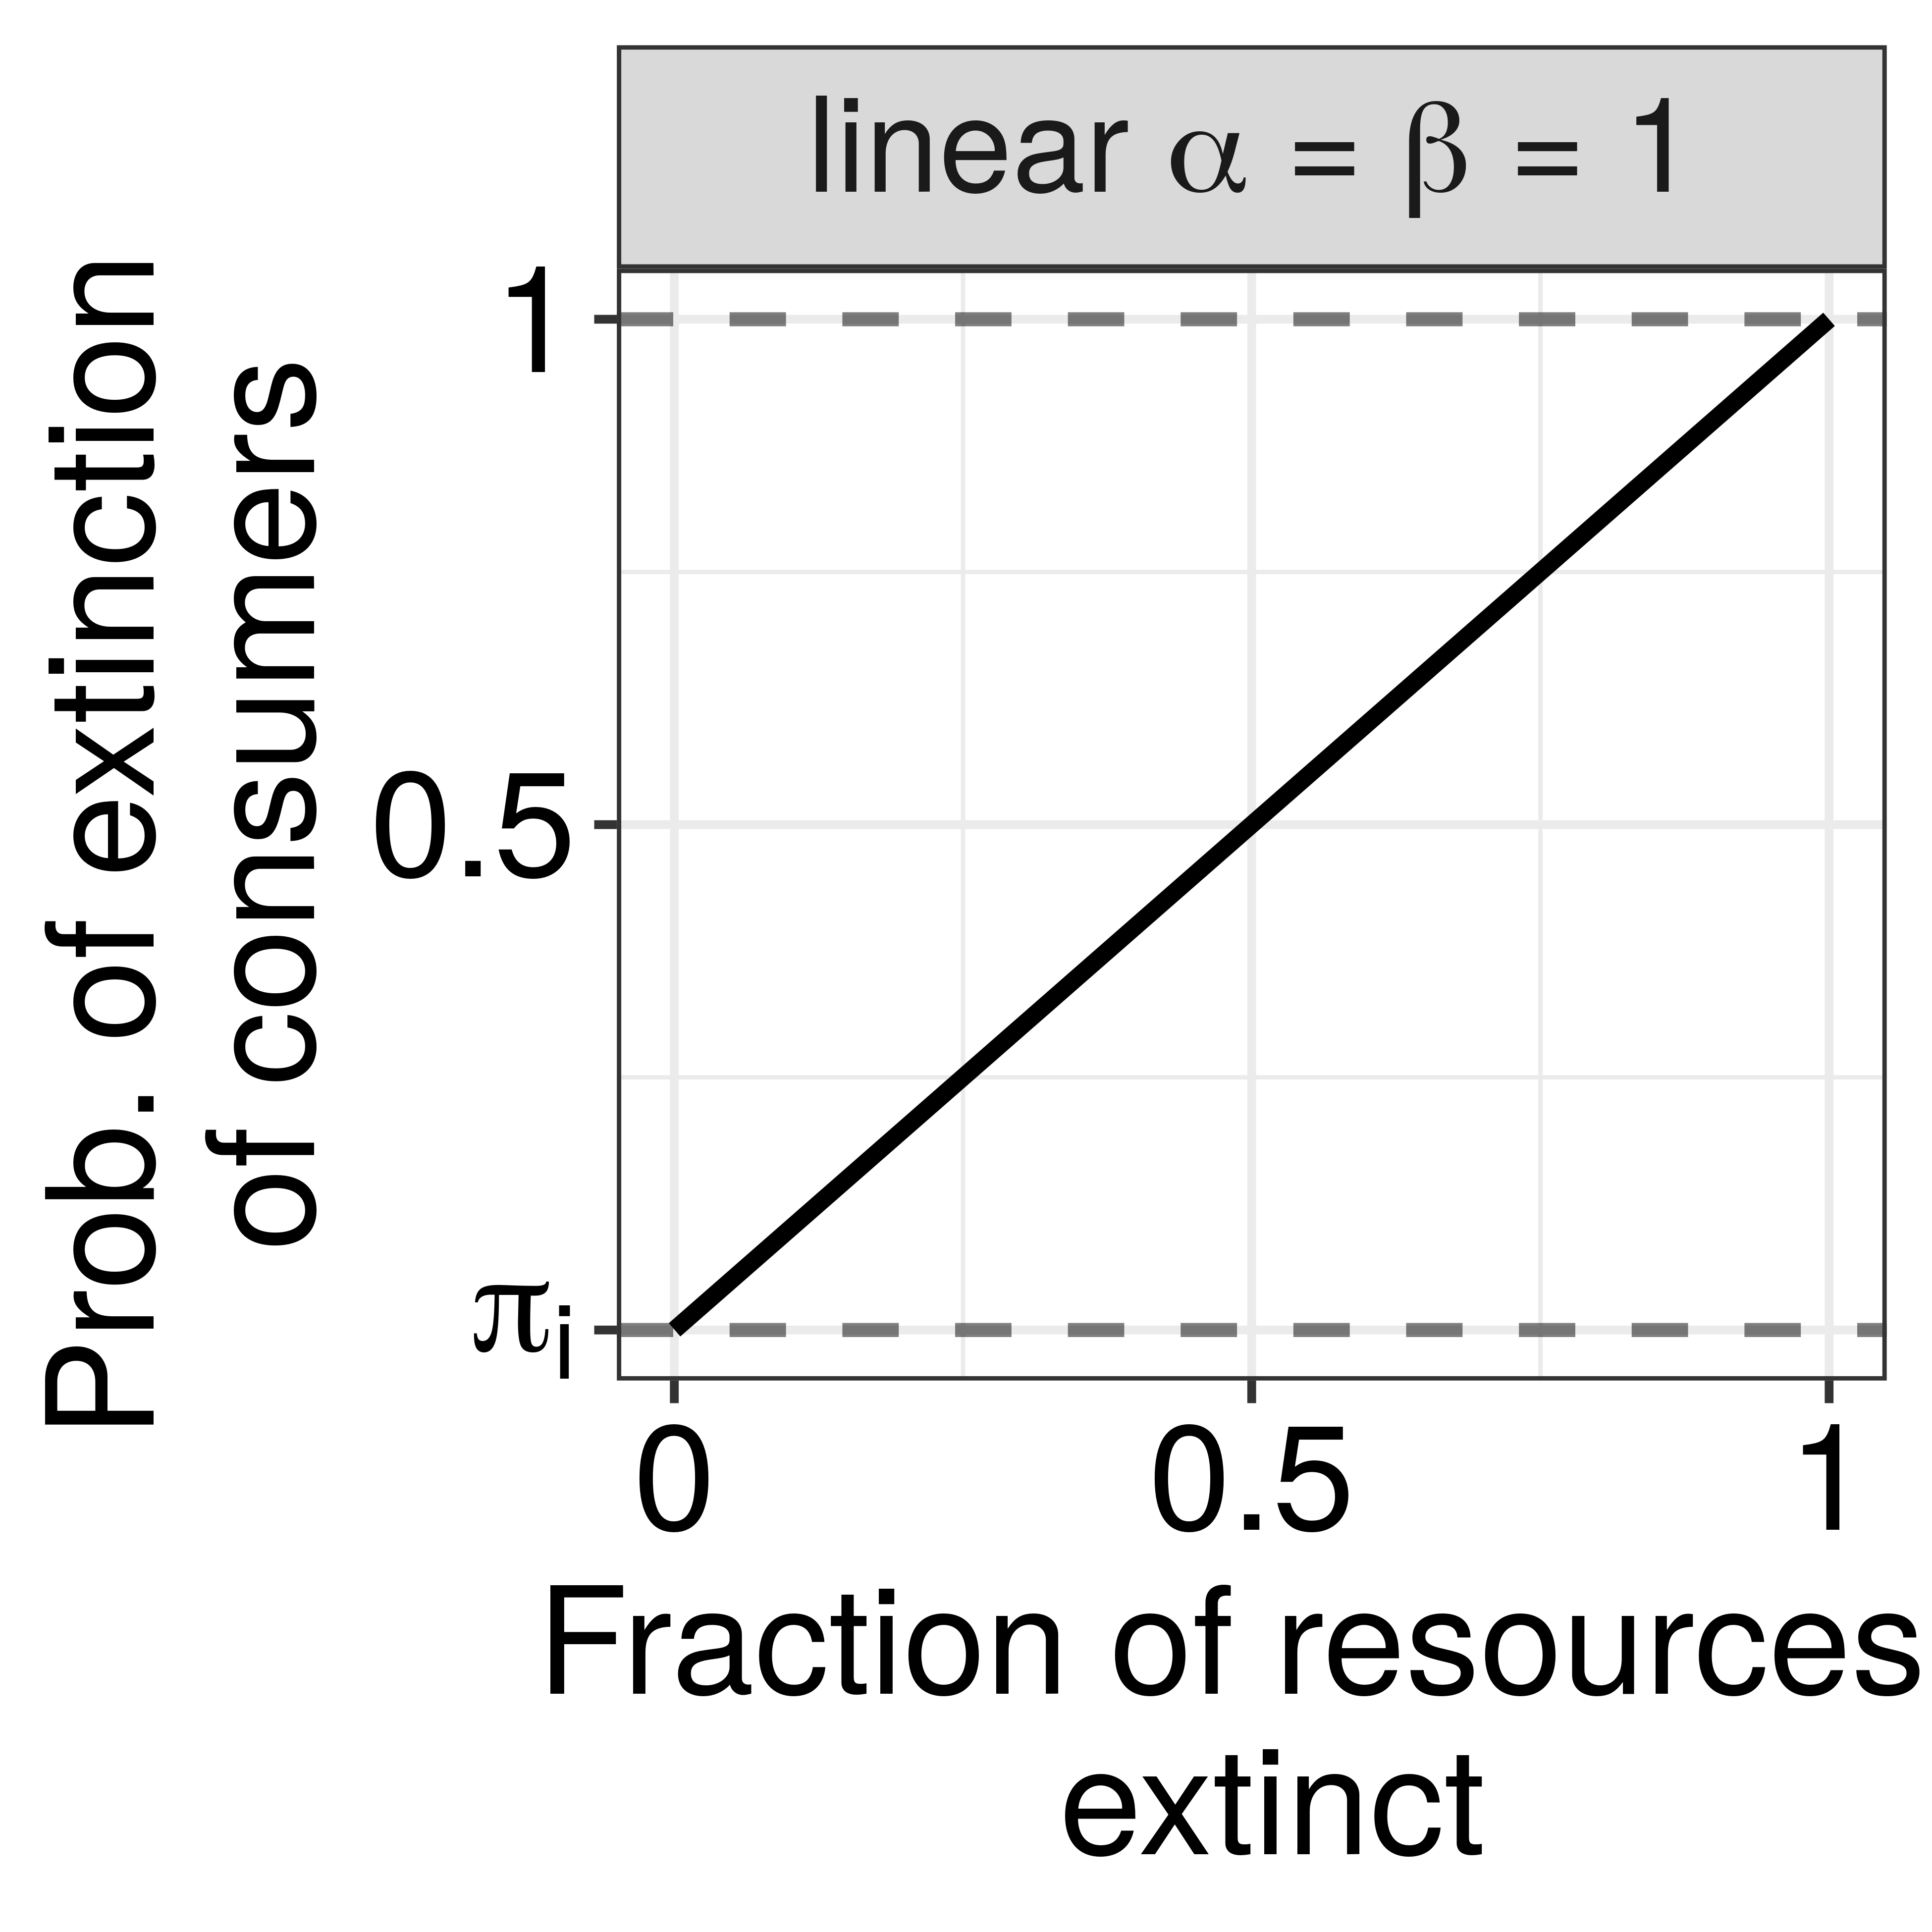
\includegraphics[width=0.19\textwidth,valign=t]{fform_1_1.png}
  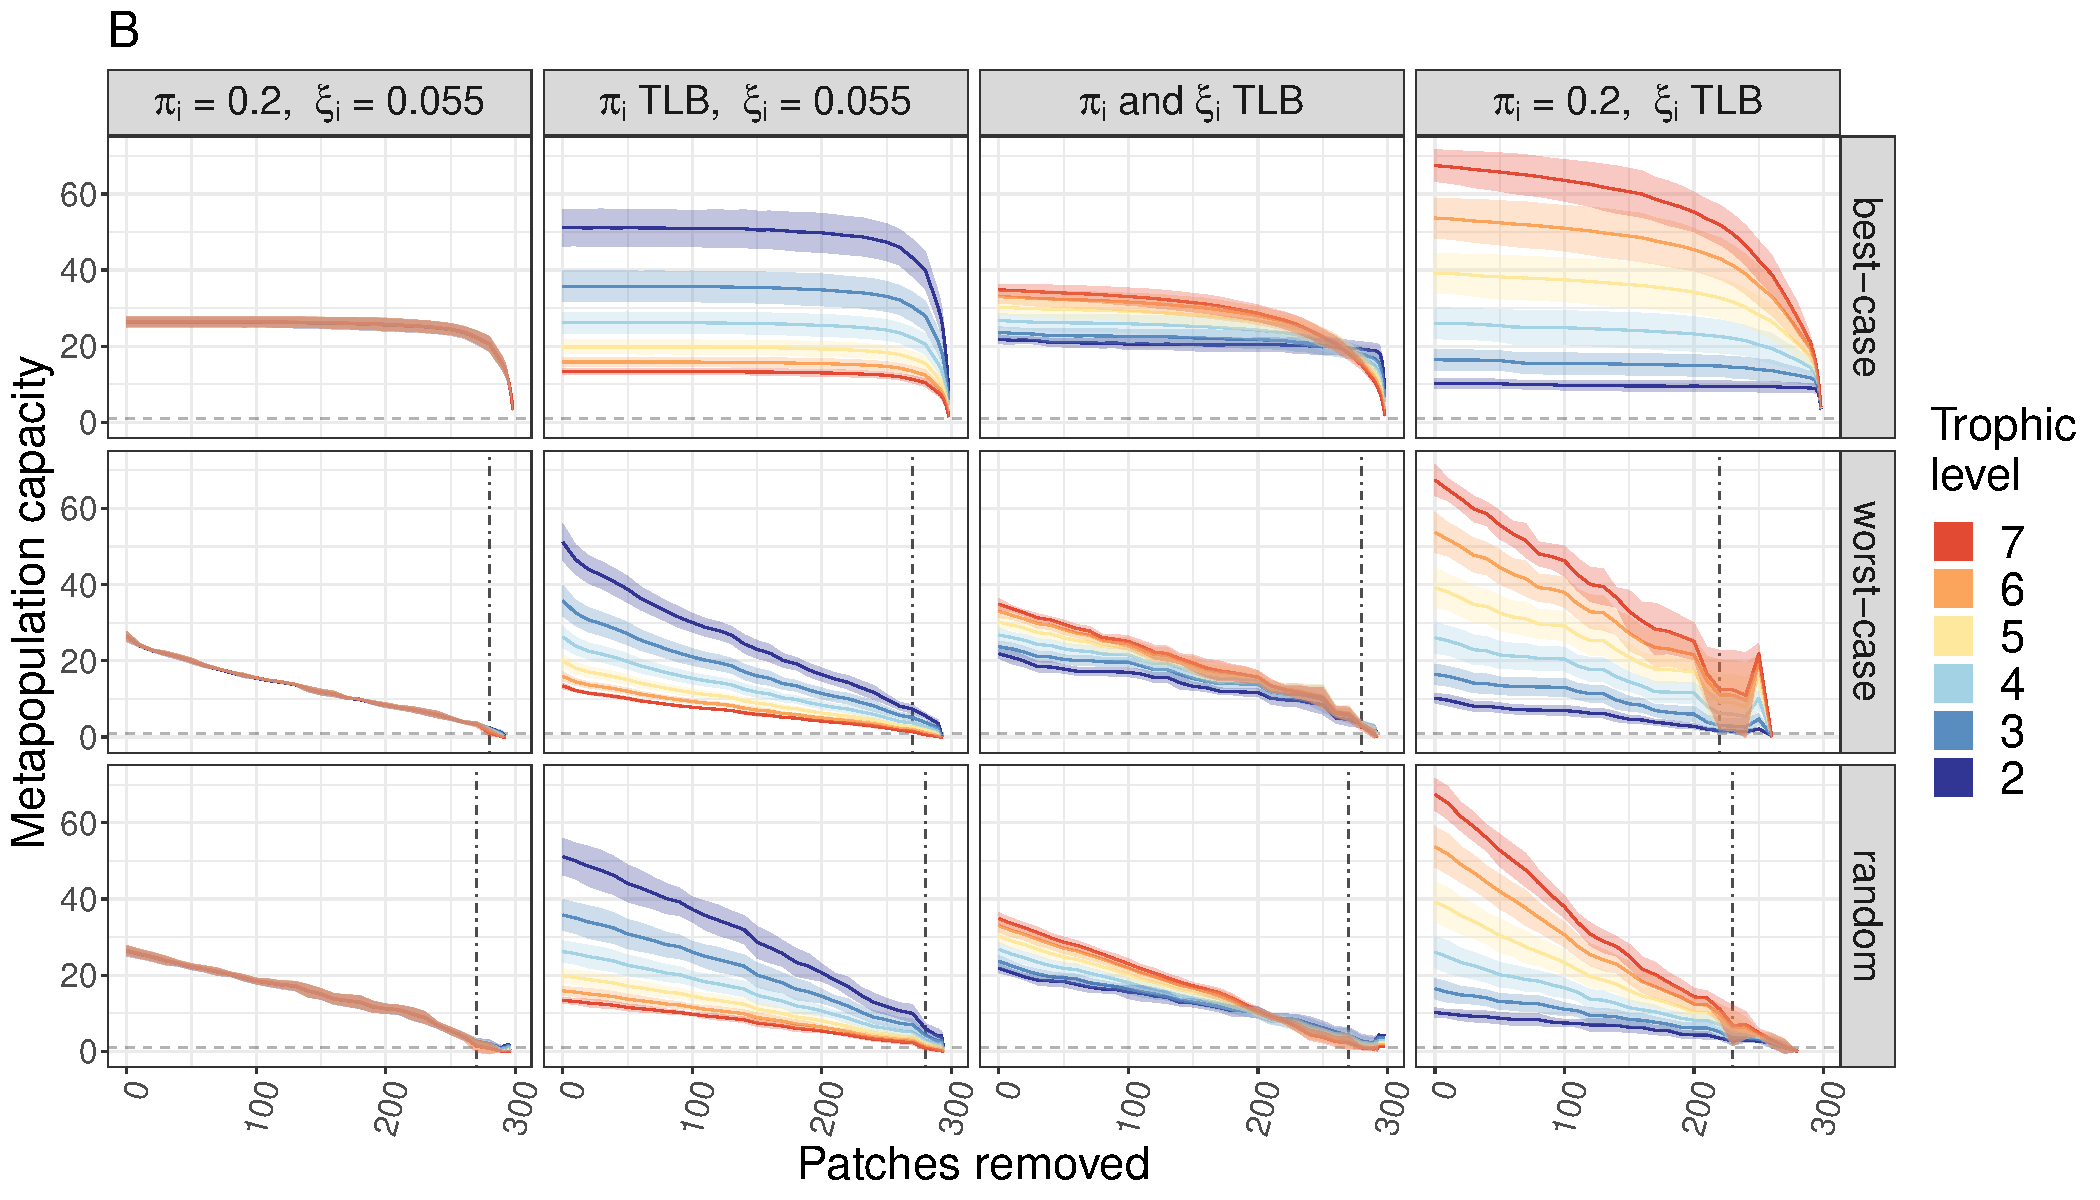
\includegraphics[width=0.8\textwidth,valign=t]{lambda_Model_food_web_with_350_consumer_and_50_basal_species_basal_5_1.pdf}
    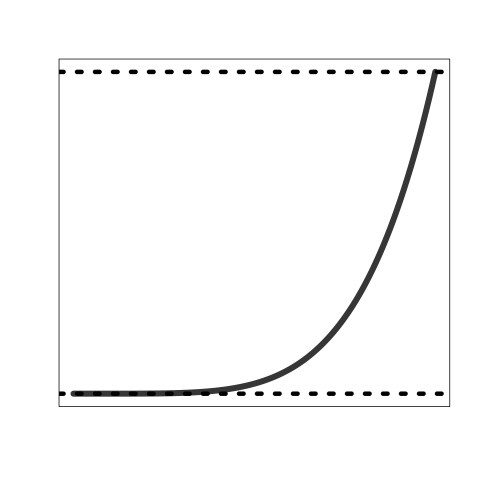
\includegraphics[width=0.19\textwidth,valign=t]{fform_5_1.png}
 \caption{Effect of habitat loss on species persistence in a model food web with 350 consumer and 50 basal species. A-D are for different functional forms of a consumer's response to the loss of resources (top right insets). Species are grouped into trophic levels (color legends); lines show the mean and the bands around them the one standard deviation range of the metapopulation capacities of species in the corresponding trophic level. Rows indicate patch-removal scenario (best-case, worst-case, and random); columns the parameterization method: baseline extinction probabilities $\pi_i$ and dispersal distances $\xi_i$ can either take on one value across all species, or increase with trophic level (trophic level-based, TLB). Horizontal dashed lines highlight a metapopulation capacity of $1$, the threshold for long-term species persistence. Vertical dashed lines show when the metapopulation capacity of the top species in the food web drops below this threshold.}
 \label{S_fig:patchloss_350_50_1}
\end{figure}

\begin{figure}\ContinuedFloat
 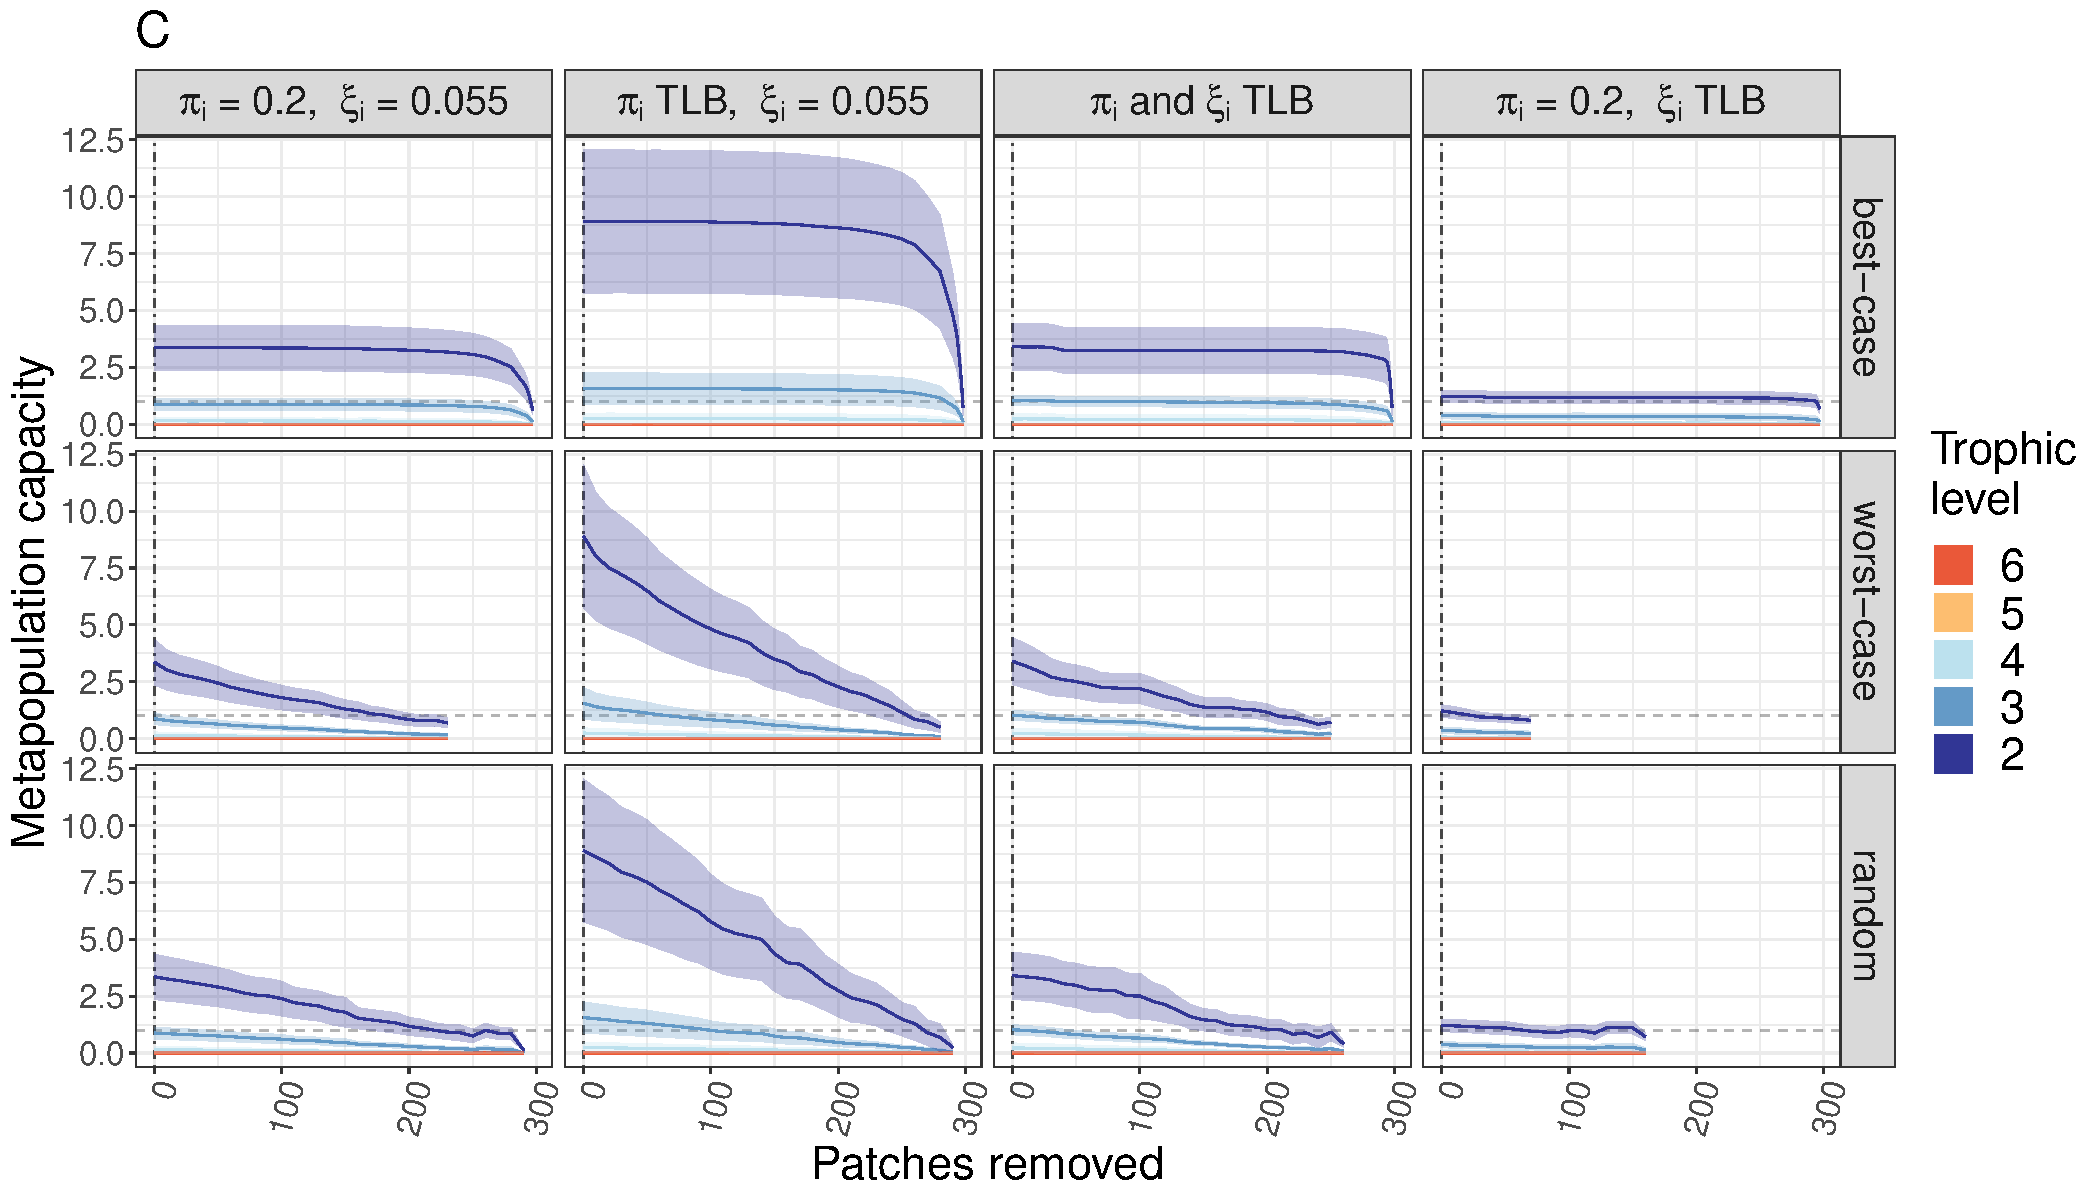
\includegraphics[width=0.8\textwidth,valign=t]{lambda_Model_food_web_with_300_consumer_and_100_basal_species_basal_1_5.pdf}
  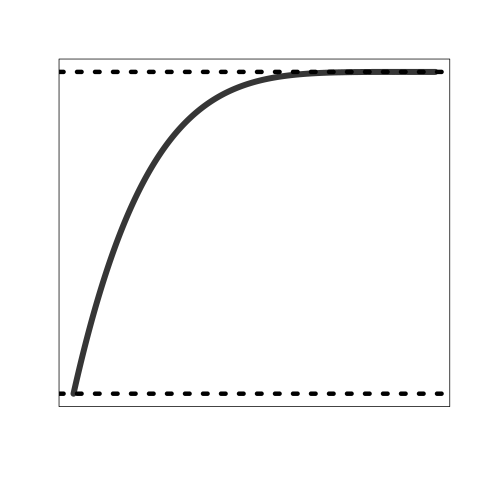
\includegraphics[width=0.19\textwidth,valign=t]{fform_1_5.png}
  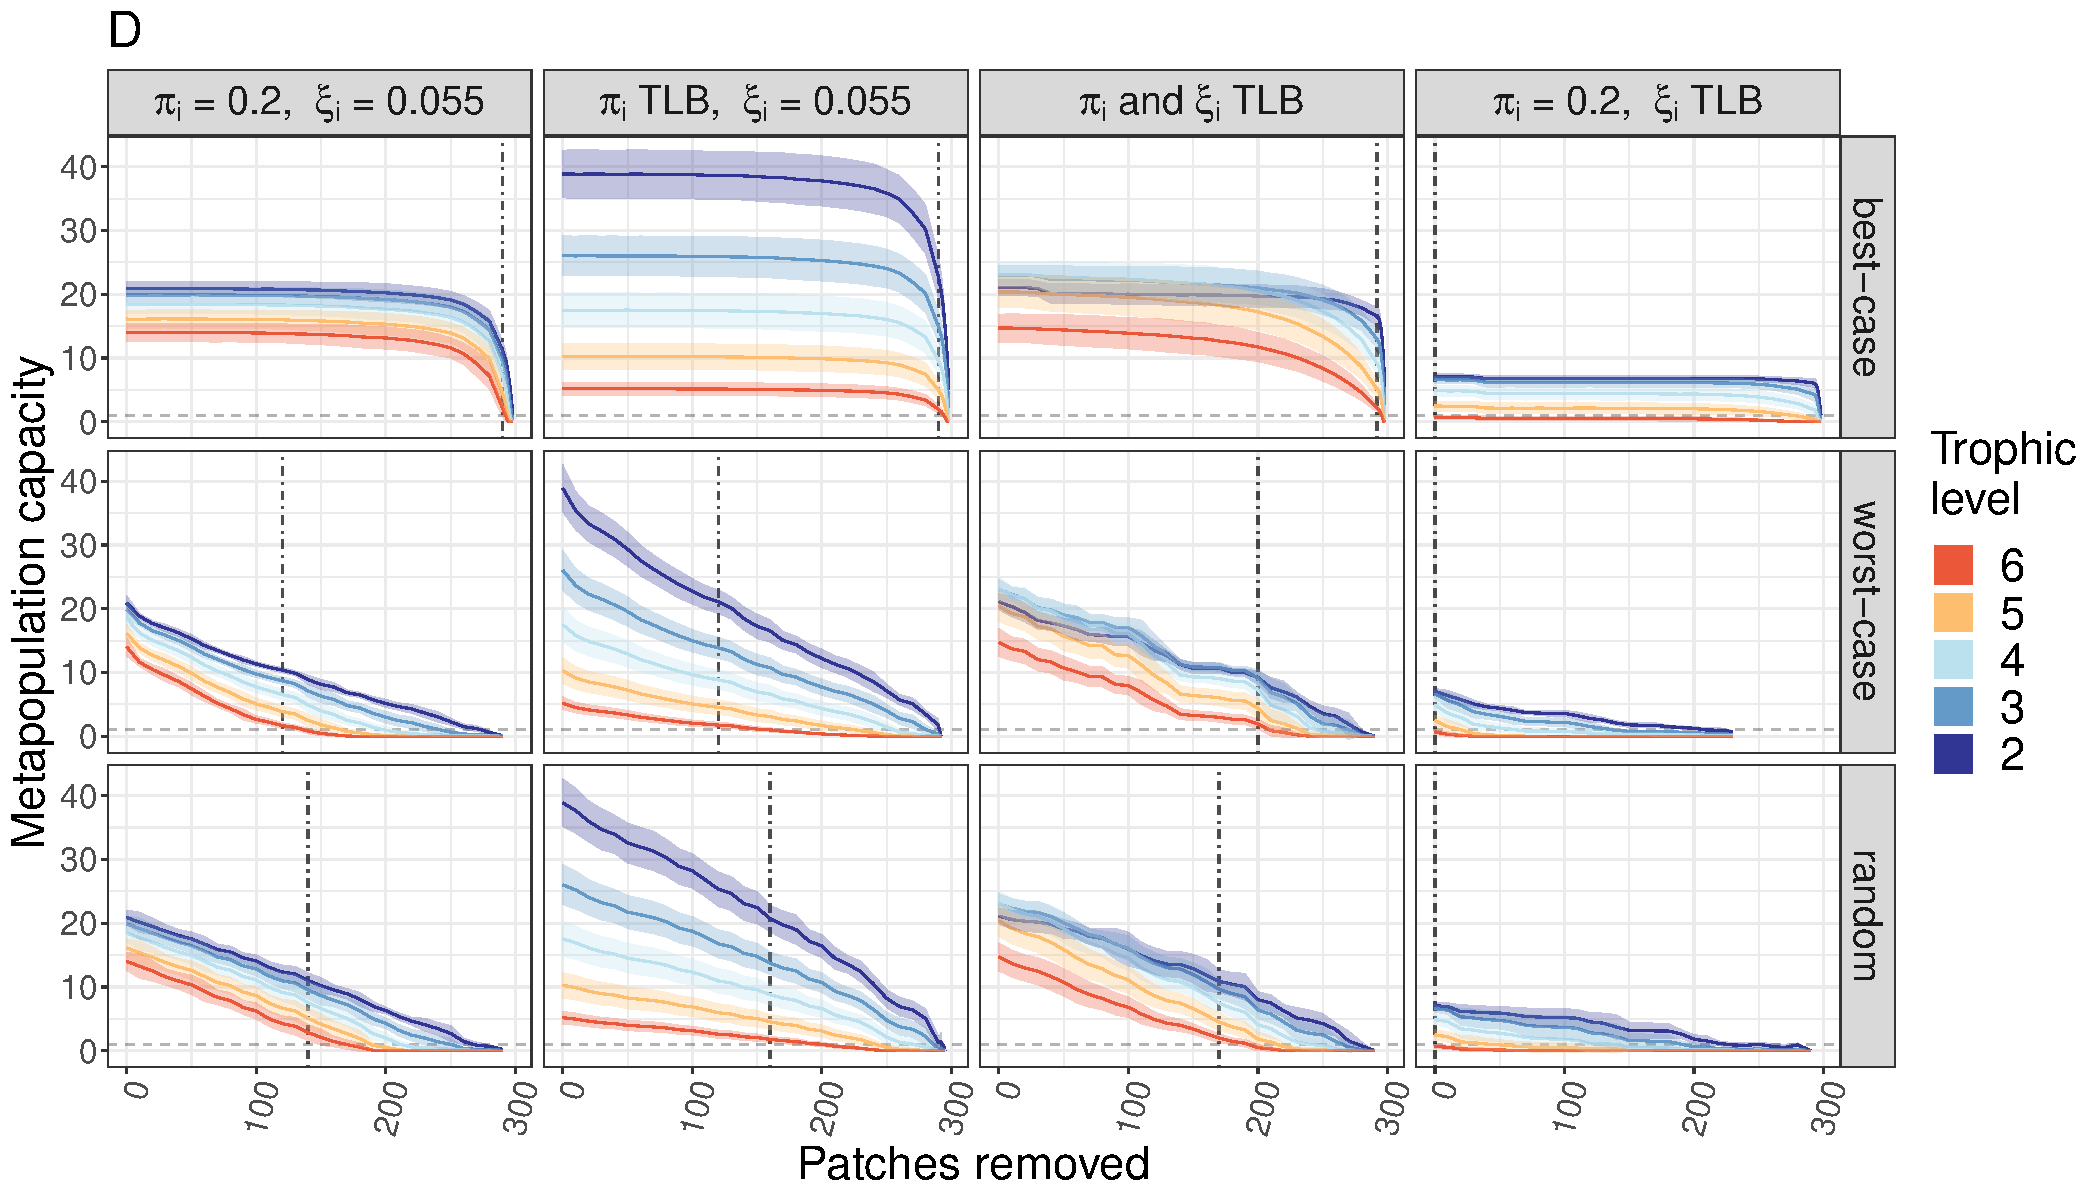
\includegraphics[width=0.8\textwidth,valign=t]{lambda_Model_food_web_with_300_consumer_and_100_basal_species_basal_5_5.pdf}
  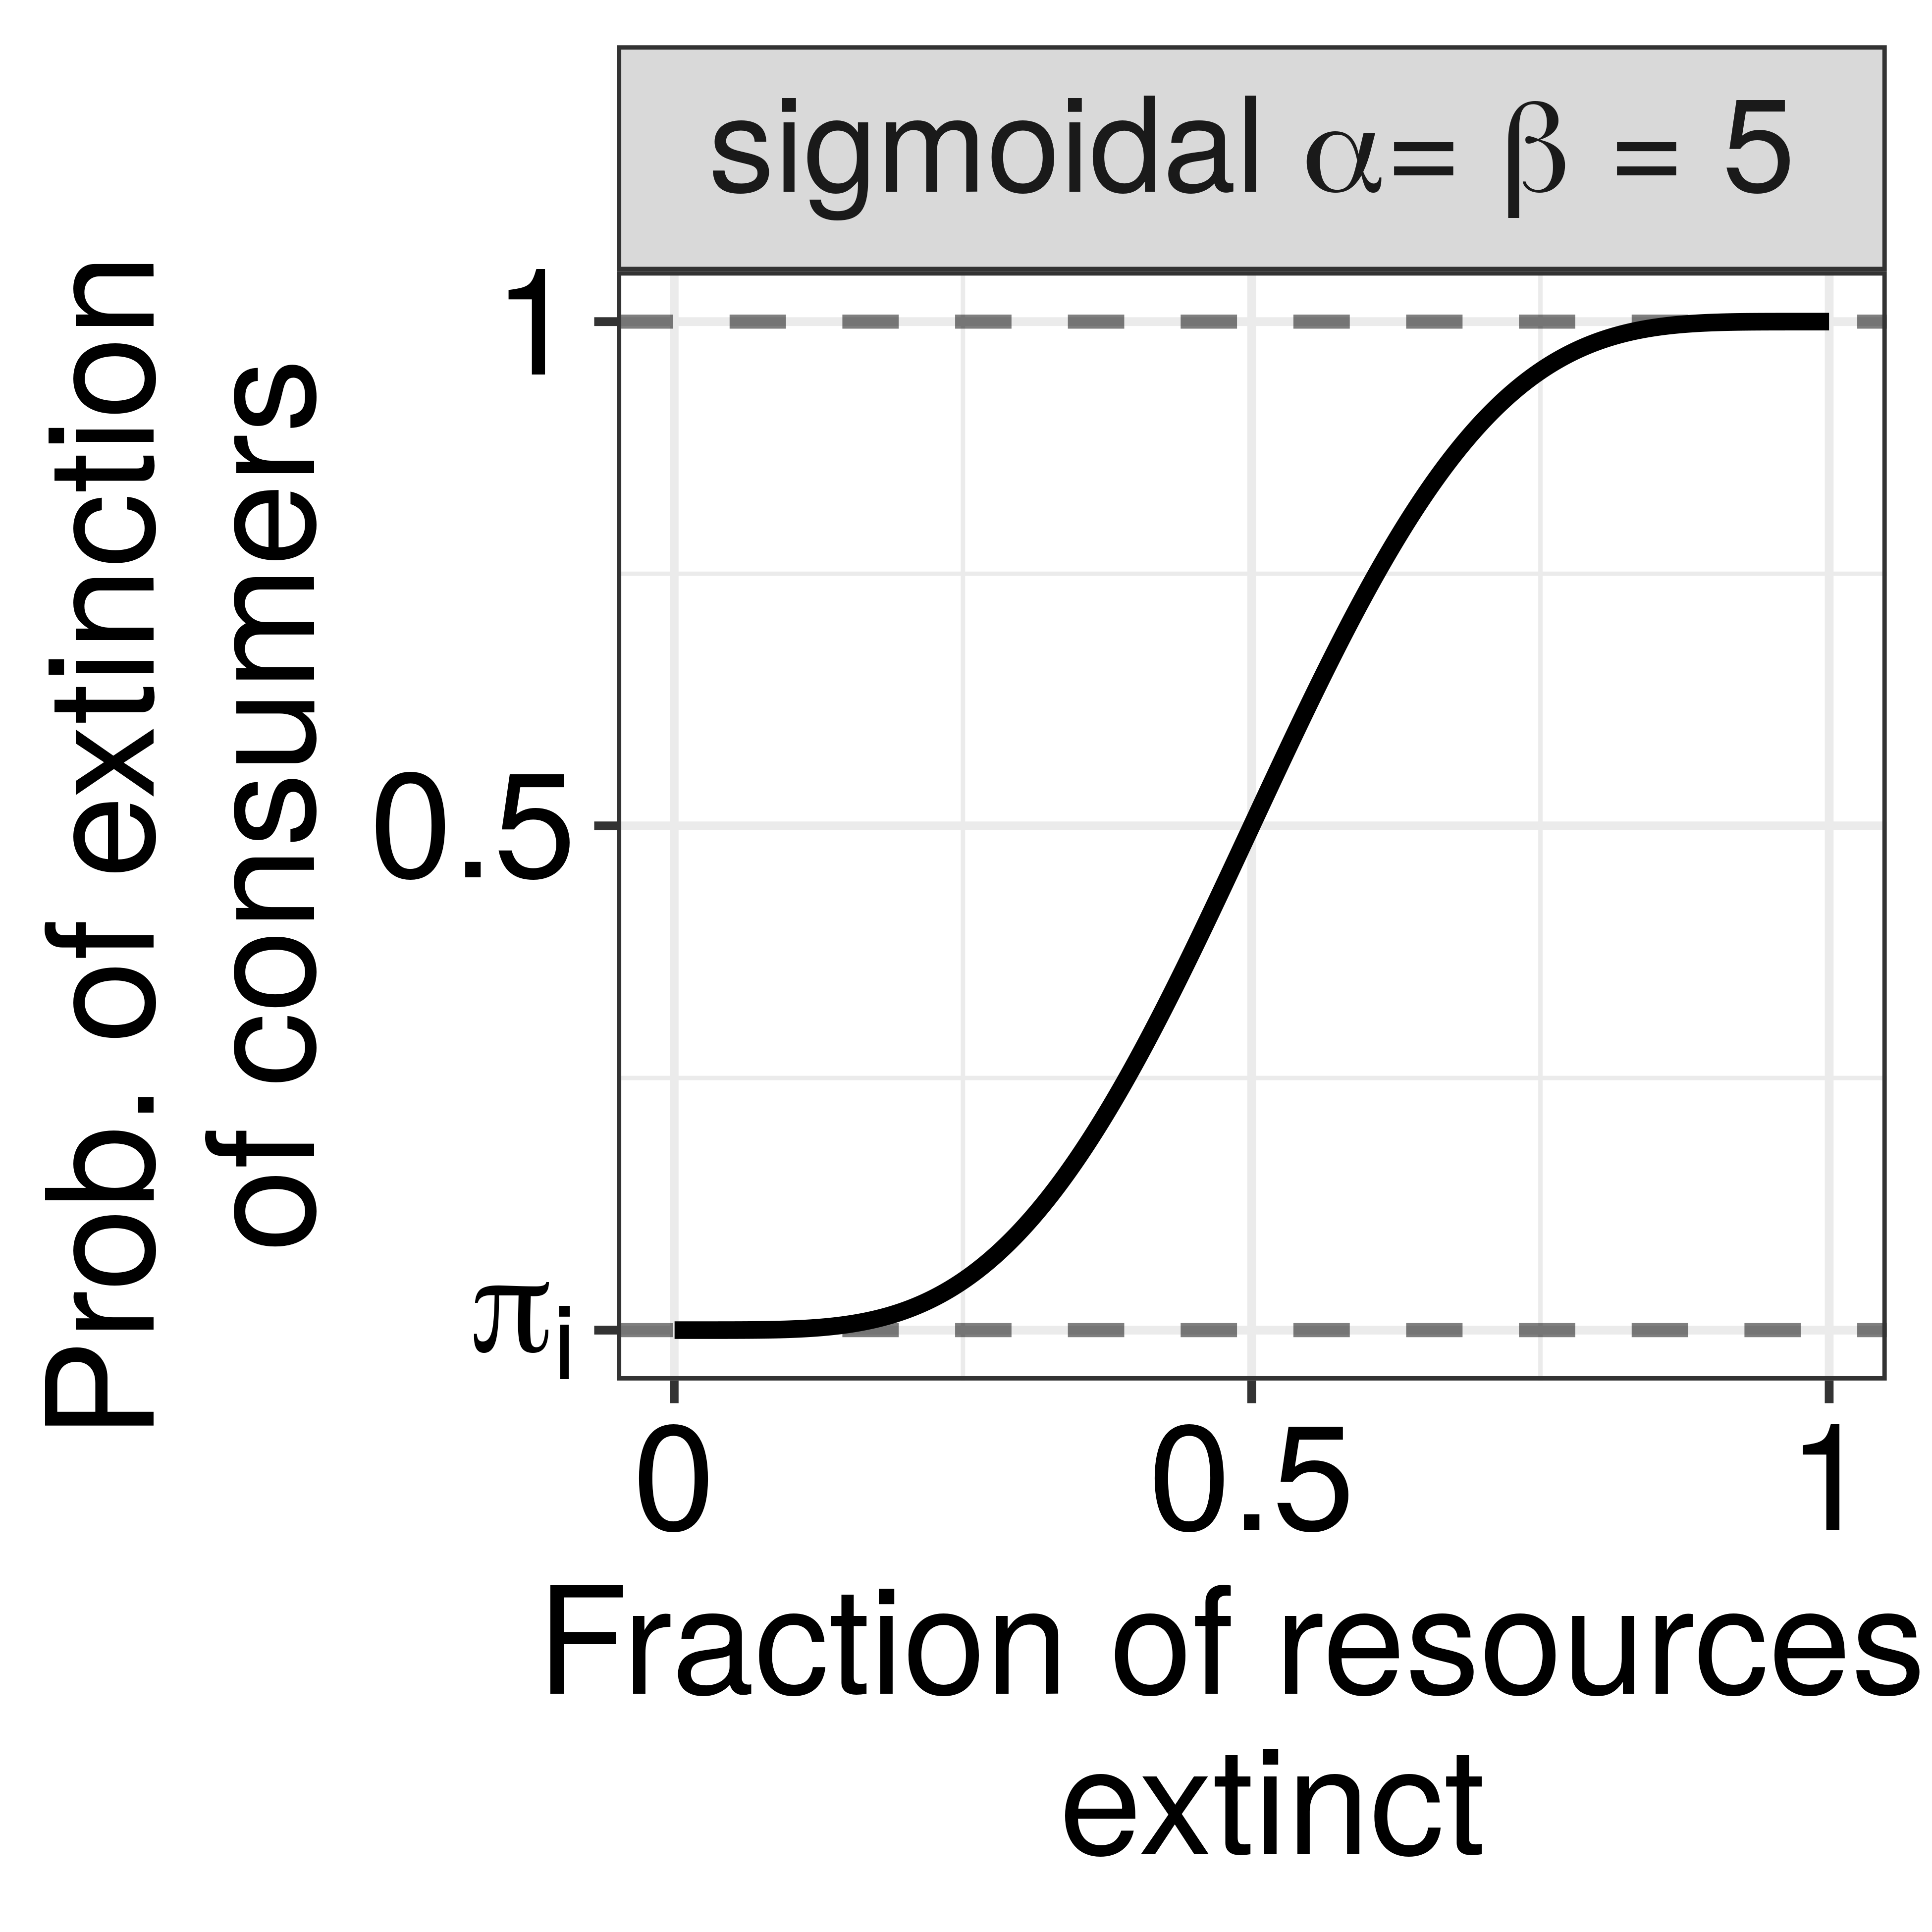
\includegraphics[width=0.19\textwidth,valign=t]{fform_5_5.png}
 \caption{Figure continued.}
 \label{S_fig:patchloss_350_50_2}
\end{figure}

\begin{figure}
  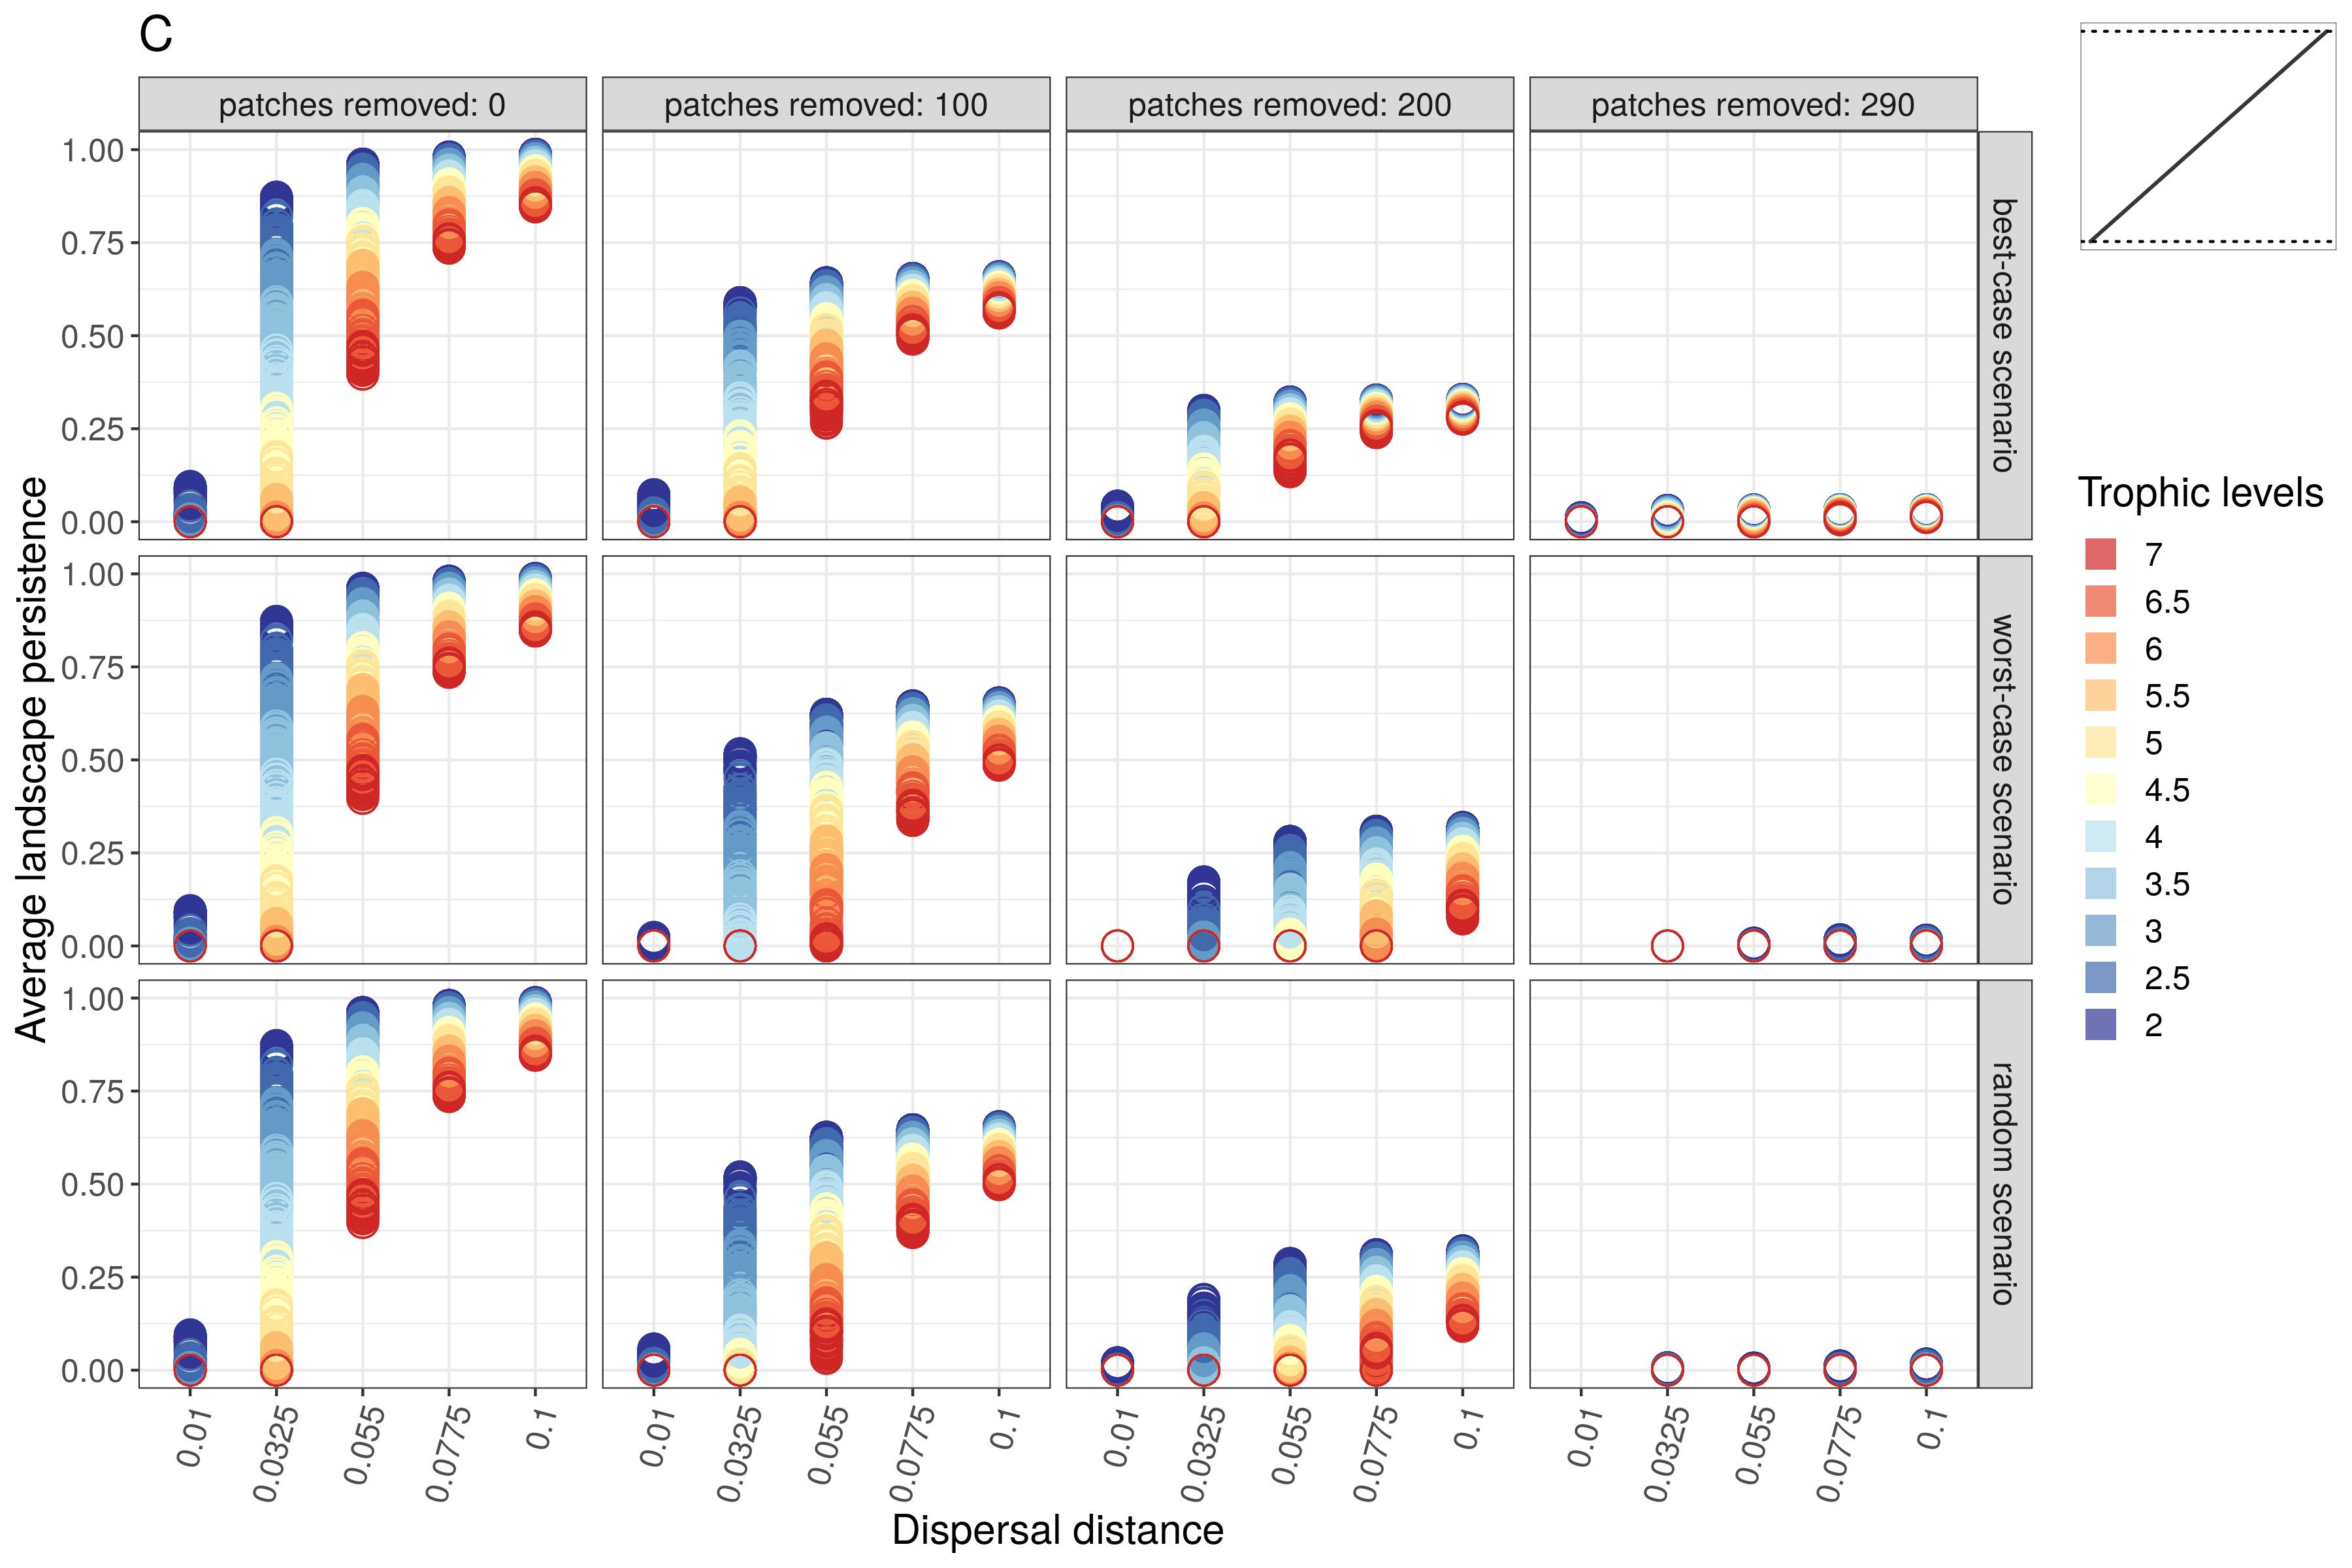
\includegraphics[width=0.8\textwidth,valign=t]{sump_Model_food_web_with_350_consumer_and_50_basal_species_basal_1_1.png}
  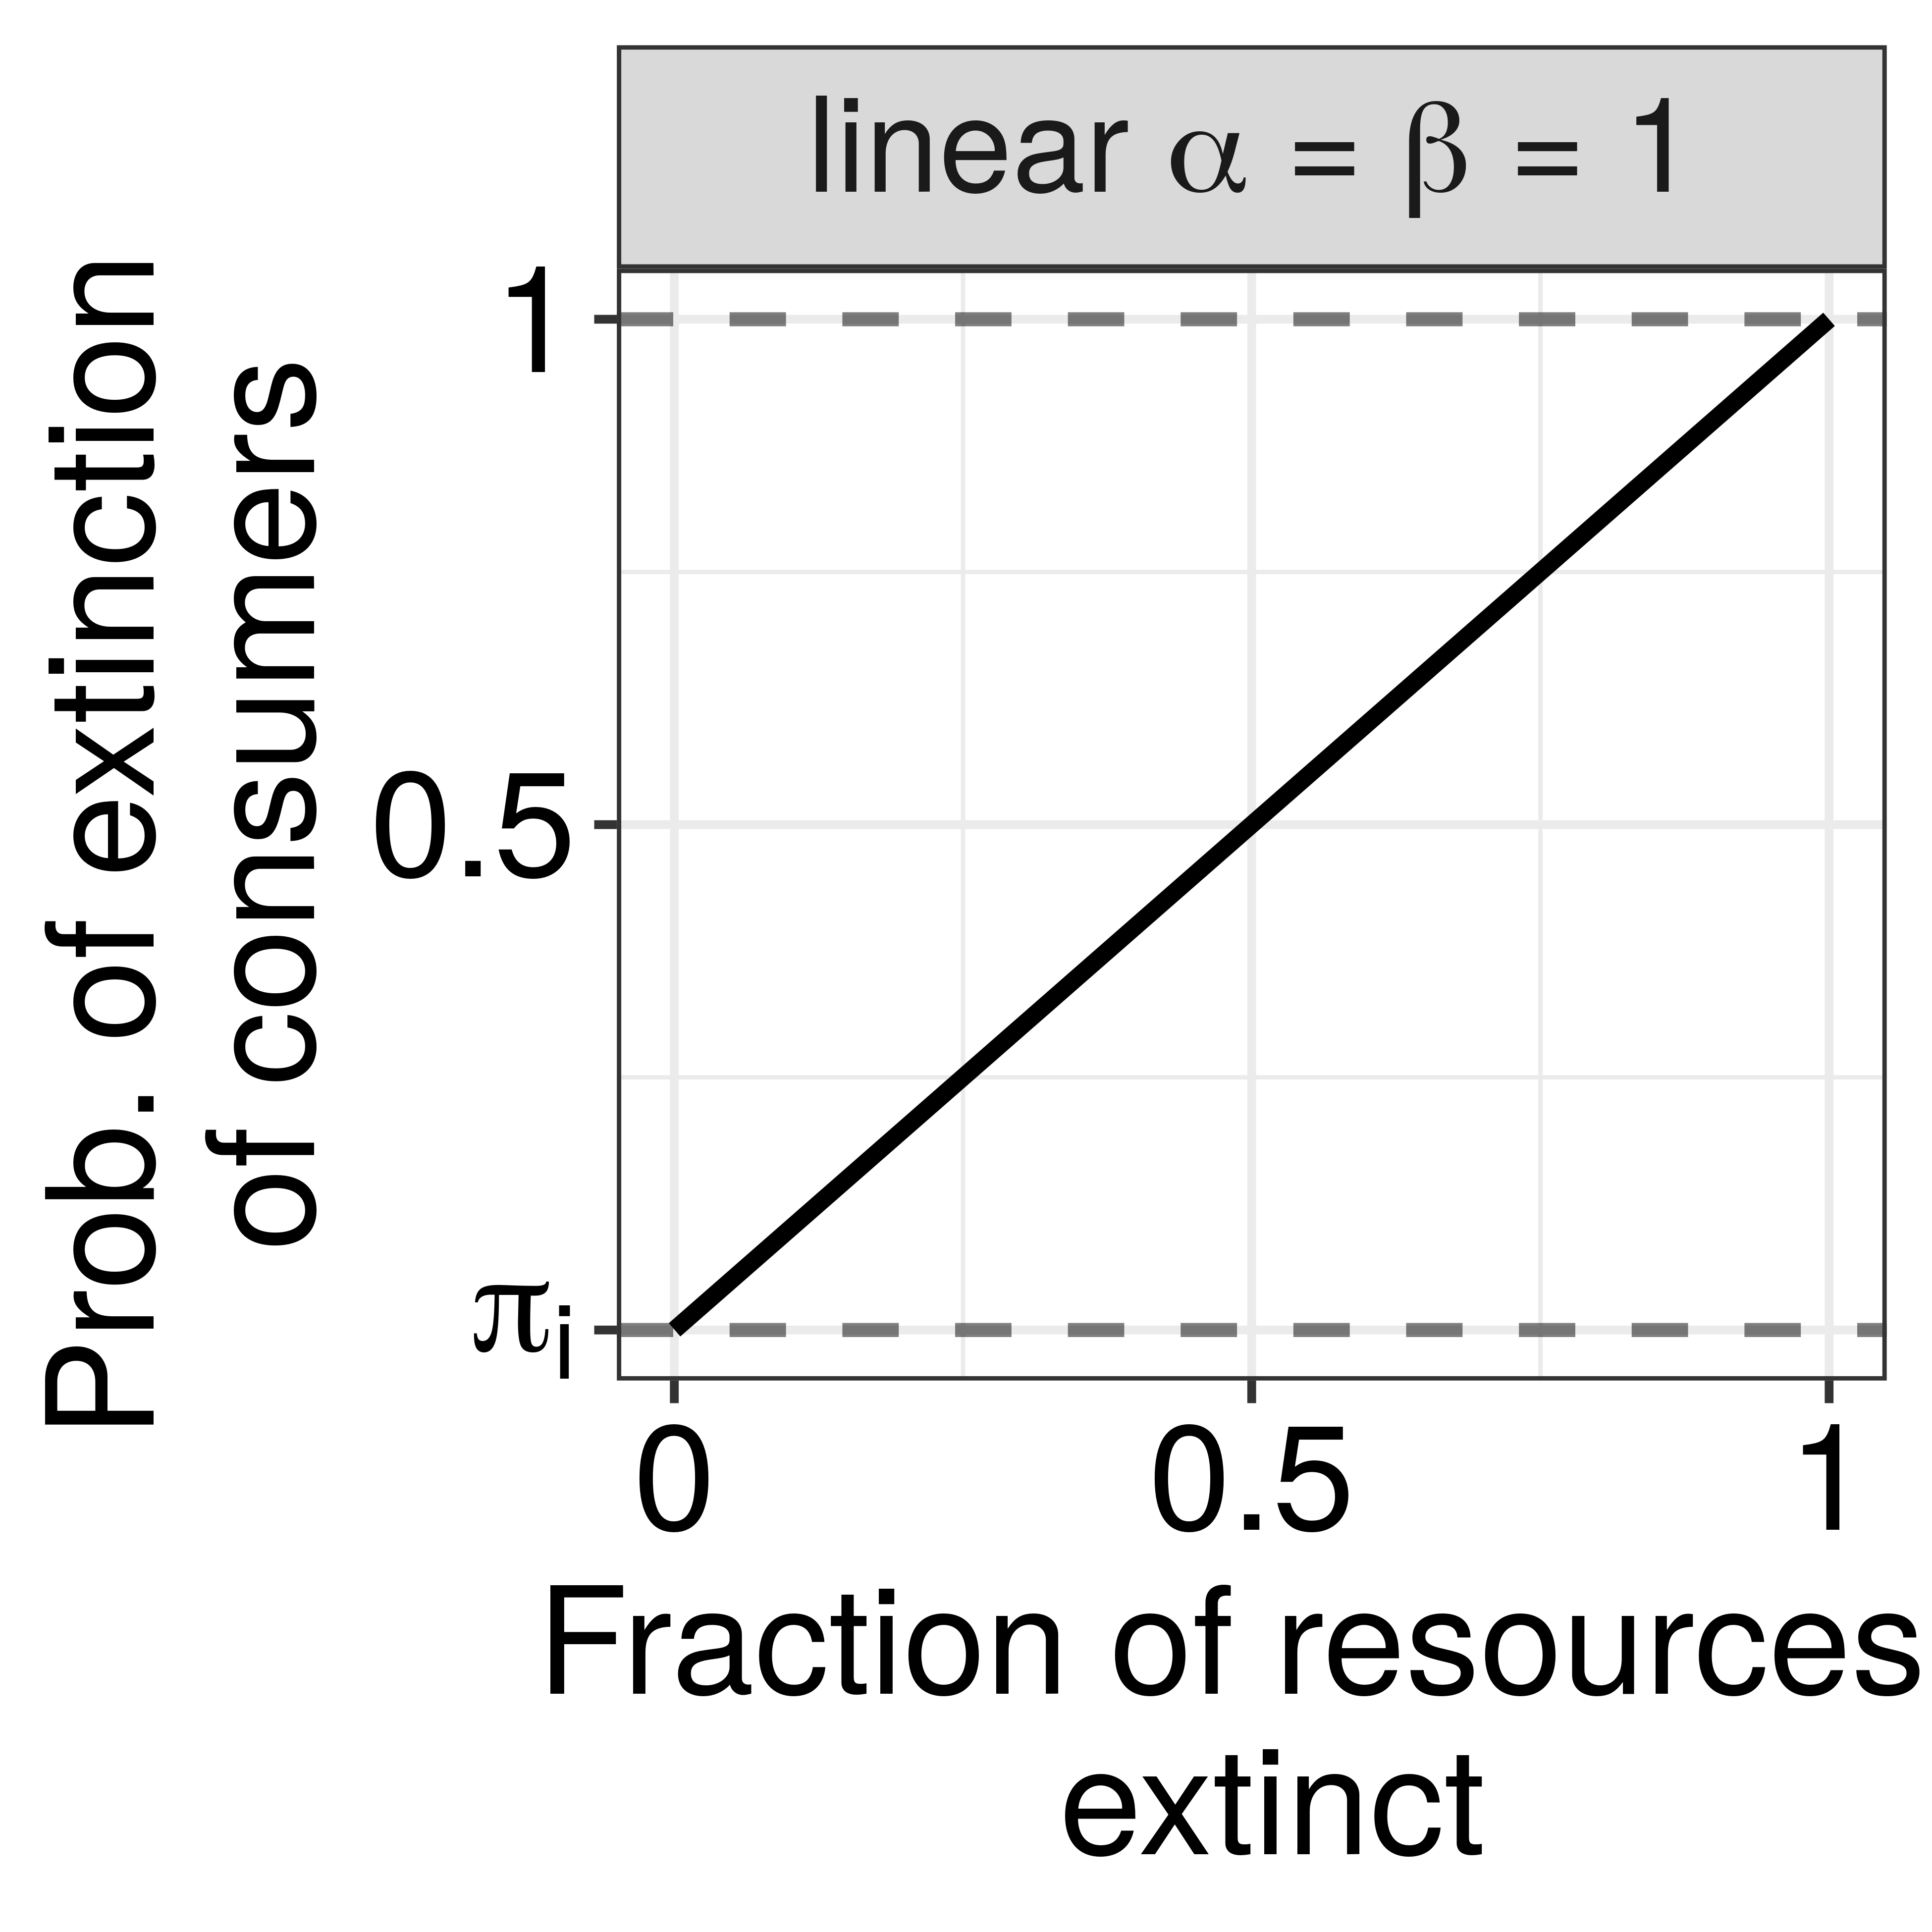
\includegraphics[width=0.19\textwidth,valign=t]{fform_1_1.png}
  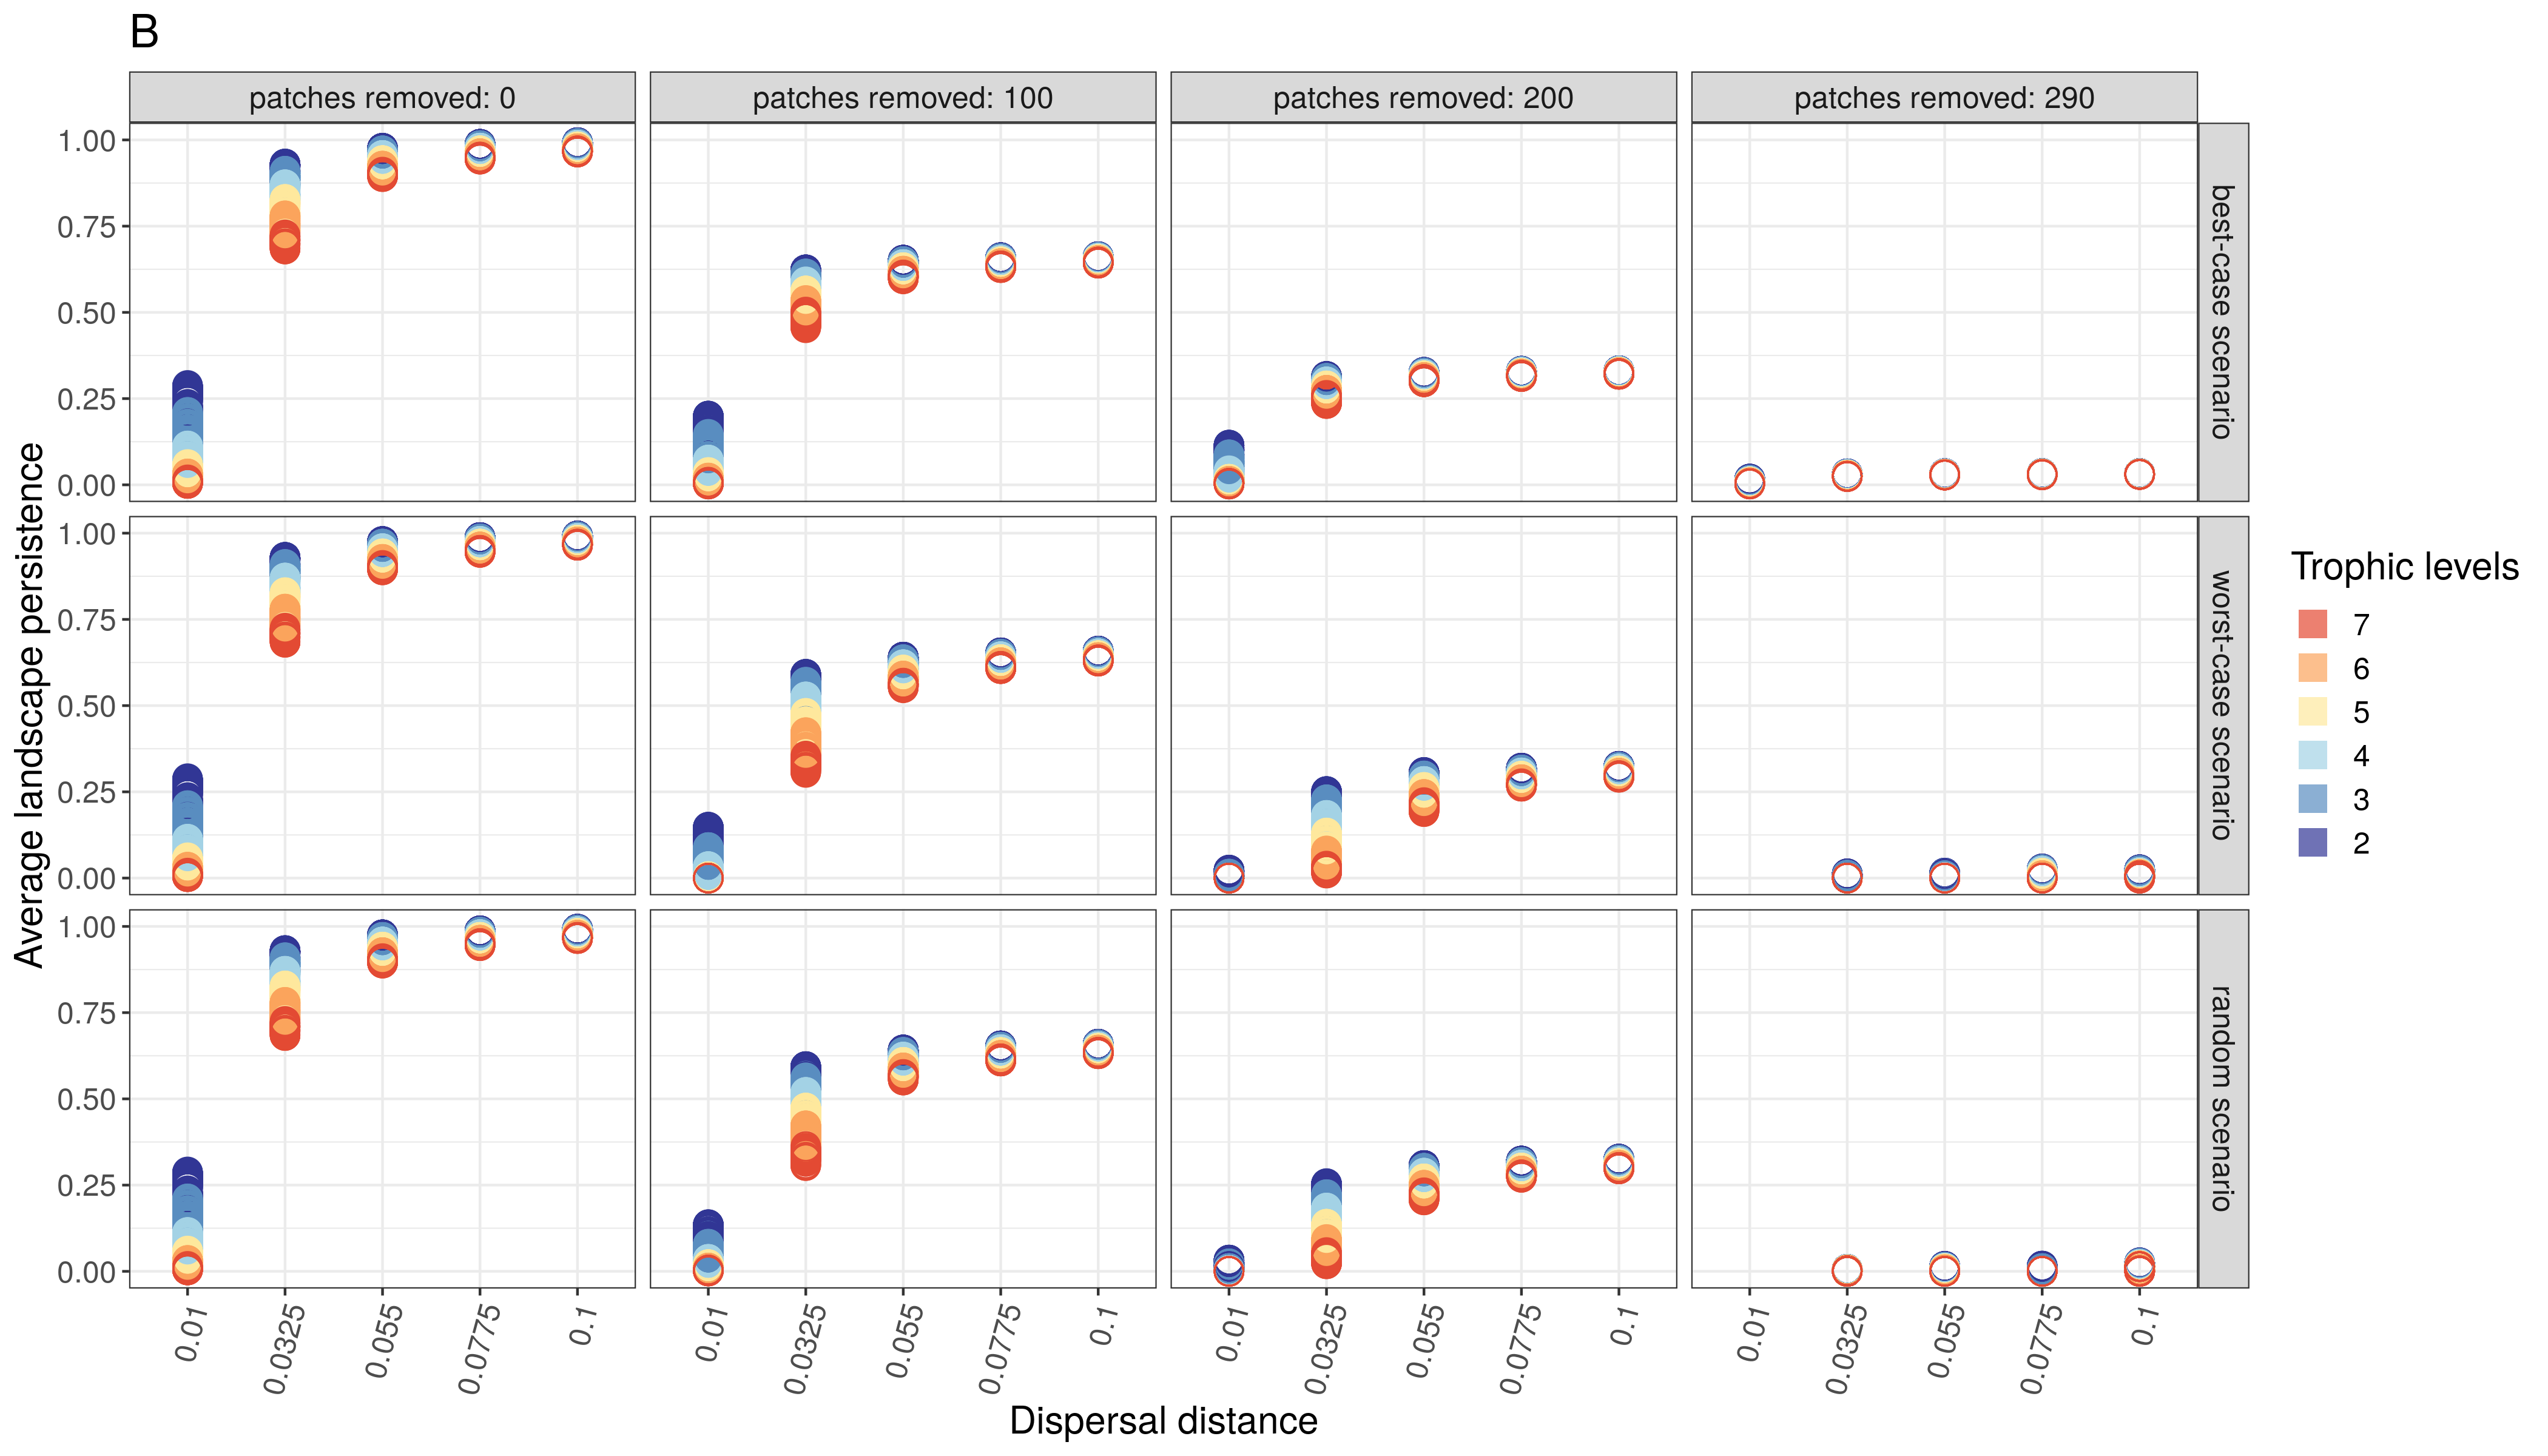
\includegraphics[width=0.8\textwidth,valign=t]{sump_Model_food_web_with_350_consumer_and_50_basal_species_basal_5_1.png}
    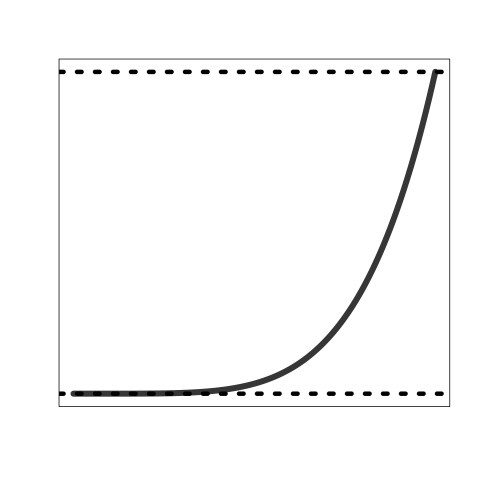
\includegraphics[width=0.19\textwidth,valign=t]{fform_5_1.png}
 \caption{As Figure \ref{S_fig:patchloss_300_100_distance_1}, but with 350 consumer and 50 basal species.}
\end{figure}

\begin{figure}[!ht]\ContinuedFloat
  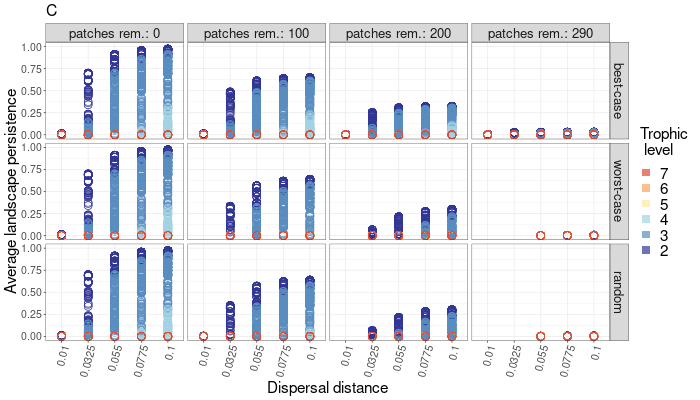
\includegraphics[width=0.8\textwidth,valign=t]{sump_Model_food_web_with_350_consumer_and_50_basal_species_basal_1_5.png}
  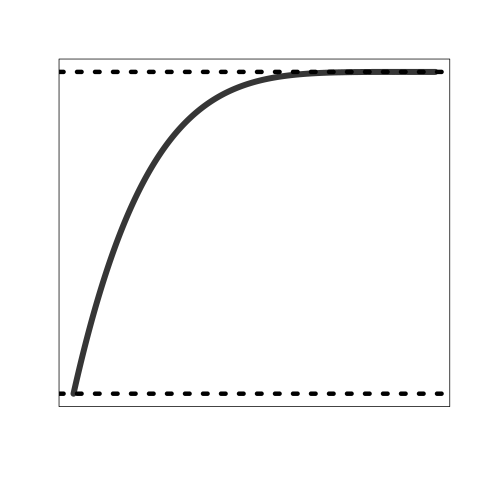
\includegraphics[width=0.19\textwidth,valign=t]{fform_1_5.png}
  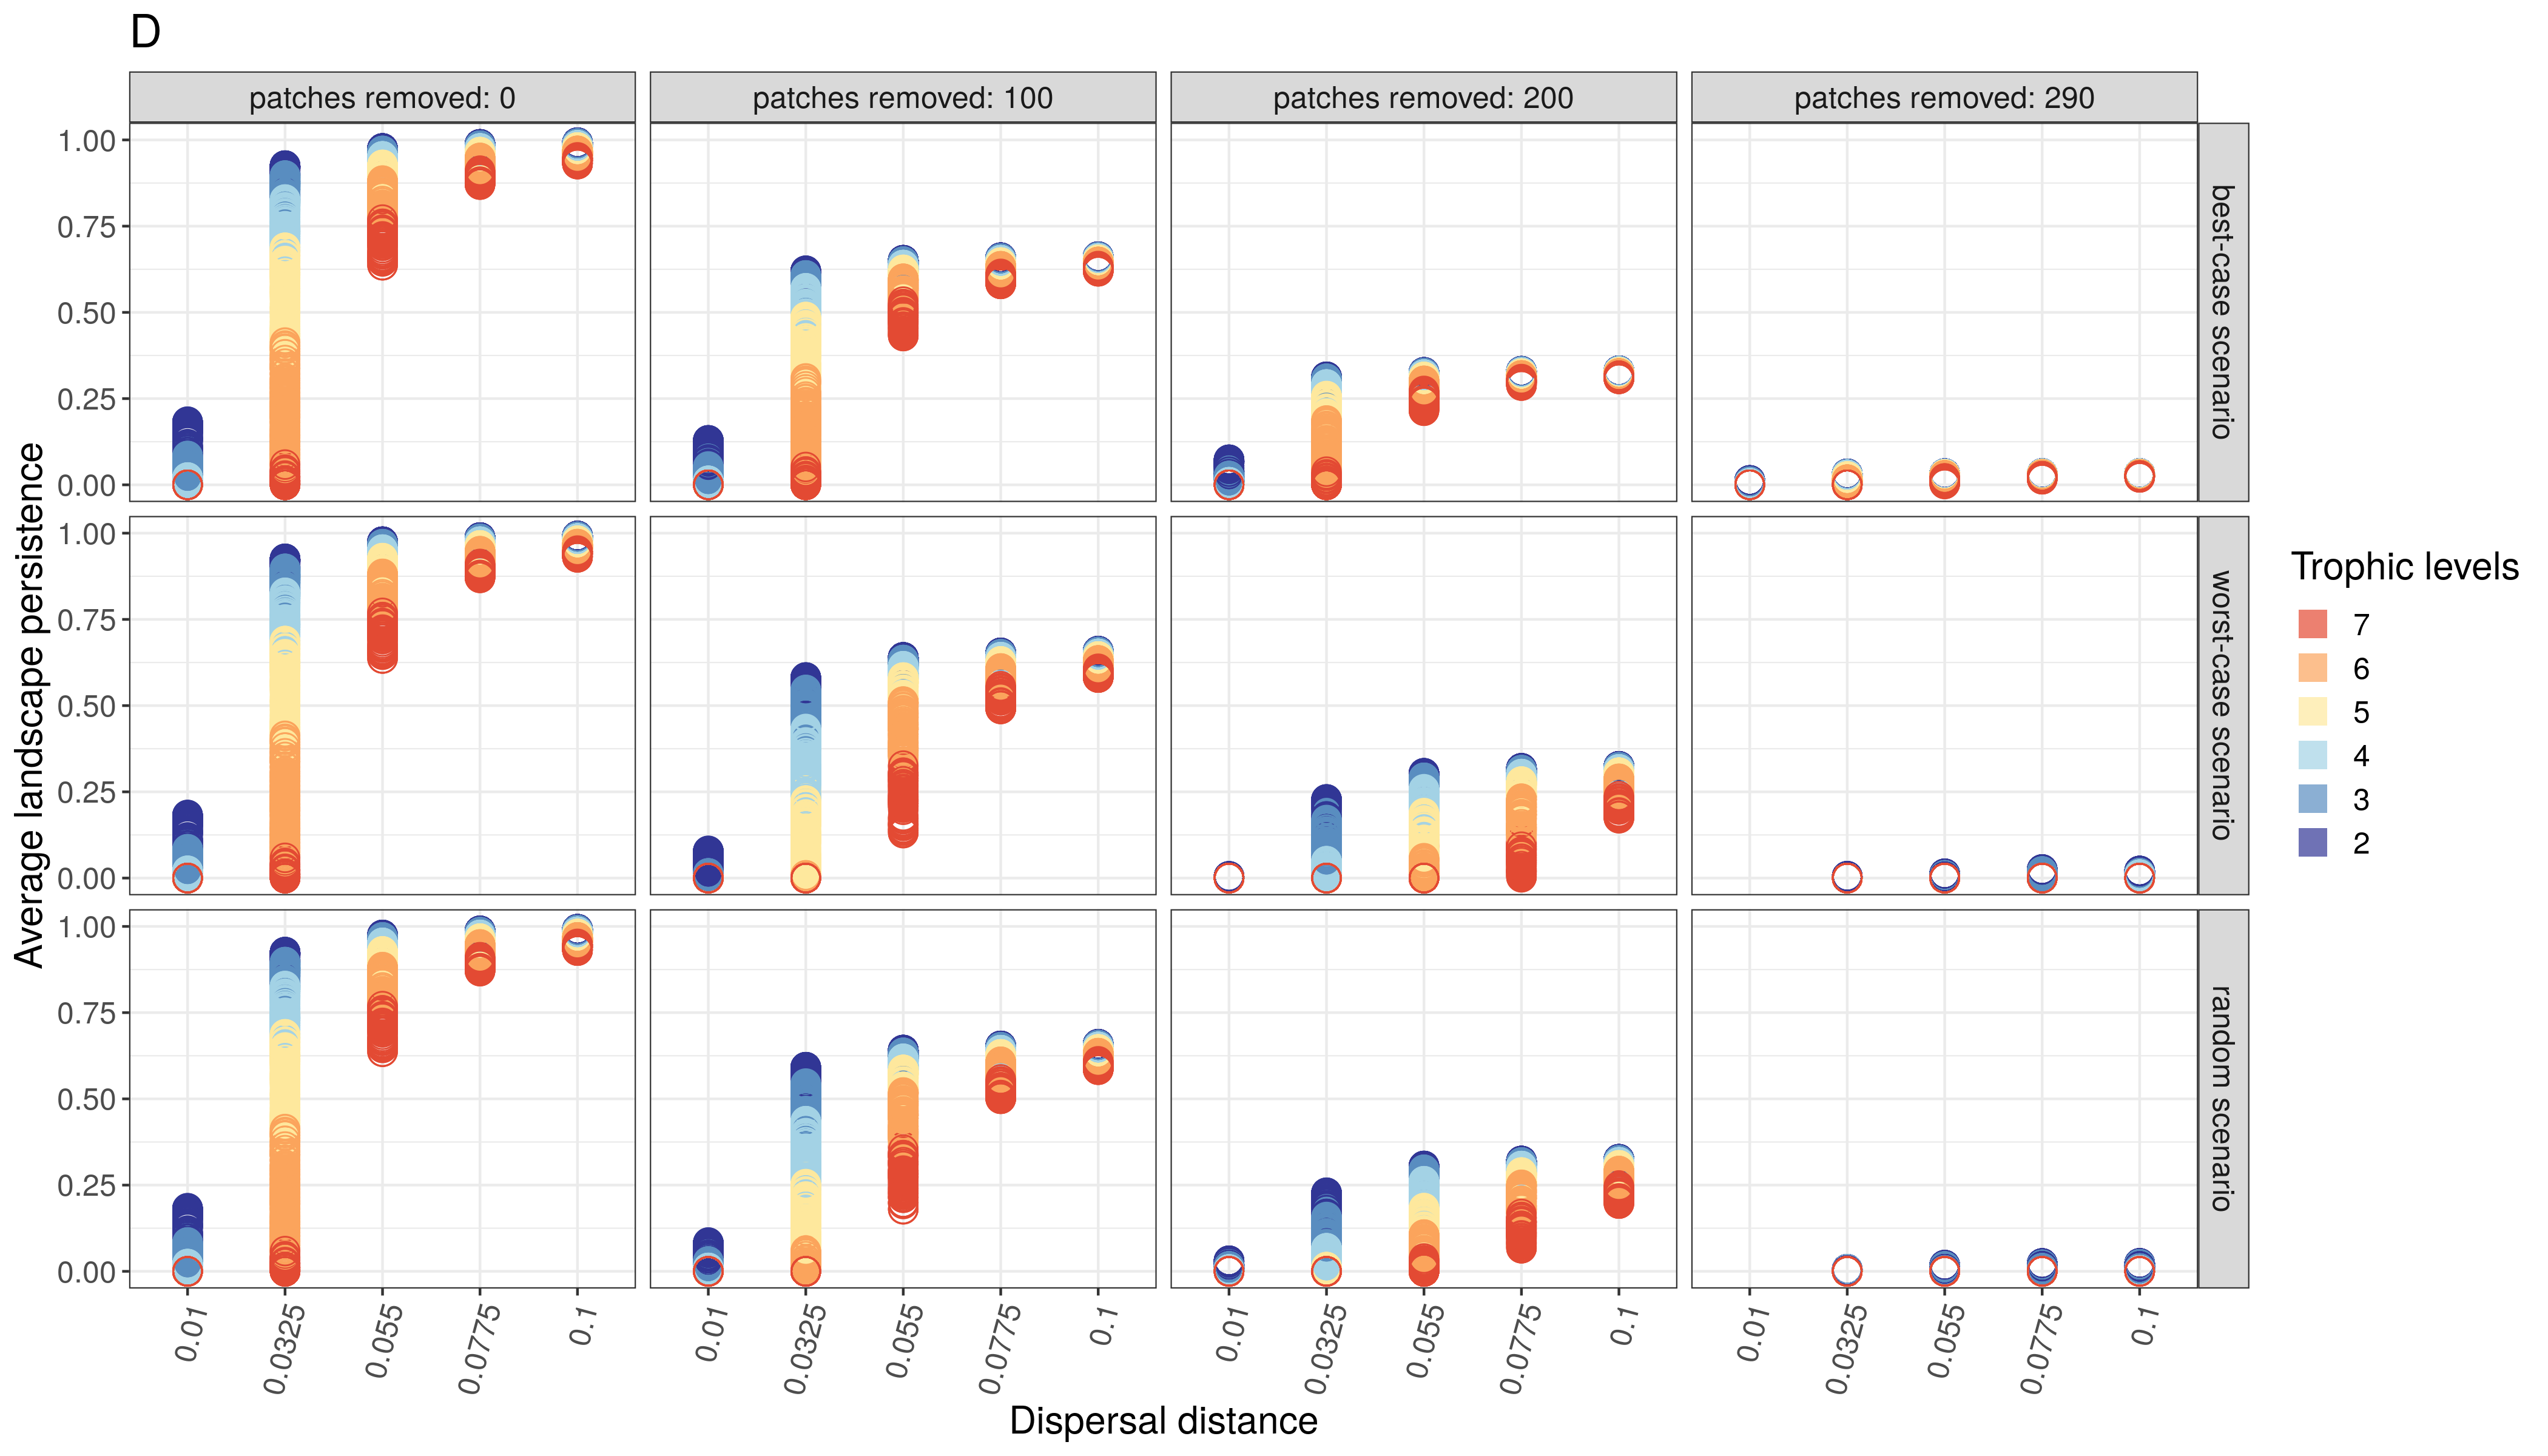
\includegraphics[width=0.8\textwidth,valign=t]{sump_Model_food_web_with_350_consumer_and_50_basal_species_basal_5_5.png}
  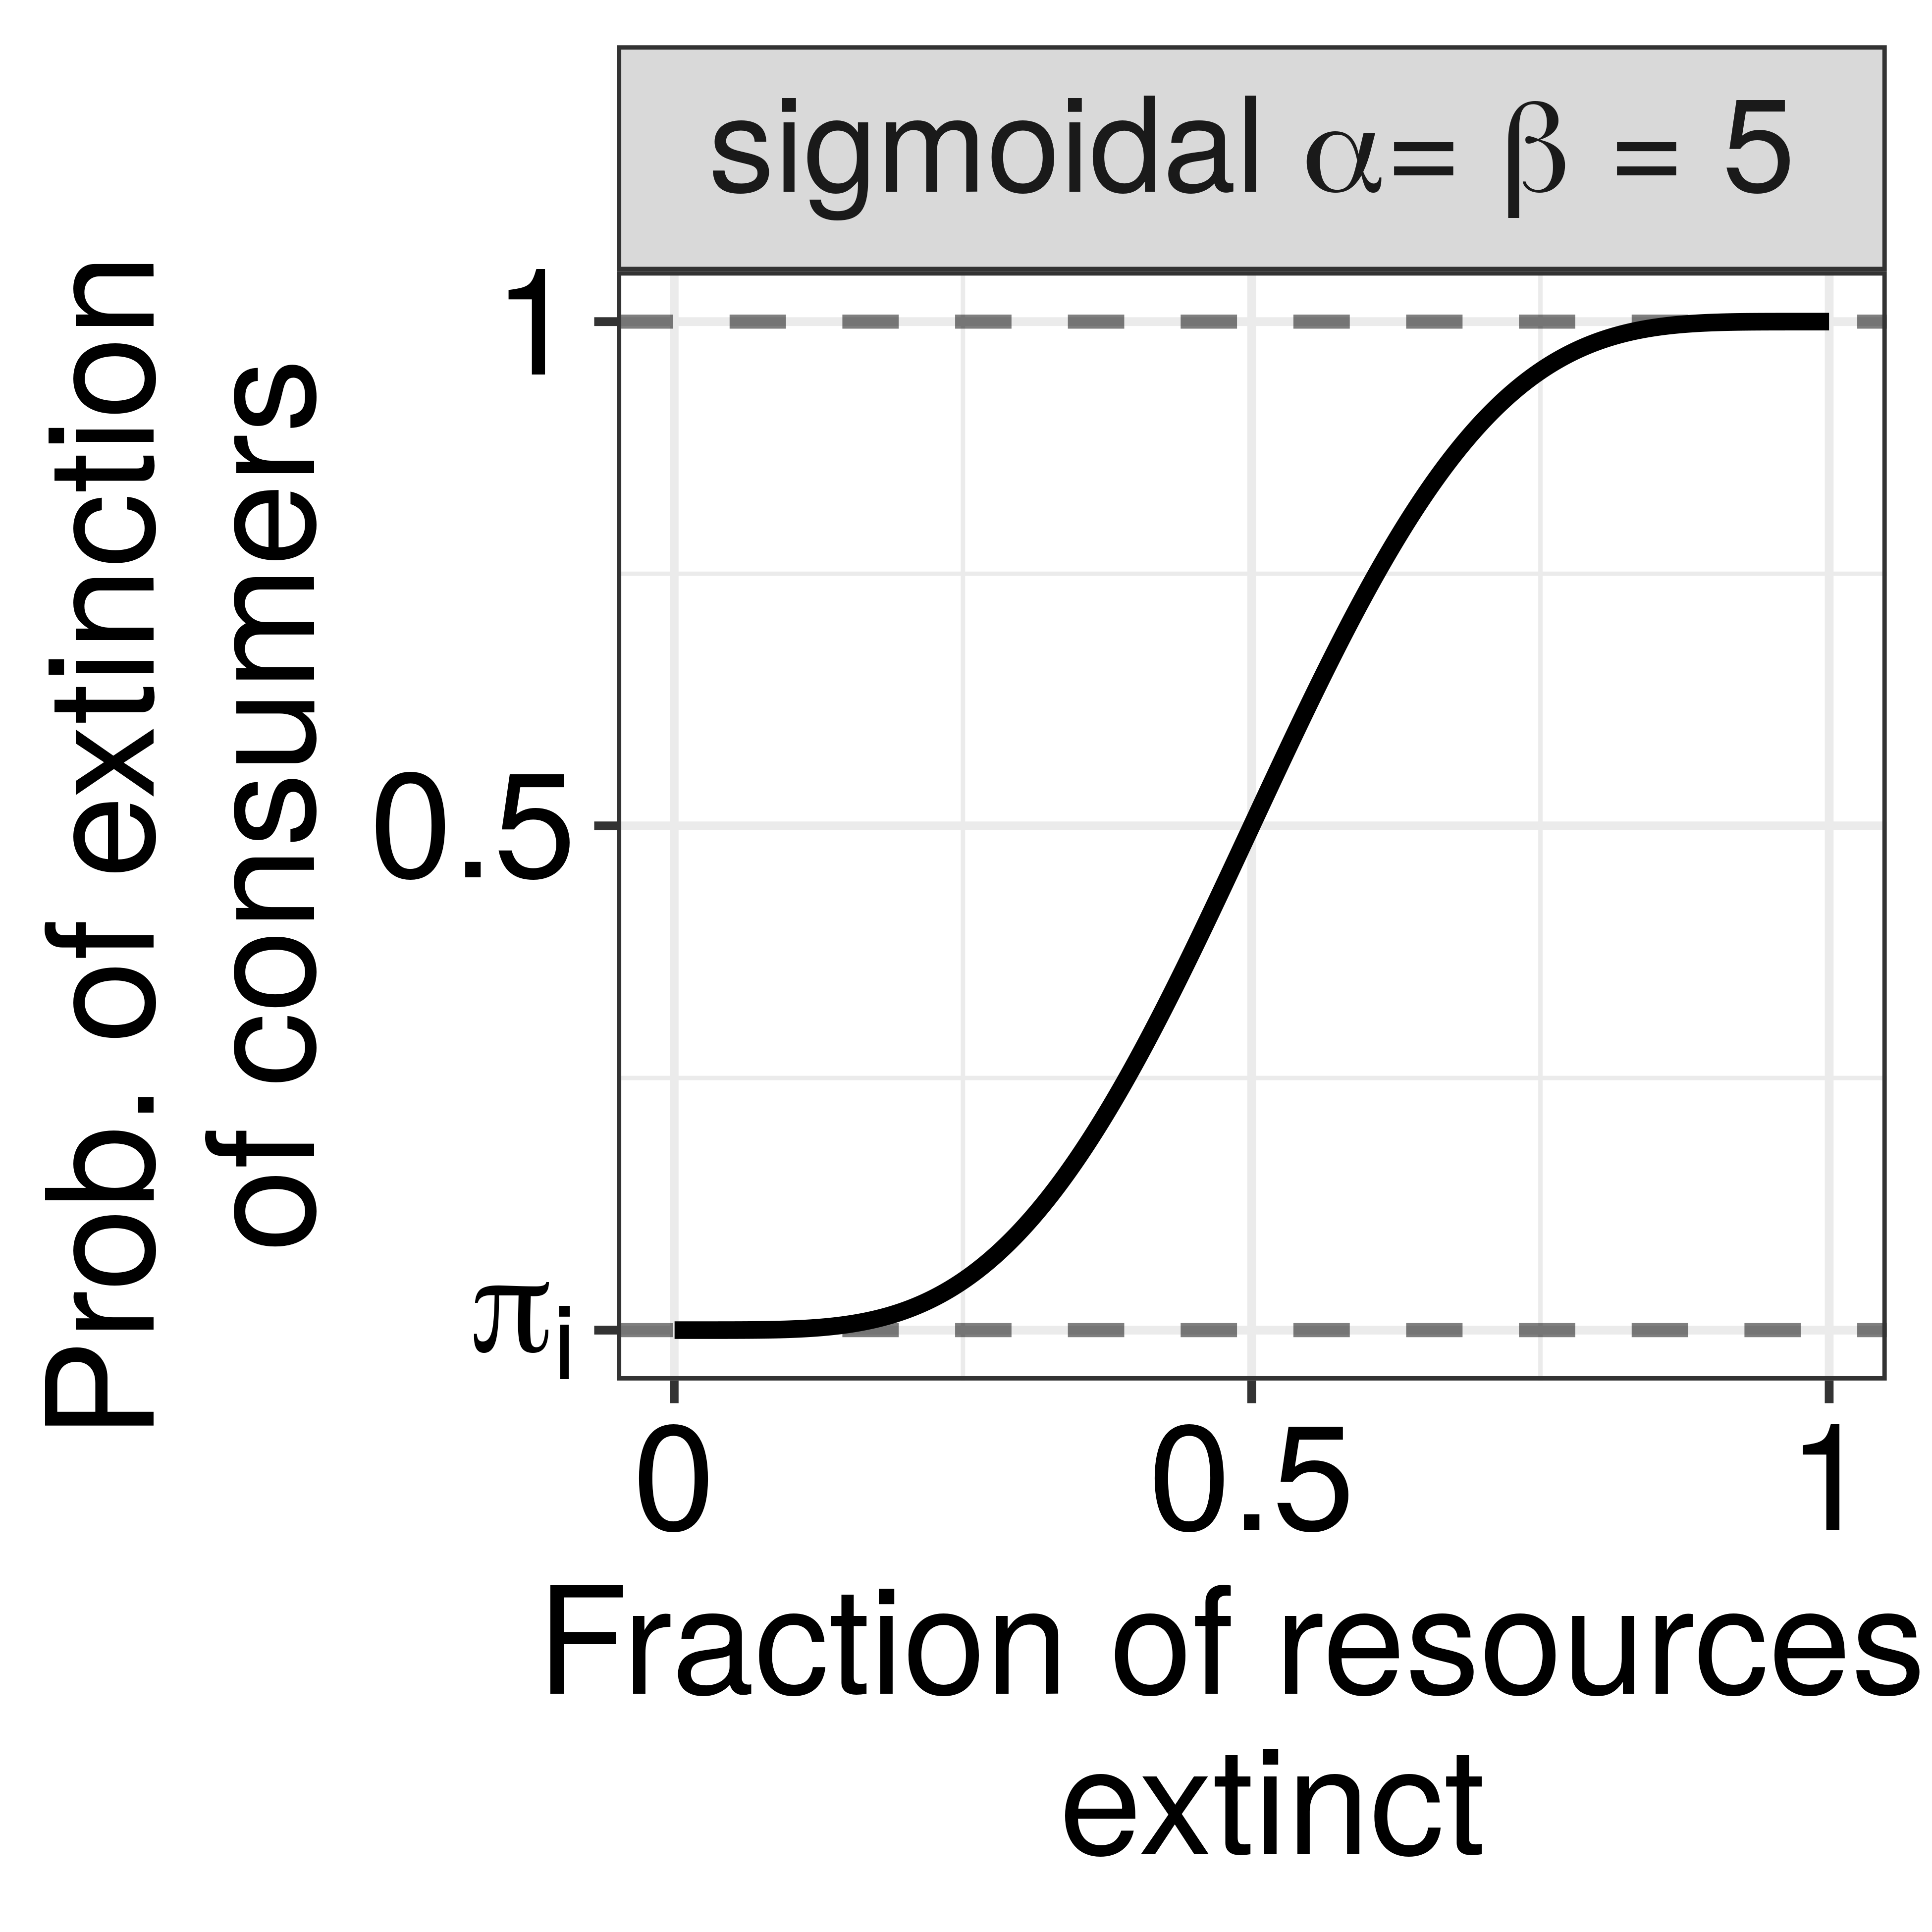
\includegraphics[width=0.19\textwidth,valign=t]{fform_5_5.png}
 \caption{Figure continued.}
 \label{S_fig:patchloss_350_50_distance_2}
\end{figure}

\begin{figure}[!ht]
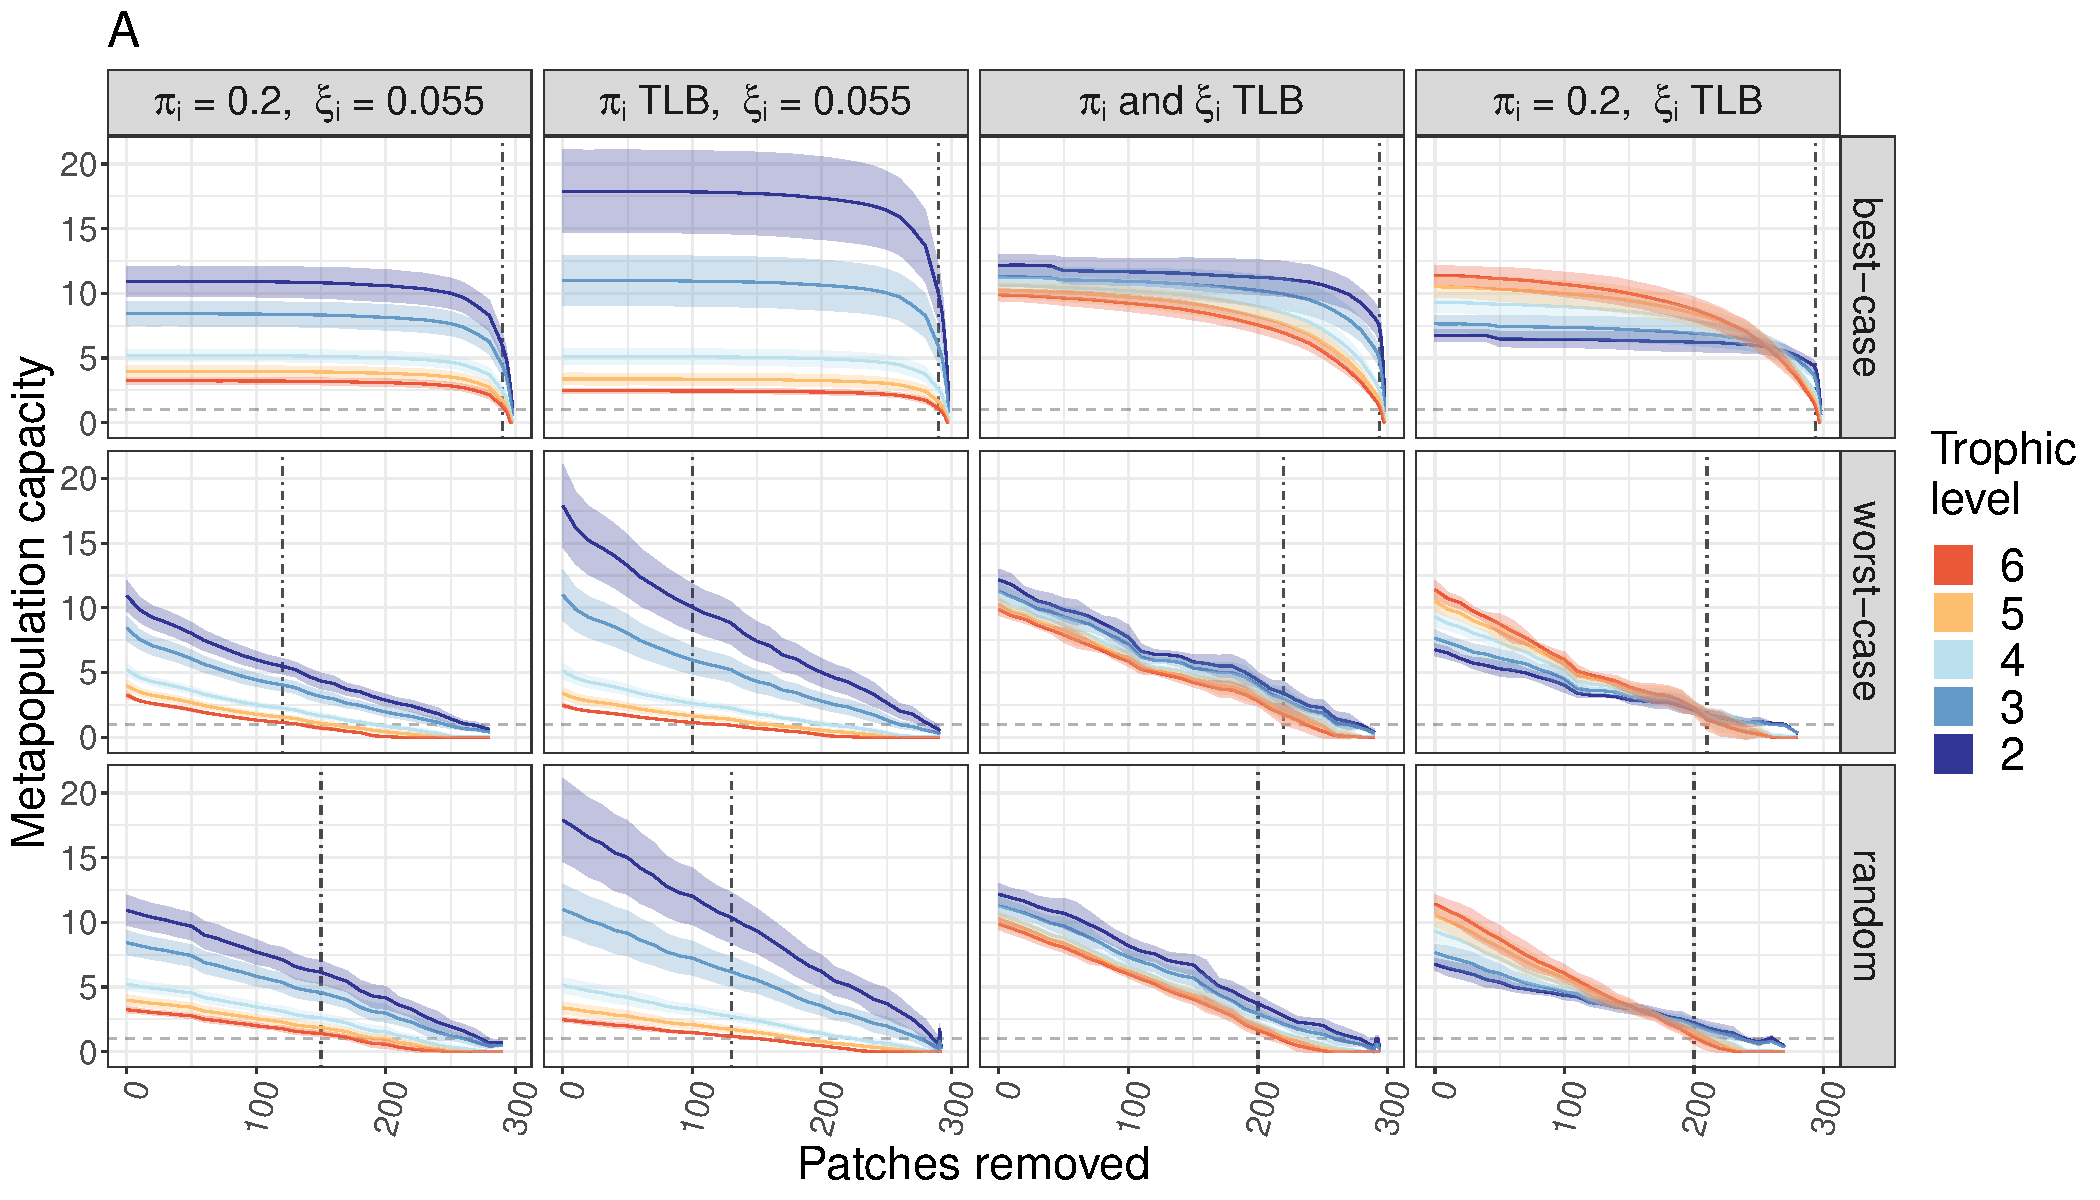
\includegraphics[width=0.8\textwidth,valign=t]{lambda_Model_food_web_with_250_consumer_and_150_basal_species_basal_1_1.pdf}
  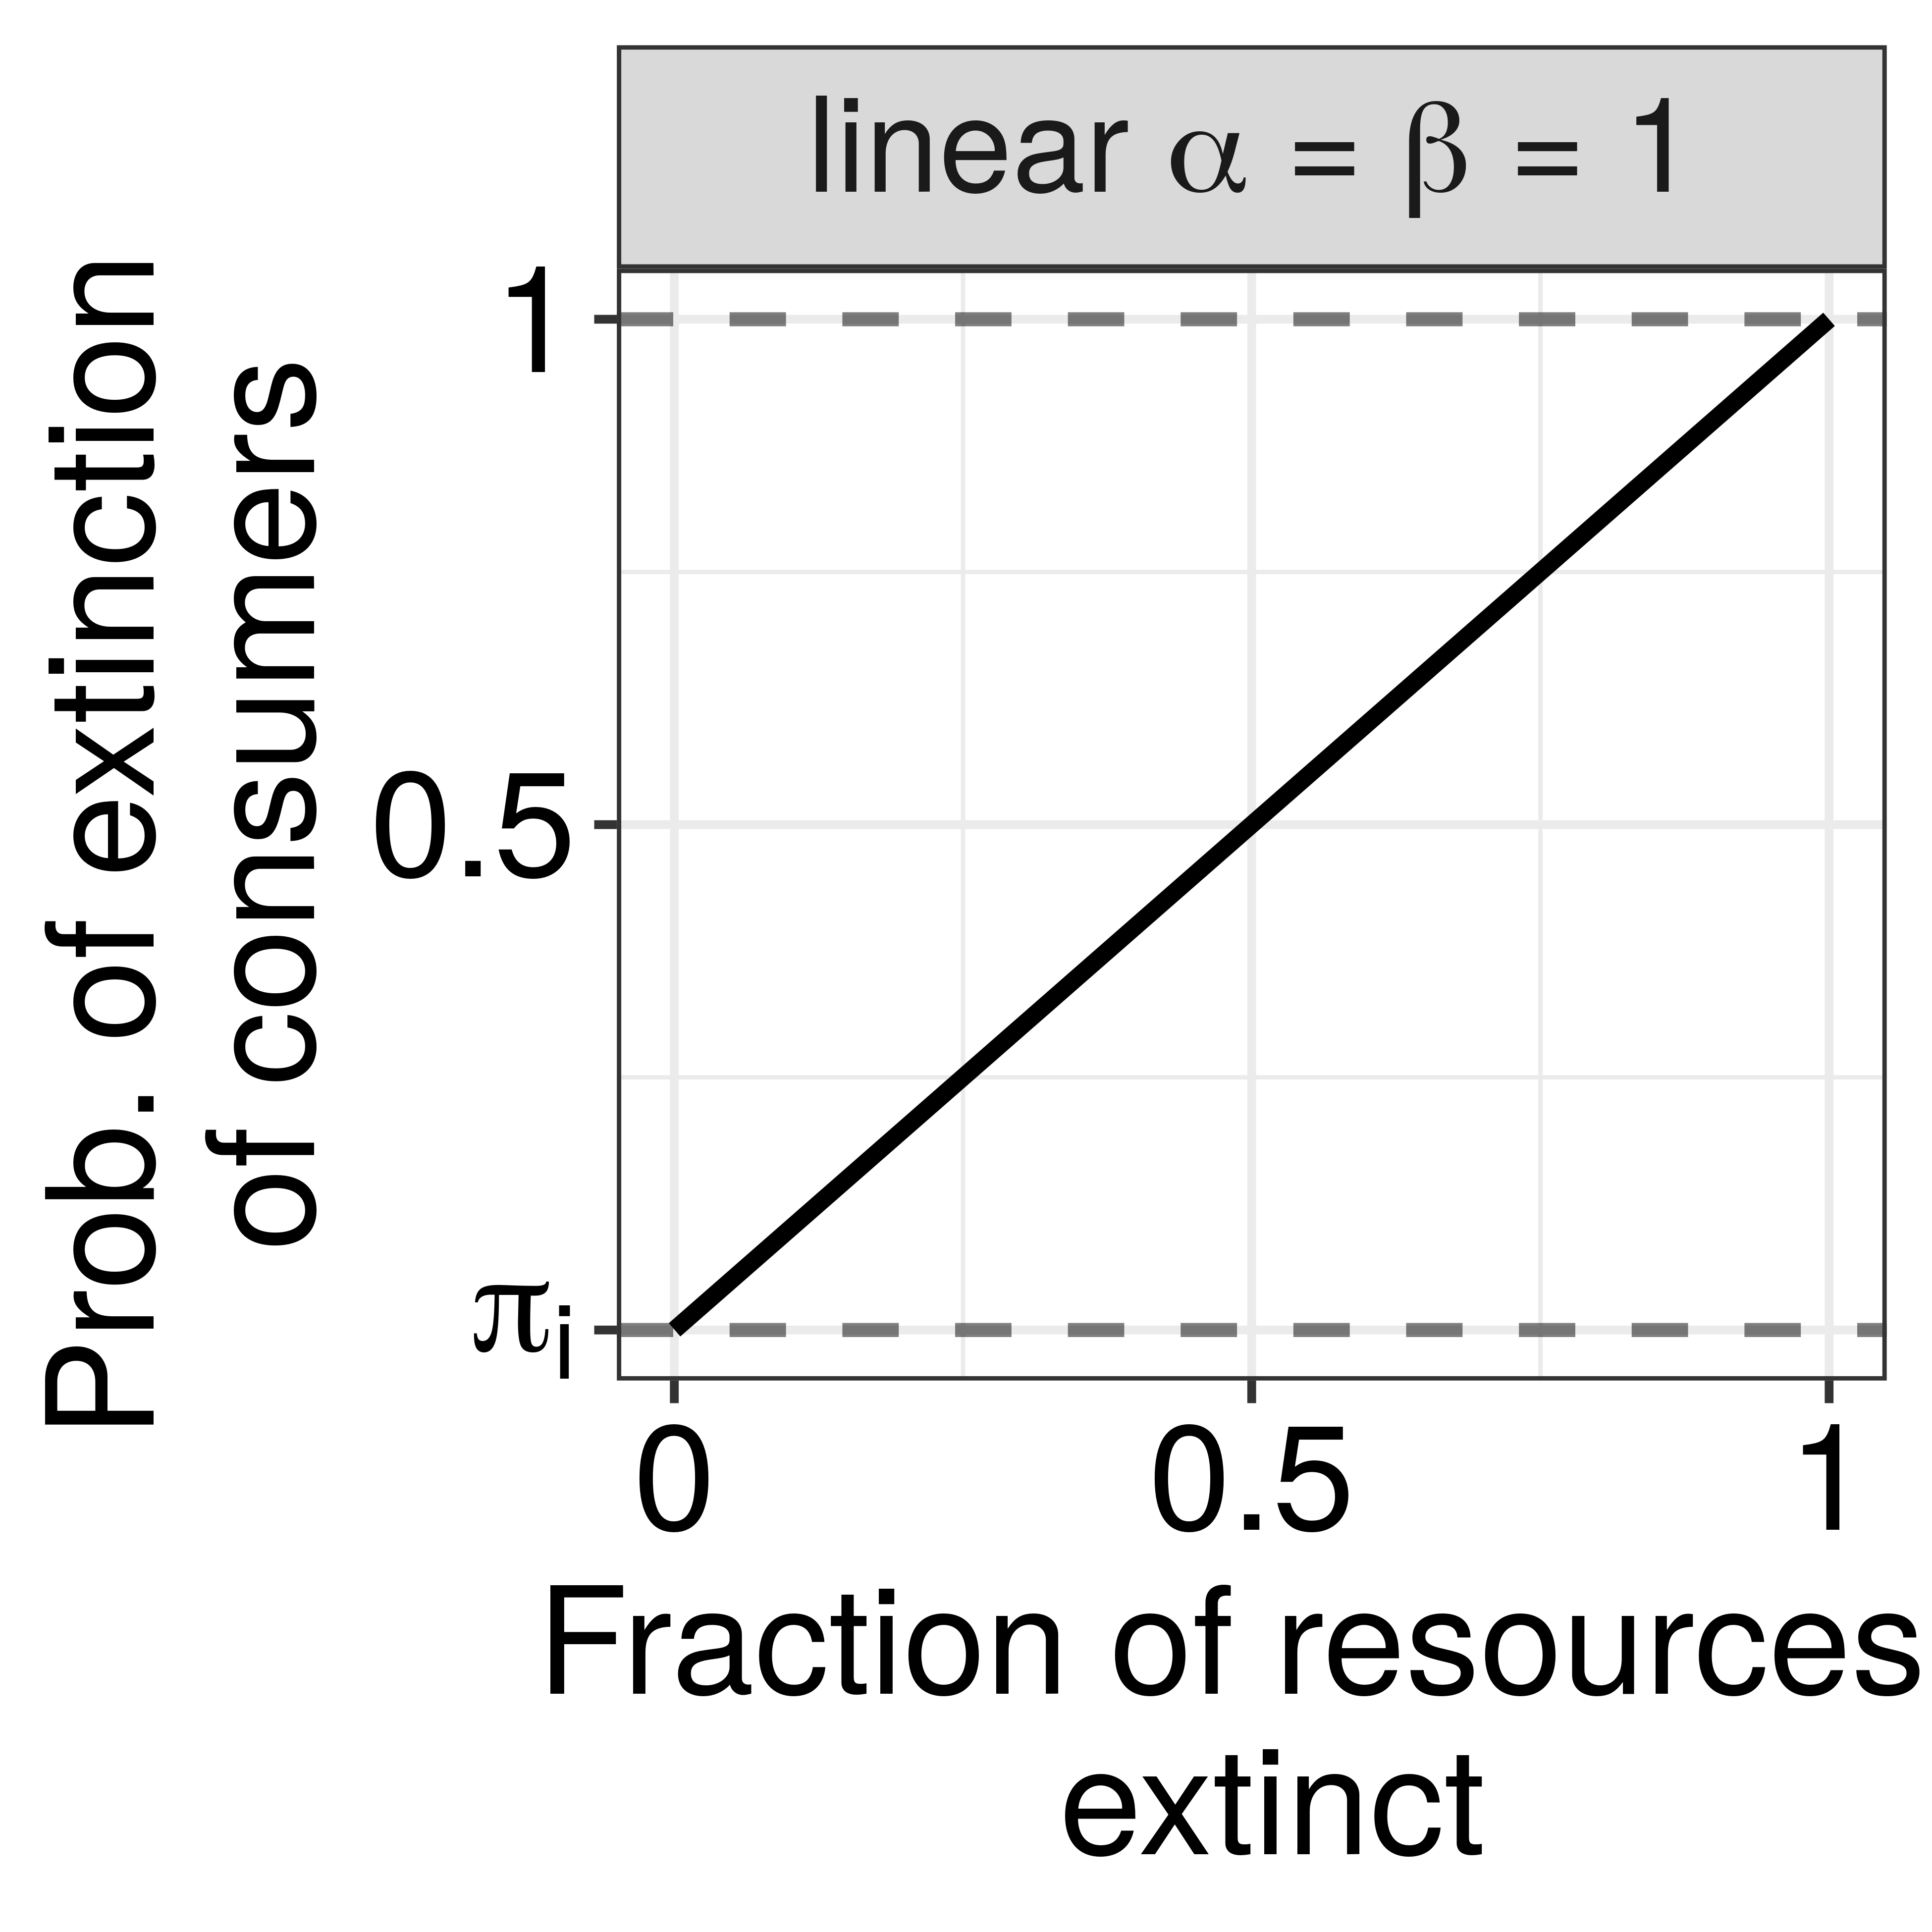
\includegraphics[width=0.19\textwidth,valign=t]{fform_1_1.png}
  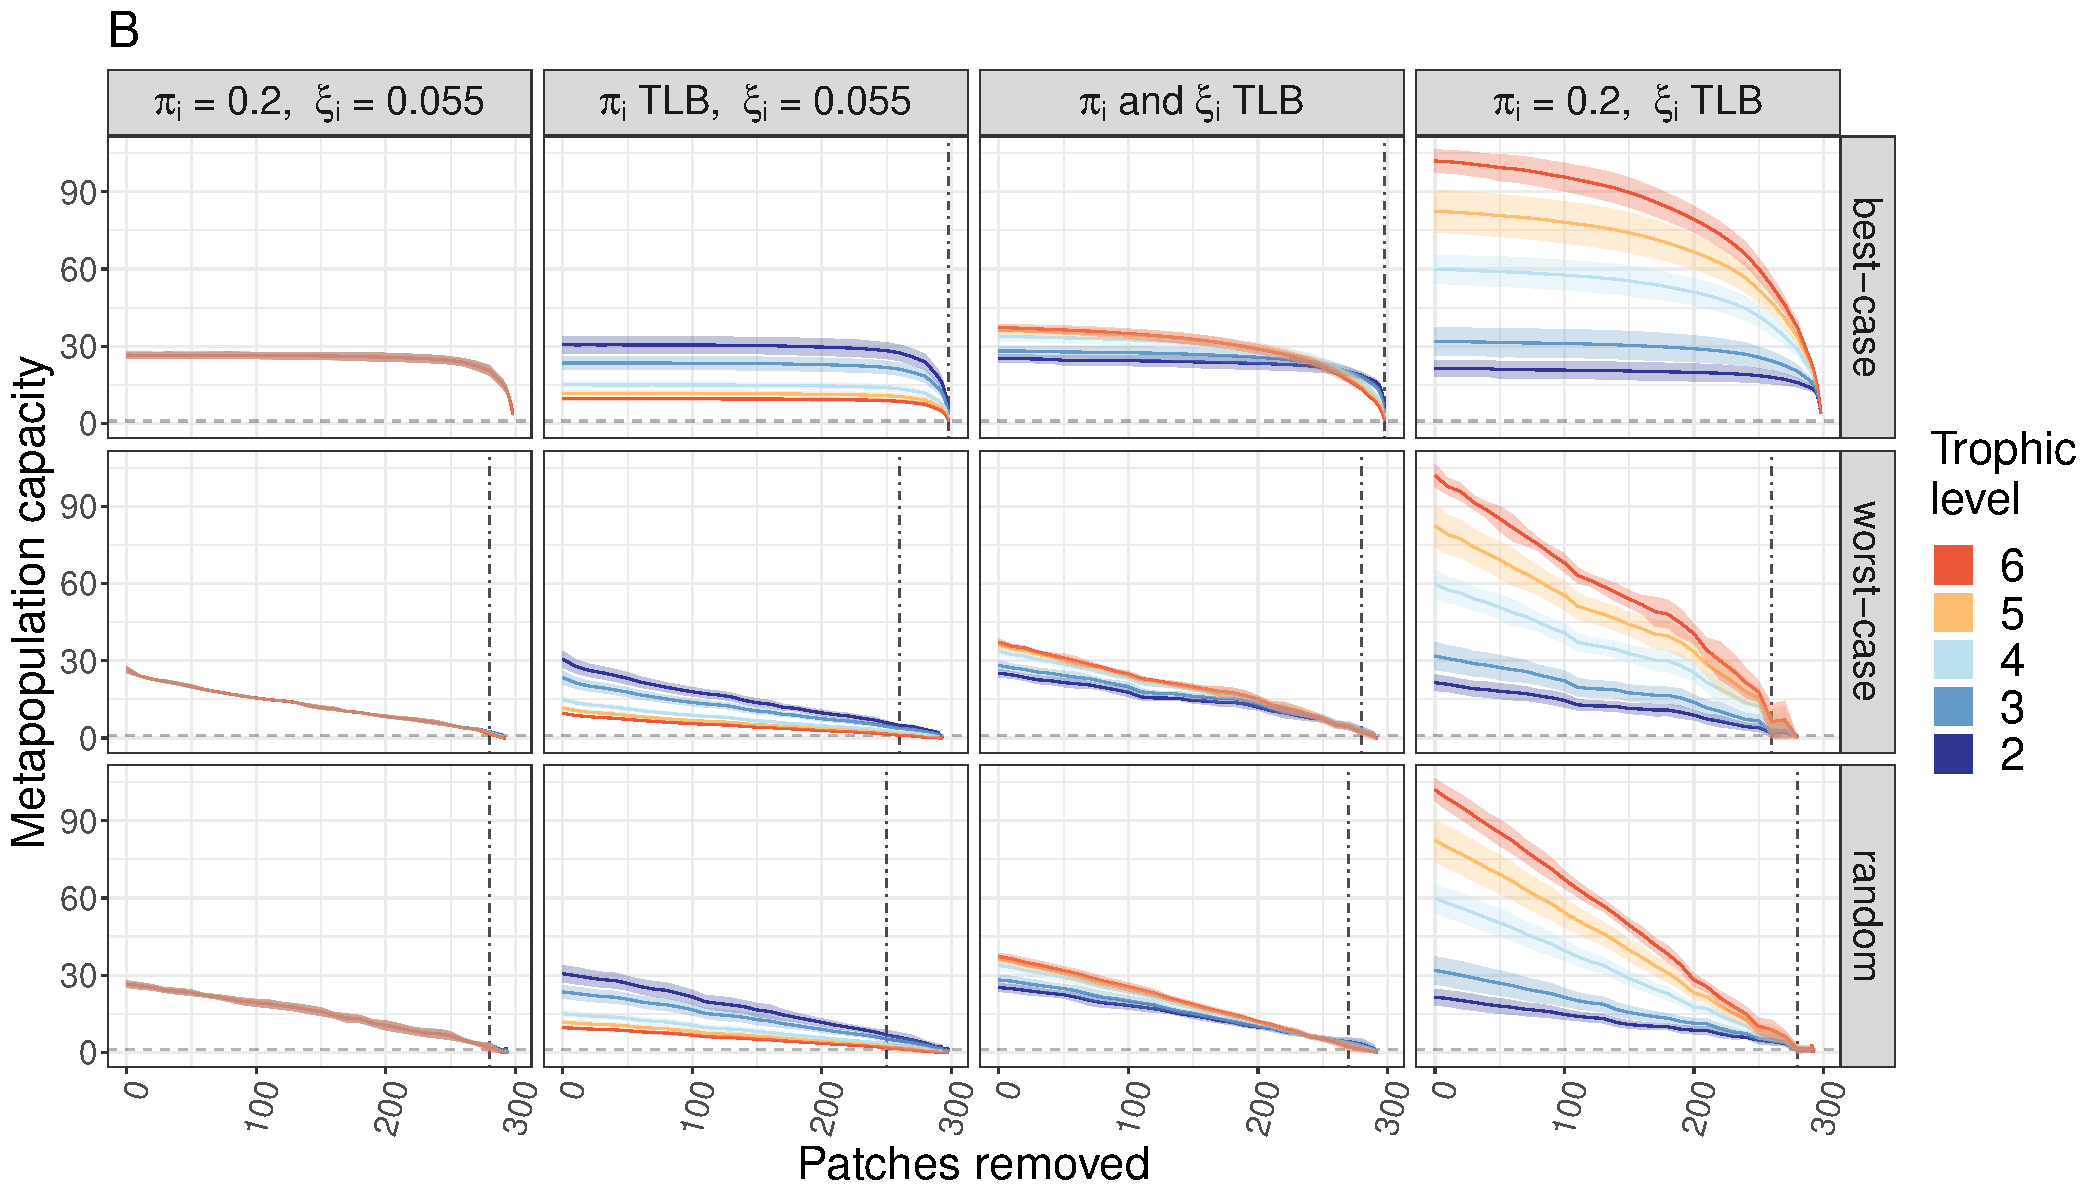
\includegraphics[width=0.8\textwidth,valign=t]{lambda_Model_food_web_with_250_consumer_and_150_basal_species_basal_5_1.pdf}
    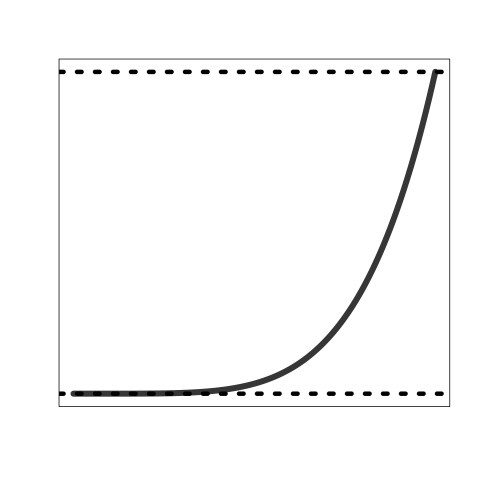
\includegraphics[width=0.19\textwidth,valign=t]{fform_5_1.png}
 \caption{As Figure \ref{S_fig:patchloss_350_50_1}, but with 250 consumer and 150 basal species.} 
\end{figure}

\begin{figure}\ContinuedFloat
 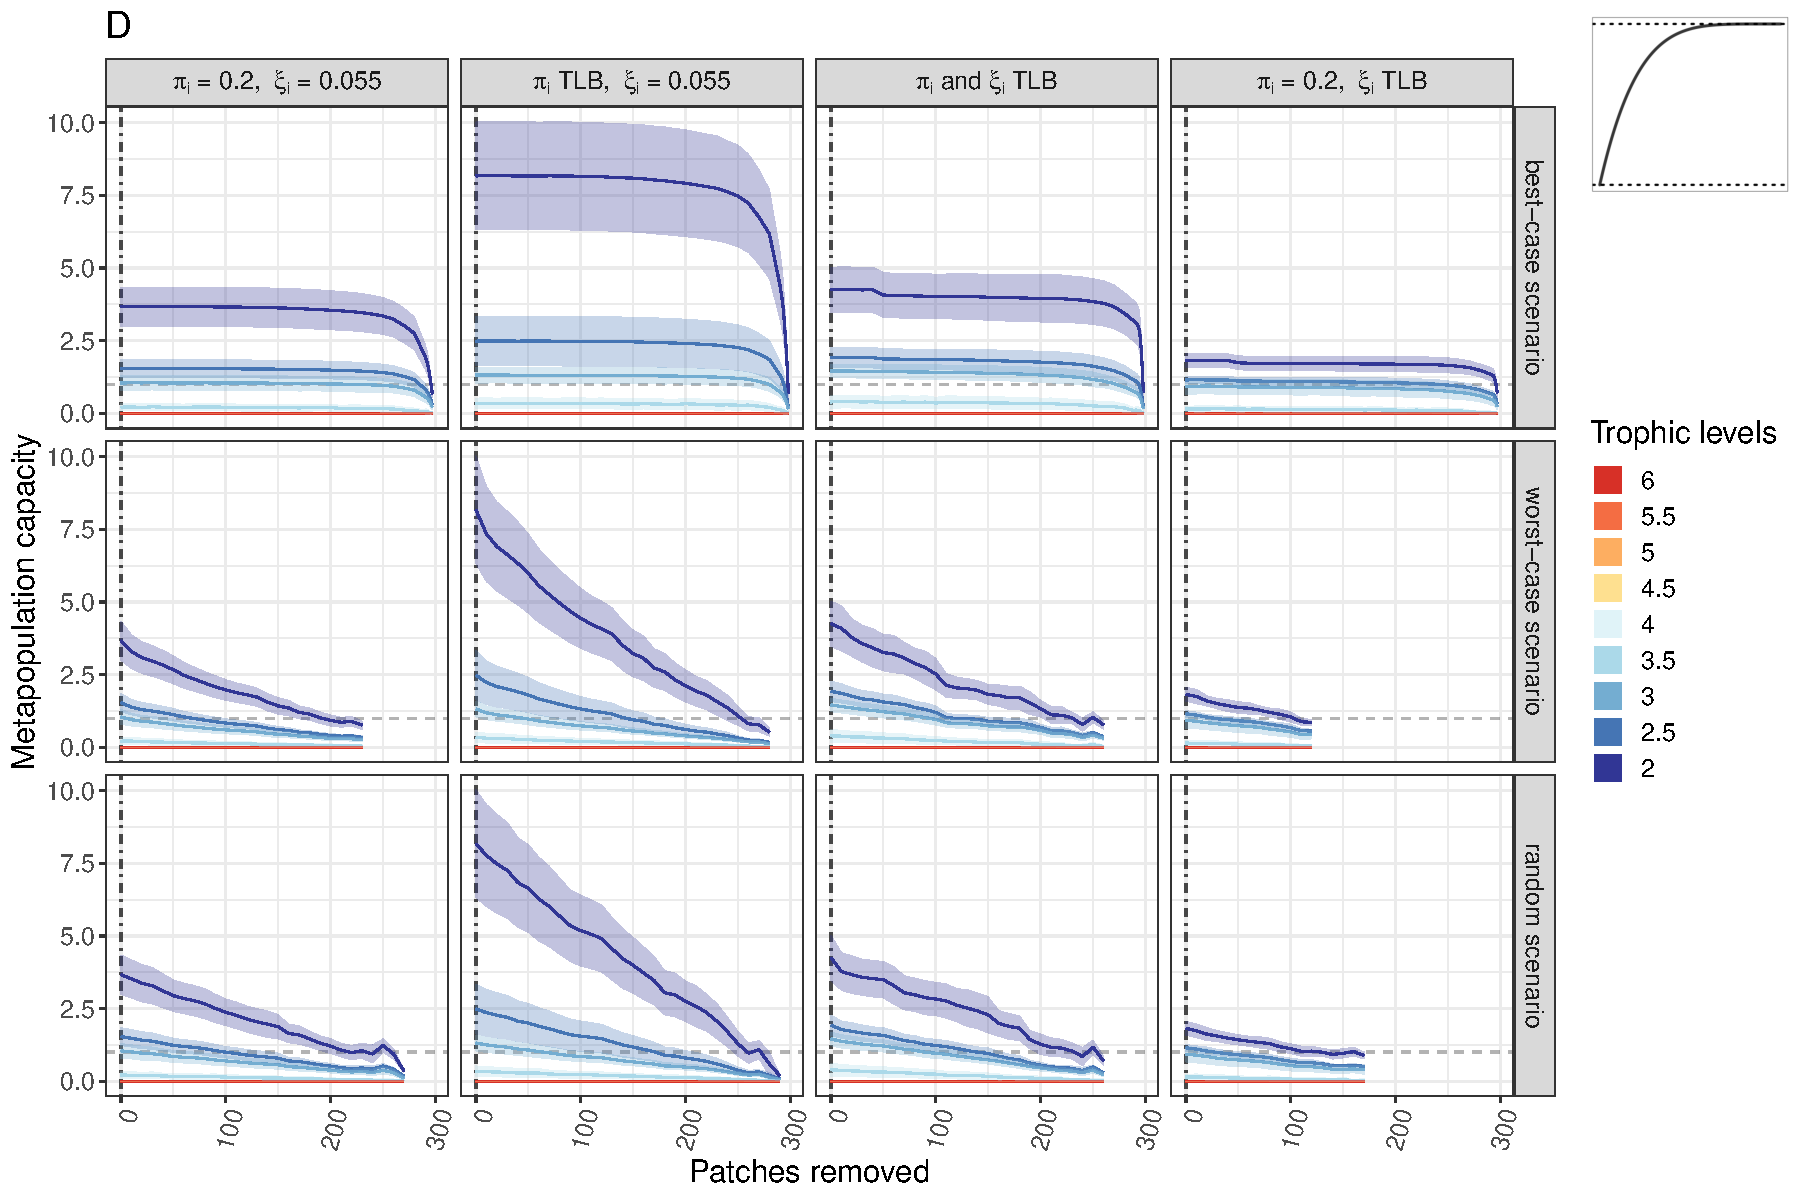
\includegraphics[width=0.8\textwidth,valign=t]{lambda_Model_food_web_with_250_consumer_and_150_basal_species_basal_1_5.pdf}
  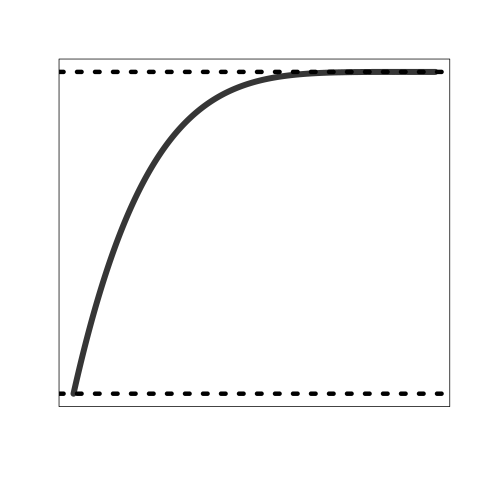
\includegraphics[width=0.19\textwidth,valign=t]{fform_1_5.png}
  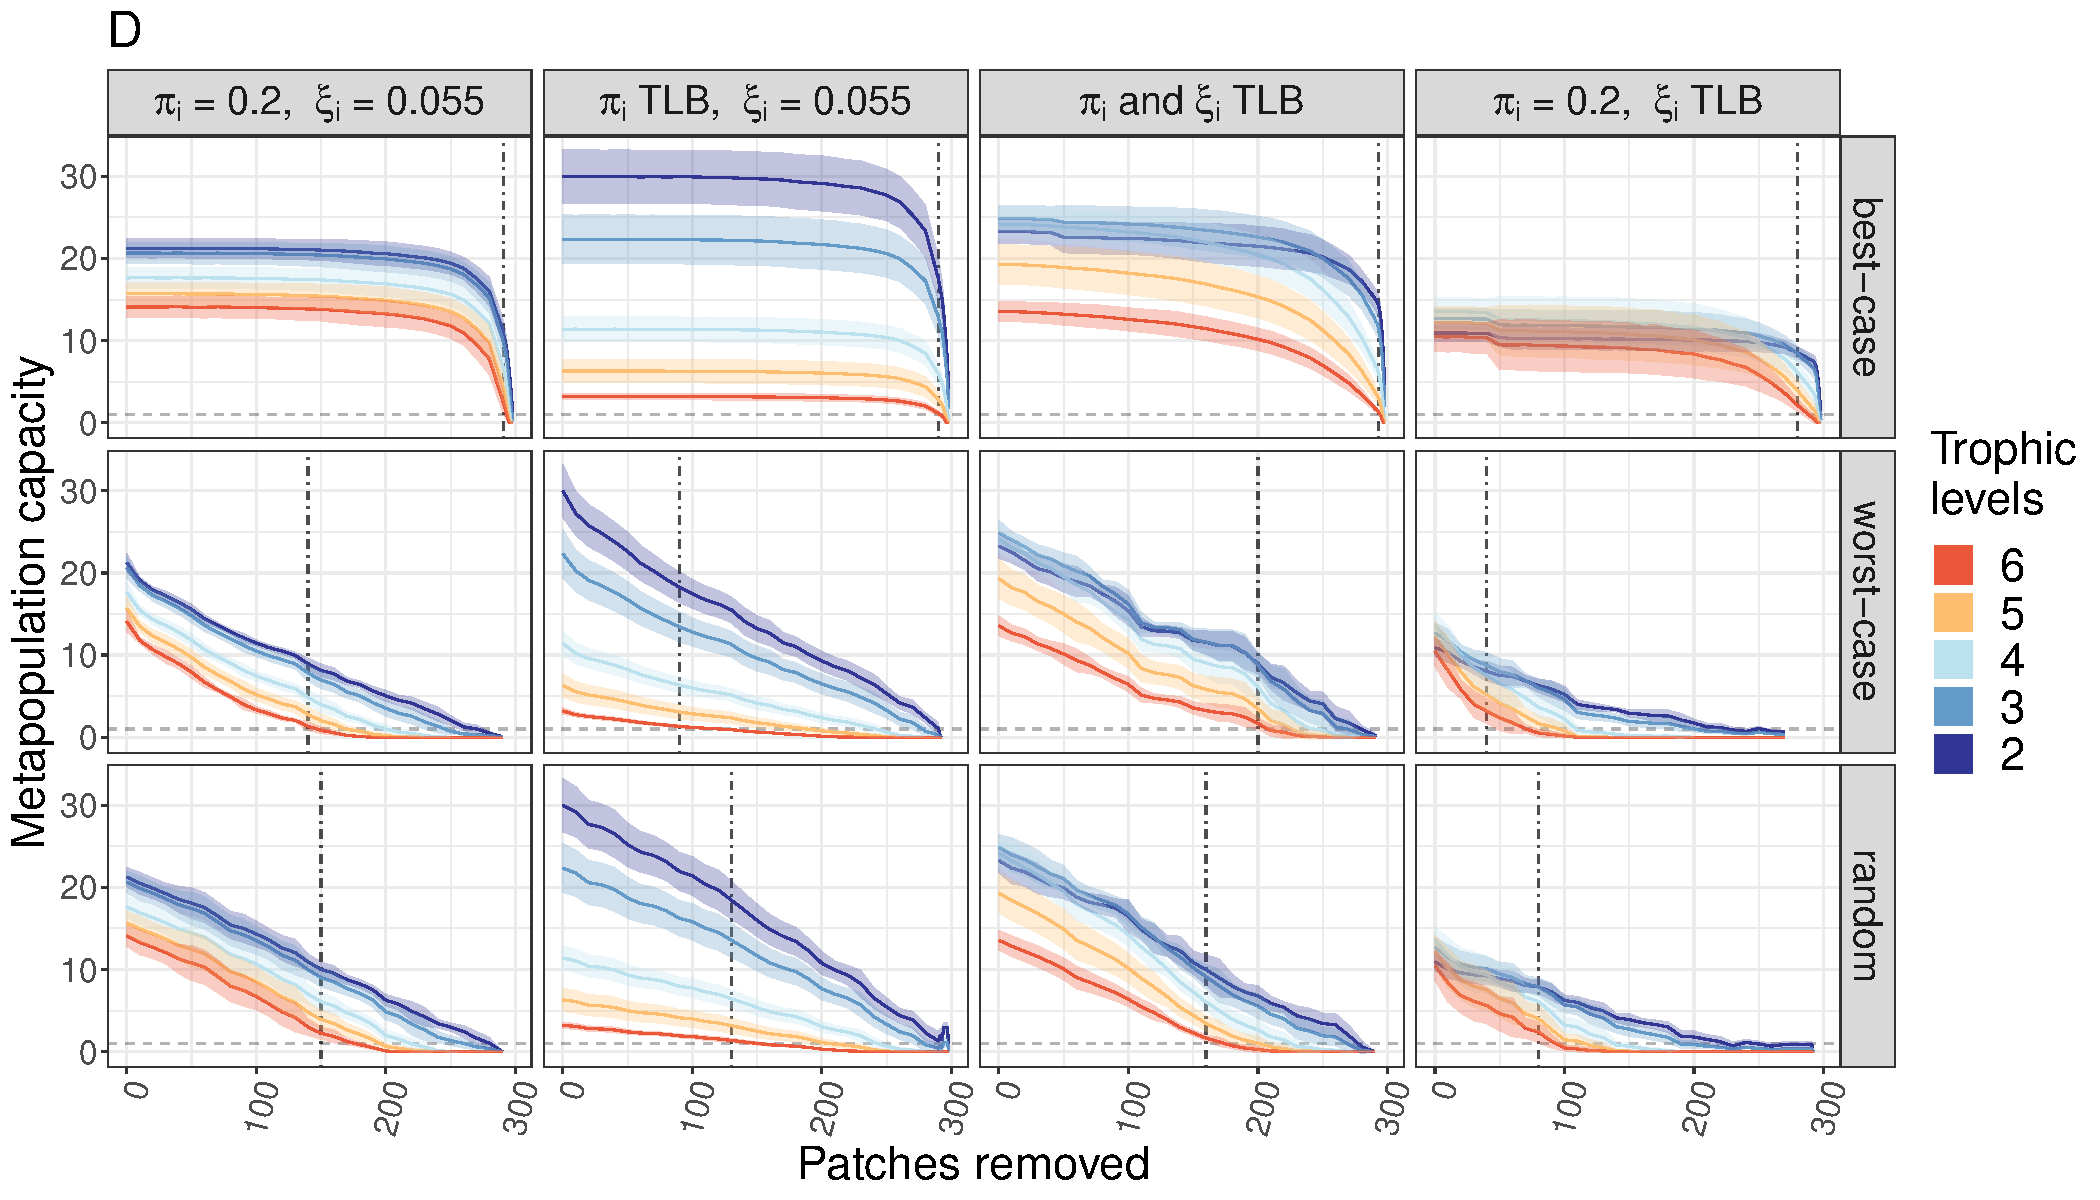
\includegraphics[width=0.8\textwidth,valign=t]{lambda_Model_food_web_with_250_consumer_and_150_basal_species_basal_5_5.pdf}
  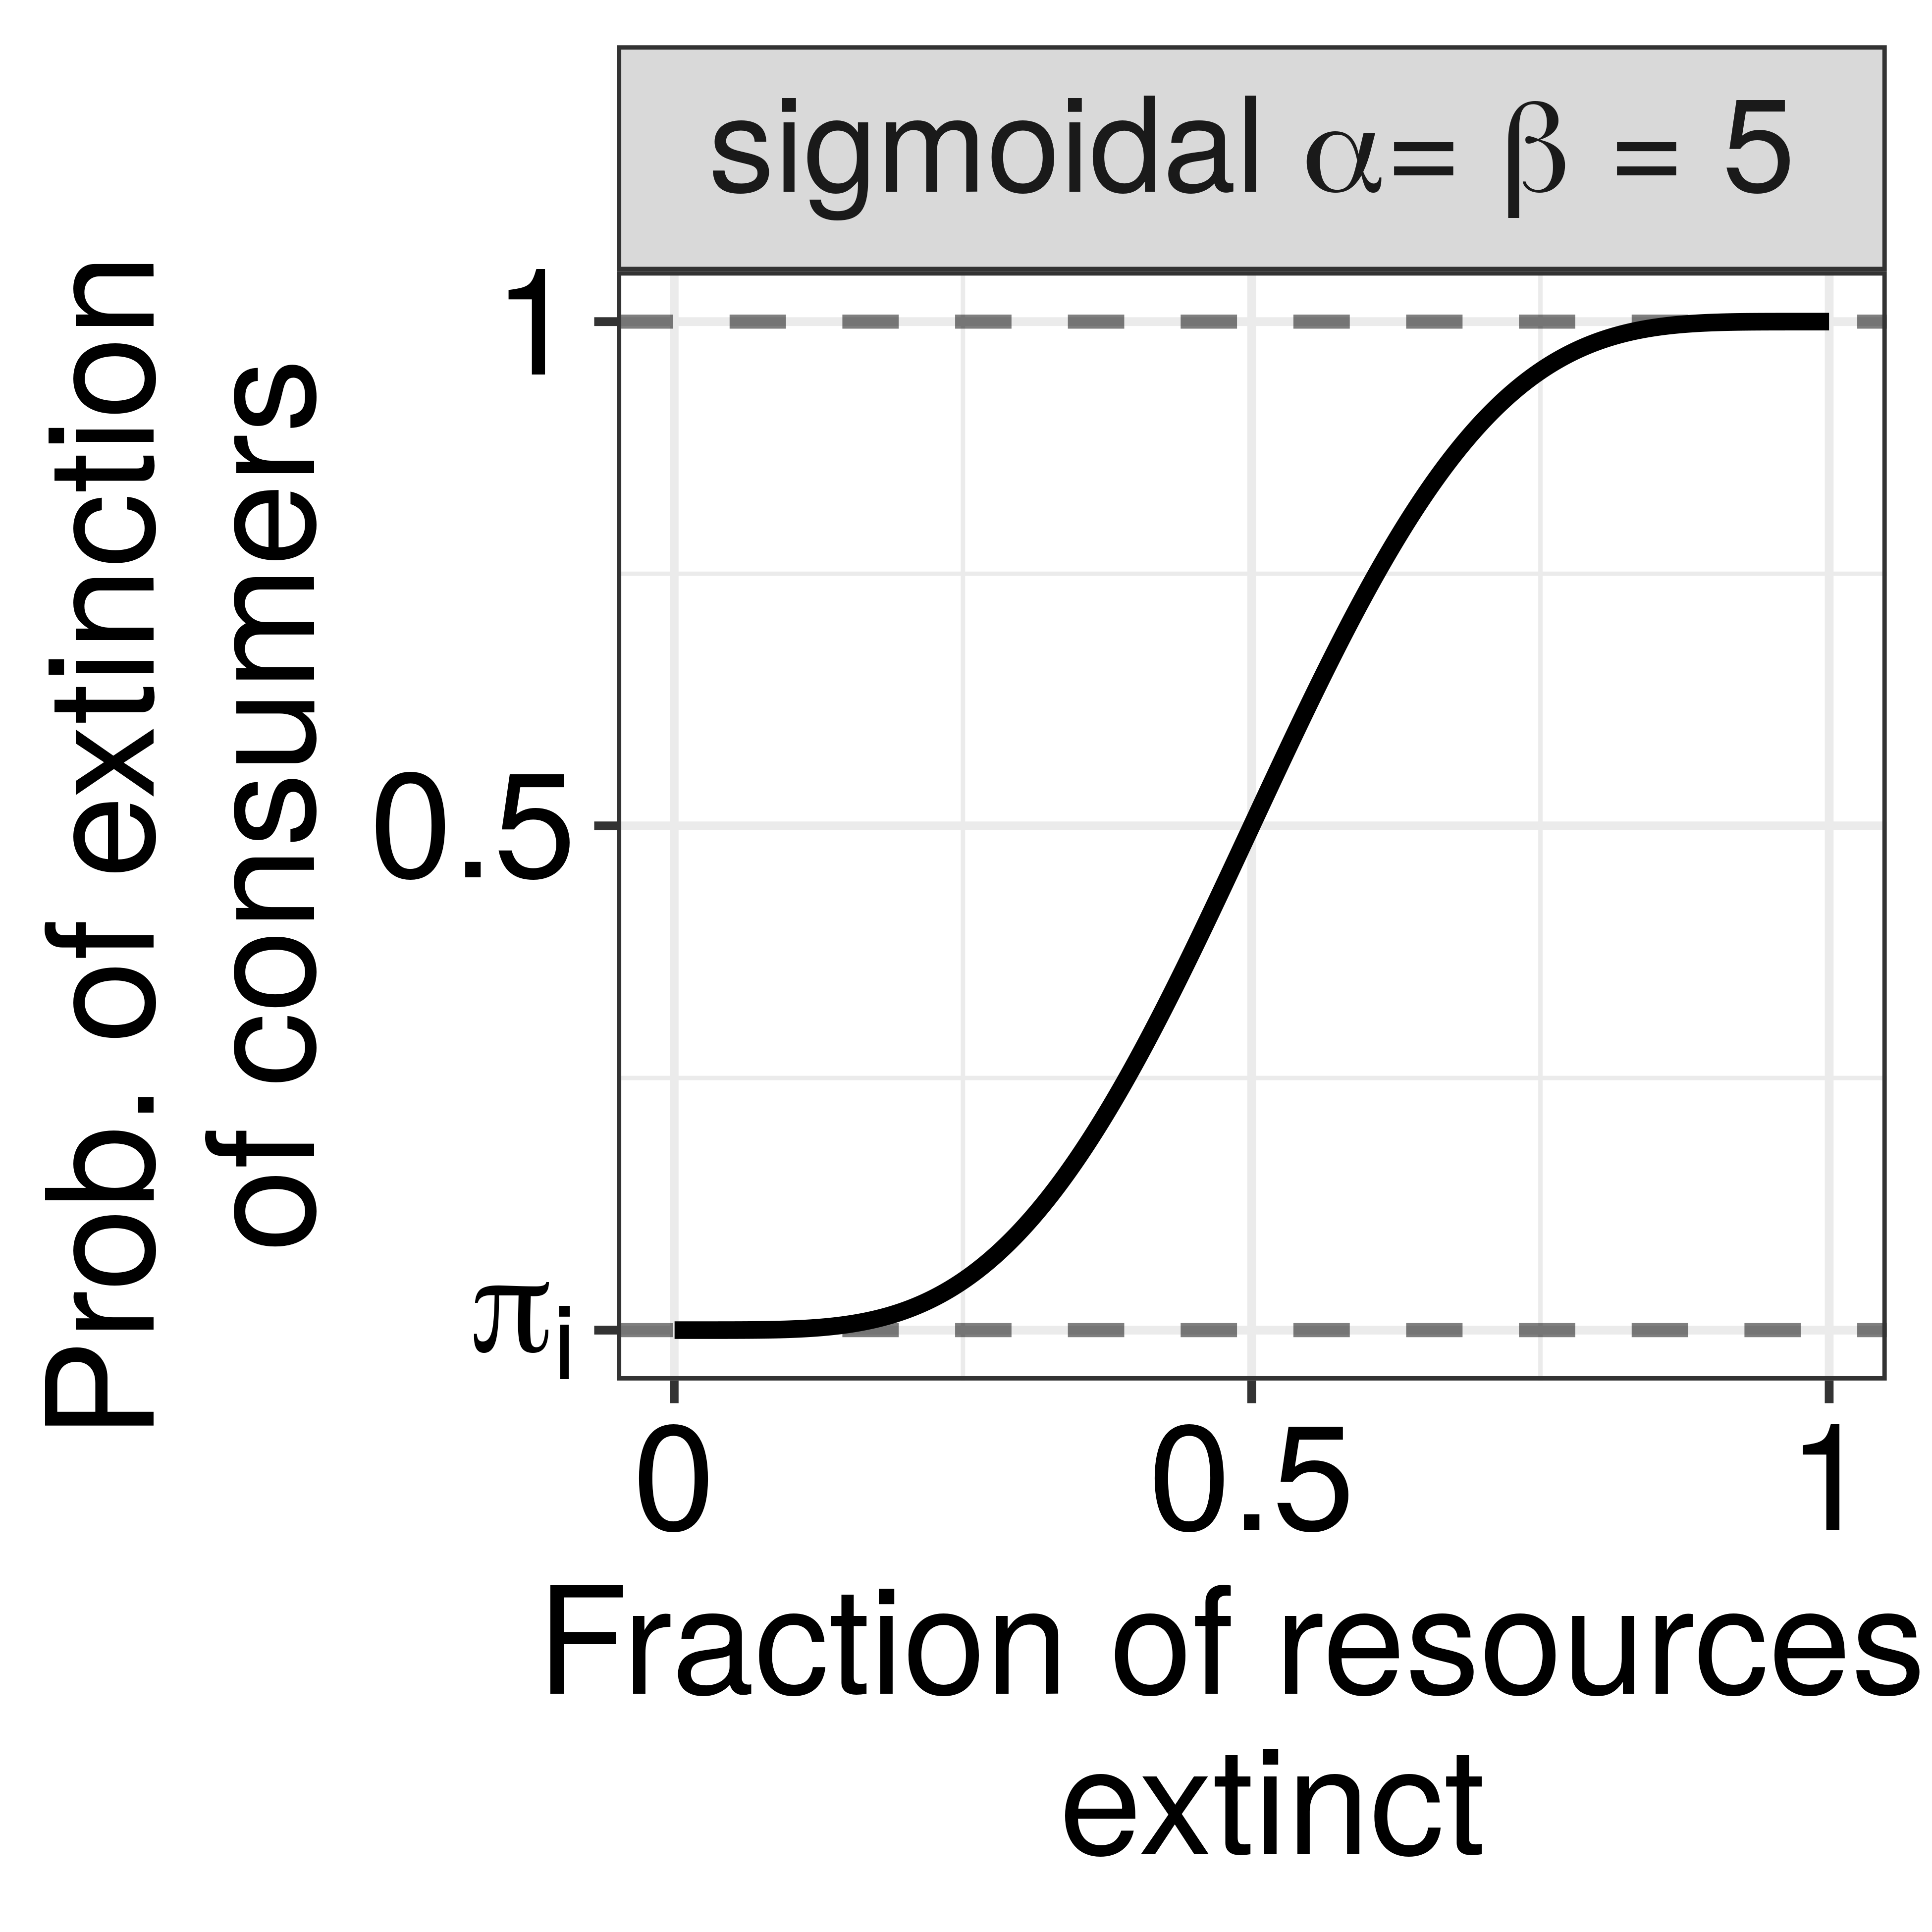
\includegraphics[width=0.19\textwidth,valign=t]{fform_5_5.png}
 \caption{Figure continued.}
 \label{S_fig:patchloss_250_150_2}
\end{figure}

\begin{figure}
  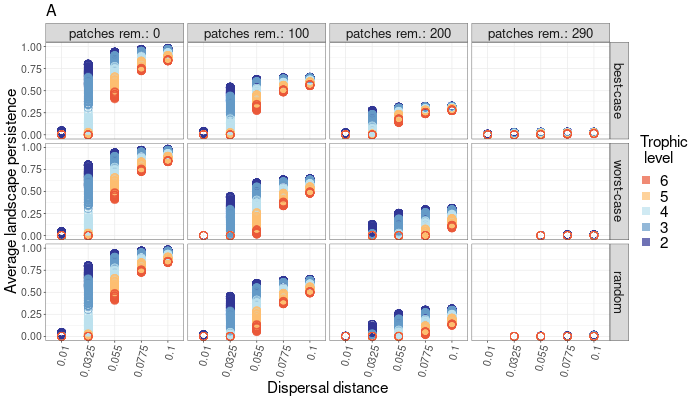
\includegraphics[width=0.8\textwidth,valign=t]{sump_Model_food_web_with_250_consumer_and_150_basal_species_basal_1_1.png}
  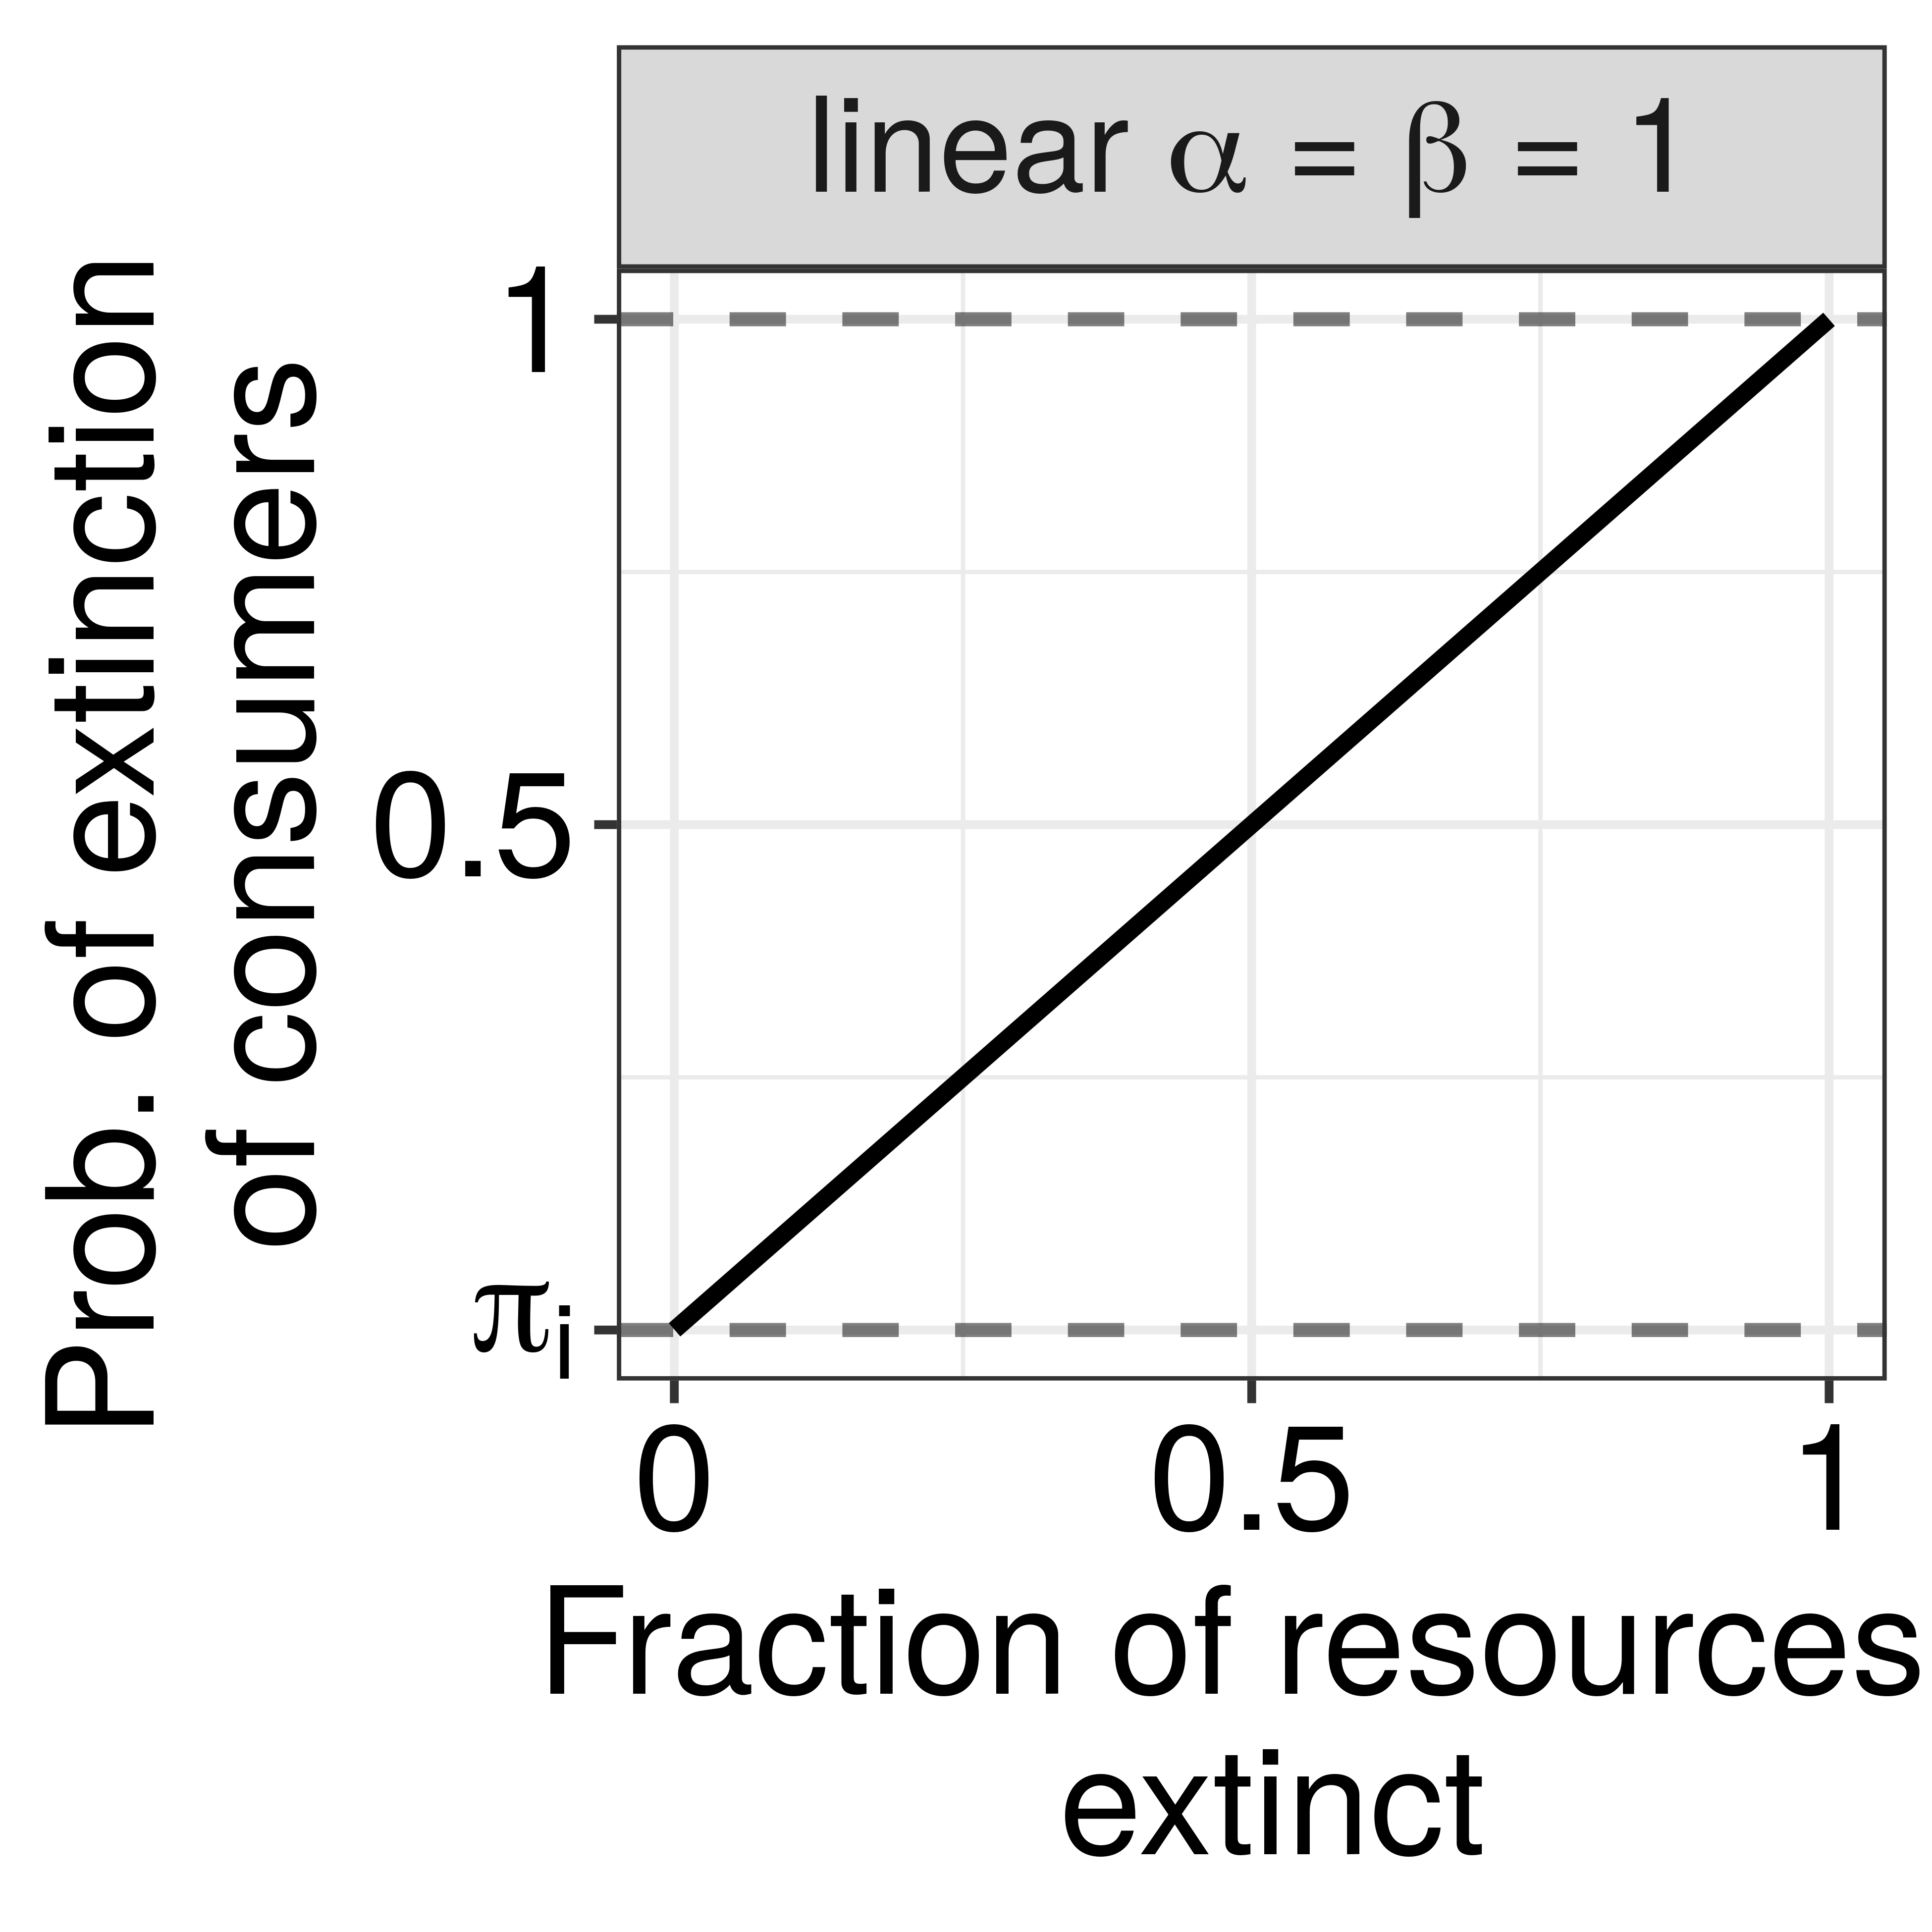
\includegraphics[width=0.19\textwidth,valign=t]{fform_1_1.png}
  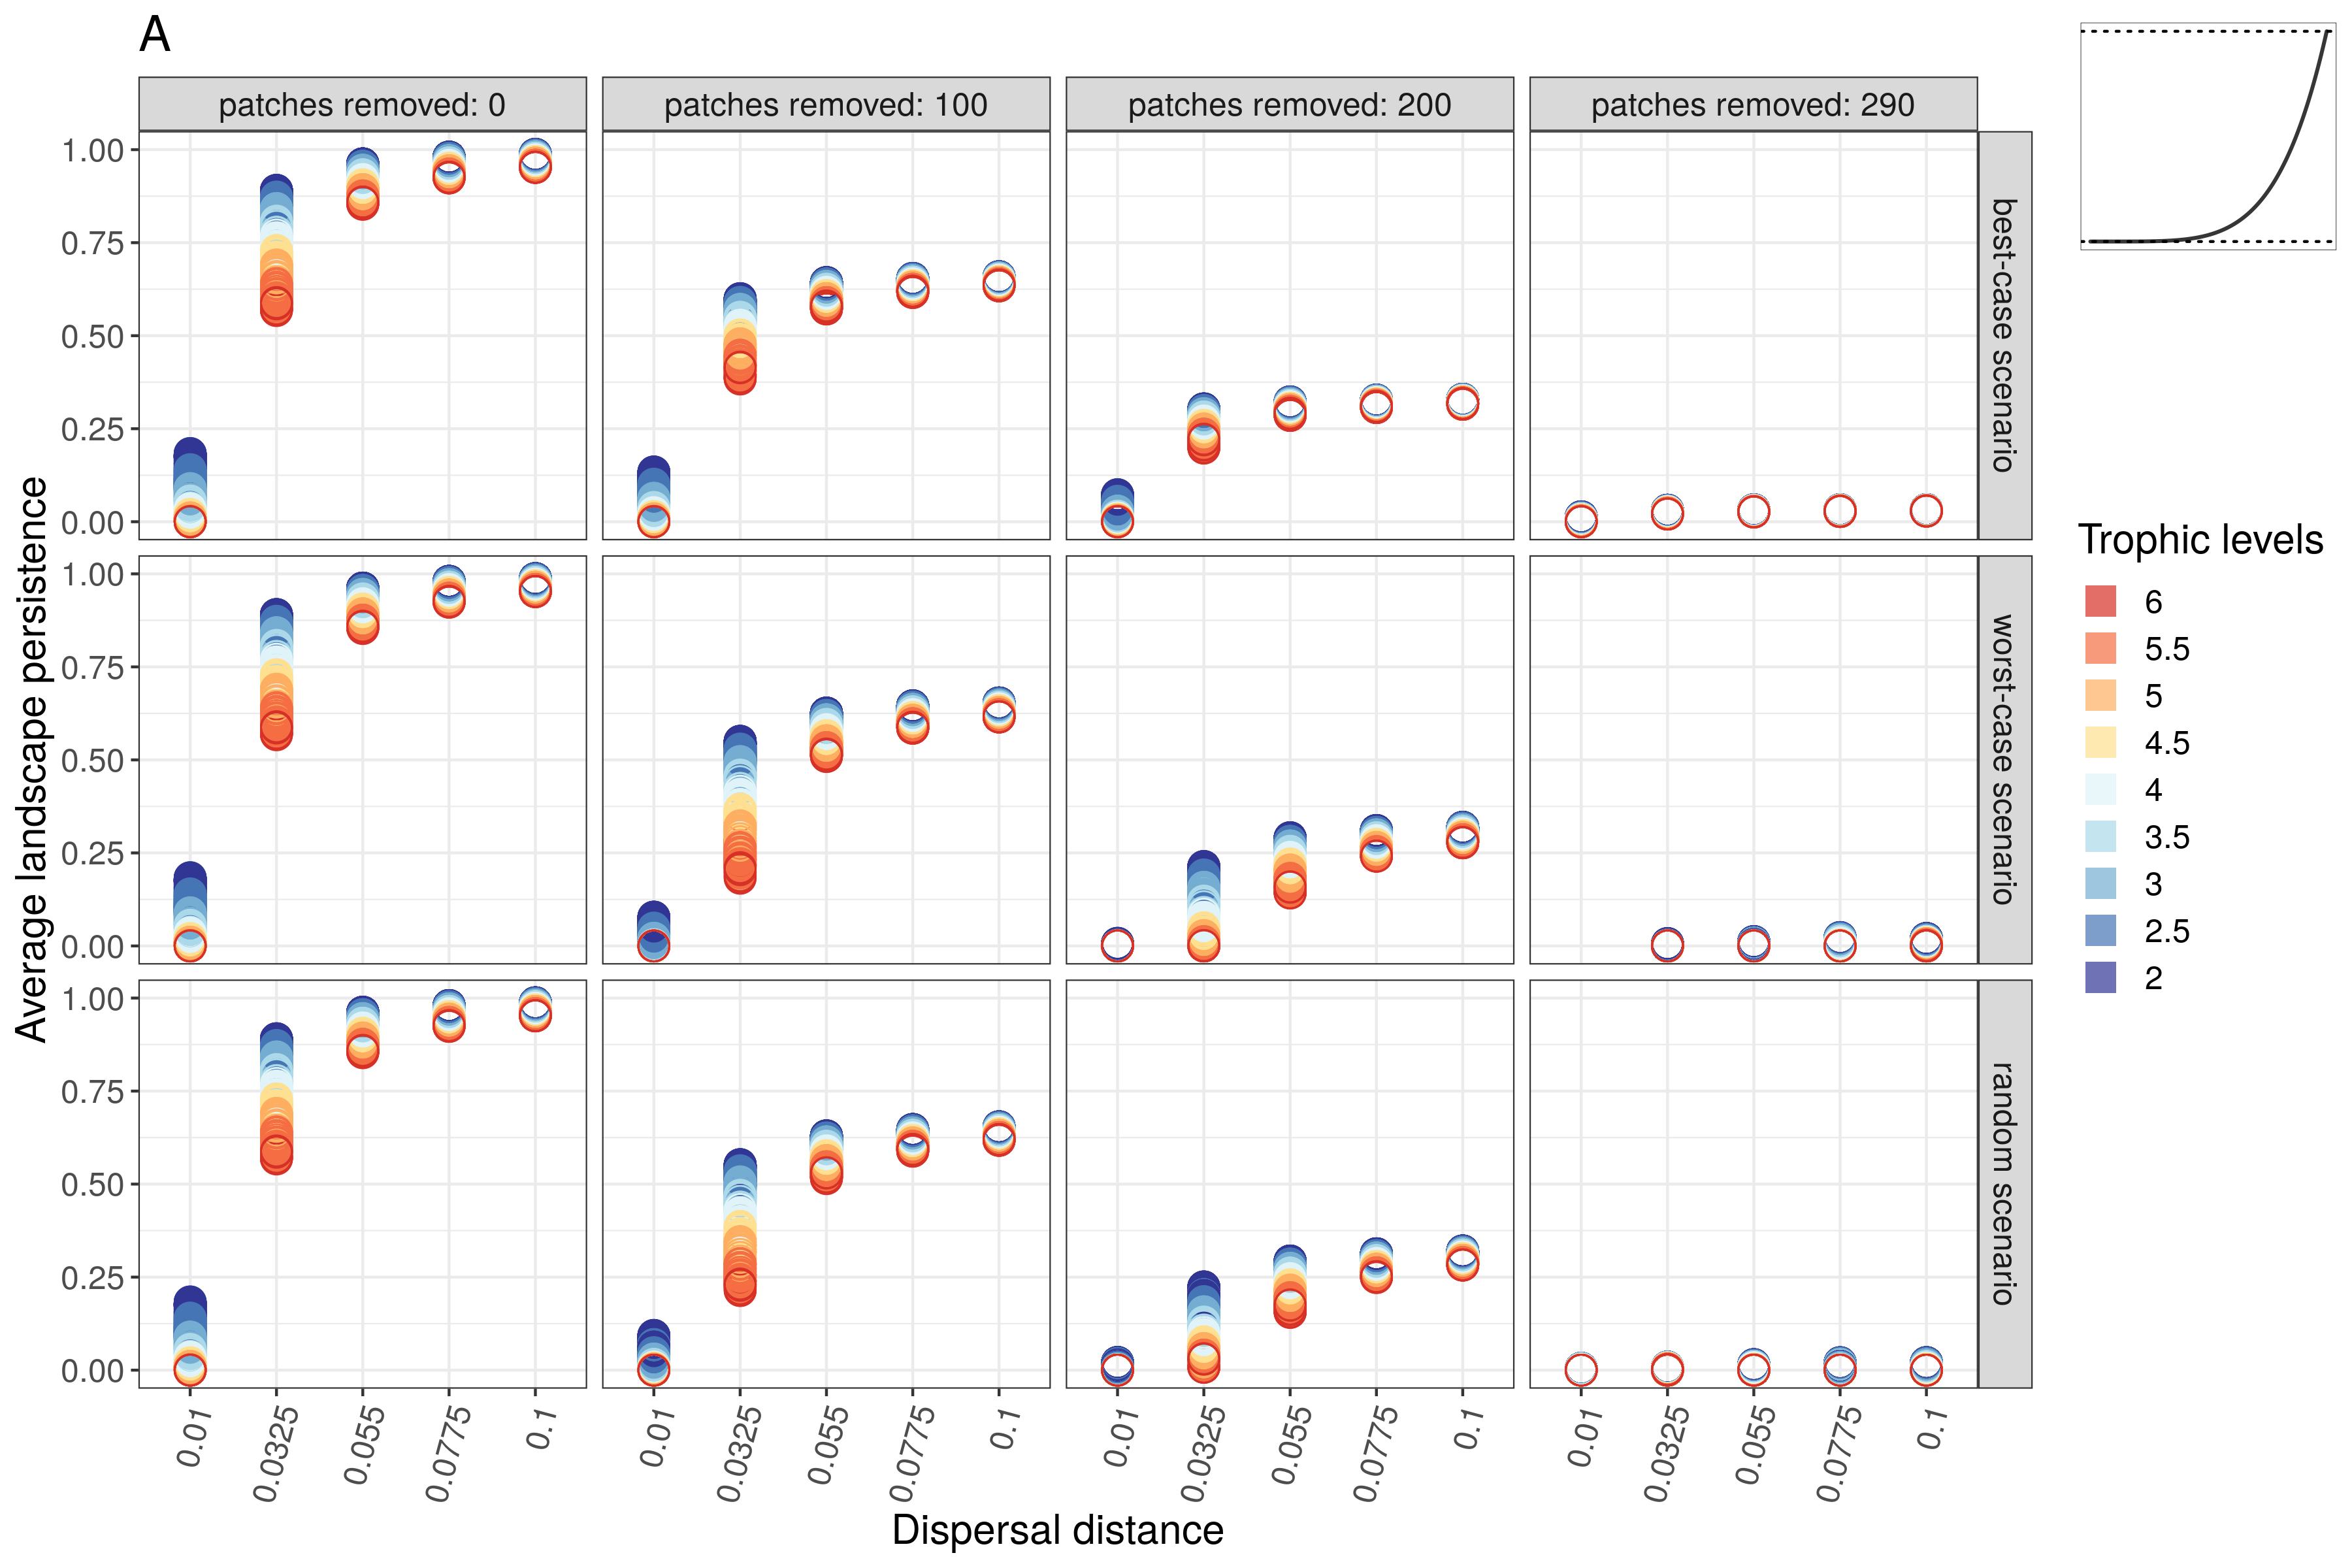
\includegraphics[width=0.8\textwidth,valign=t]{sump_Model_food_web_with_250_consumer_and_150_basal_species_basal_5_1.png}
    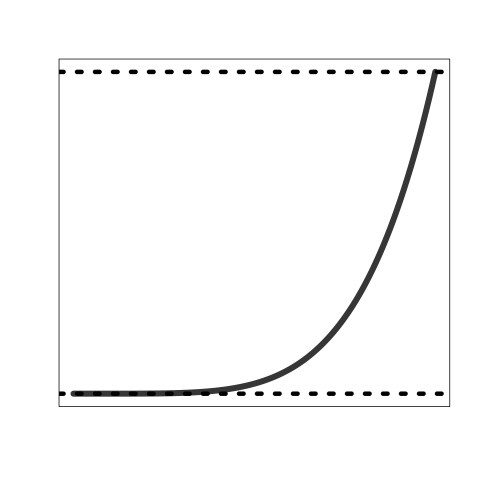
\includegraphics[width=0.19\textwidth,valign=t]{fform_5_1.png}
 \caption{As Figure \ref{S_fig:patchloss_300_100_distance_1}, but with 250 consumer and 150 basal species.} 
 \label{S_fig:patchloss_250_150_distance_1}
\end{figure}

\begin{figure}\ContinuedFloat
  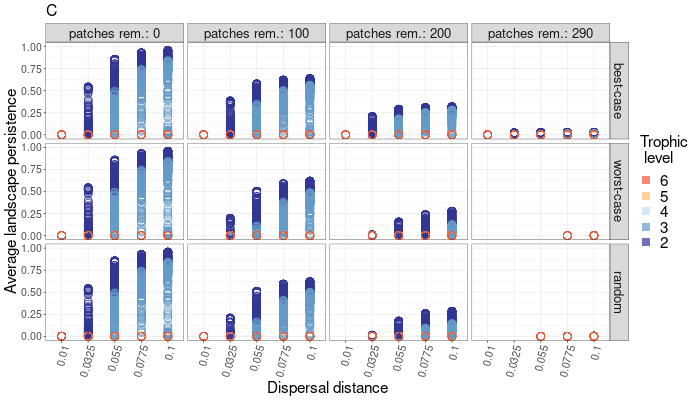
\includegraphics[width=0.8\textwidth,valign=t]{sump_Model_food_web_with_250_consumer_and_150_basal_species_basal_1_5.png}
  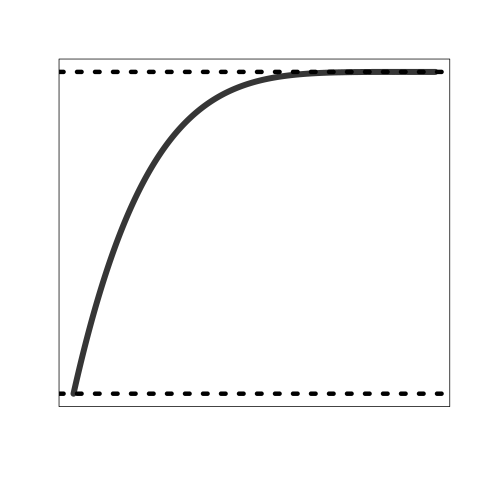
\includegraphics[width=0.19\textwidth,valign=t]{fform_1_5.png}
  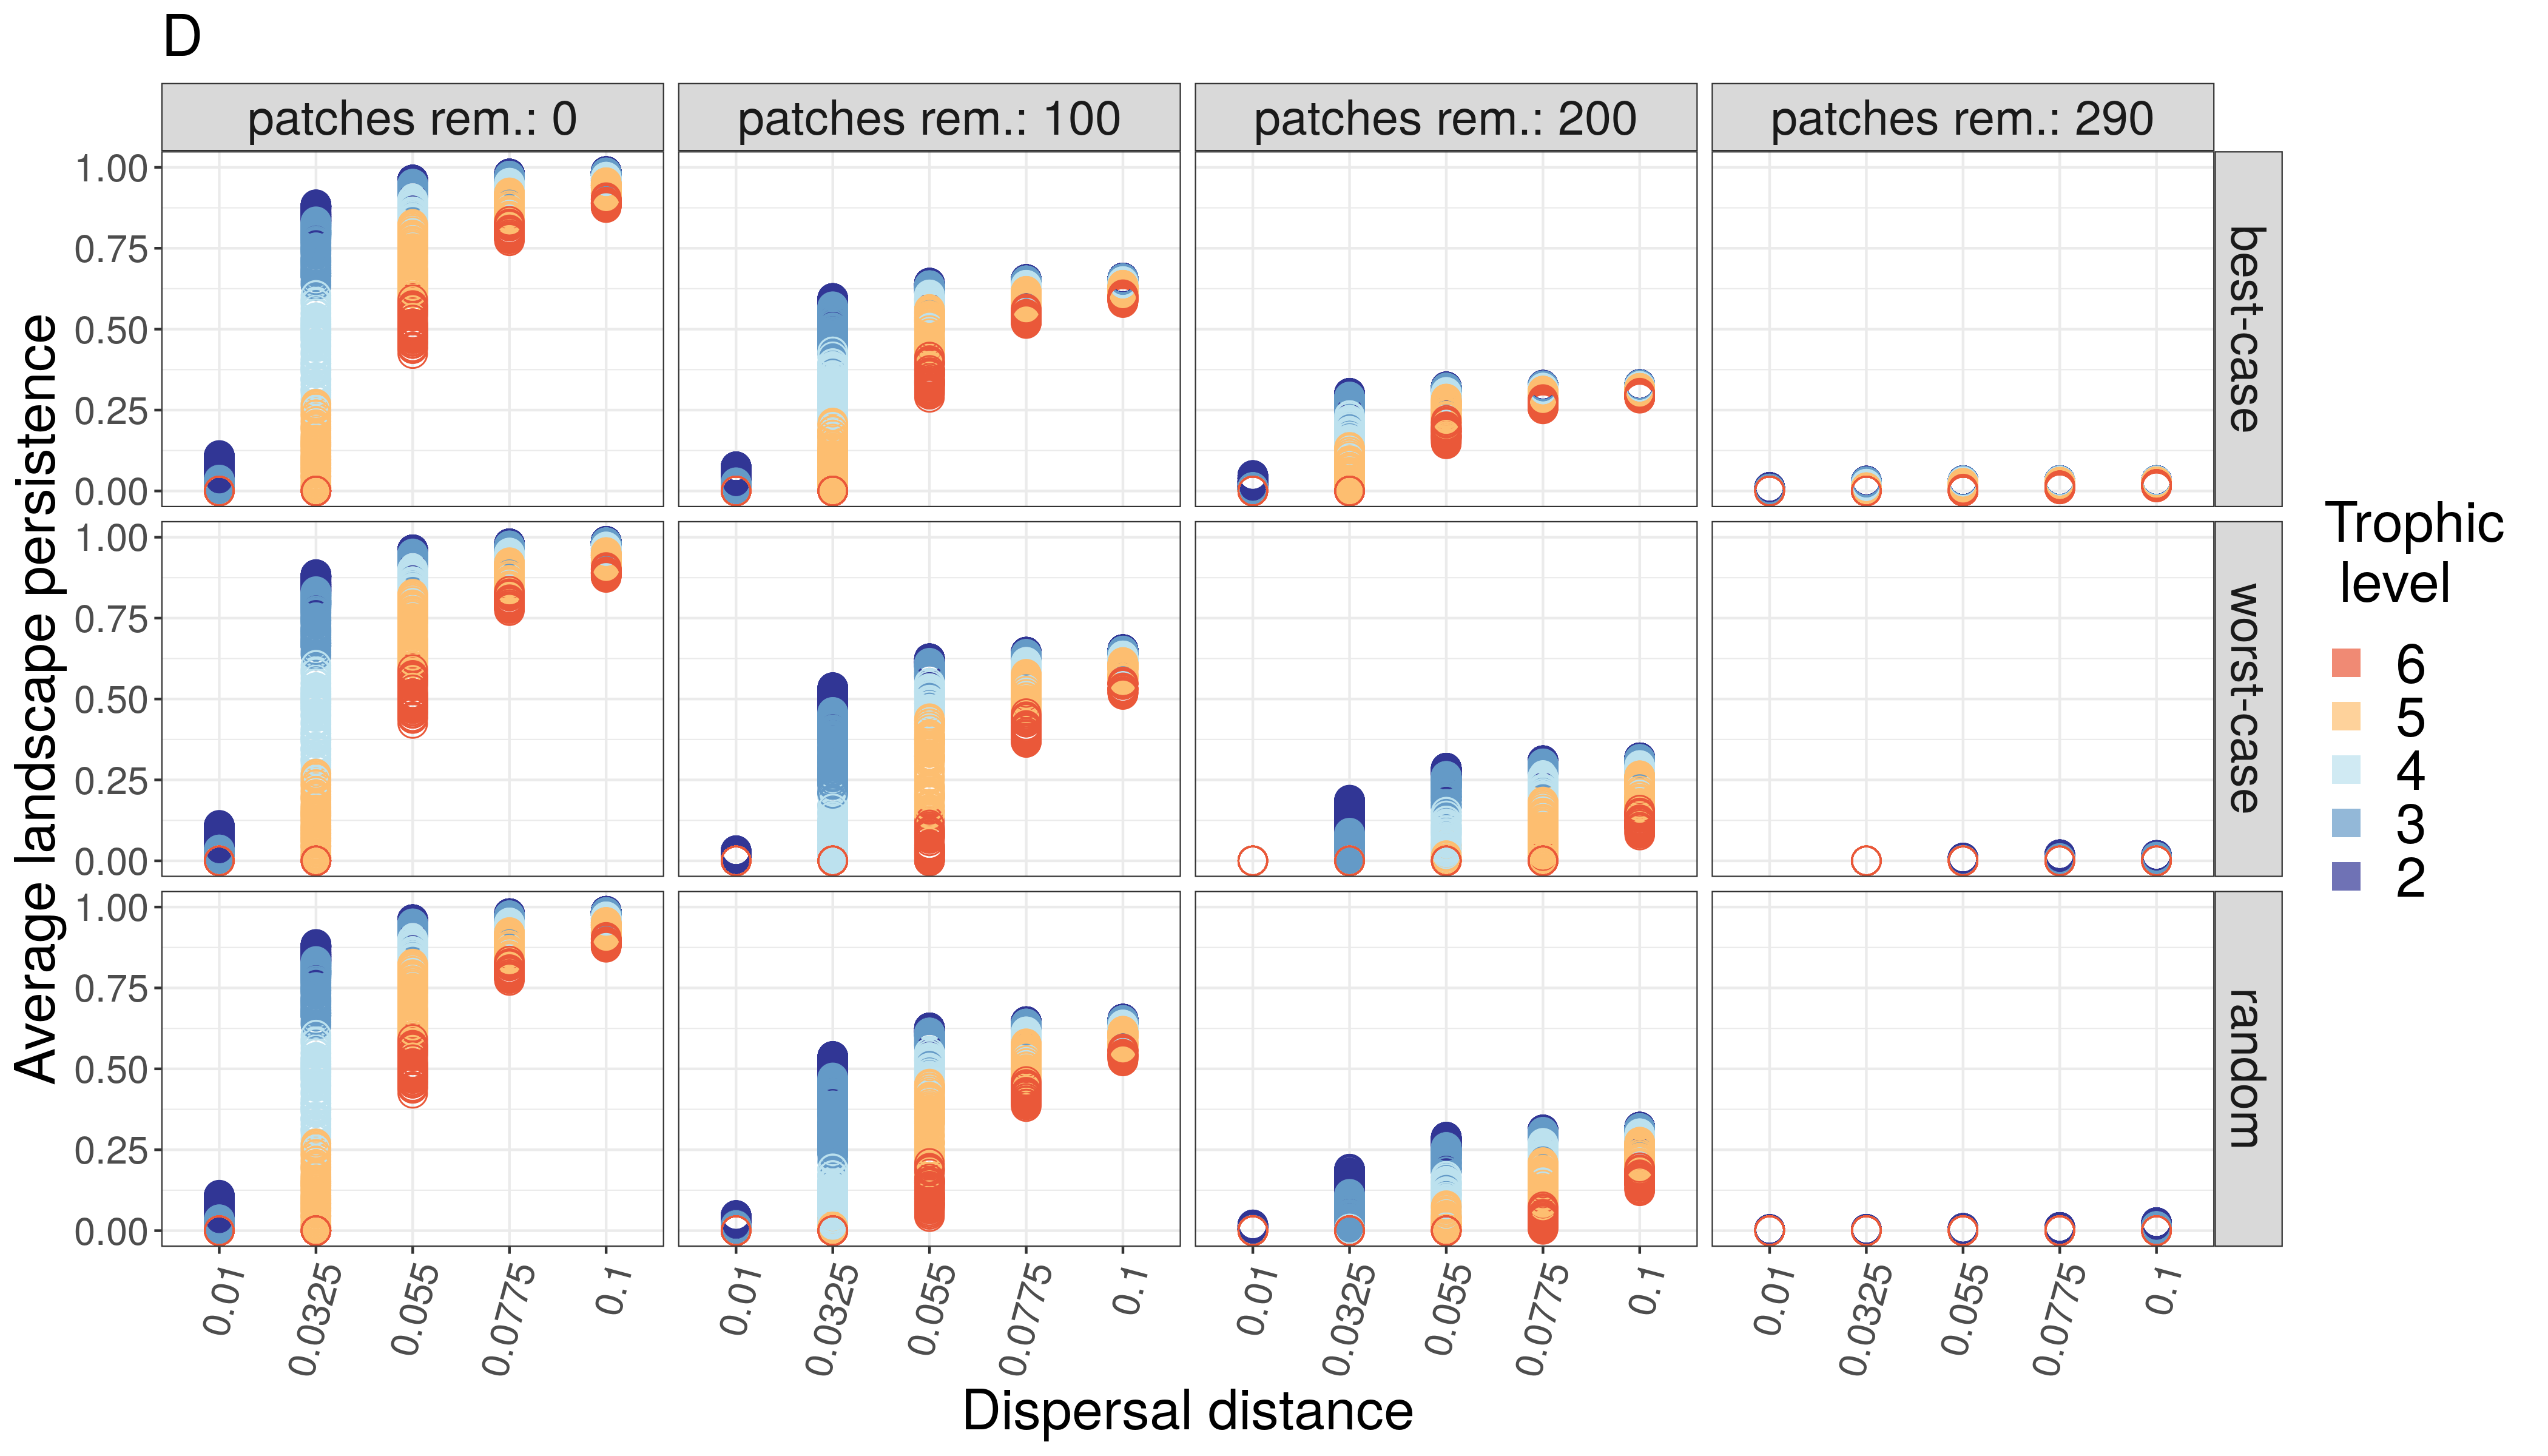
\includegraphics[width=0.8\textwidth,valign=t]{sump_Model_food_web_with_250_consumer_and_150_basal_species_basal_5_5.png}
  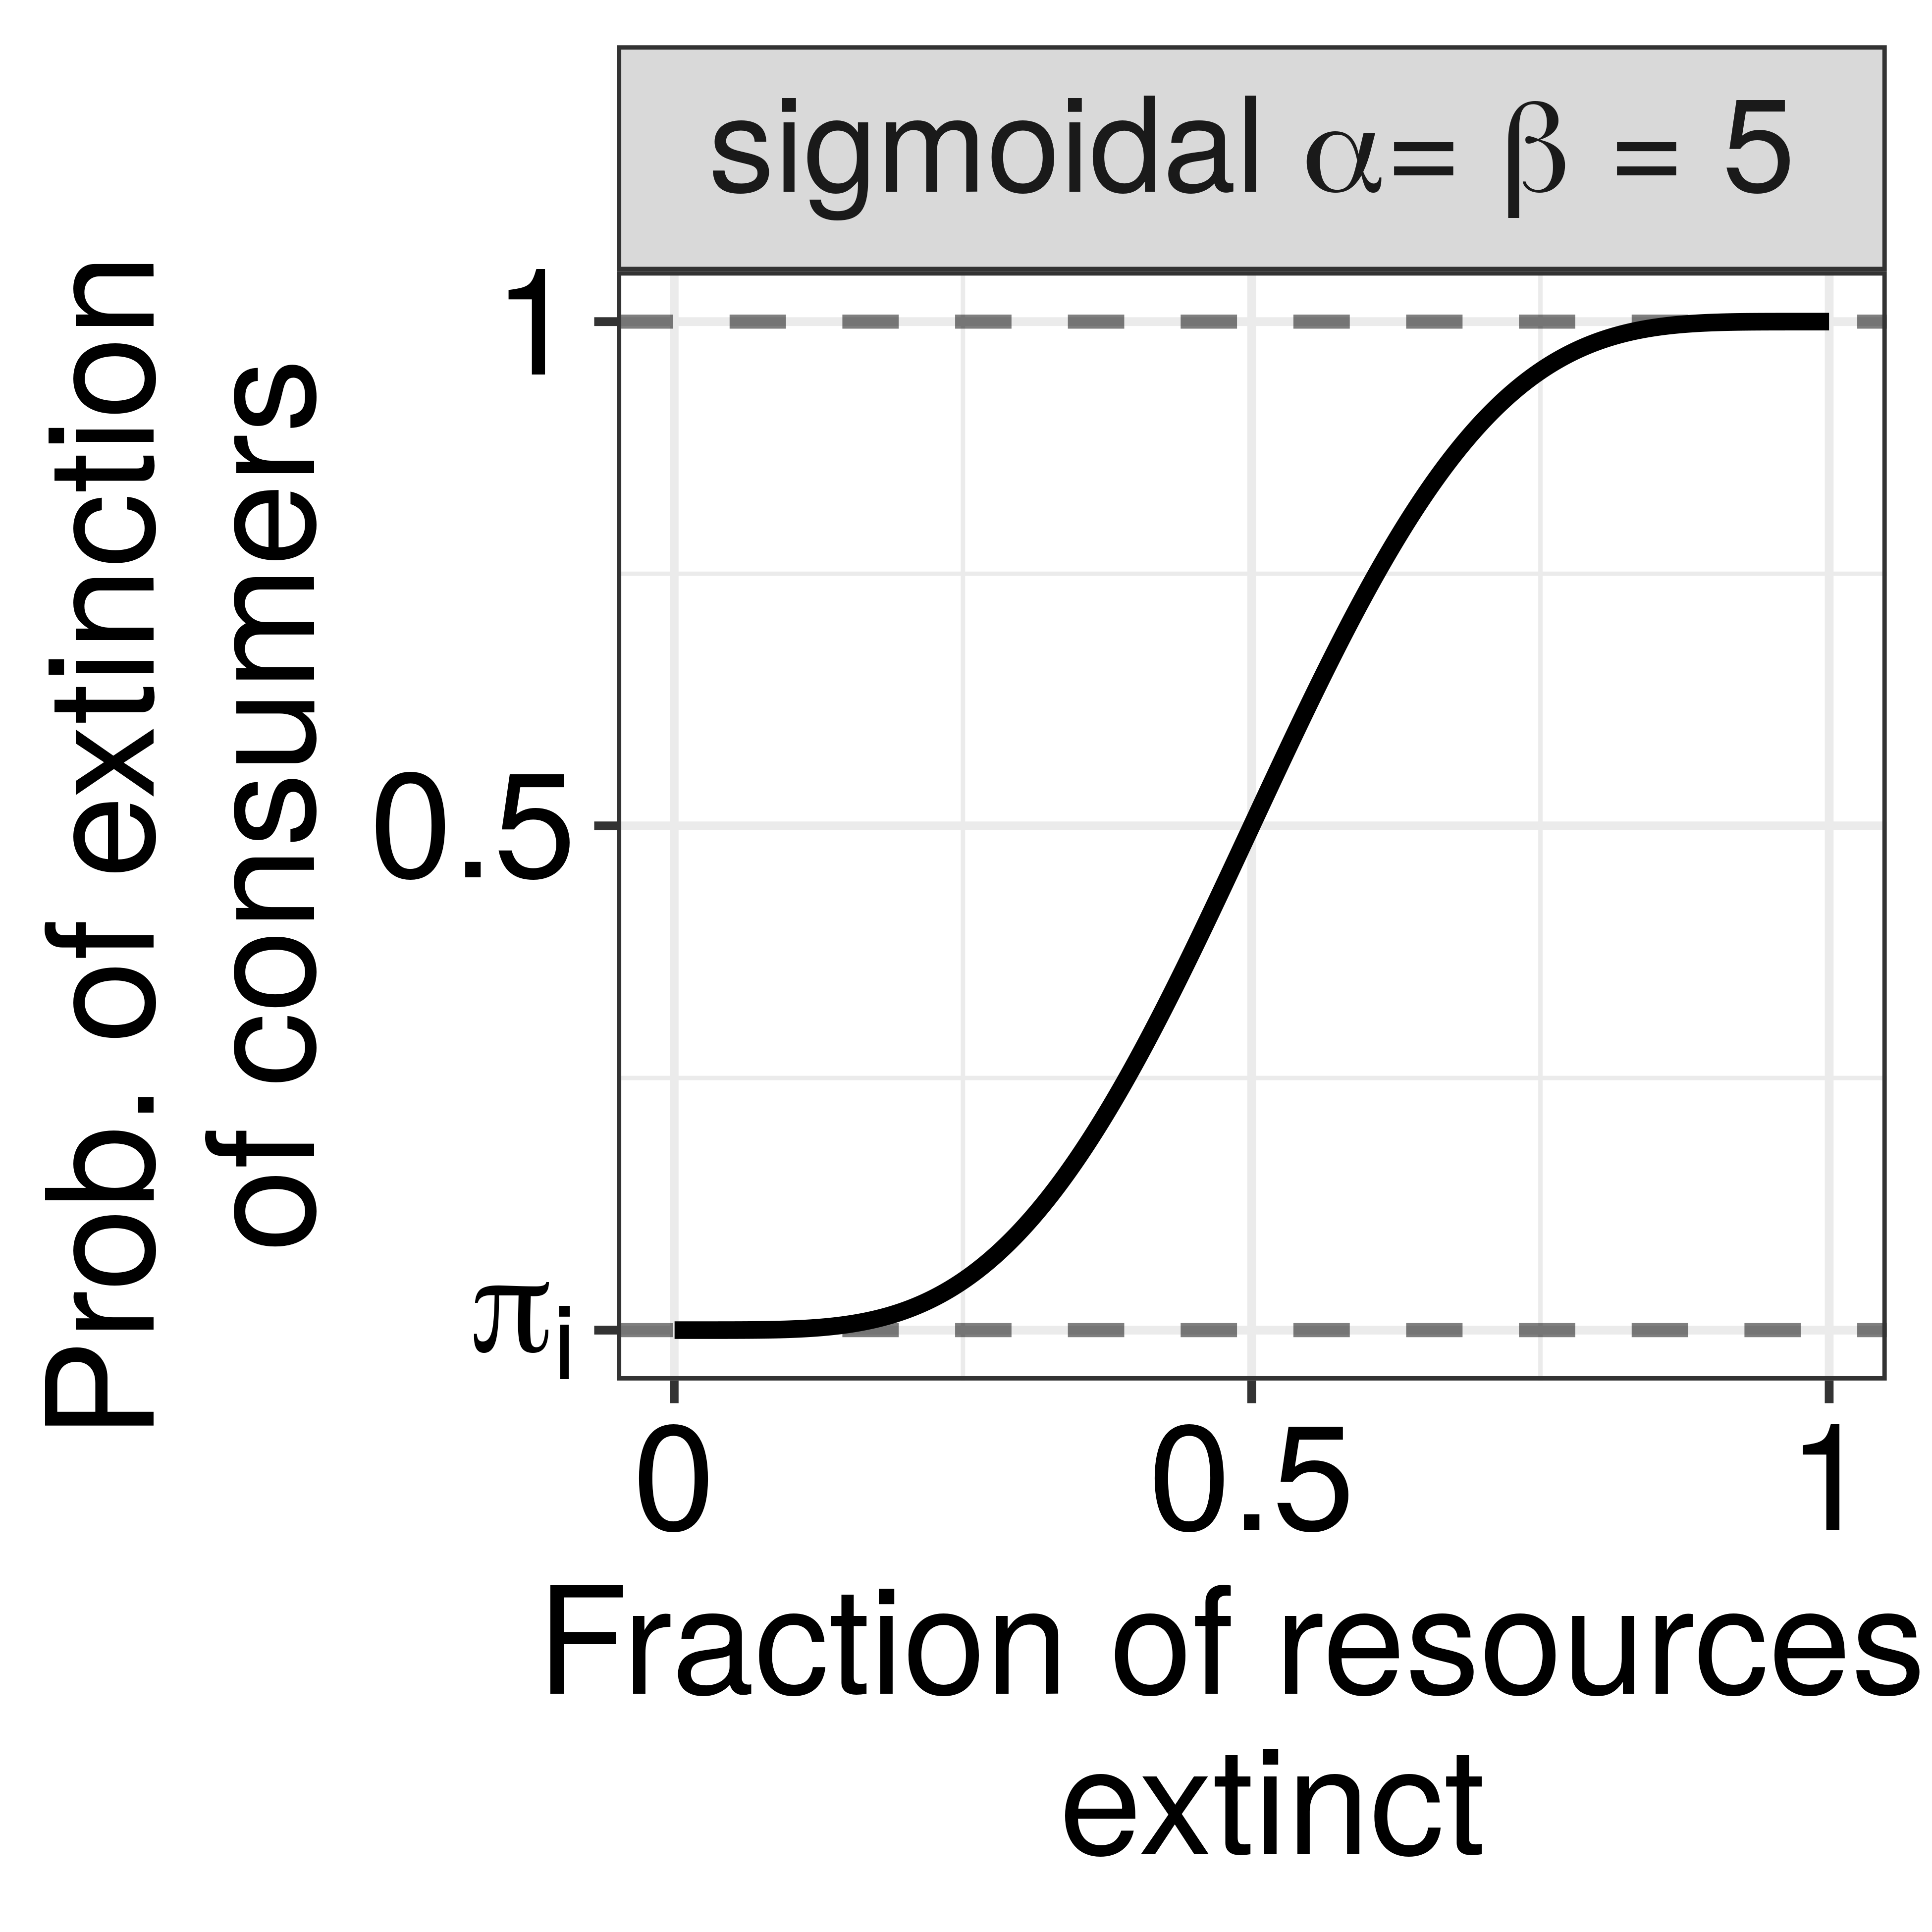
\includegraphics[width=0.19\textwidth,valign=t]{fform_5_5.png}
 \caption{Figure continued.}
 \label{S_fig:patchloss_250_150_distance_2}
\end{figure}

\begin{figure}[!ht]
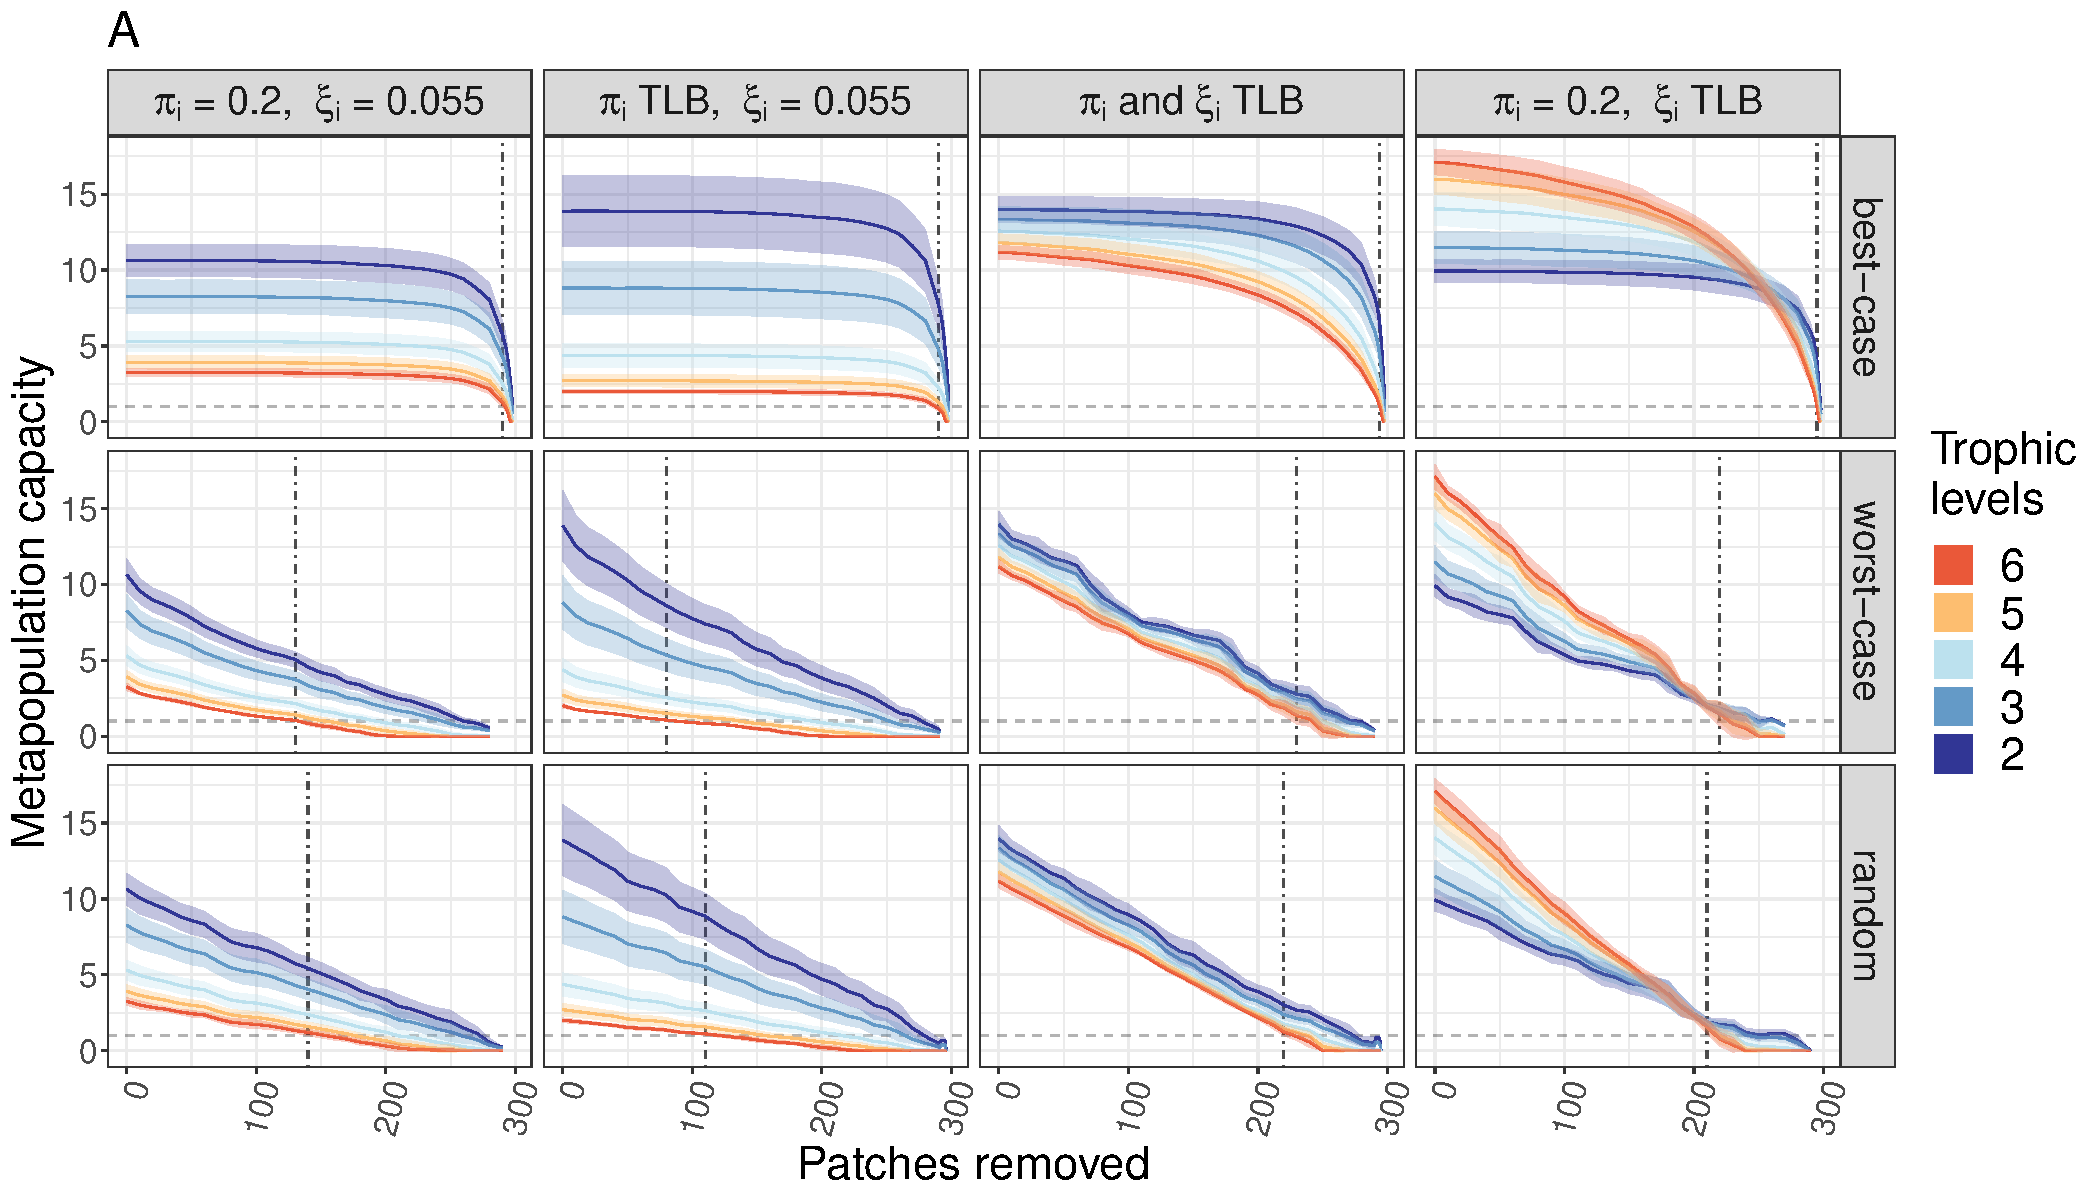
\includegraphics[width=0.8\textwidth,valign=t]{lambda_Model_food_web_with_200_consumer_and_200_basal_species_basal_1_1.pdf}
  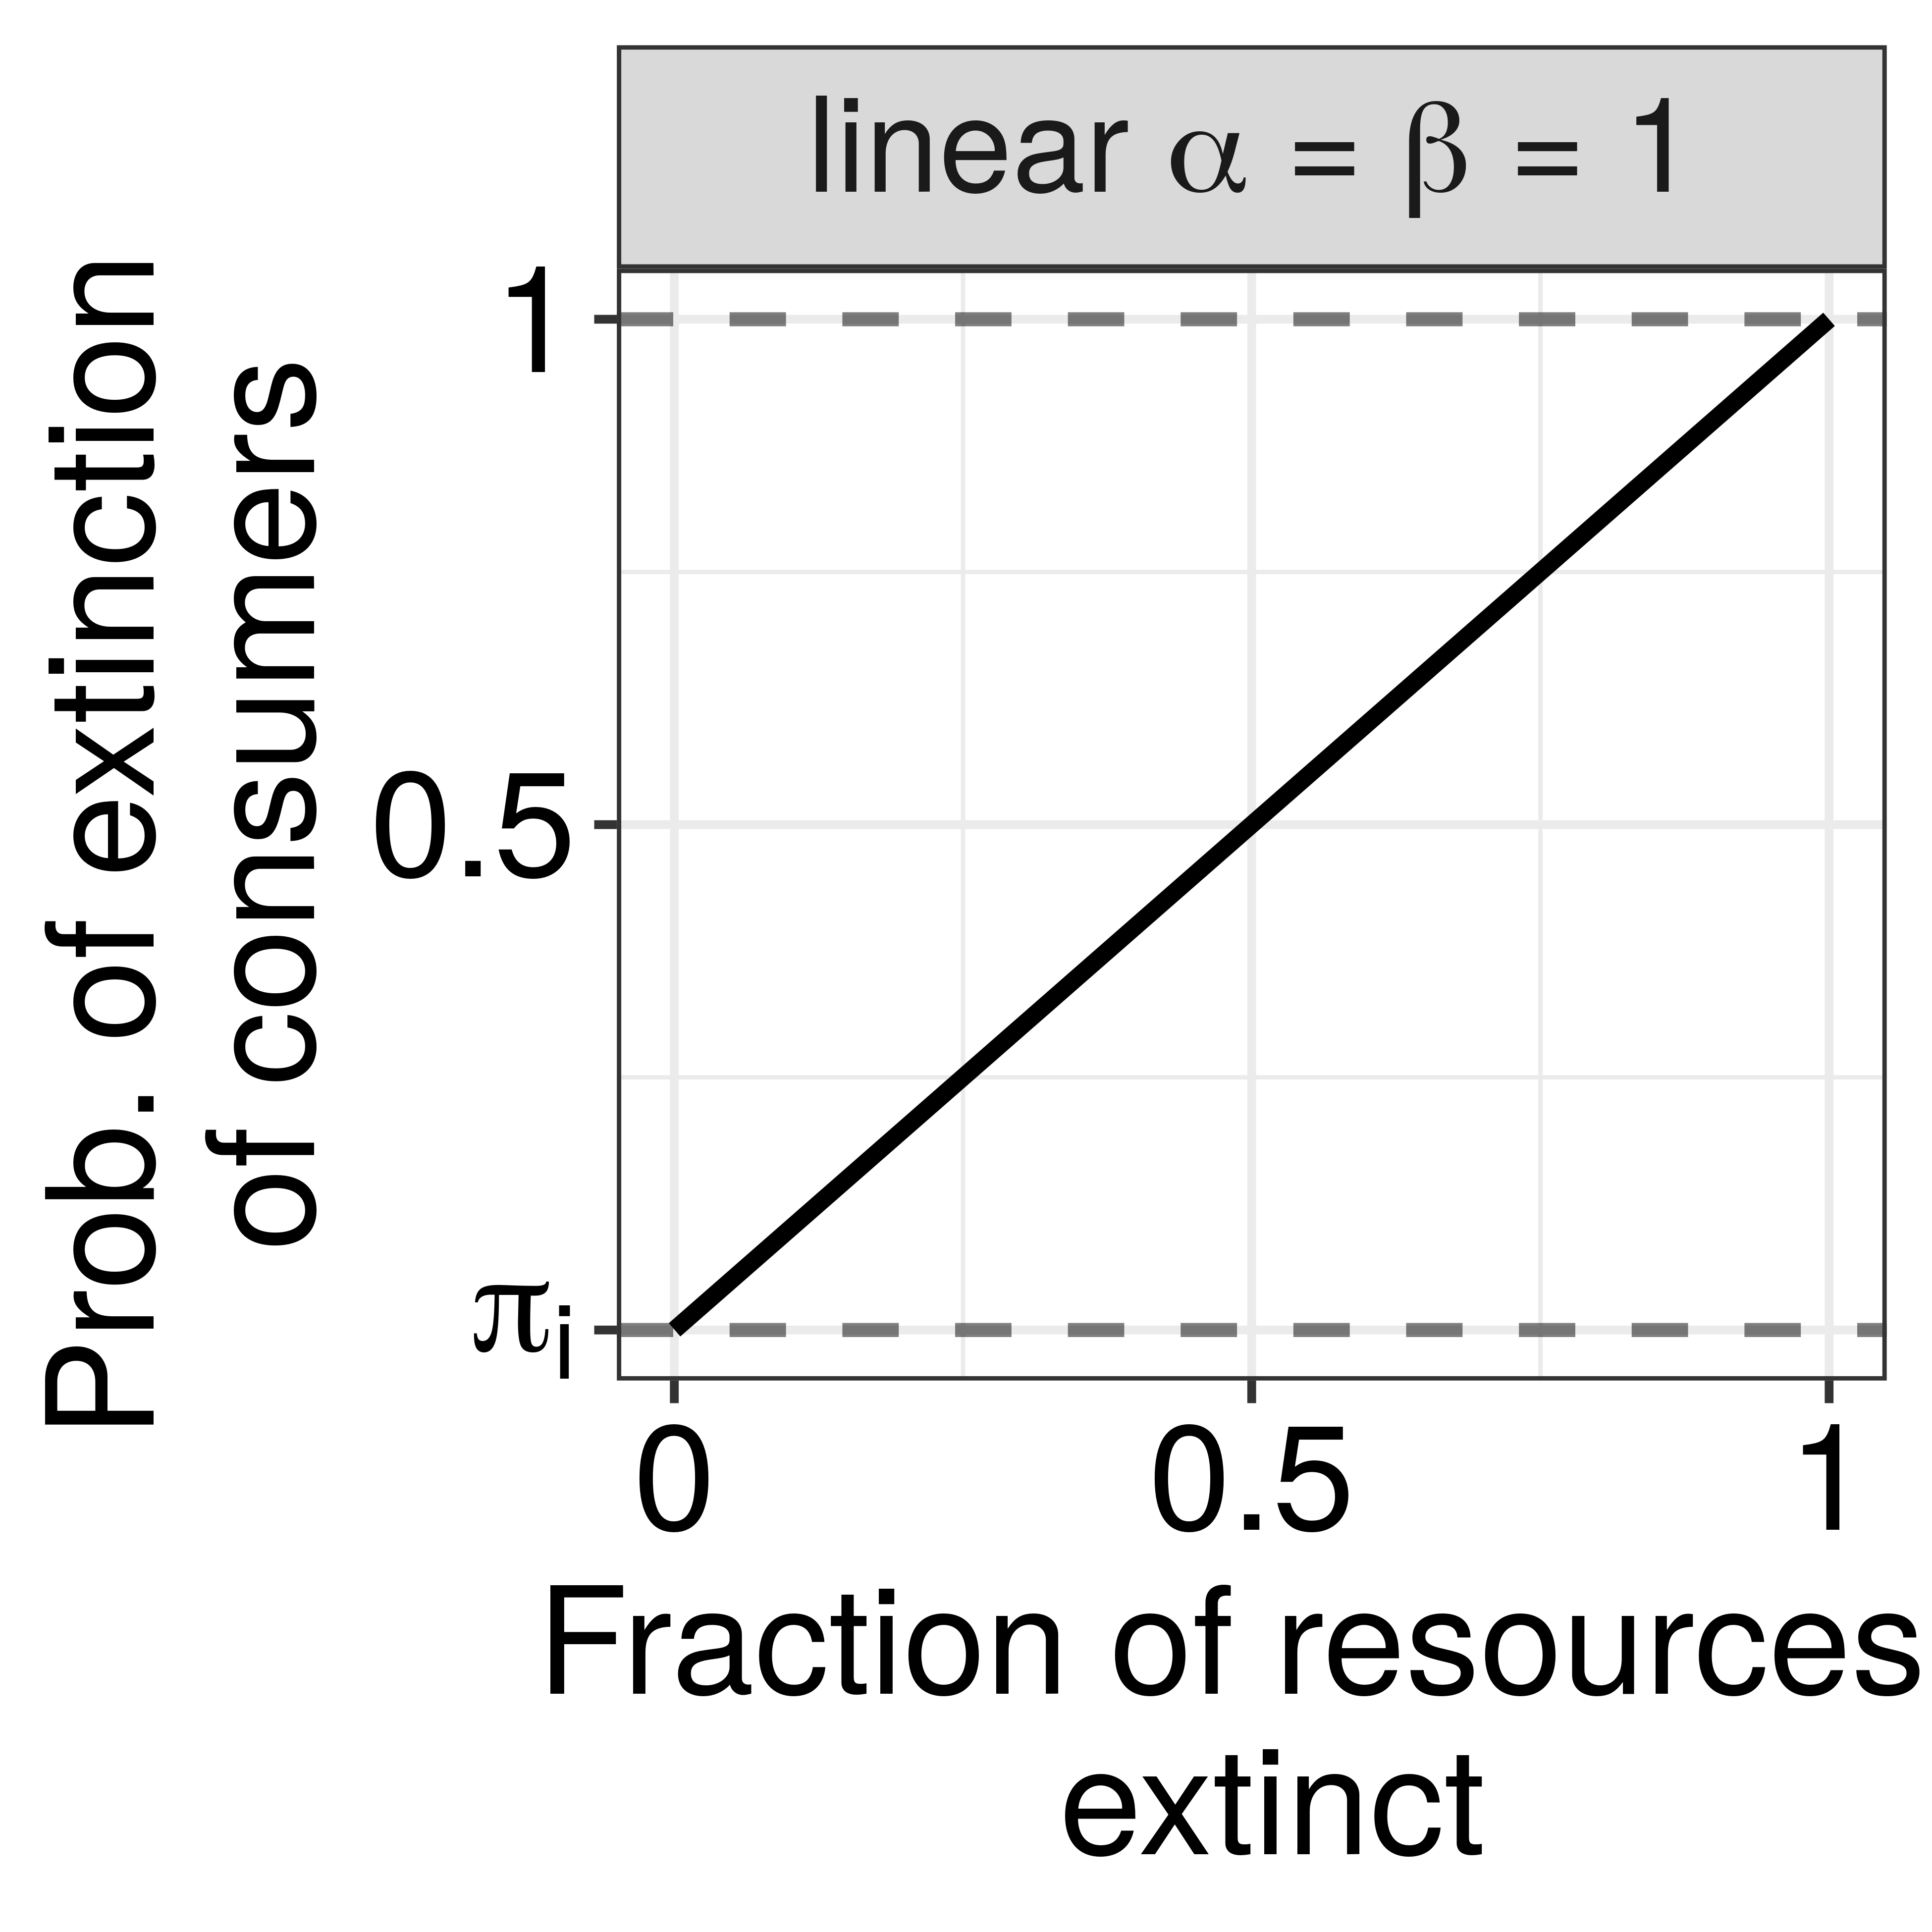
\includegraphics[width=0.19\textwidth,valign=t]{fform_1_1.png}
  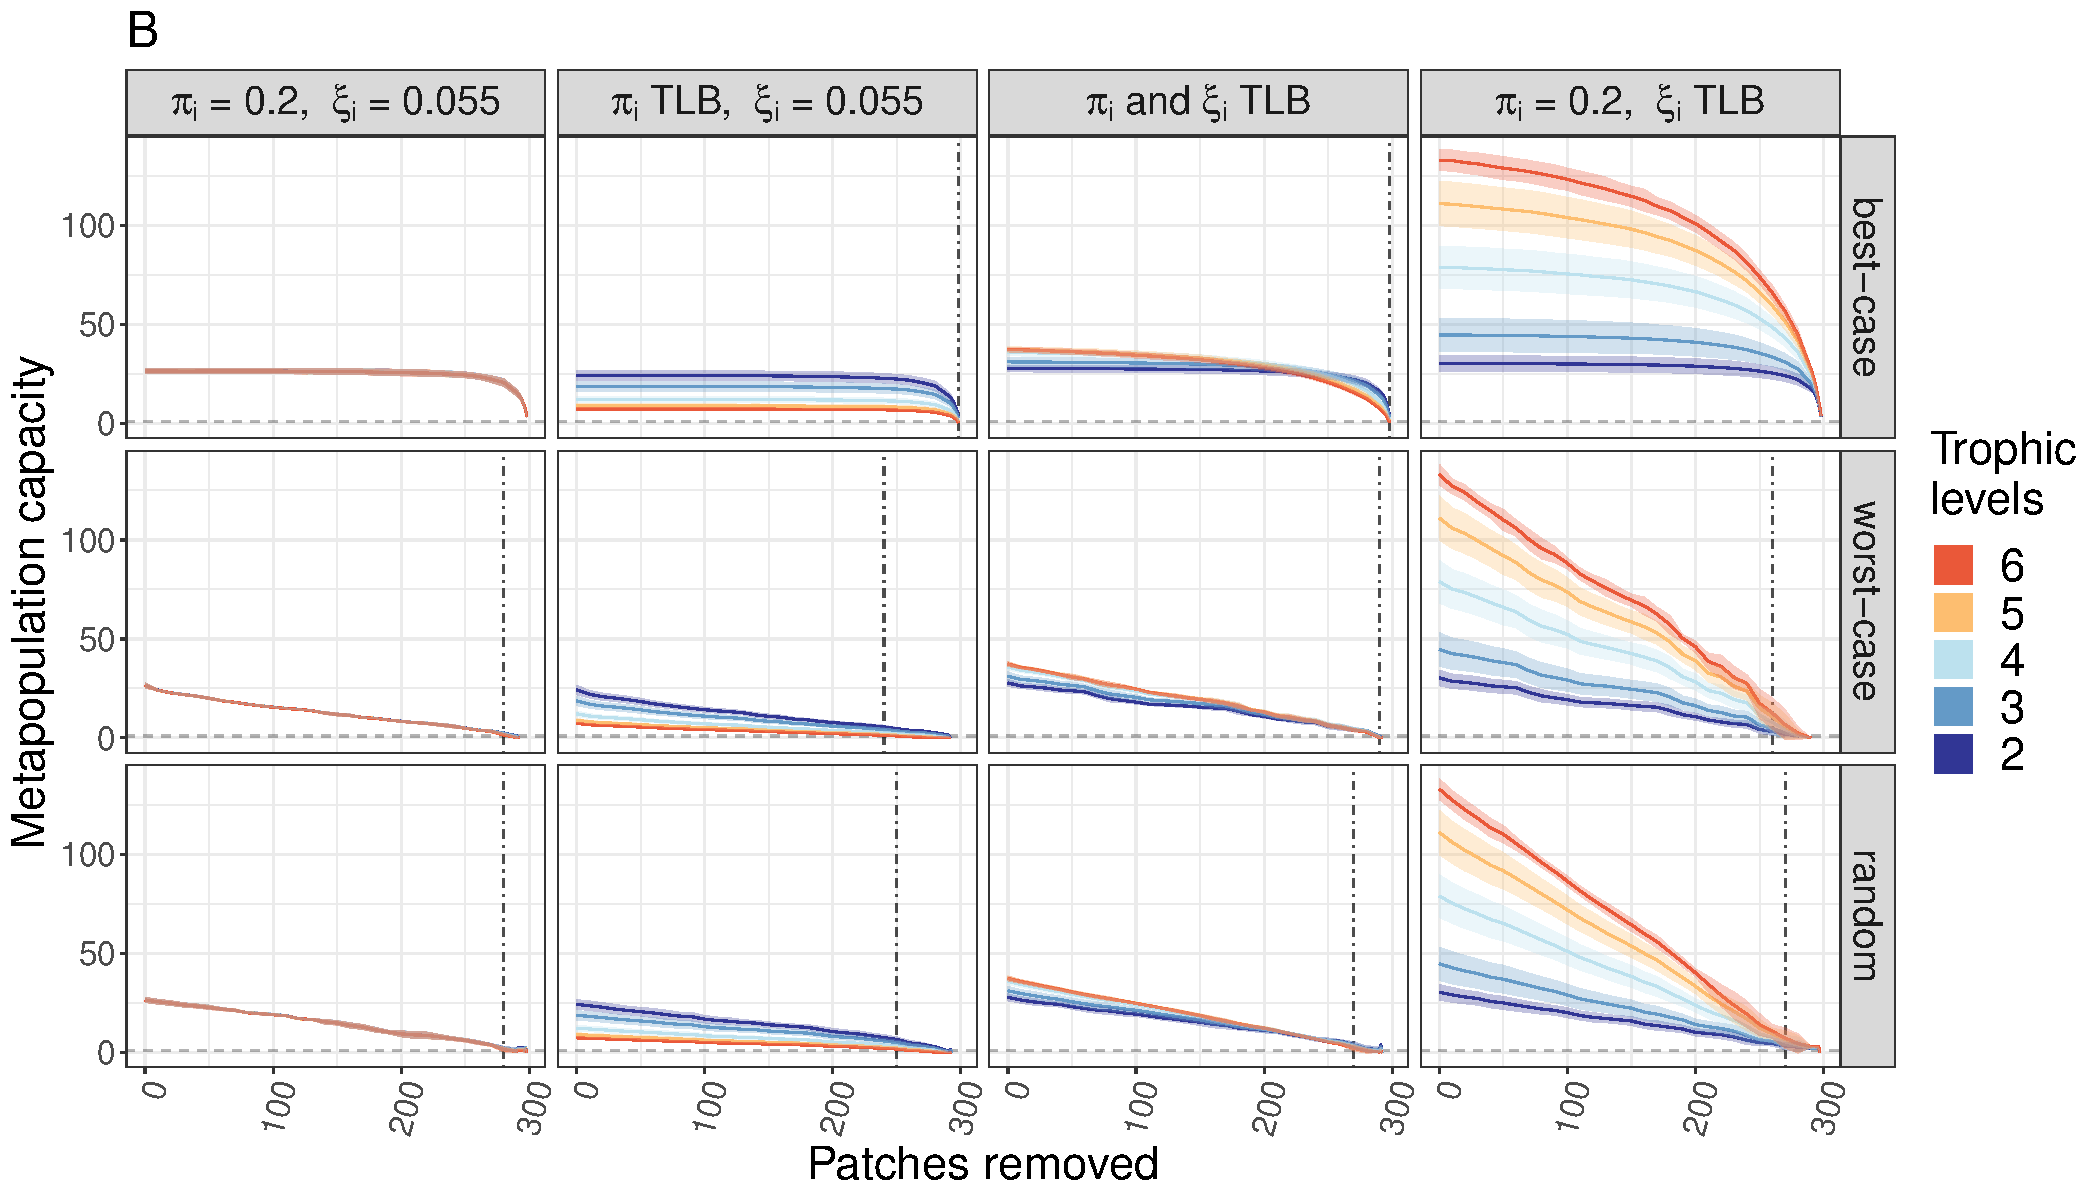
\includegraphics[width=0.8\textwidth,valign=t]{lambda_Model_food_web_with_200_consumer_and_200_basal_species_basal_5_1.pdf}
    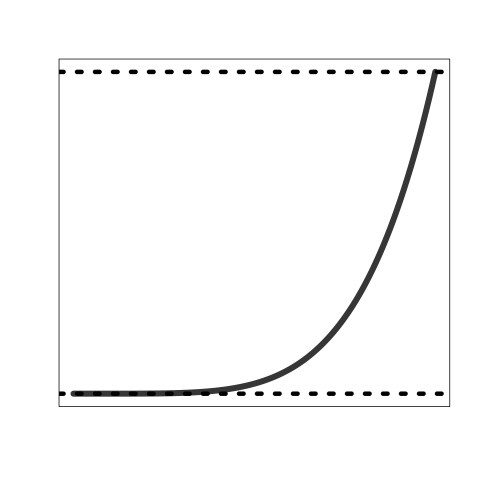
\includegraphics[width=0.19\textwidth,valign=t]{fform_5_1.png}
 \caption{As Figure \ref{S_fig:patchloss_350_50_1}, but with 200 consumer and 200 basal species.}
 \label{S_fig:patchloss_200_200_1}
\end{figure}

\begin{figure}\ContinuedFloat
 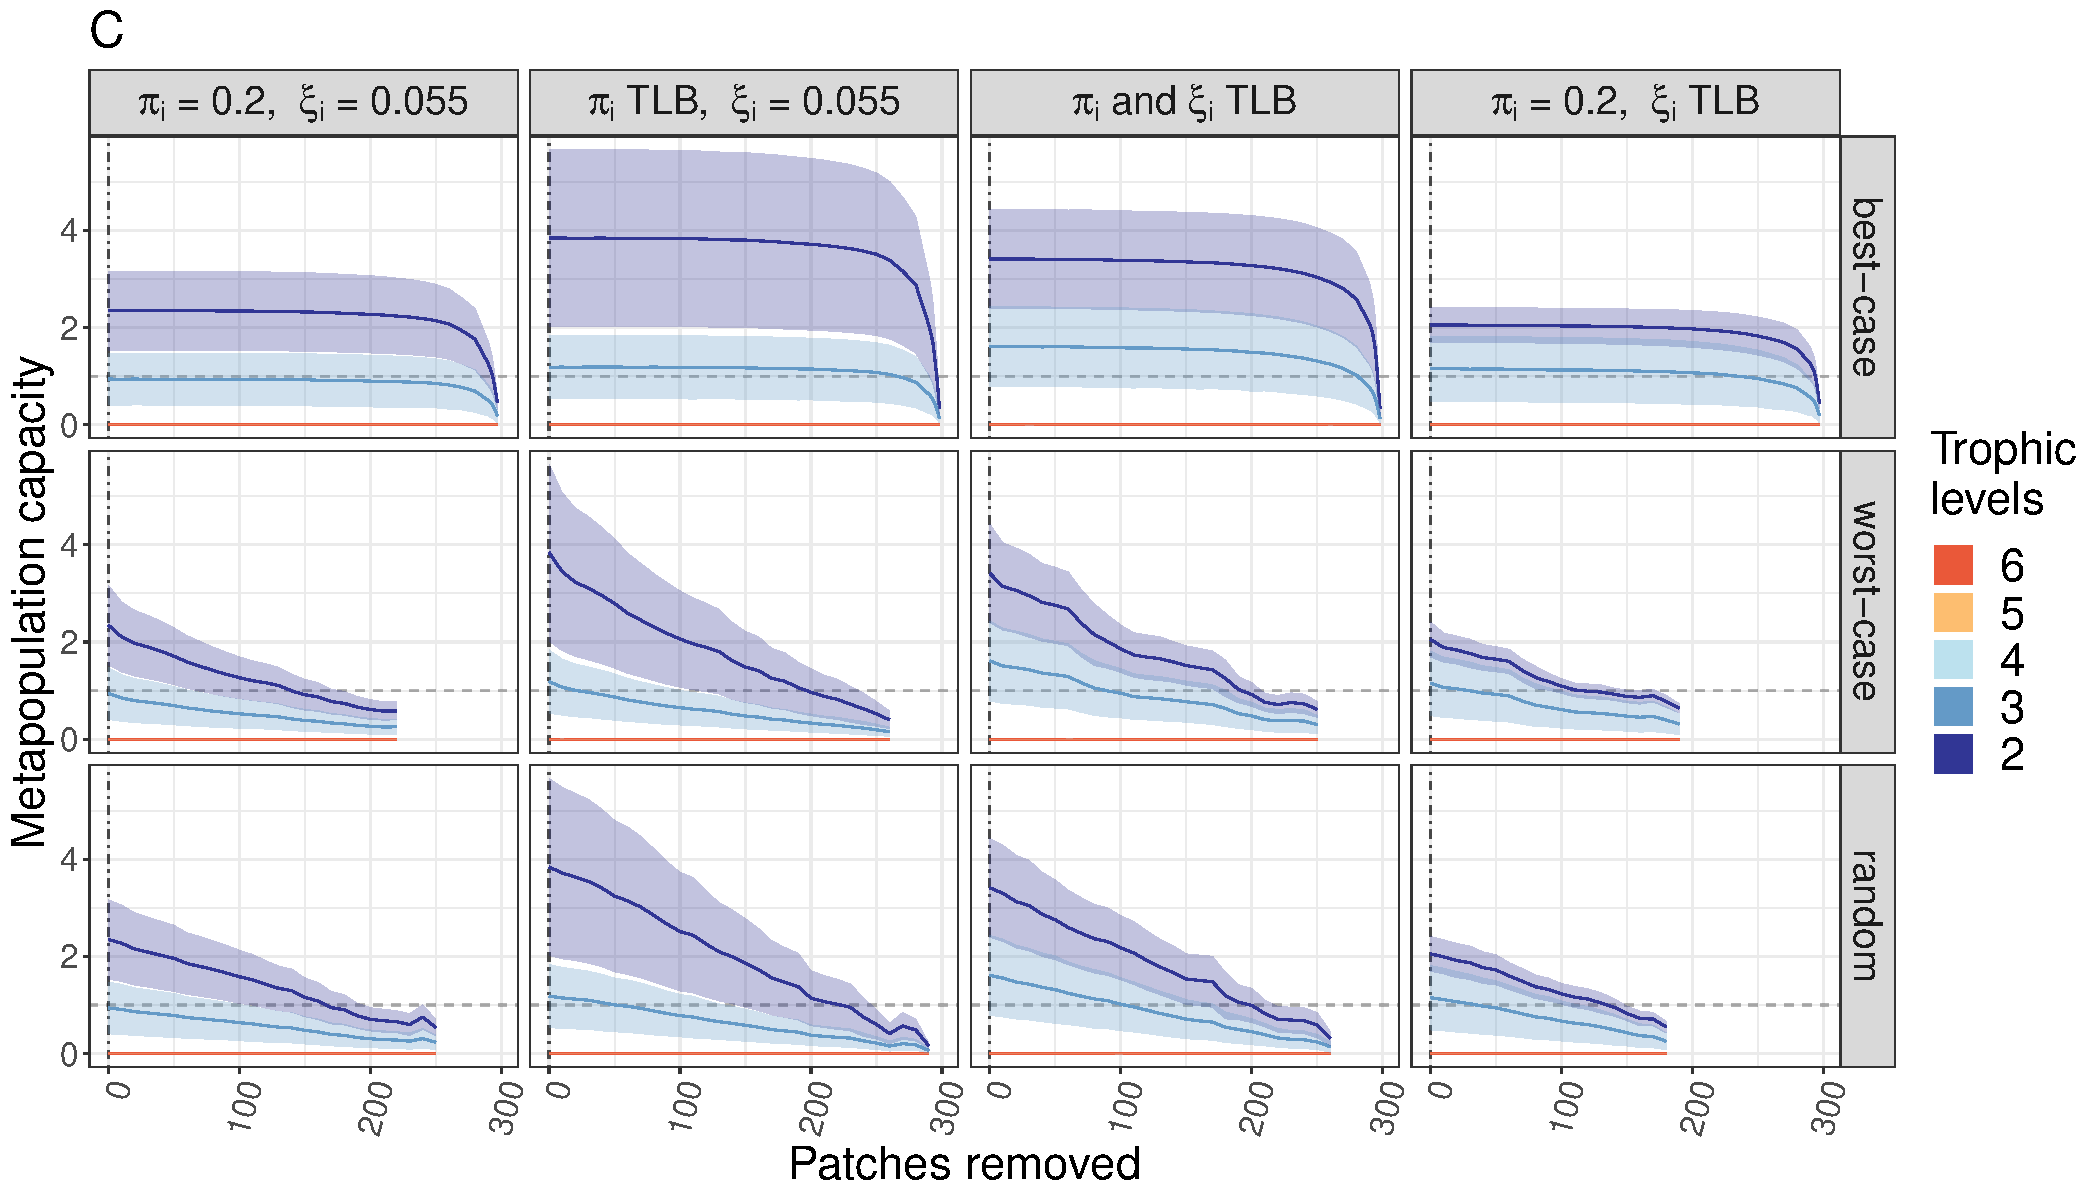
\includegraphics[width=0.8\textwidth,valign=t]{lambda_Model_food_web_with_200_consumer_and_200_basal_species_basal_1_5.pdf}
  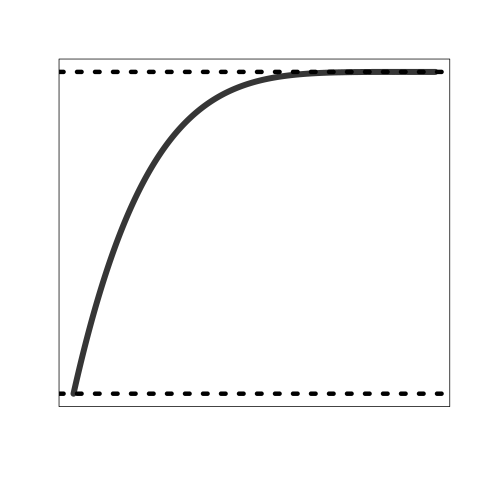
\includegraphics[width=0.19\textwidth,valign=t]{fform_1_5.png}
  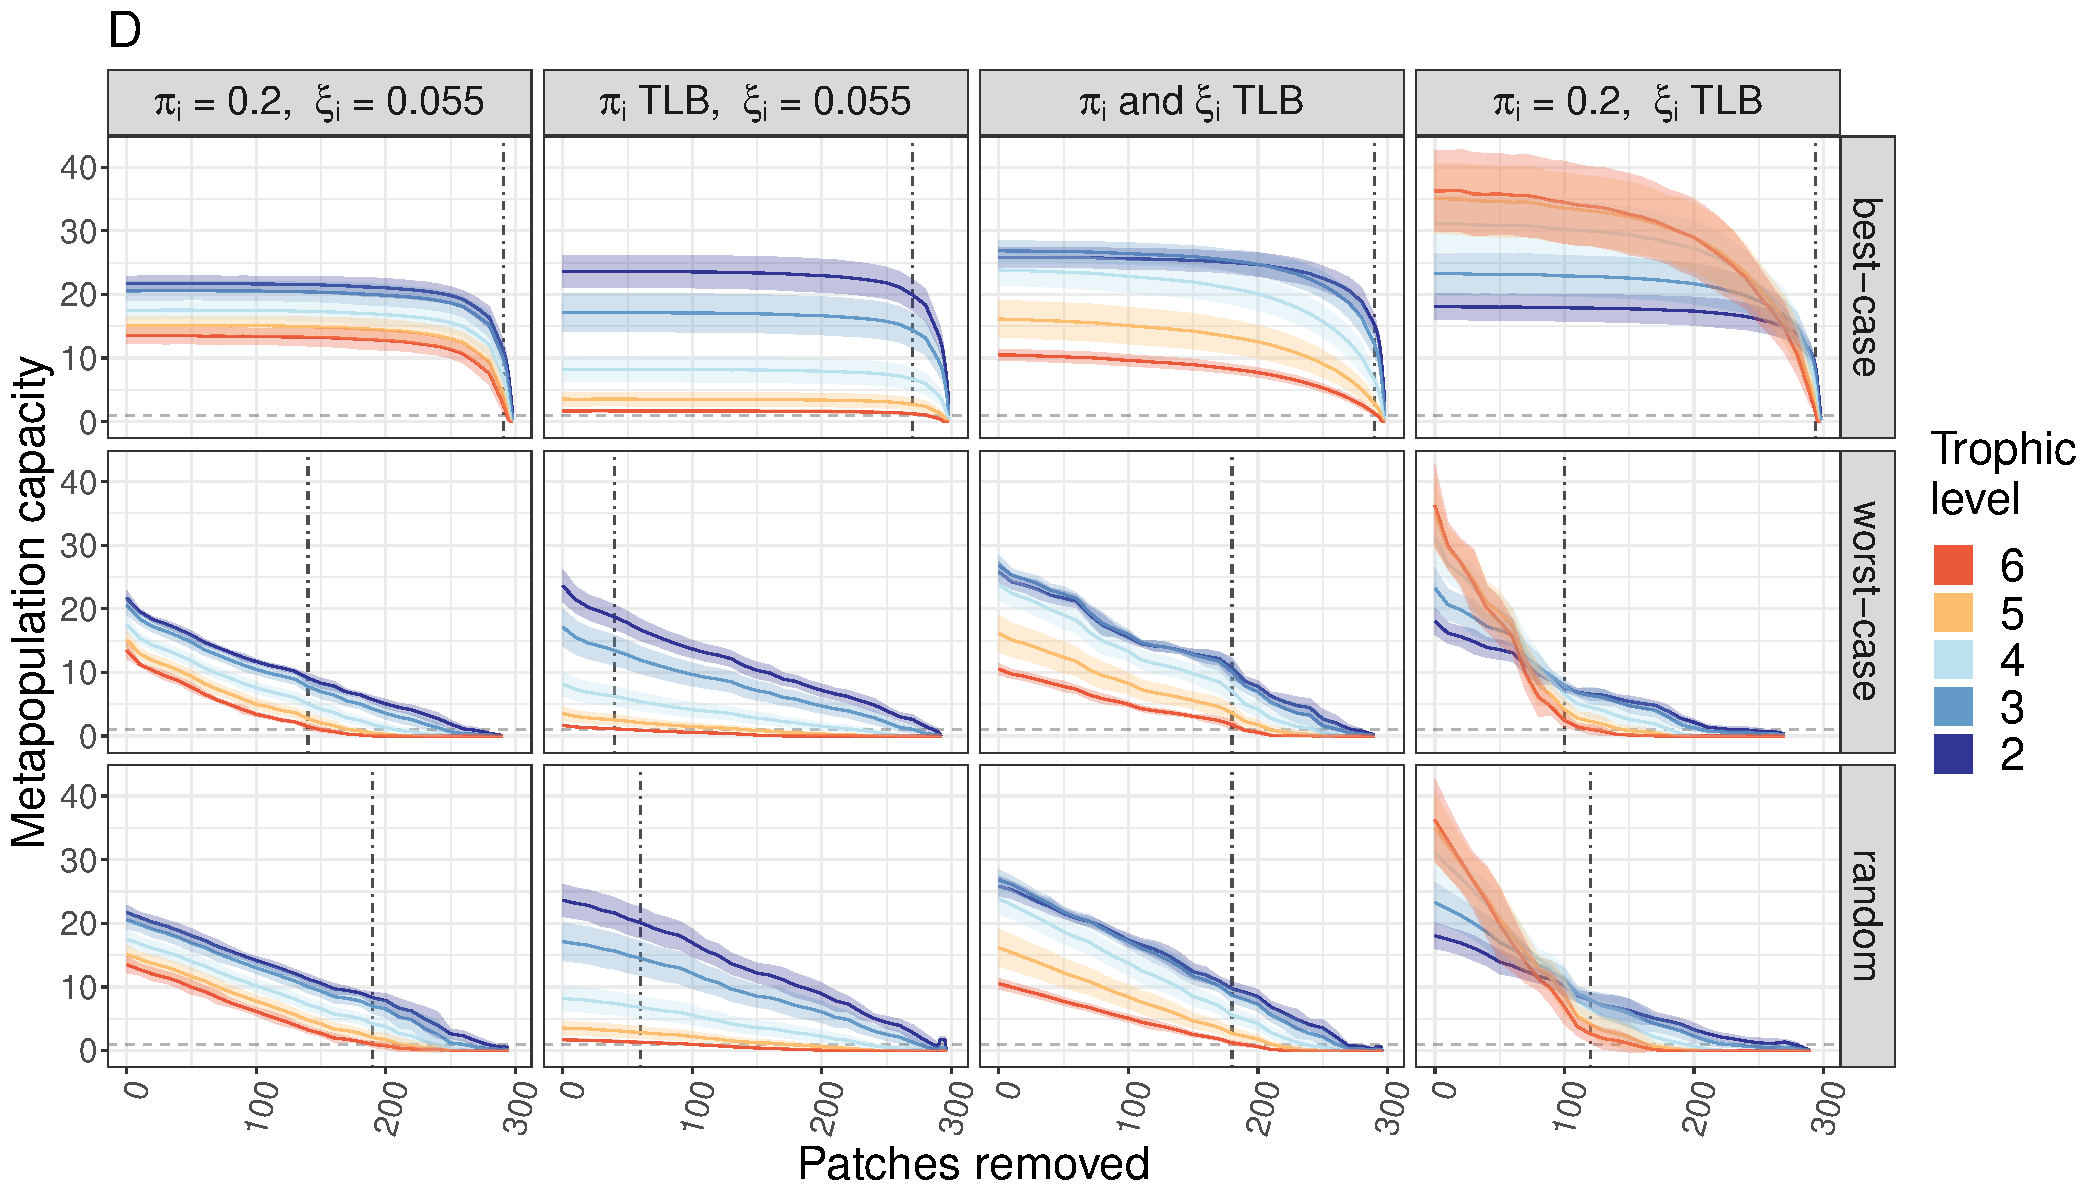
\includegraphics[width=0.8\textwidth,valign=t]{lambda_Model_food_web_with_200_consumer_and_200_basal_species_basal_5_5.pdf}
  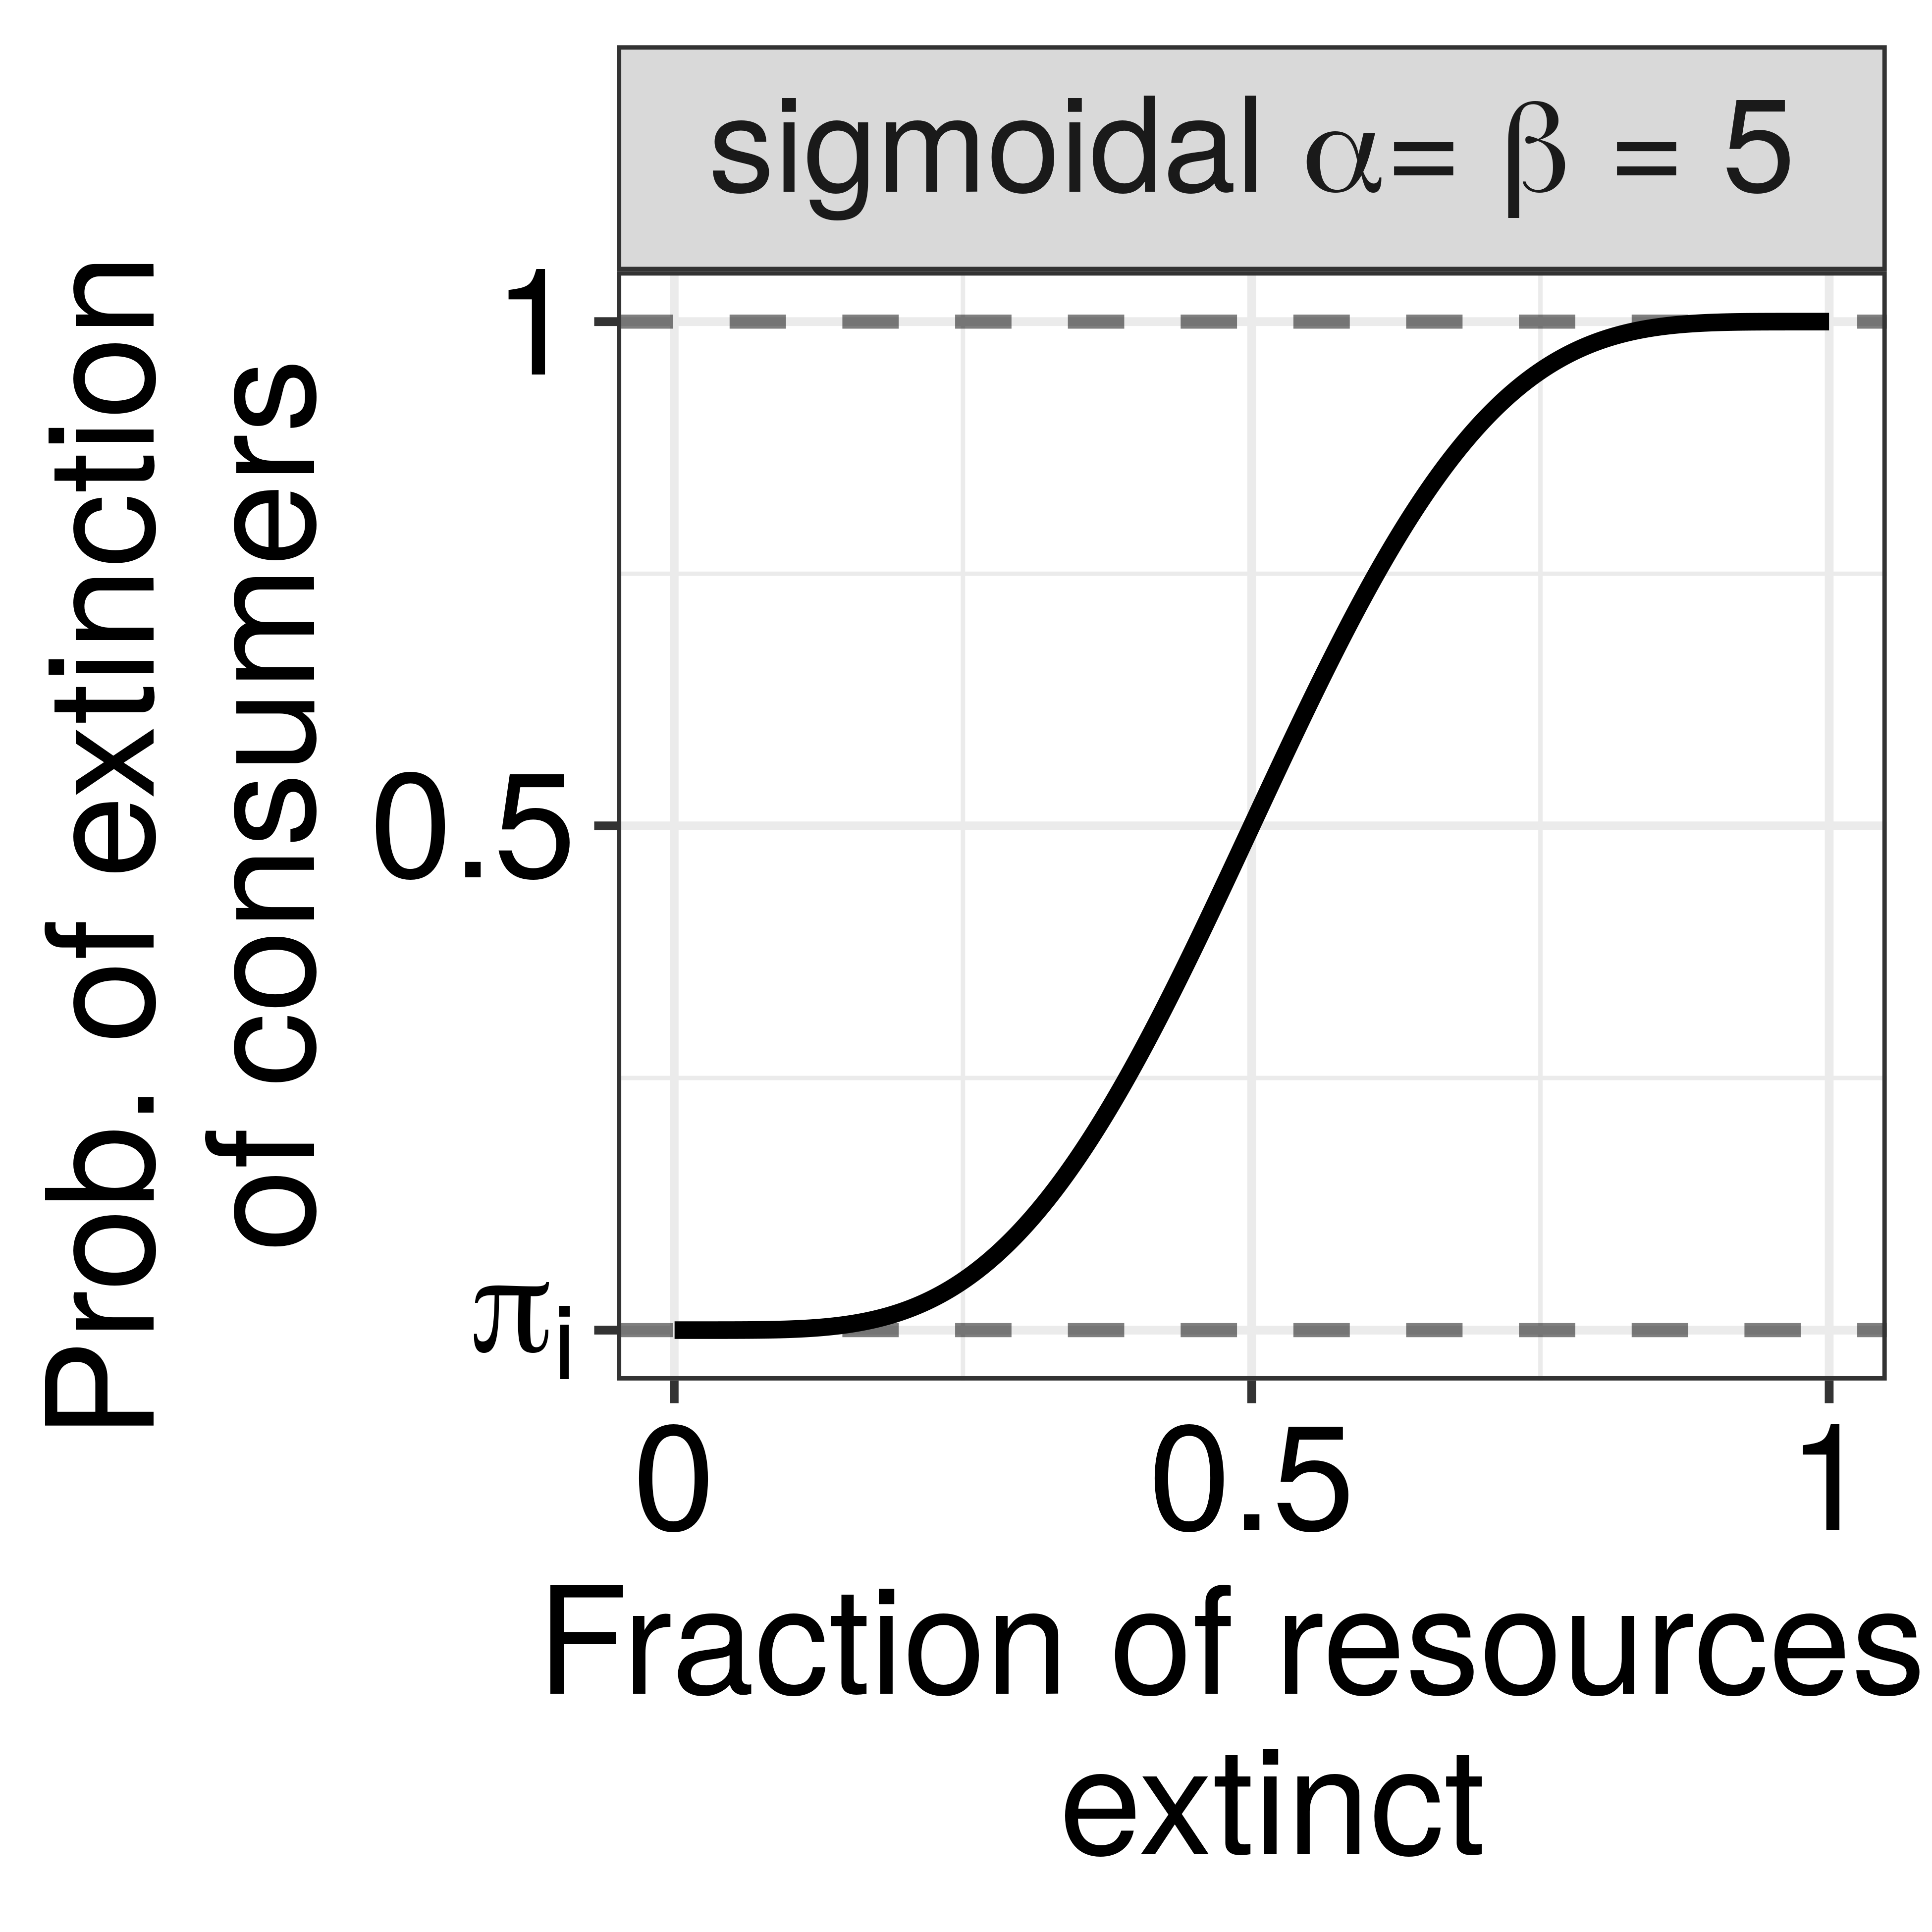
\includegraphics[width=0.19\textwidth,valign=t]{fform_5_5.png}
 \caption{Figure continued.}
 \label{S_fig:patchloss_200_200_2}
\end{figure}

\begin{figure}
  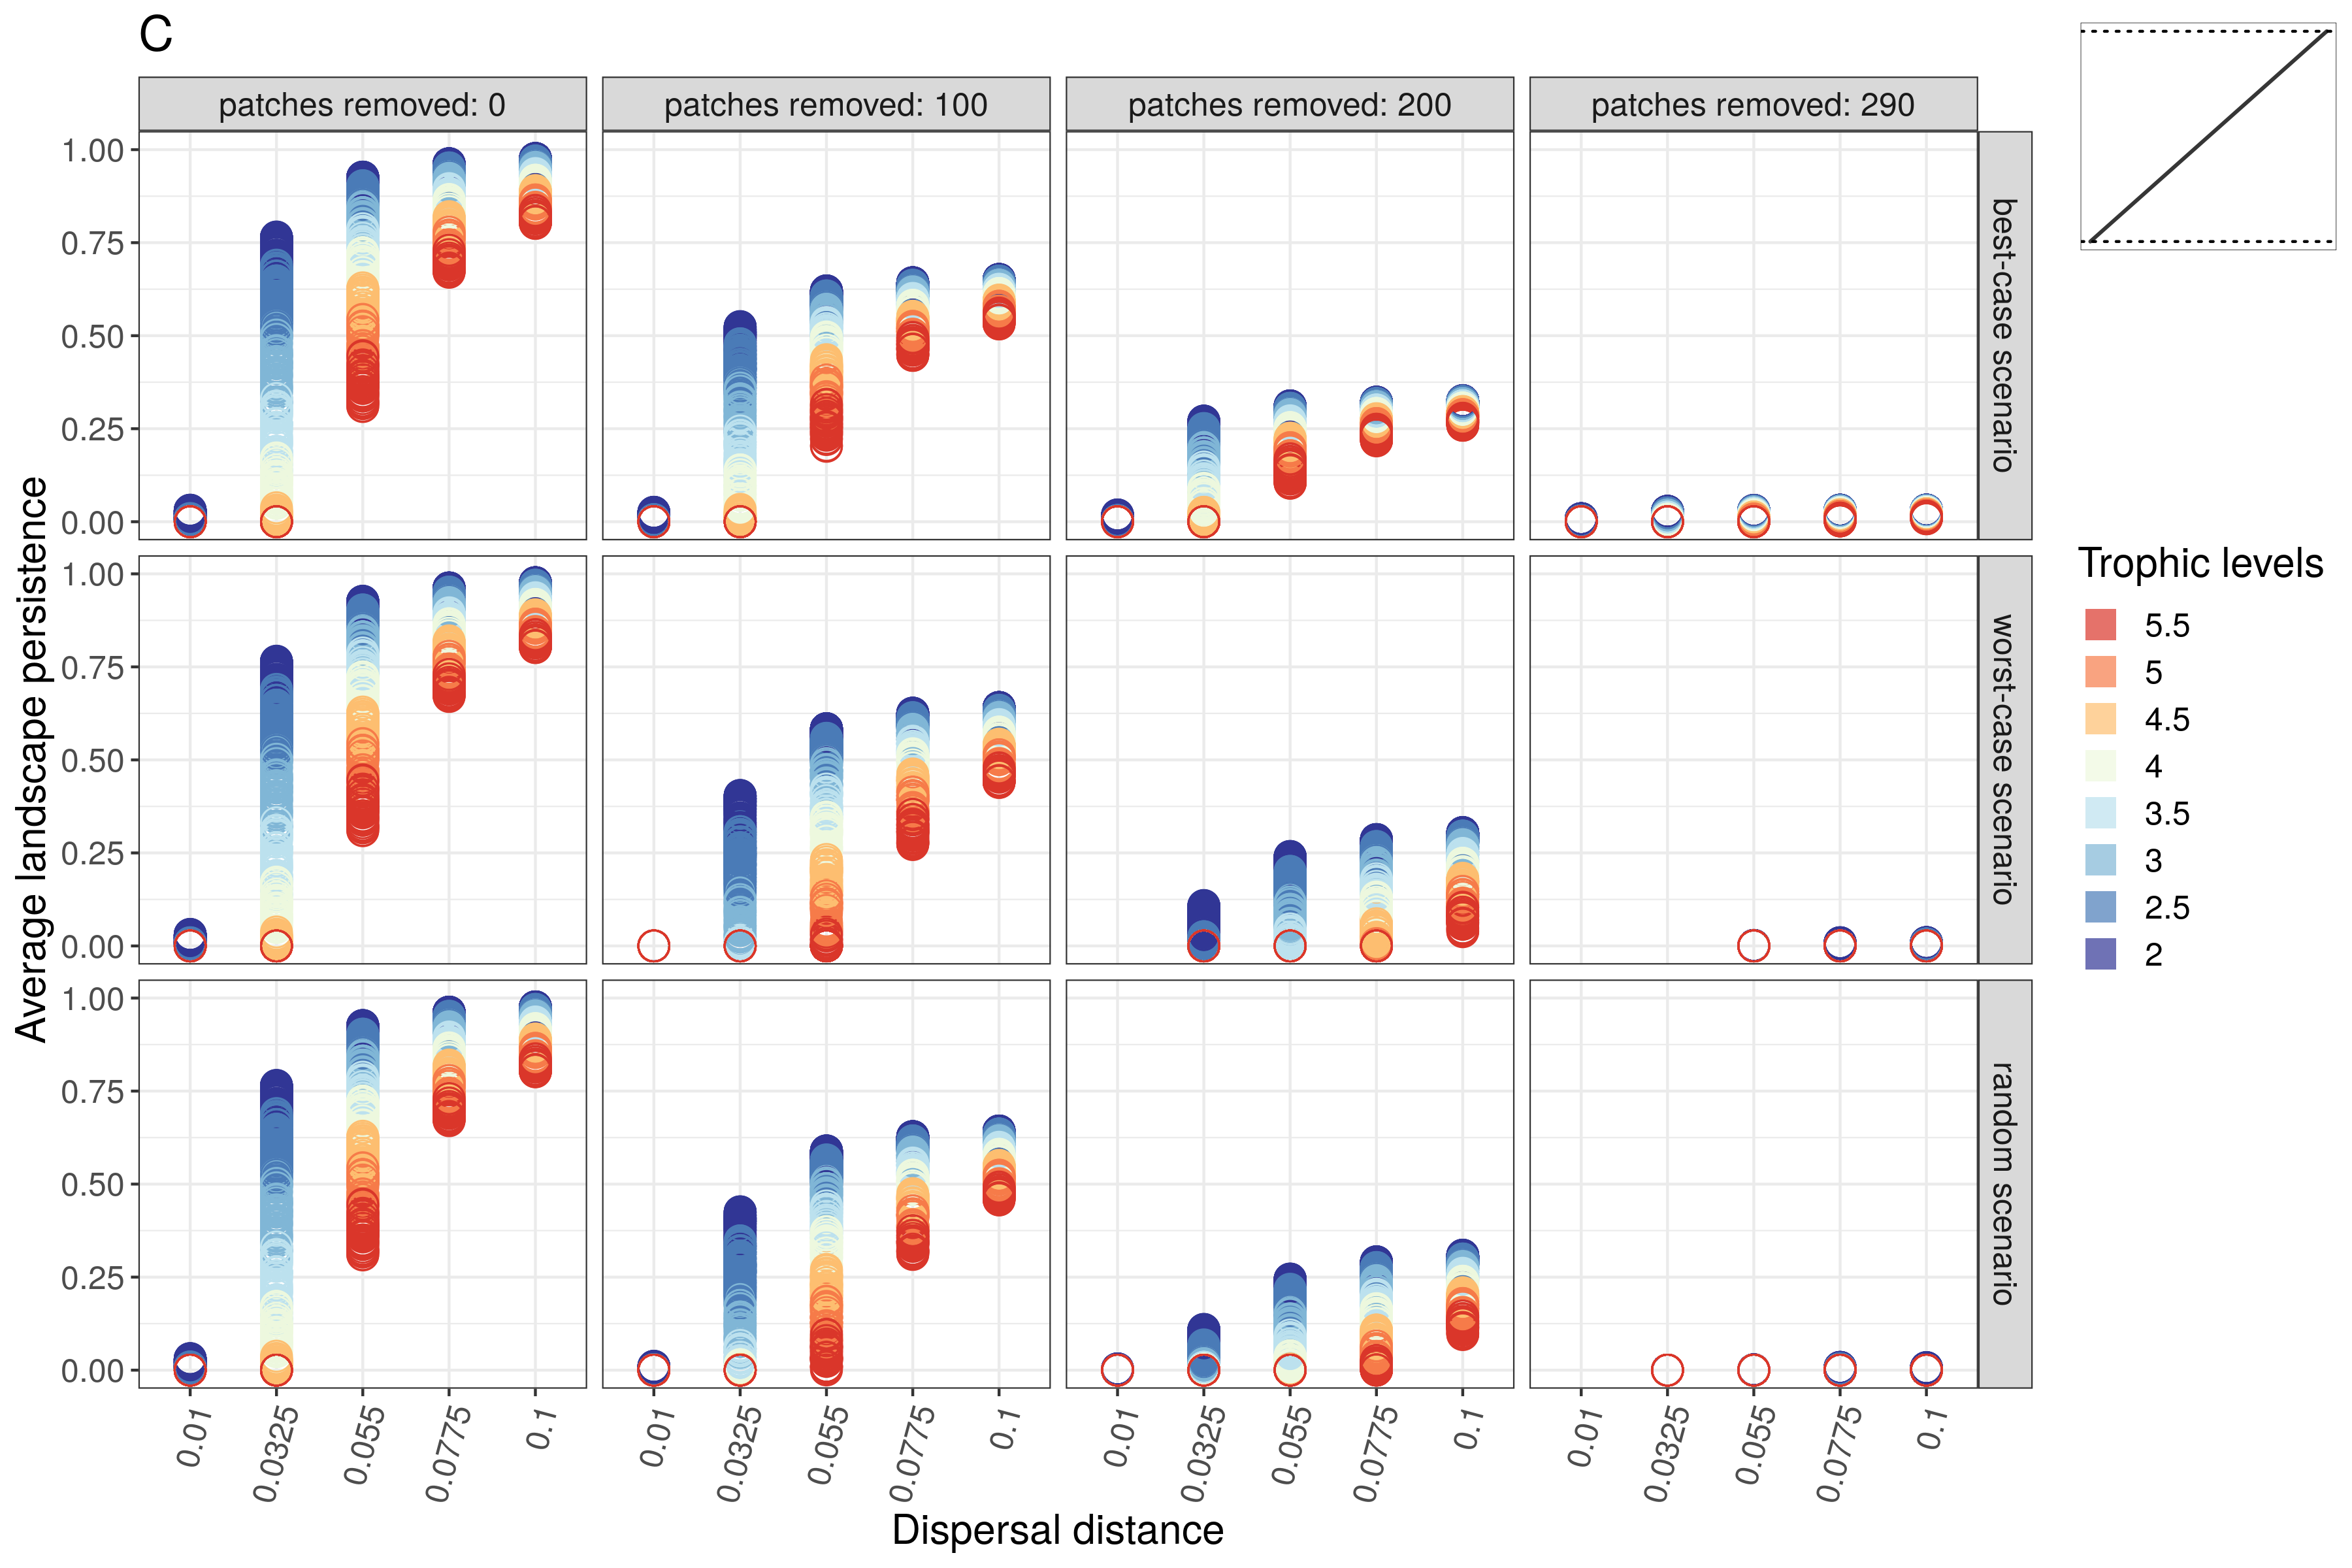
\includegraphics[width=0.8\textwidth,valign=t]{sump_Model_food_web_with_200_consumer_and_200_basal_species_basal_1_1.png}
  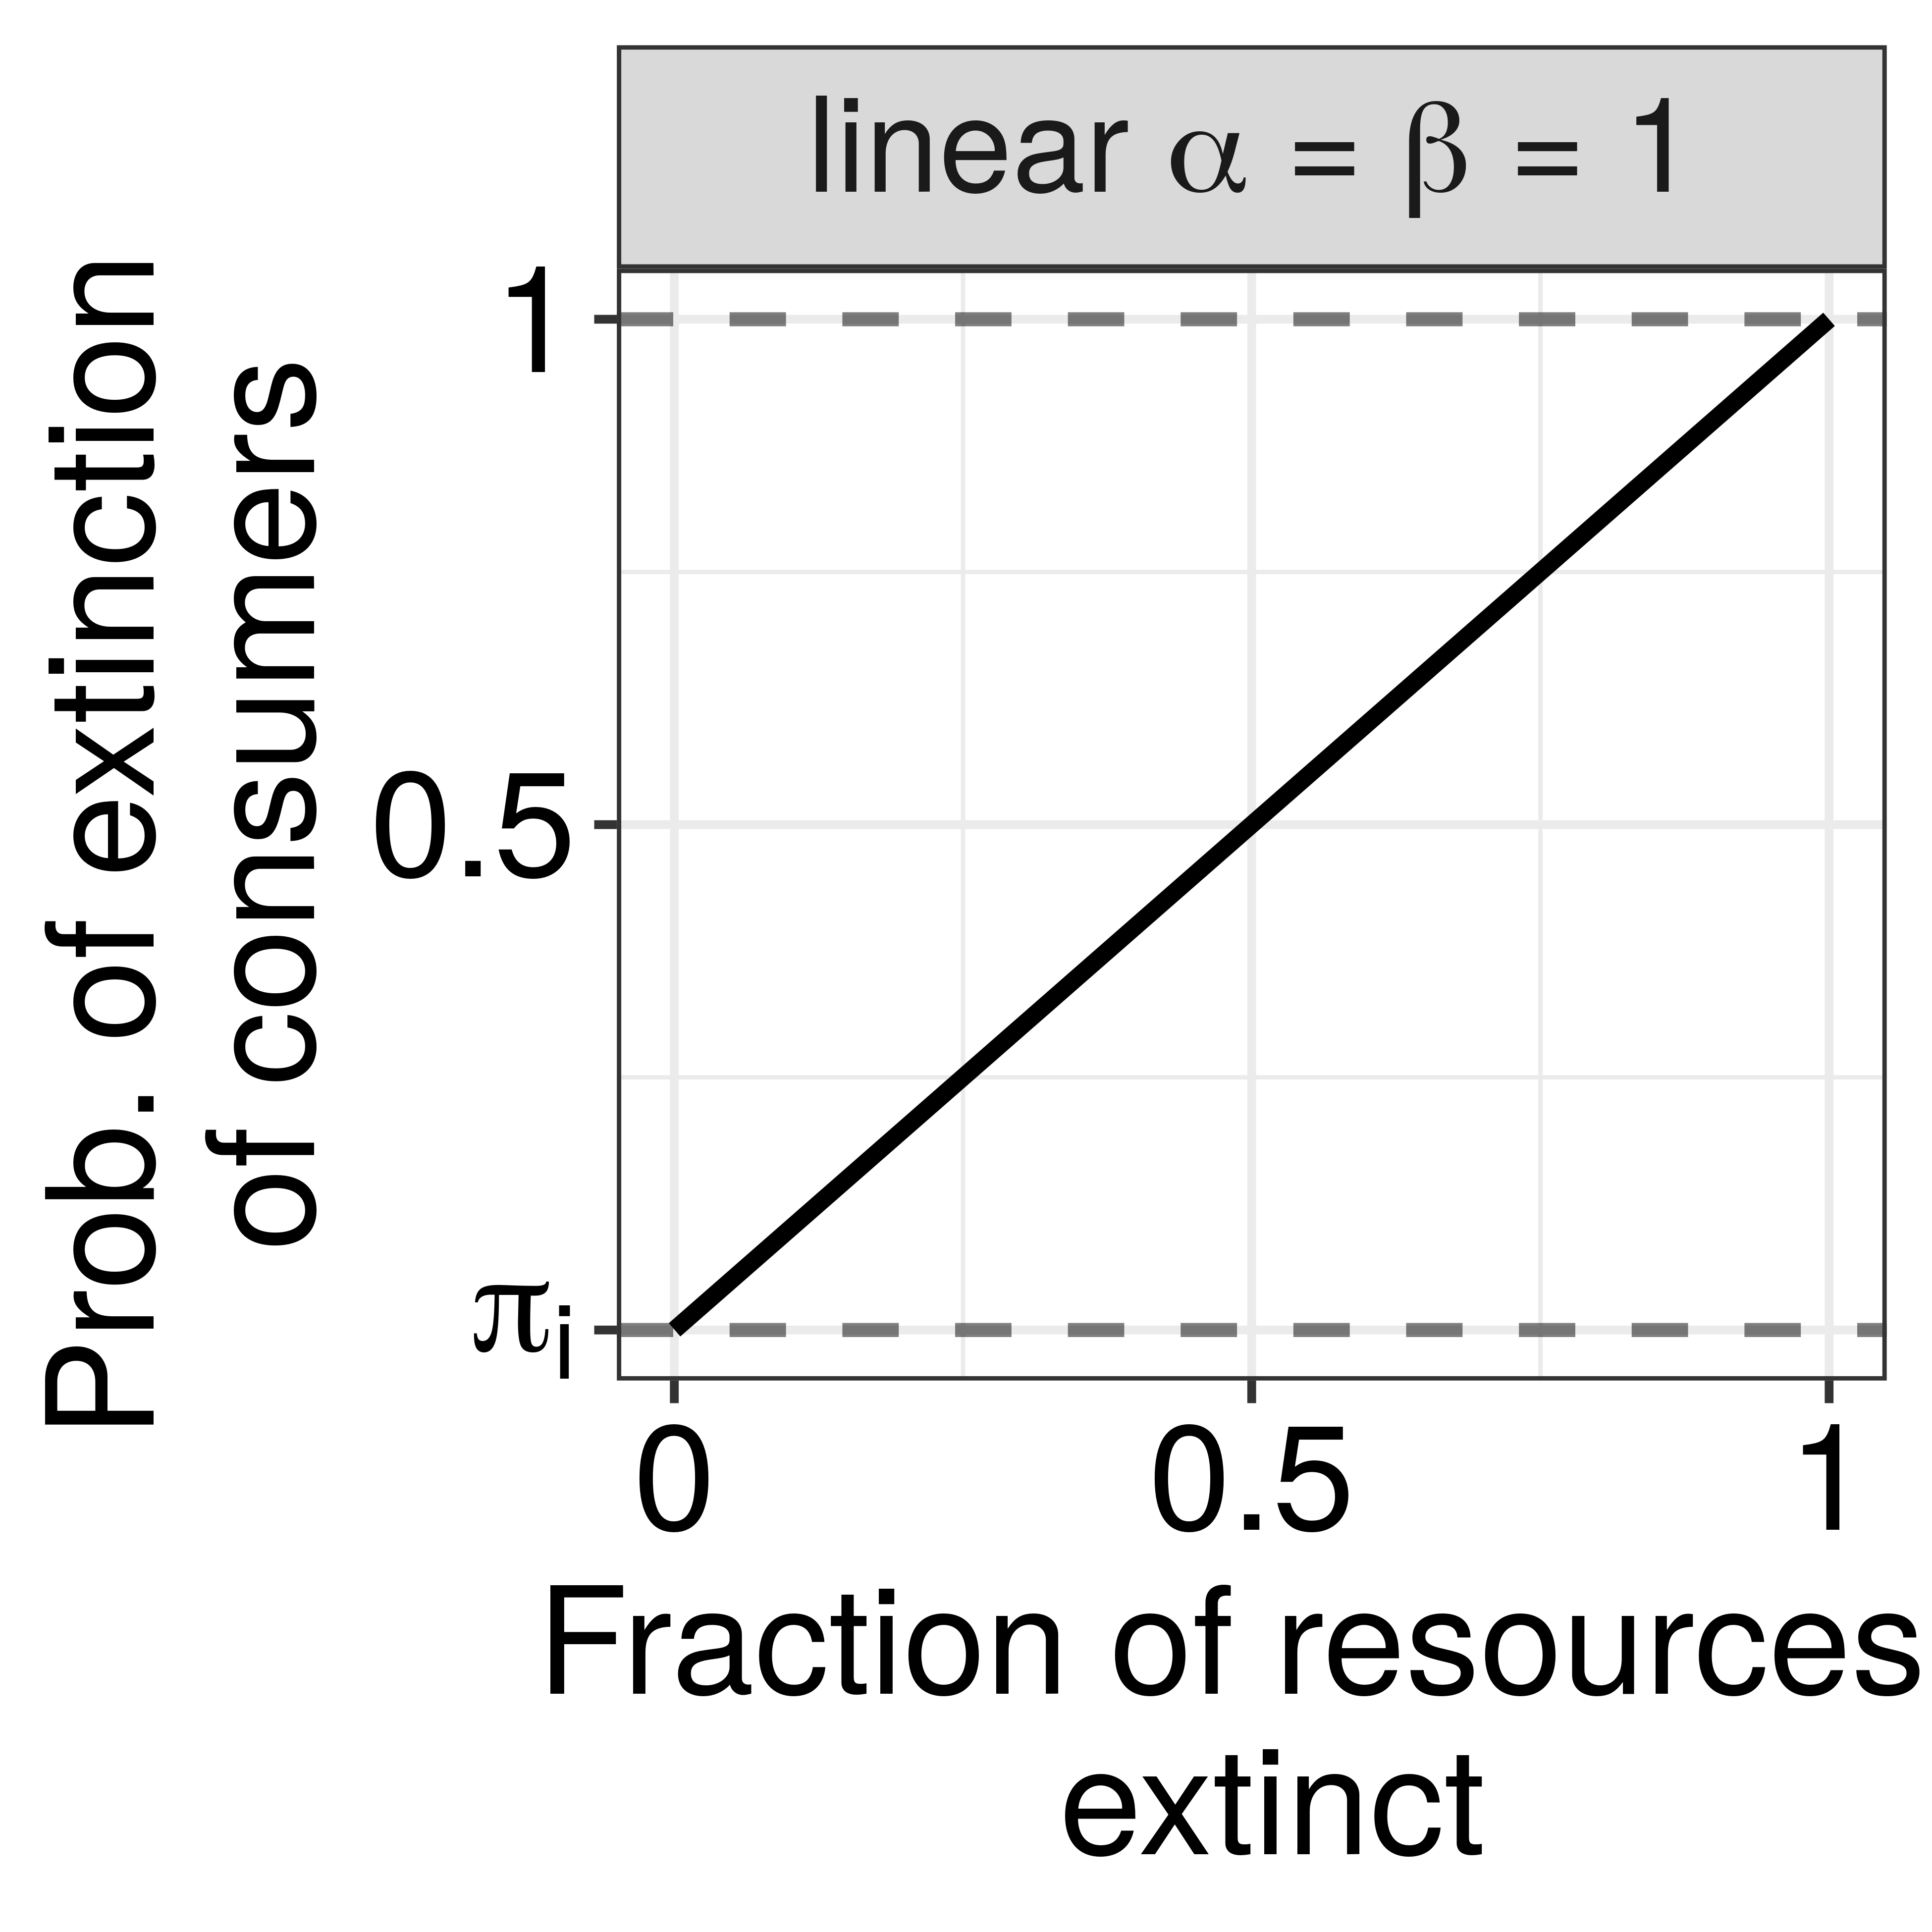
\includegraphics[width=0.19\textwidth,valign=t]{fform_1_1.png}
  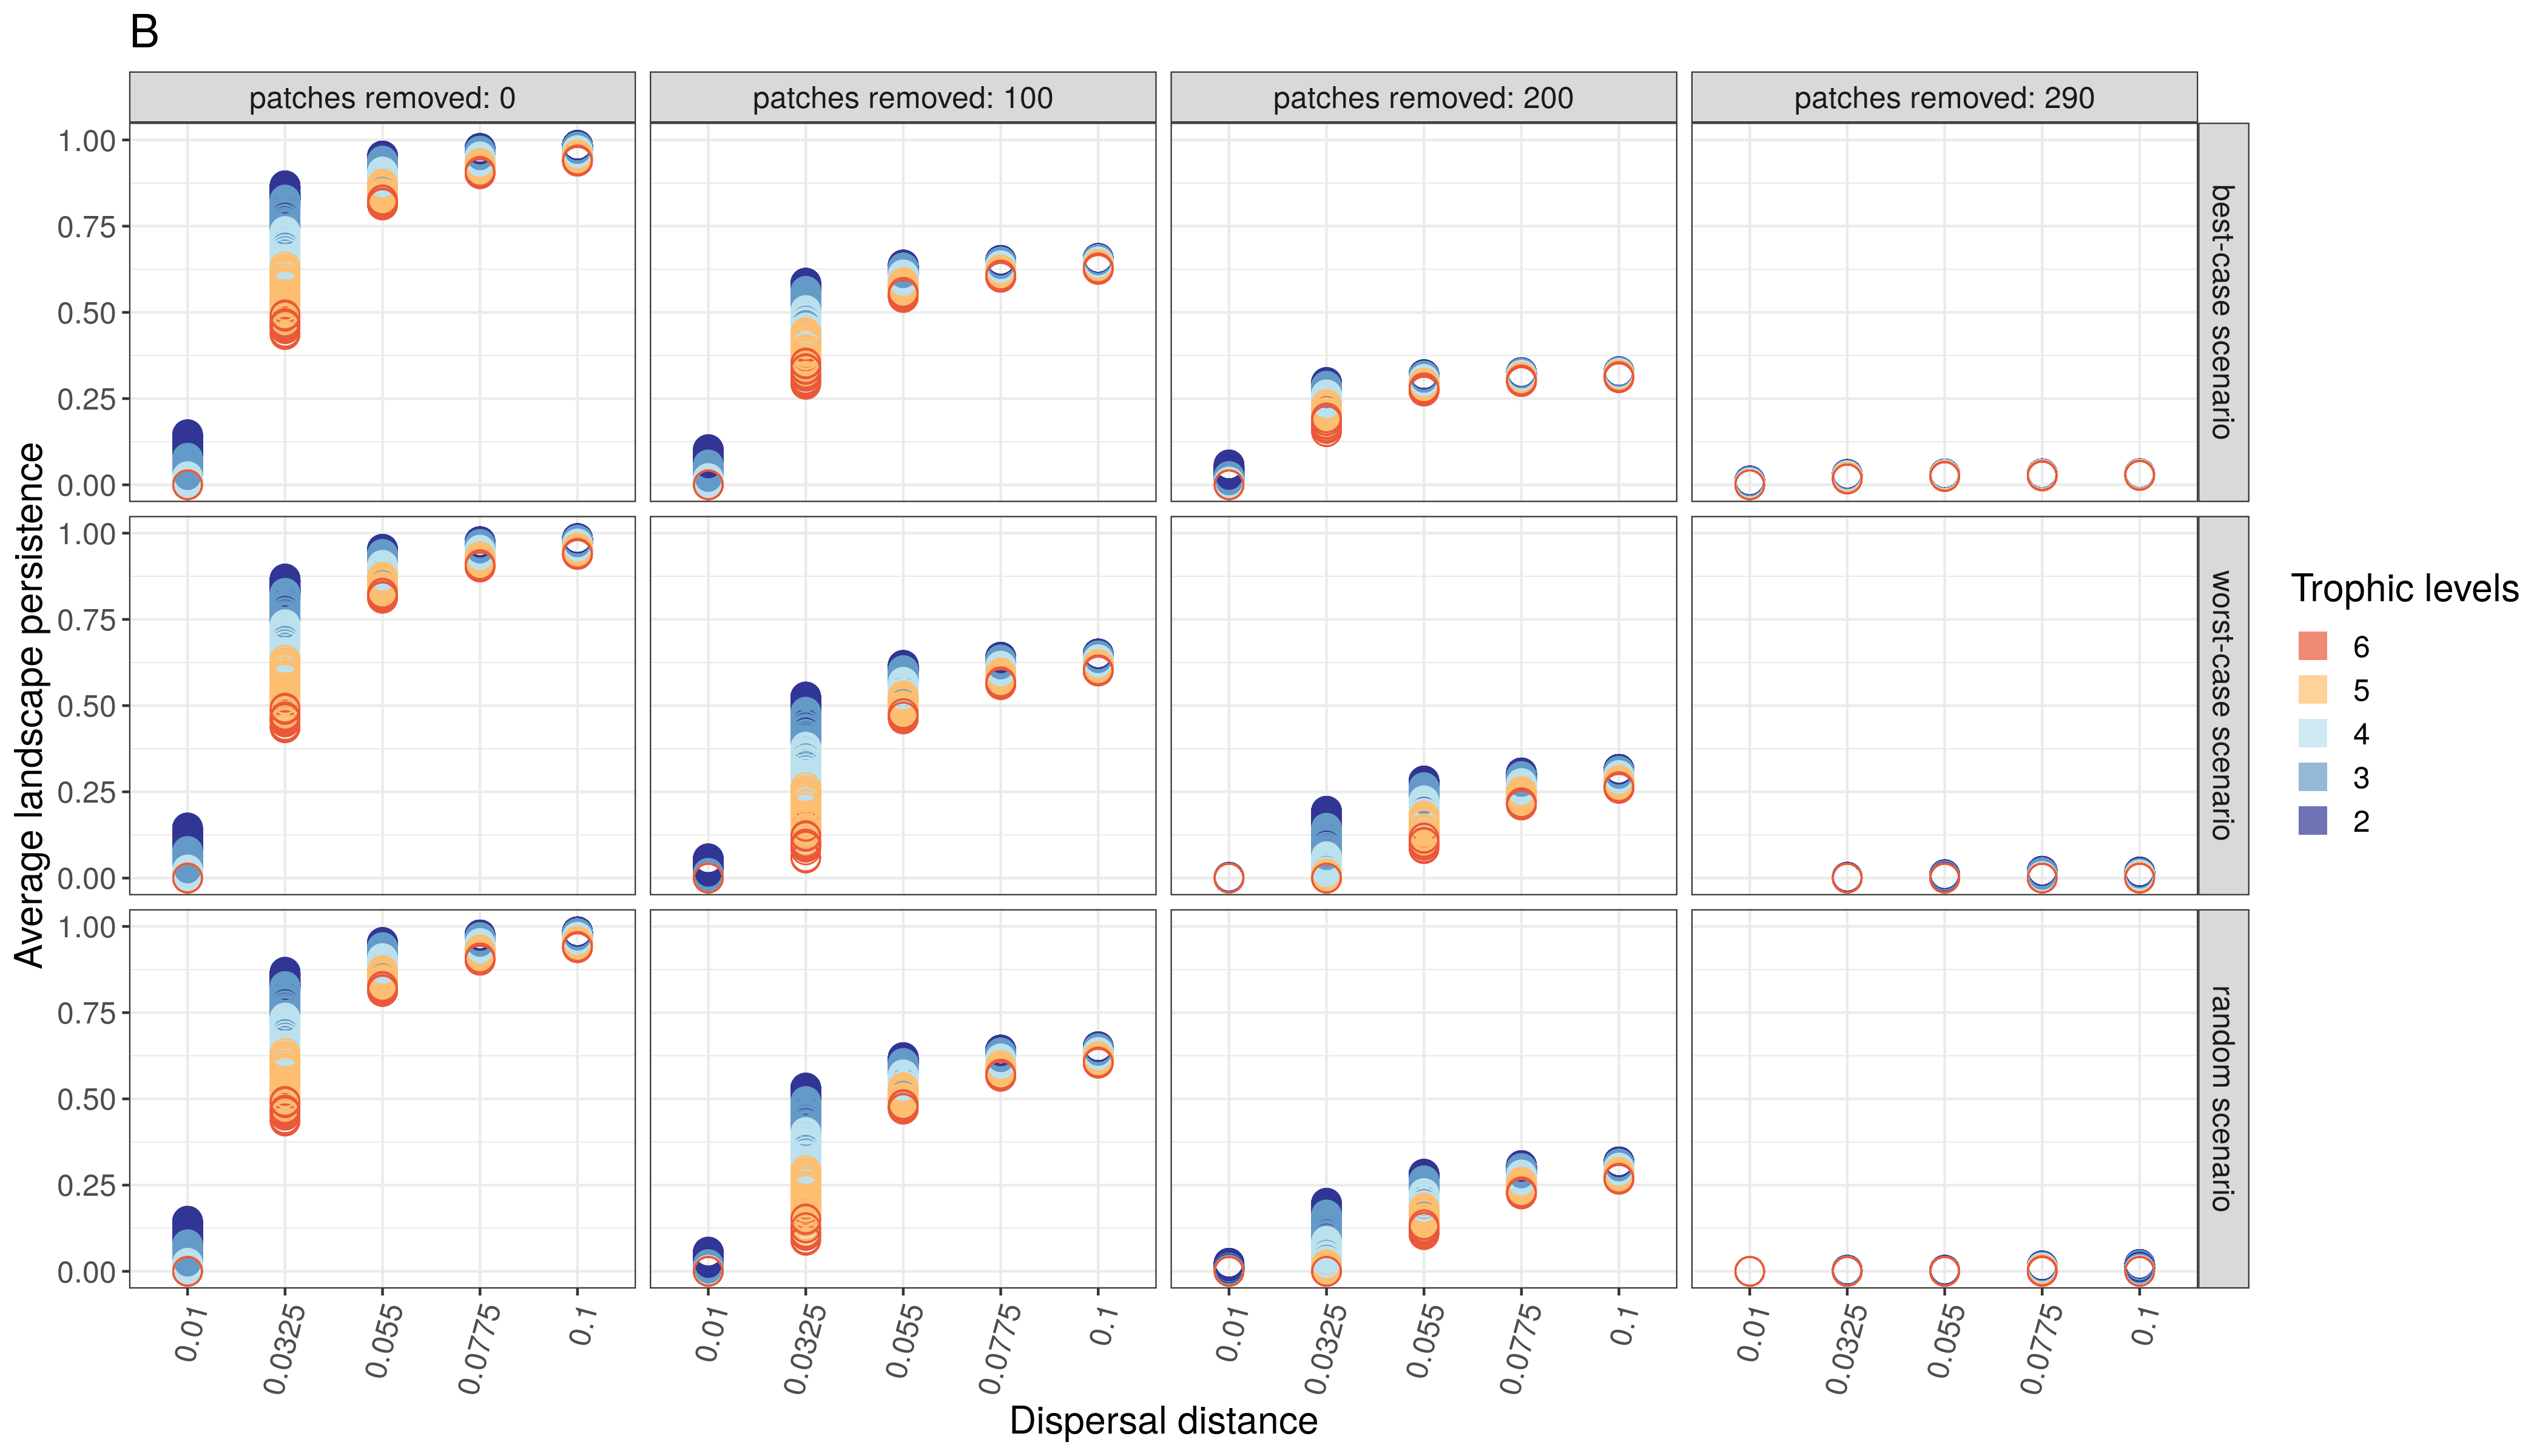
\includegraphics[width=0.8\textwidth,valign=t]{sump_Model_food_web_with_200_consumer_and_200_basal_species_basal_5_1.png}
    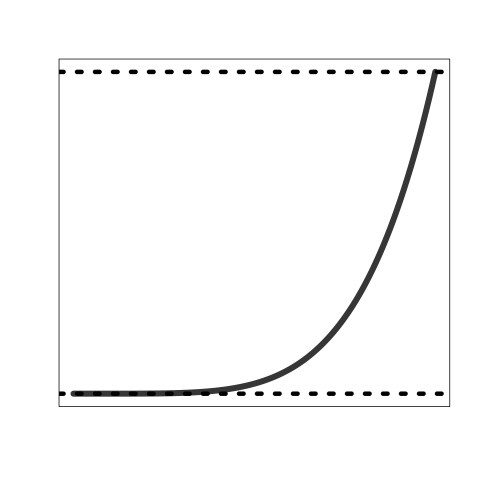
\includegraphics[width=0.19\textwidth,valign=t]{fform_5_1.png}
 \caption{As Figure \ref{S_fig:patchloss_300_100_distance_1}, but with 200 consumer and 200 basal species.}
   \label{S_fig:patchloss_200_200_distance_1}
\end{figure}

\begin{figure}\ContinuedFloat
  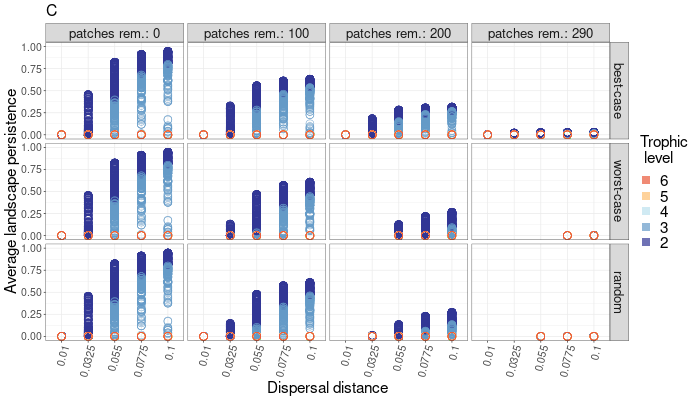
\includegraphics[width=0.8\textwidth,valign=t]{sump_Model_food_web_with_200_consumer_and_200_basal_species_basal_1_5.png}
  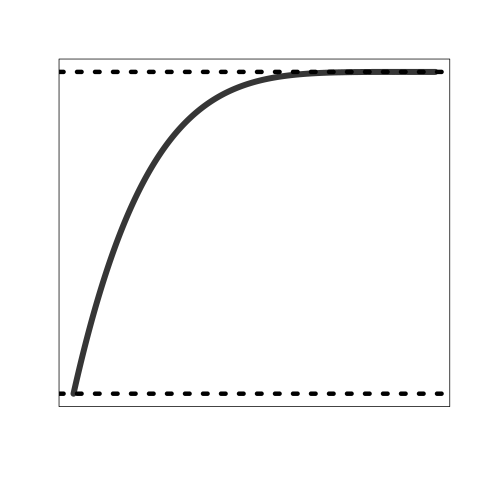
\includegraphics[width=0.19\textwidth,valign=t]{fform_1_5.png}
  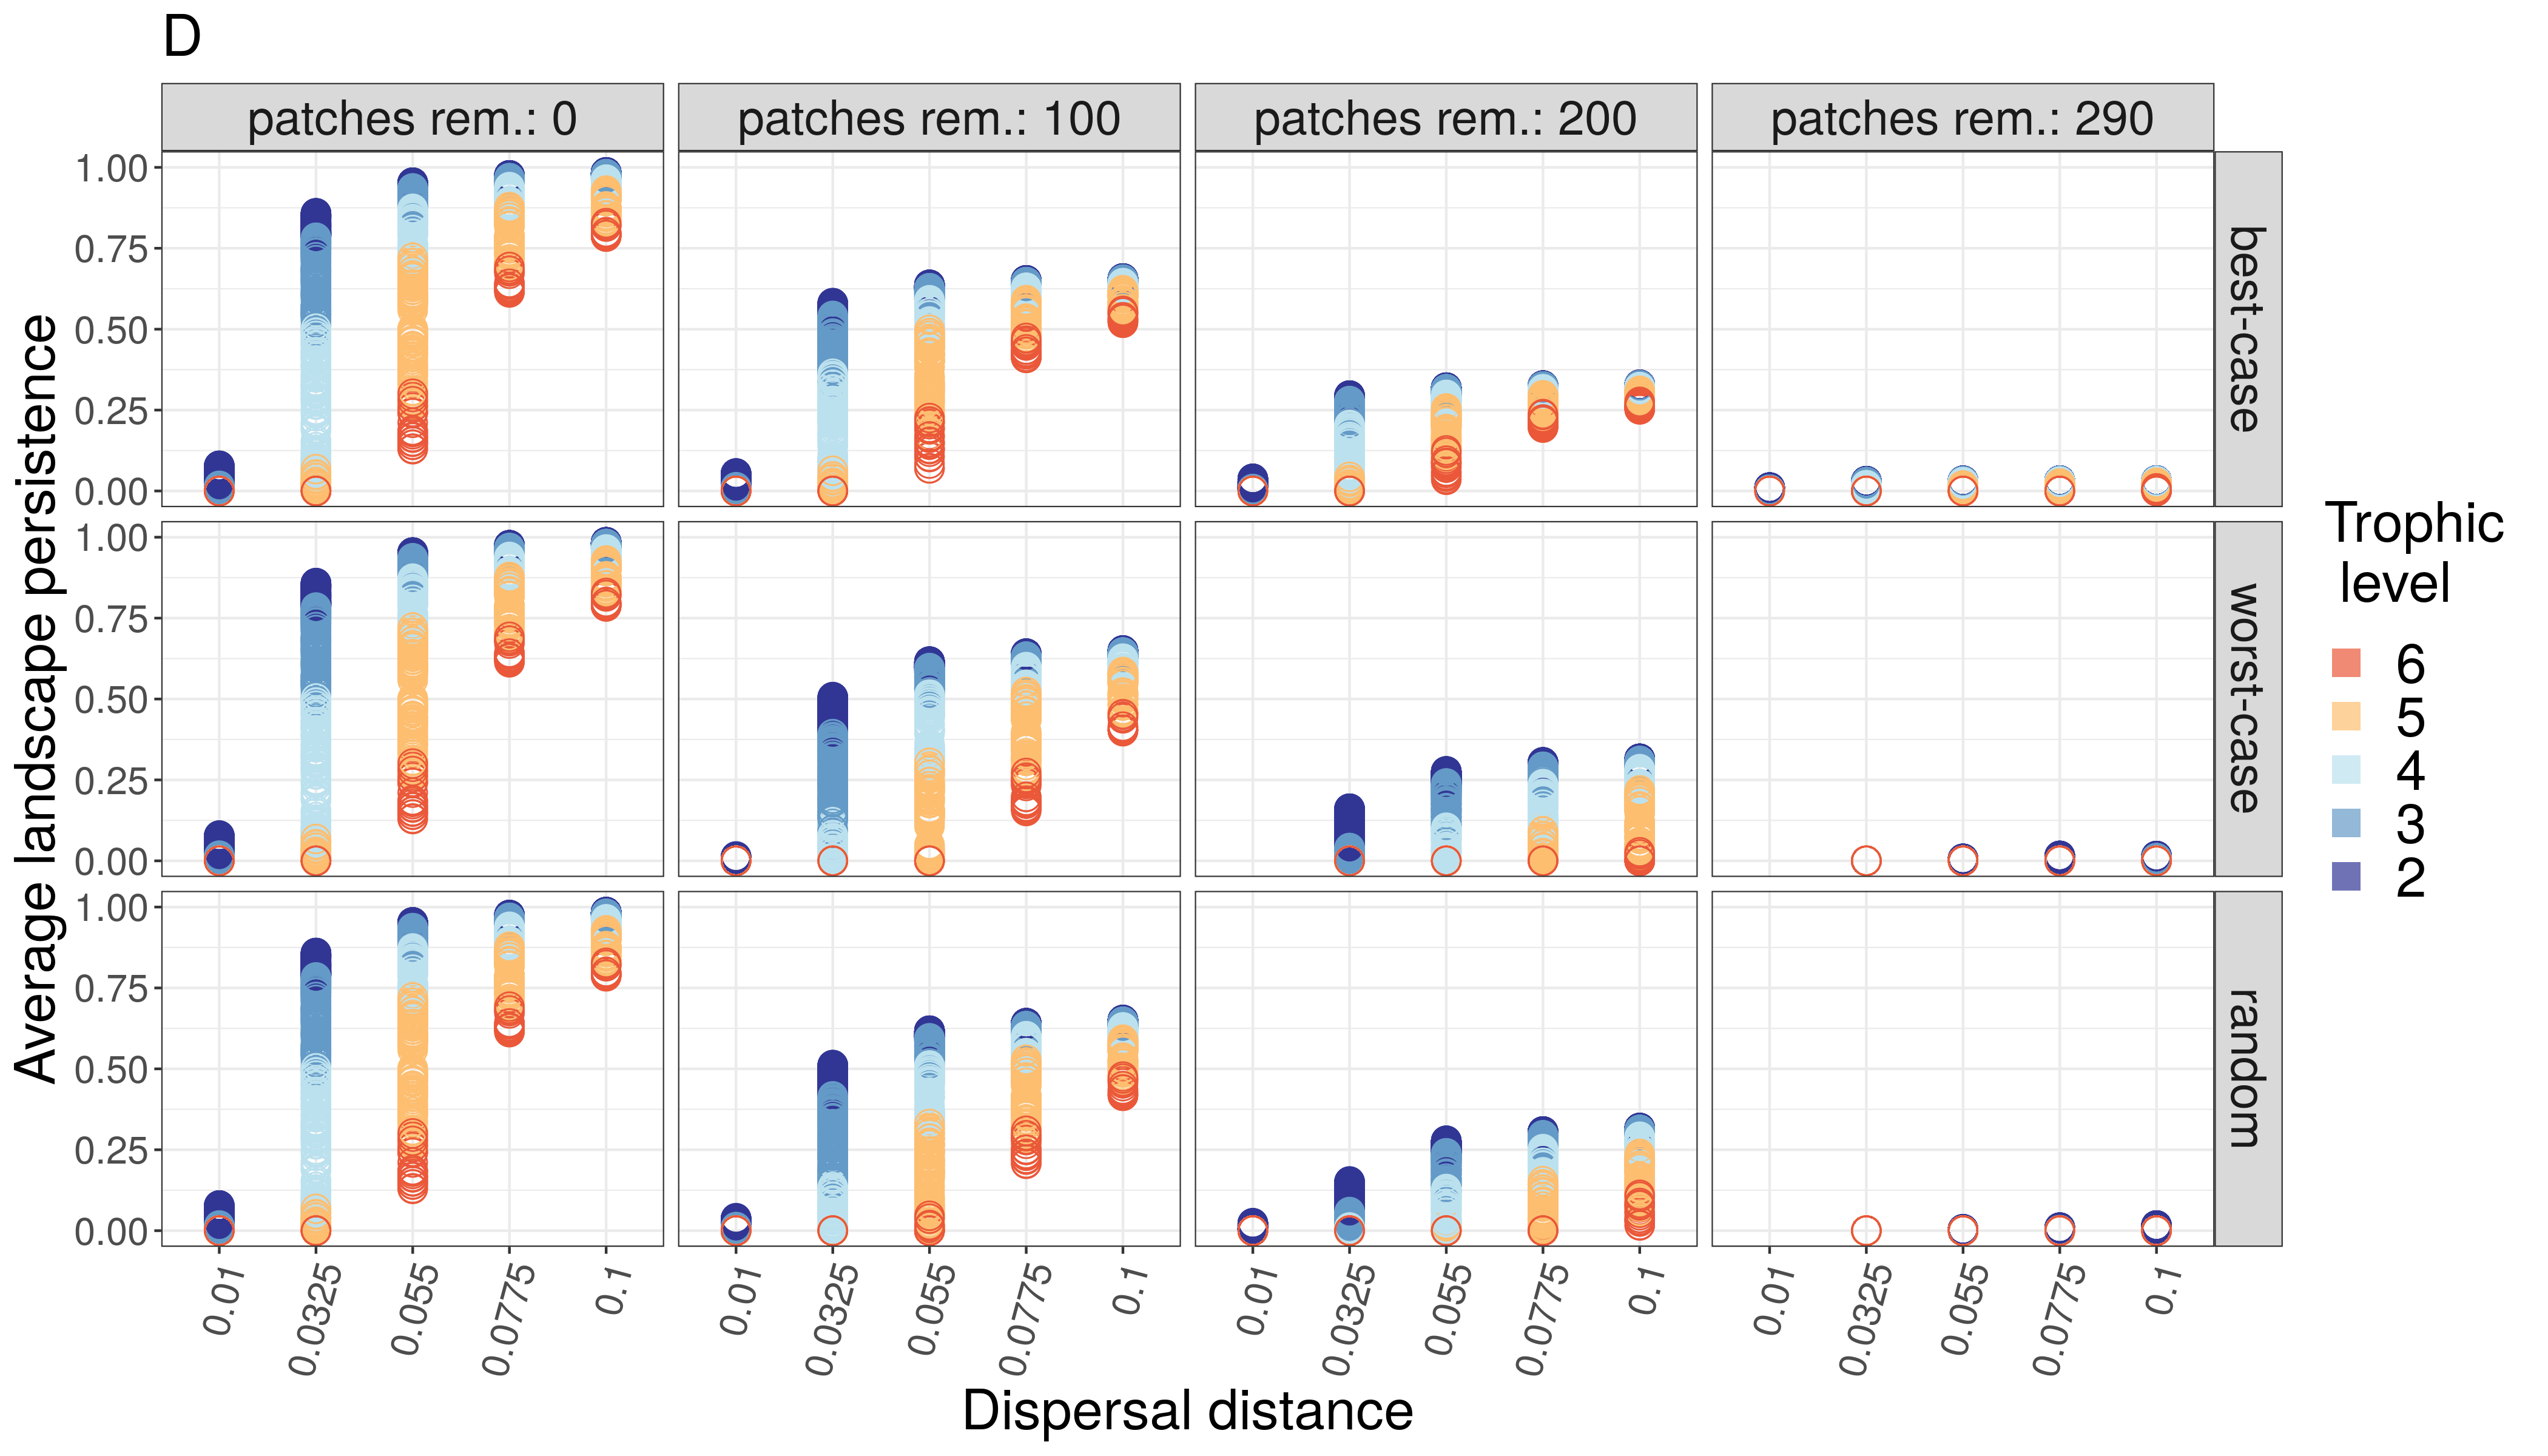
\includegraphics[width=0.8\textwidth,valign=t]{sump_Model_food_web_with_200_consumer_and_200_basal_species_basal_5_5.png}
  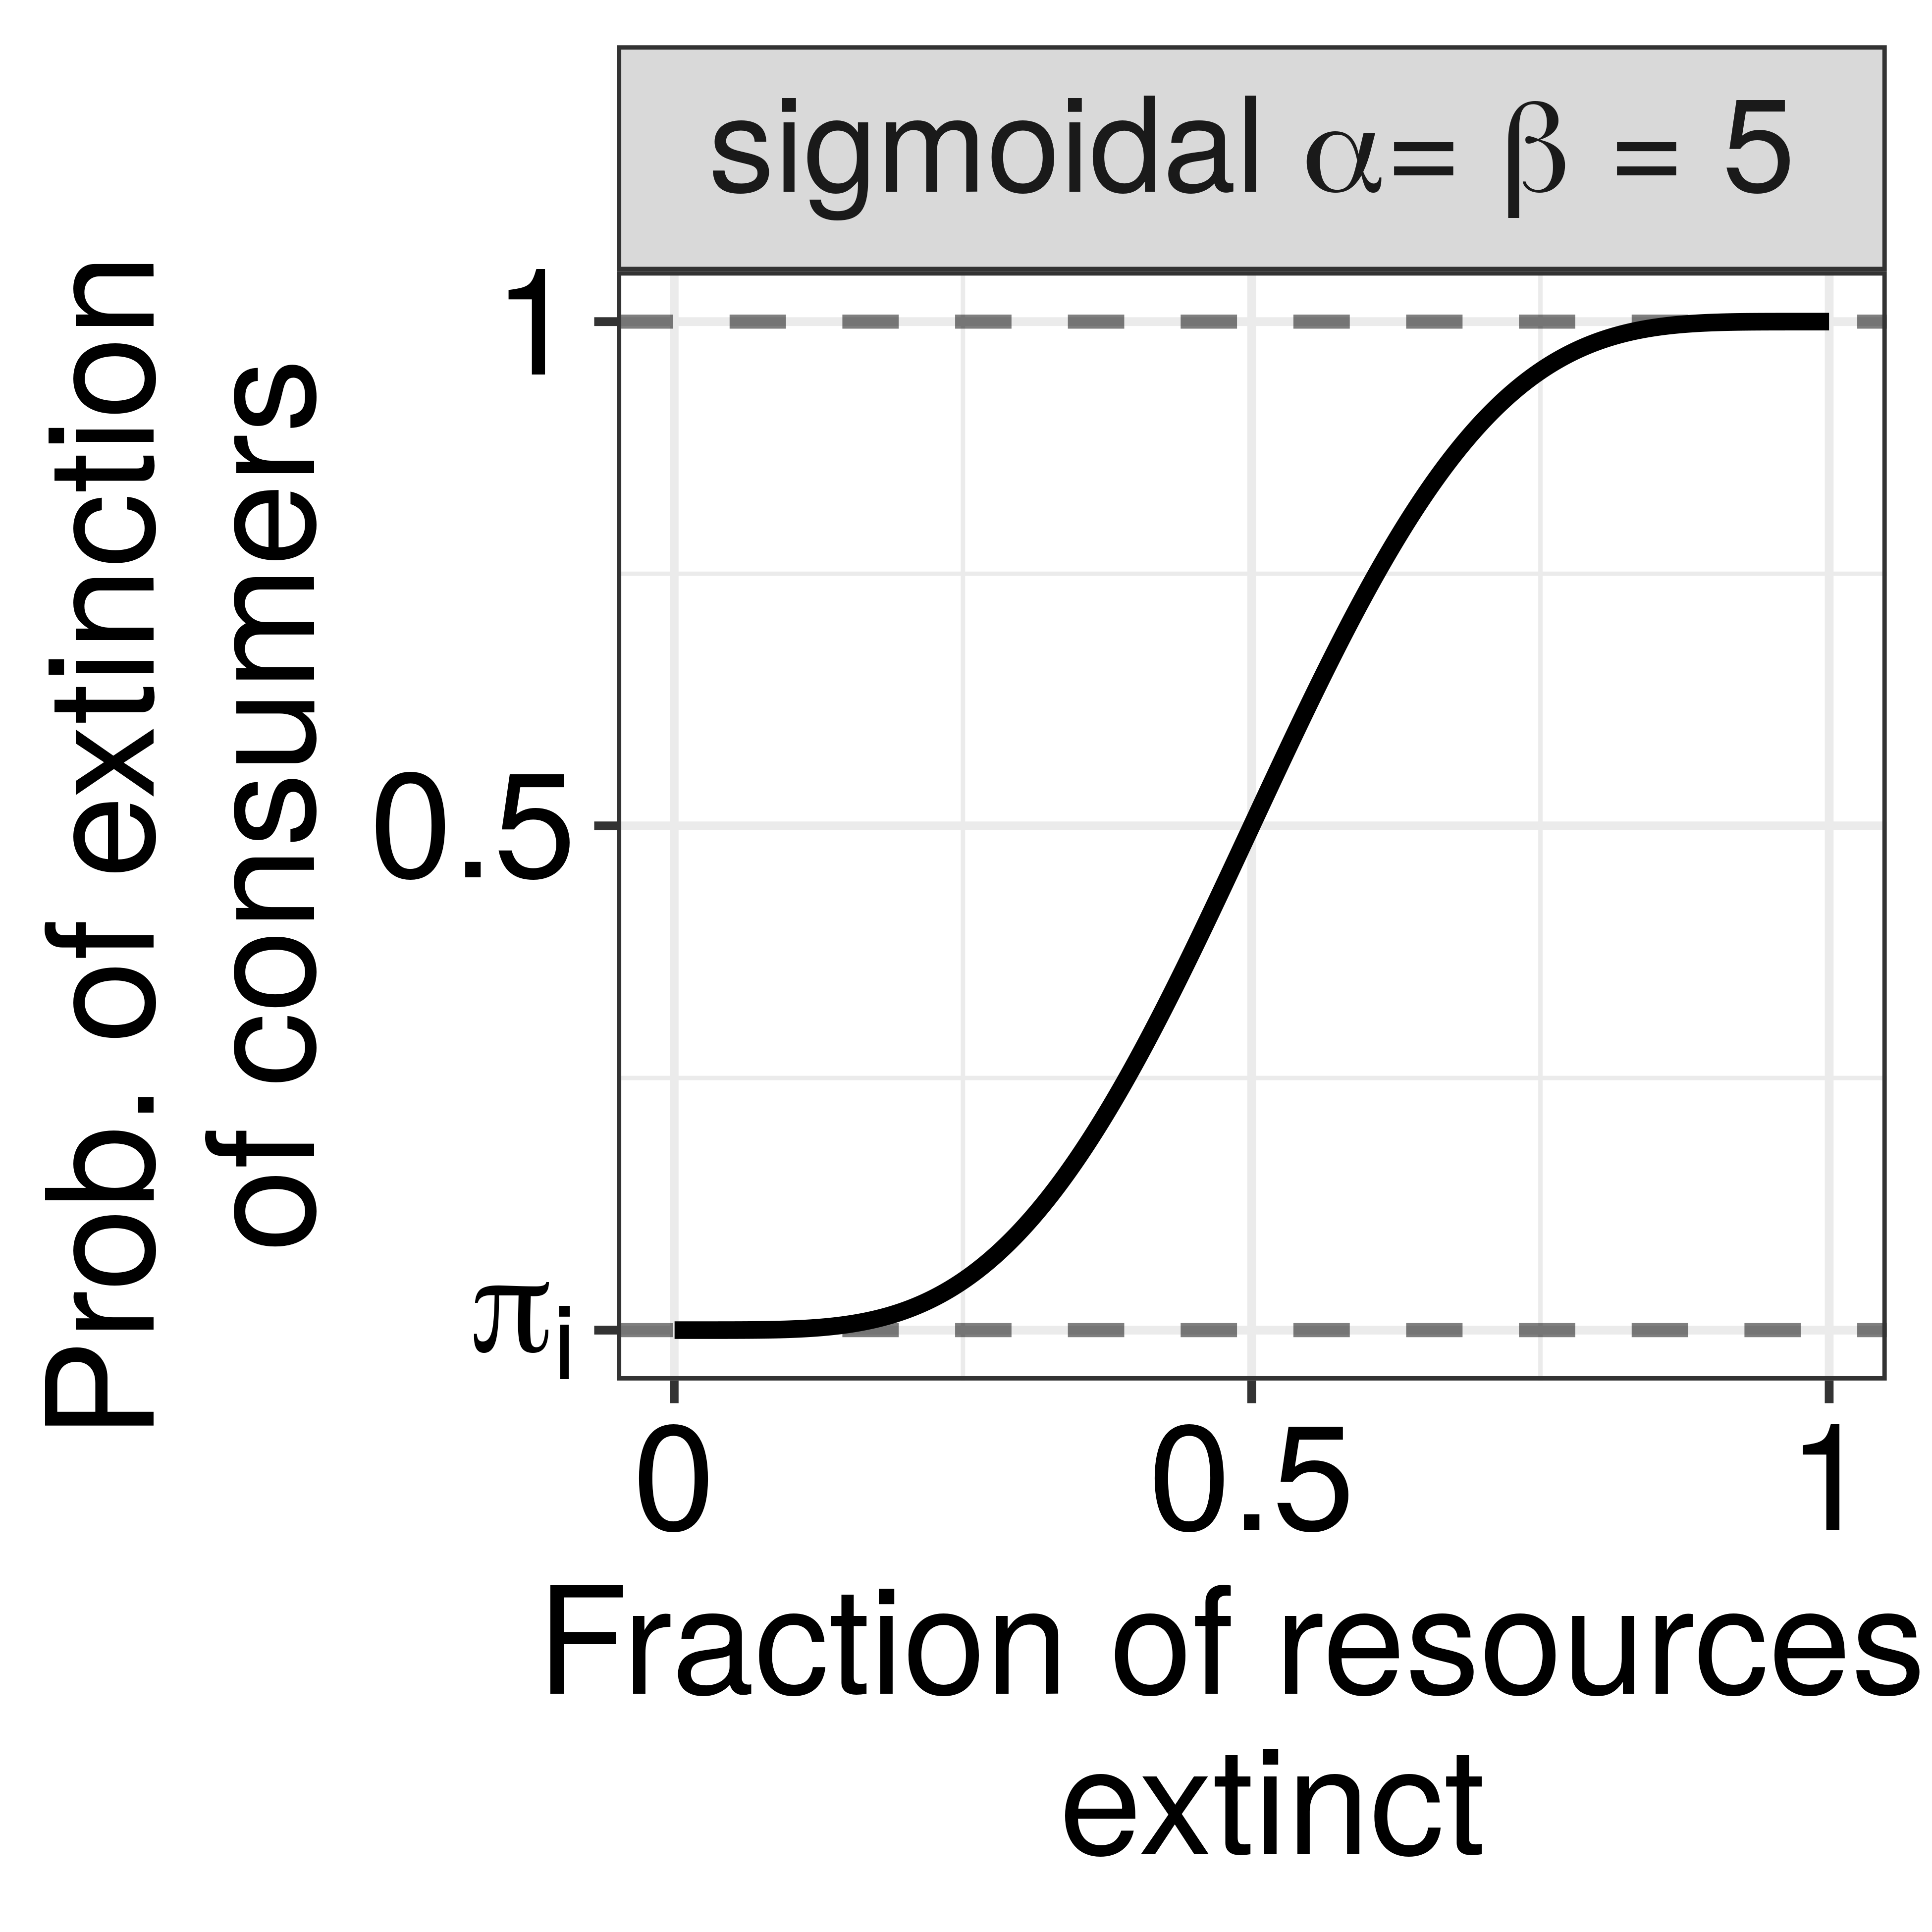
\includegraphics[width=0.19\textwidth,valign=t]{fform_5_5.png}
\caption{Figure continued.}   
\label{S_fig:patchloss_200_200_distance_2}
\end{figure}


\begin{figure}[!ht]
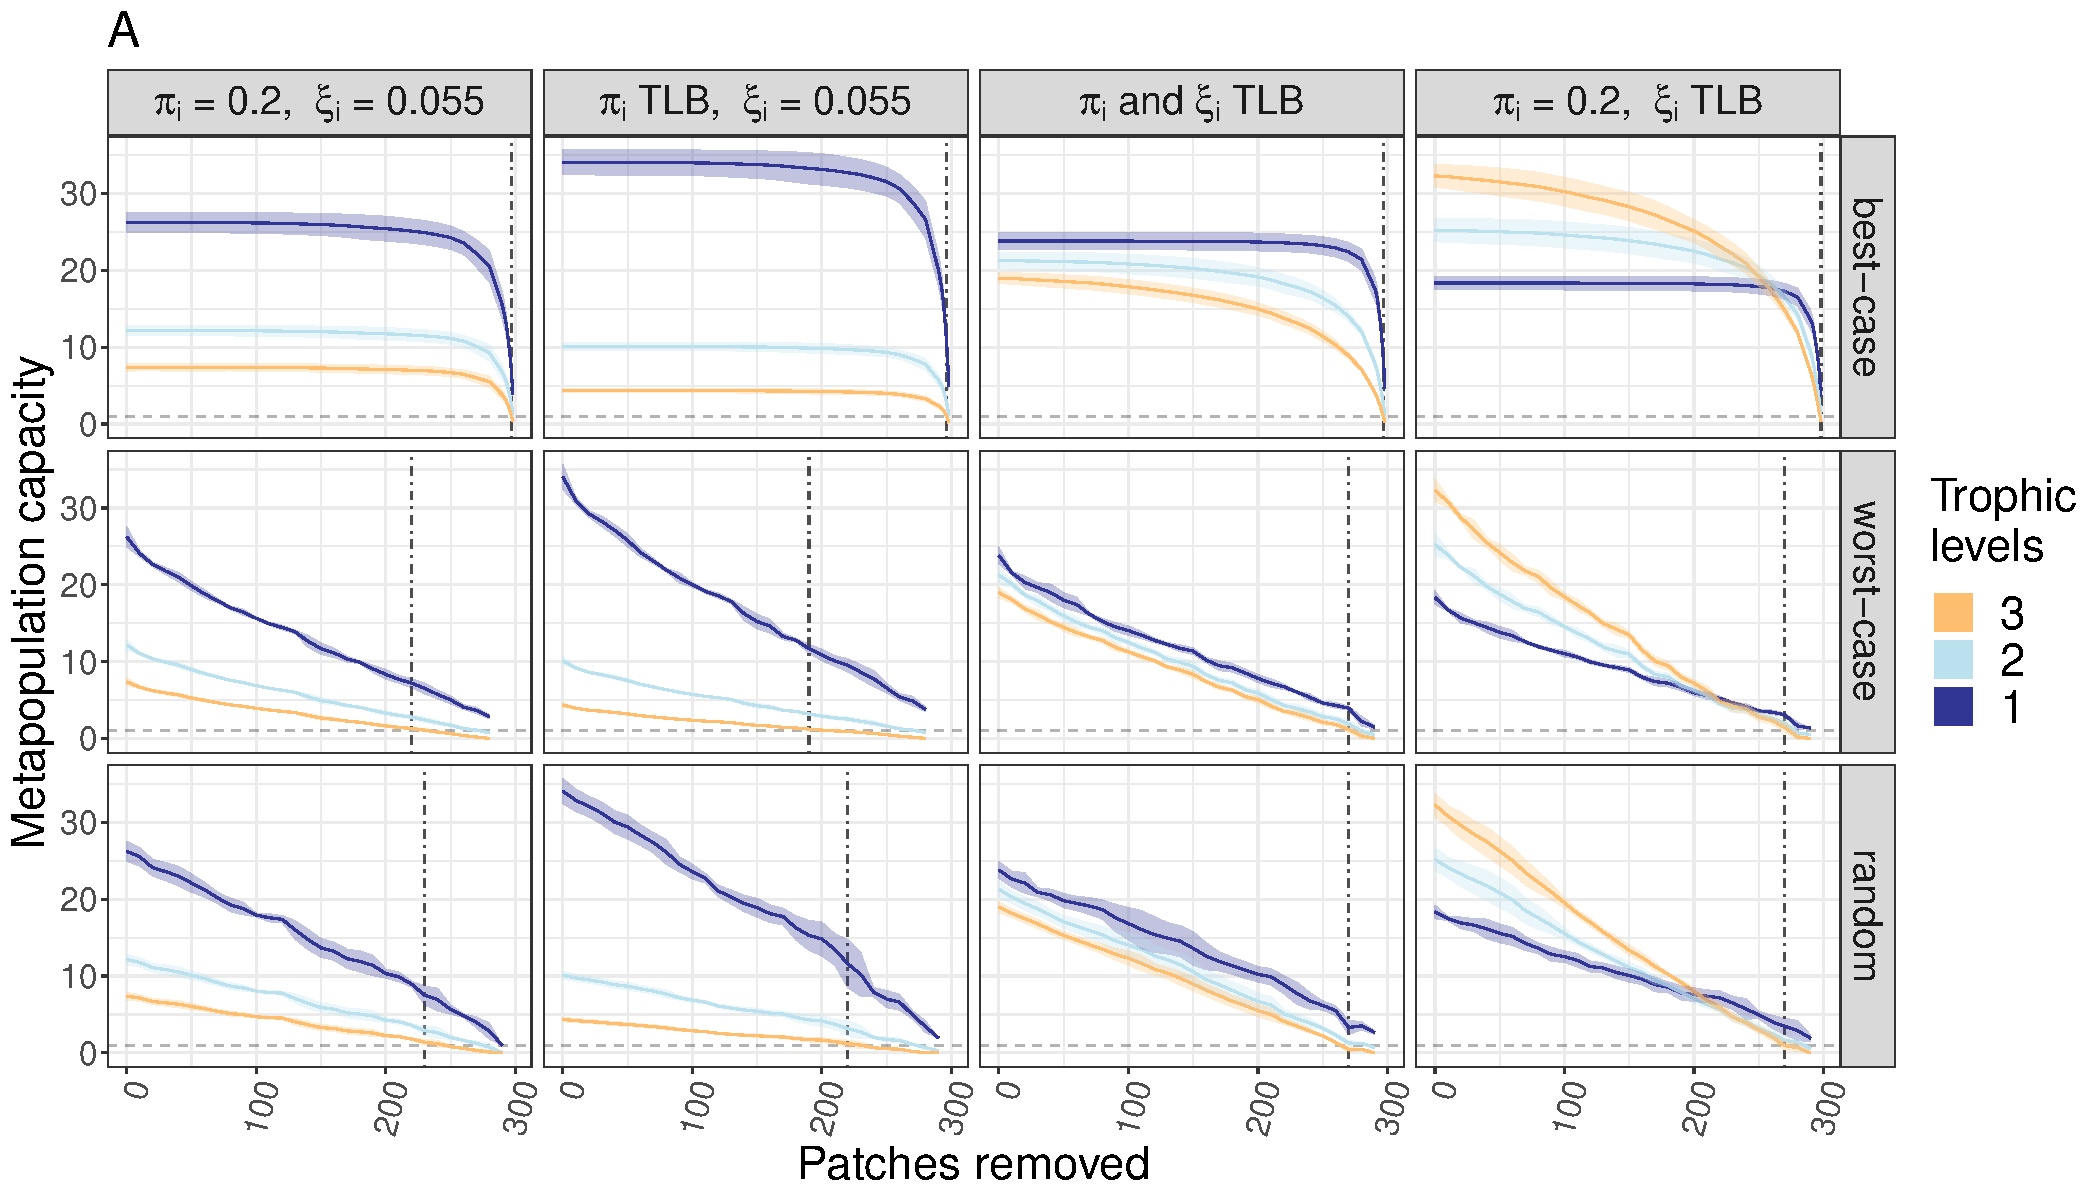
\includegraphics[width=0.8\textwidth,valign=t]{lambda_Serengeti_food_web_with_32_consumer_and_129_basal_species_basal_1_1.pdf}
  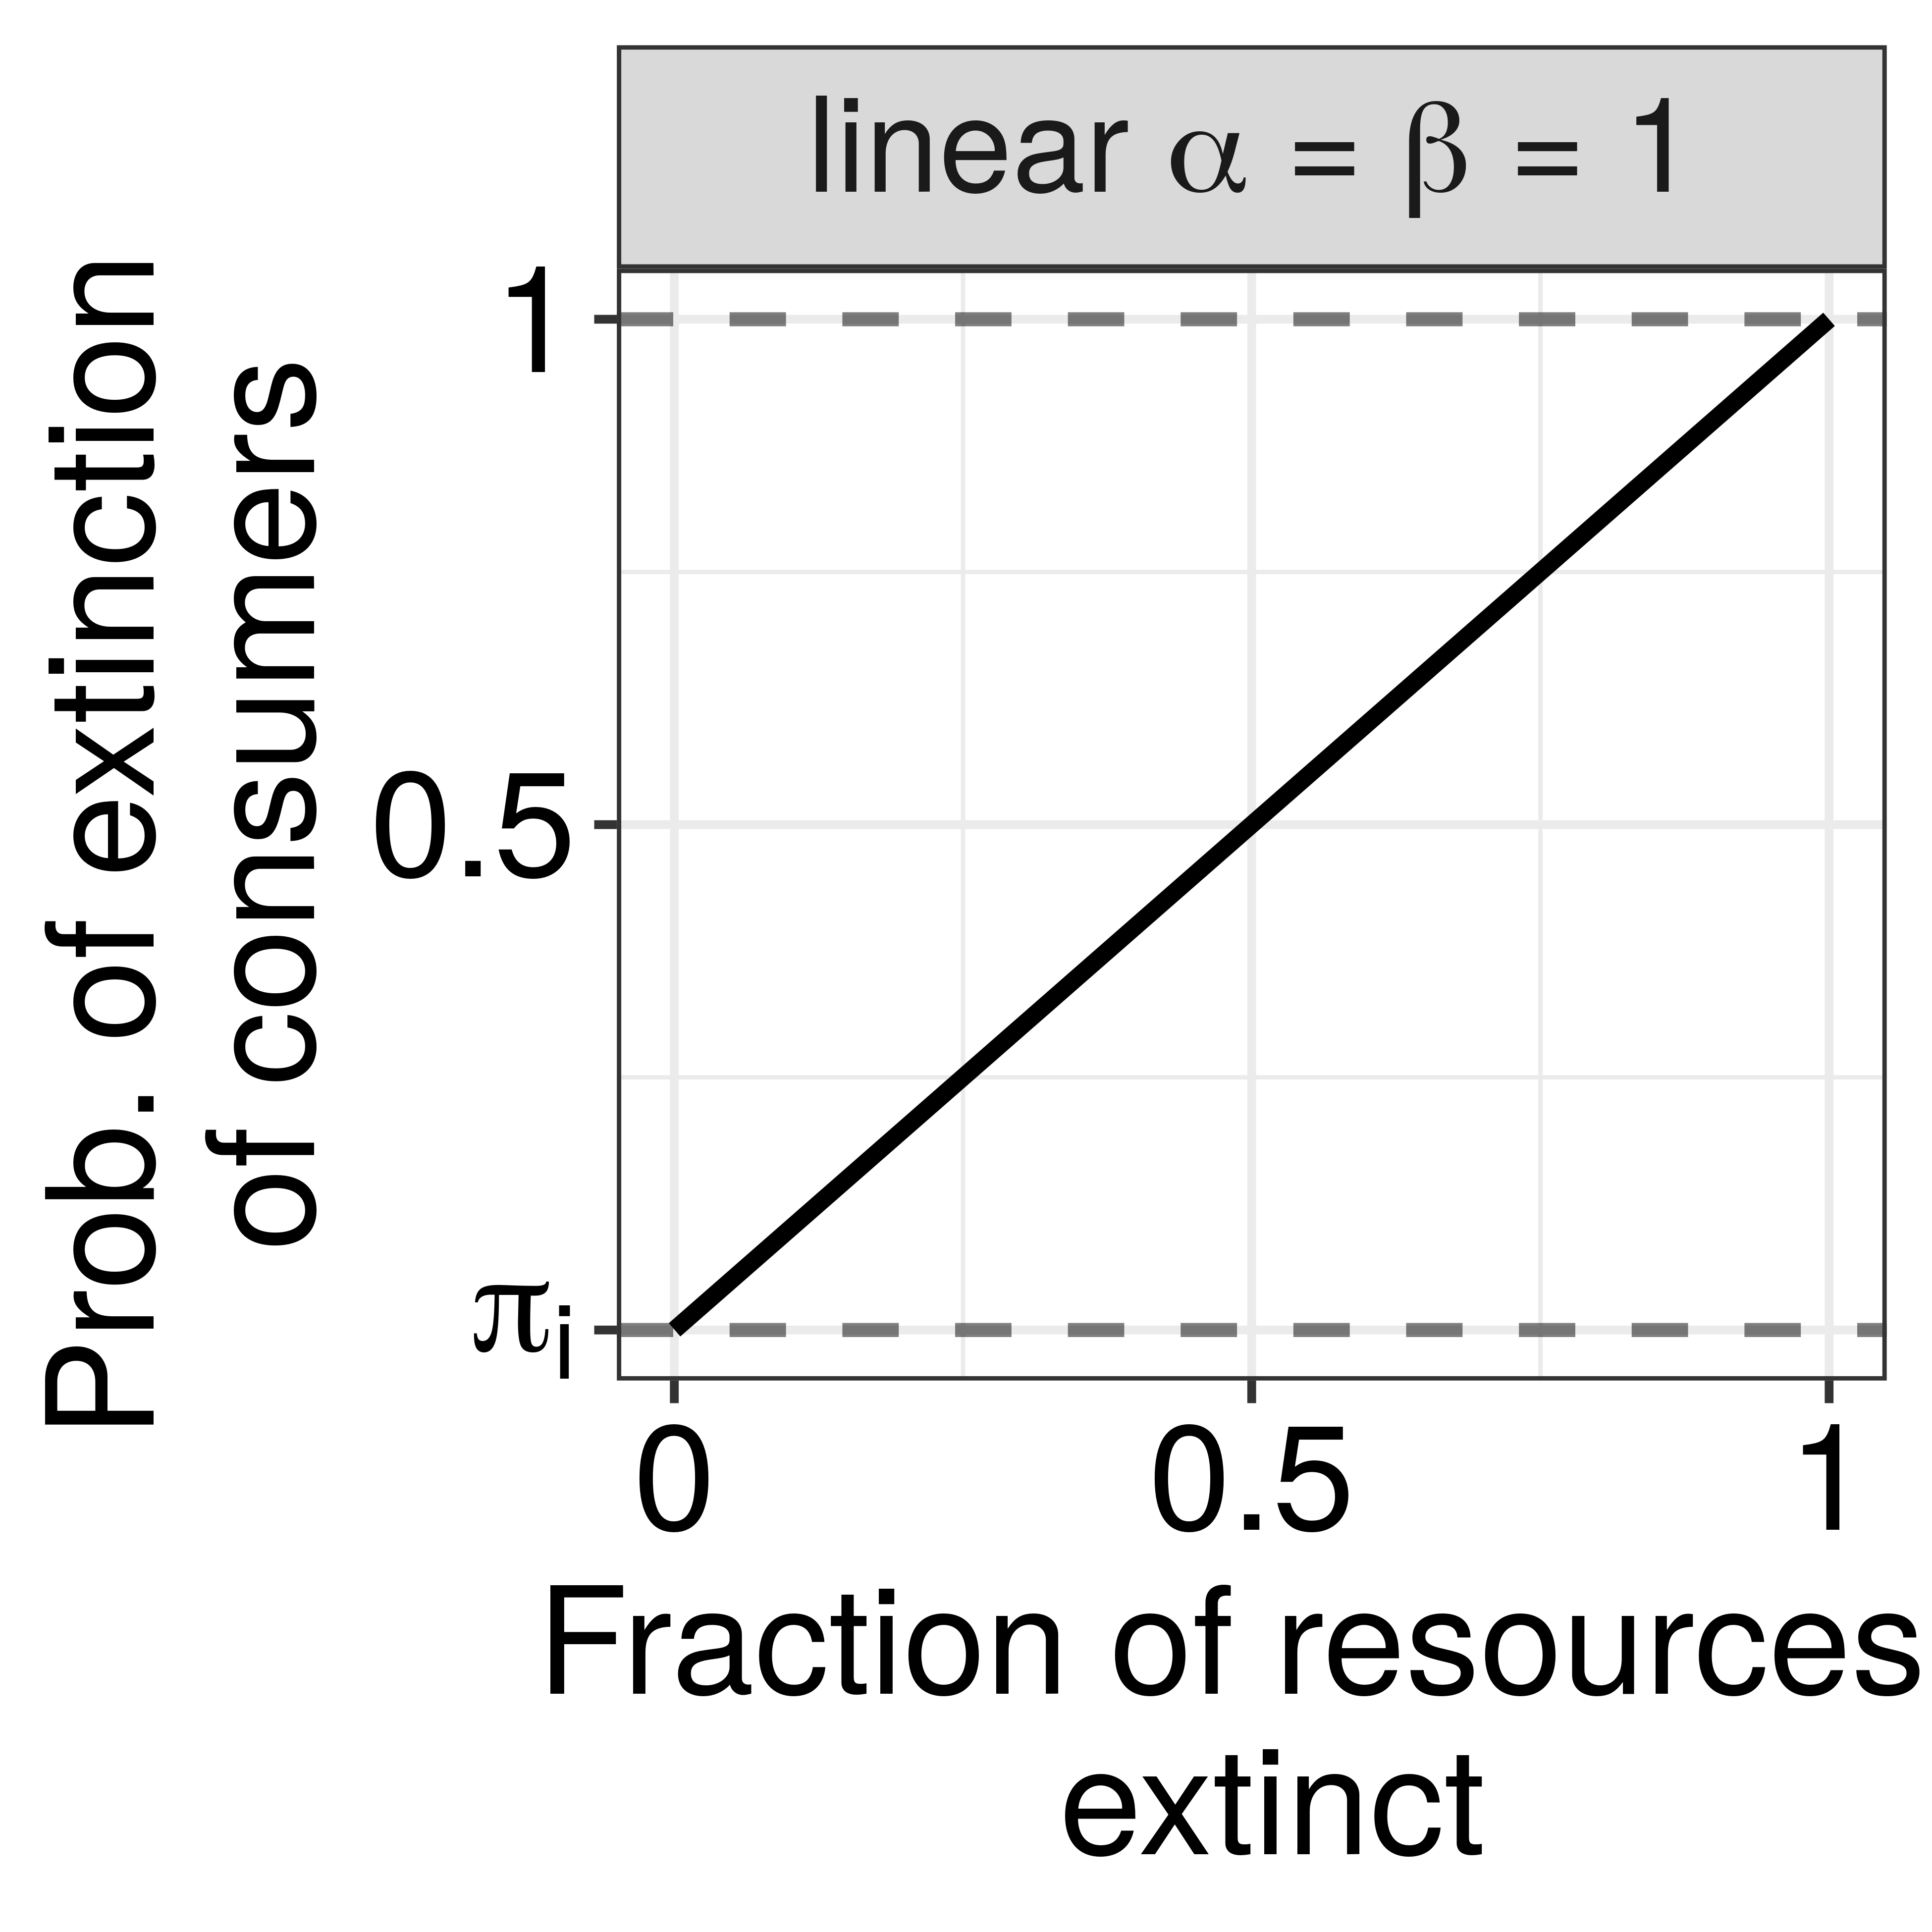
\includegraphics[width=0.19\textwidth,valign=t]{fform_1_1.png}
  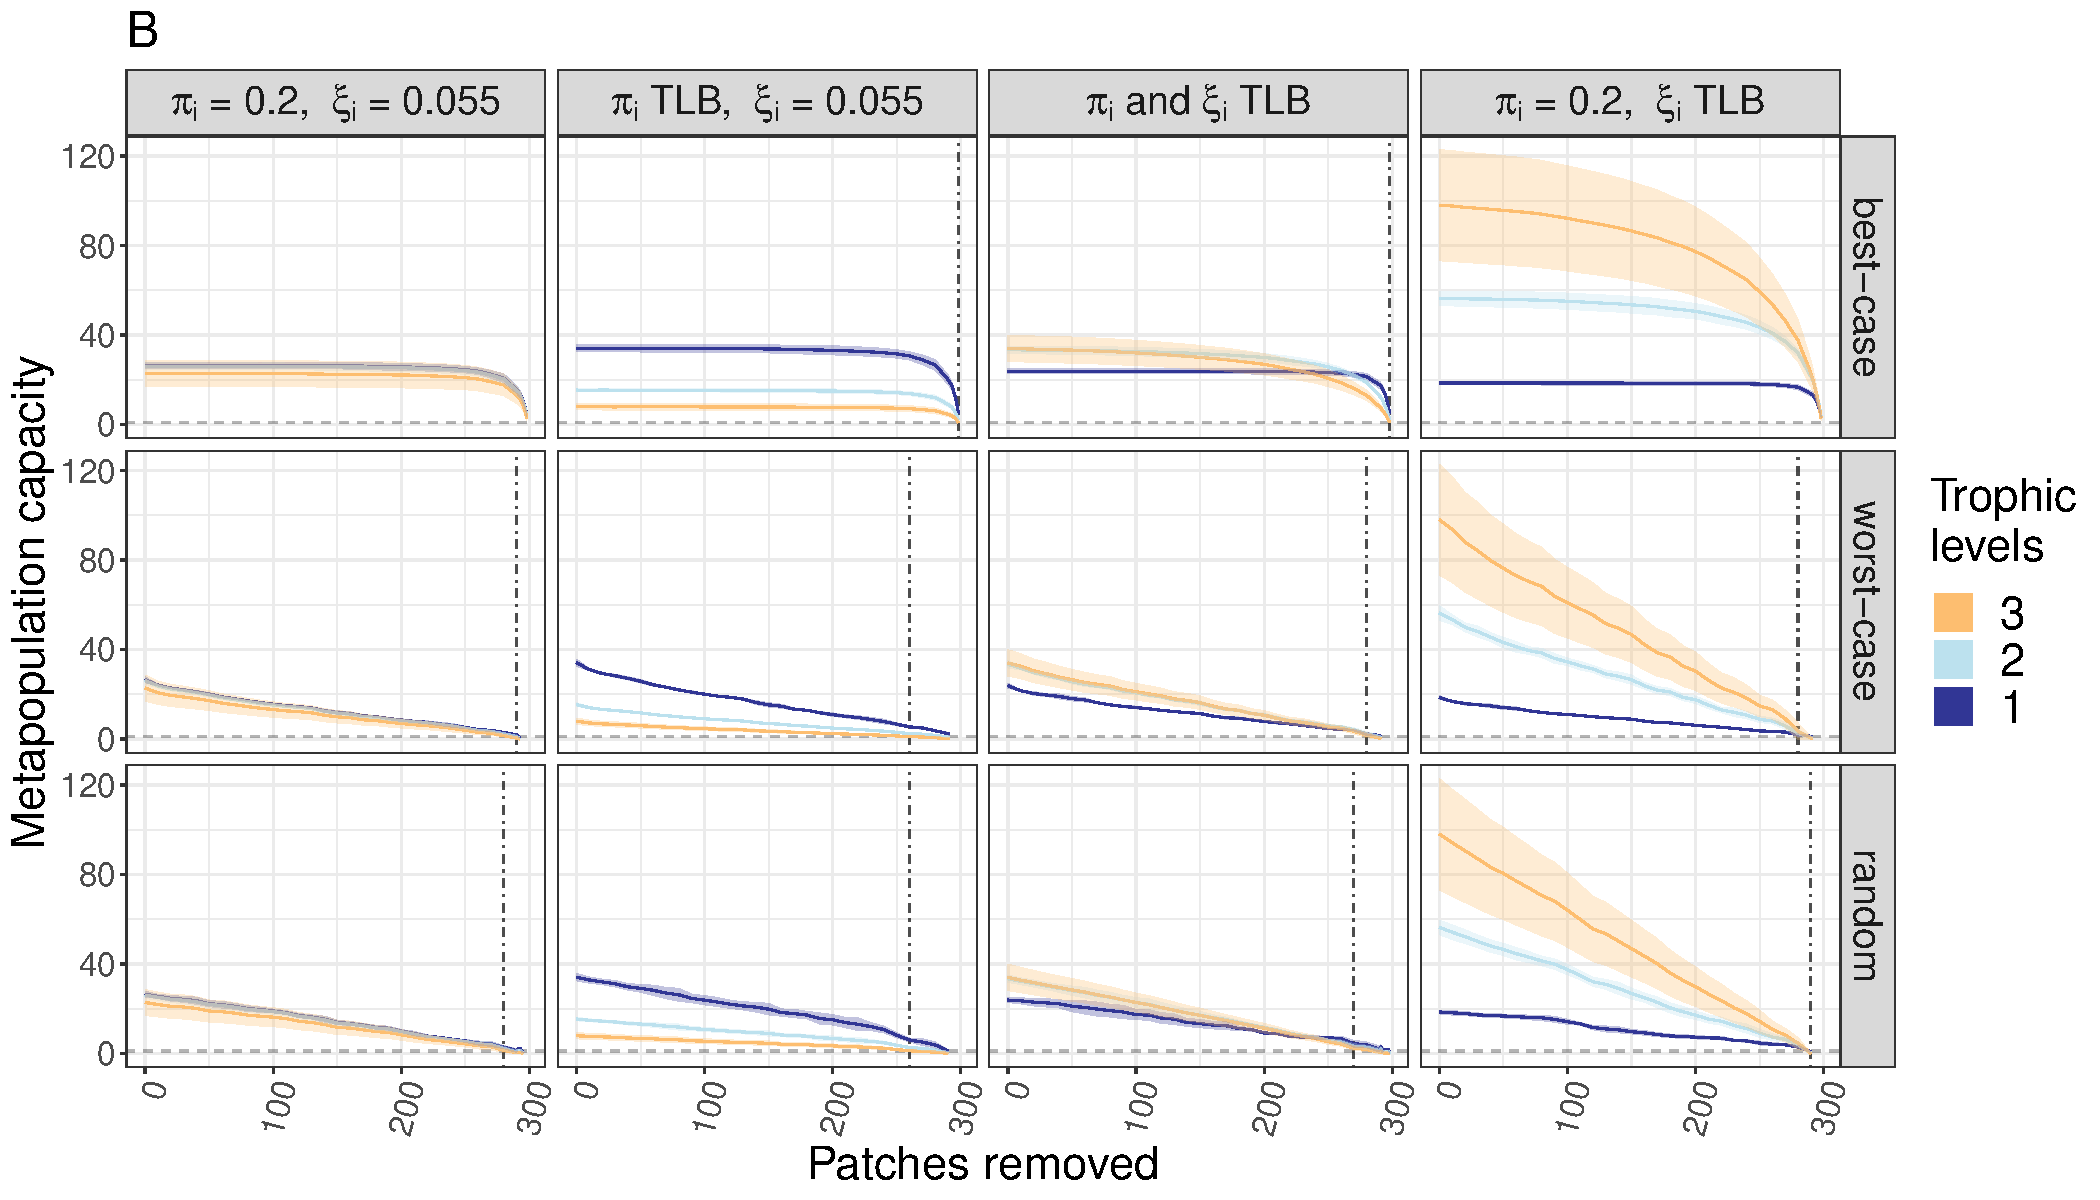
\includegraphics[width=0.8\textwidth,valign=t]{lambda_Serengeti_food_web_with_32_consumer_and_129_basal_species_basal_5_1.pdf}
    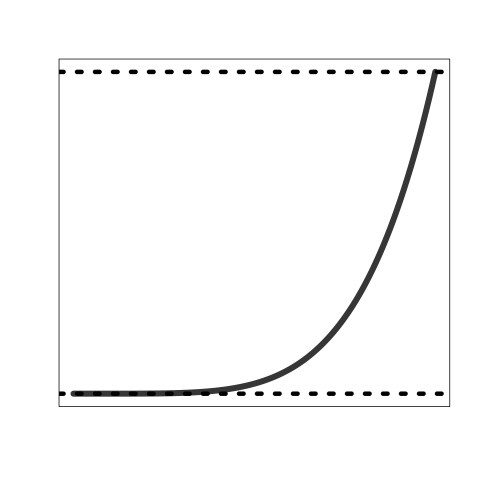
\includegraphics[width=0.19\textwidth,valign=t]{fform_5_1.png}
\caption{As Figure \ref{S_fig:patchloss_350_50_1}, but for the Serengeti food web.} 
\label{S_fig:patchloss_Serengeti_TLB_1}
\end{figure}

\begin{figure}\ContinuedFloat
 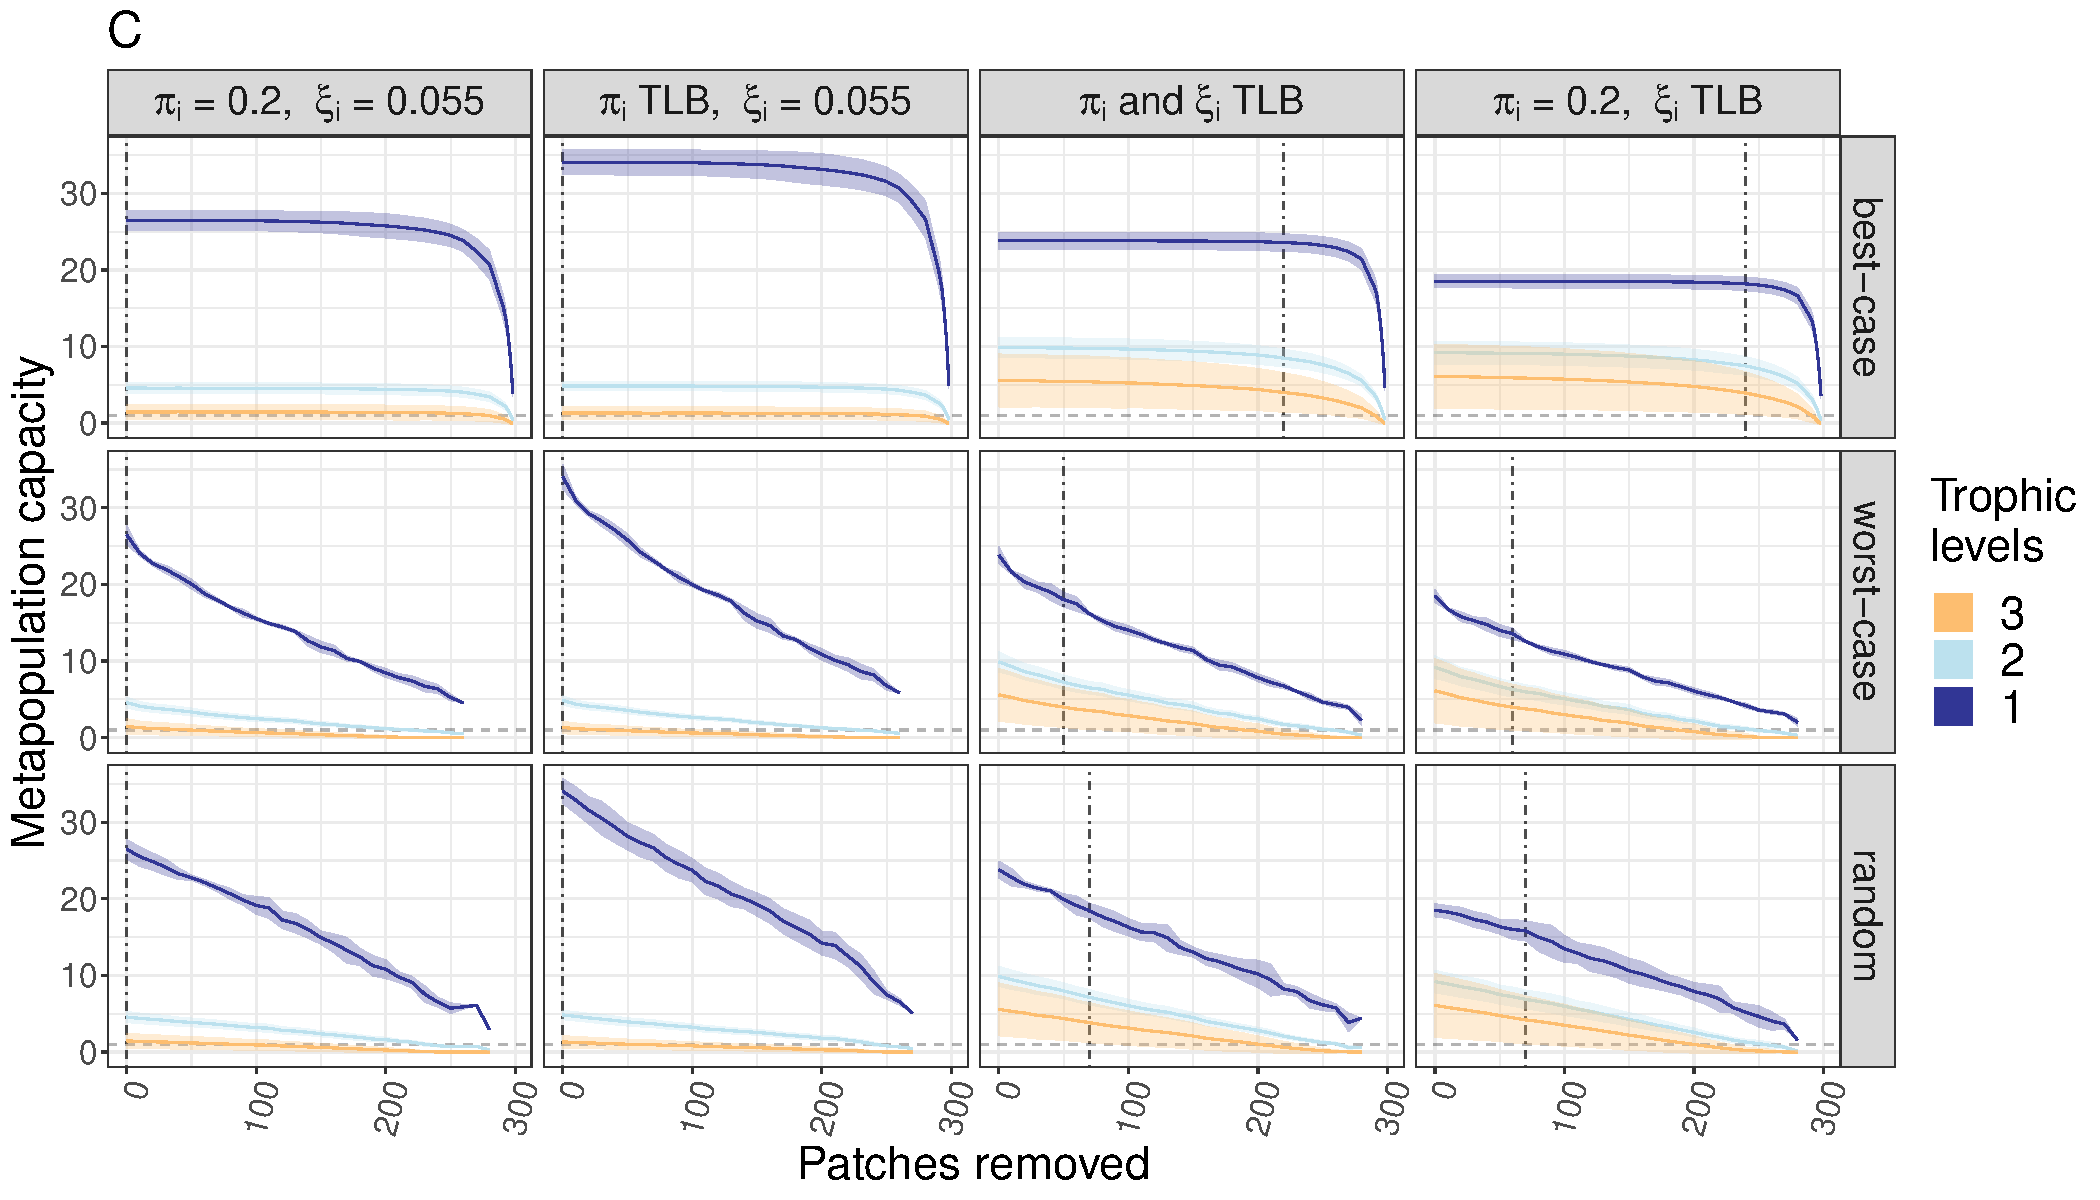
\includegraphics[width=0.8\textwidth,valign=t]{lambda_Serengeti_food_web_with_32_consumer_and_129_basal_species_basal_1_5.pdf}
  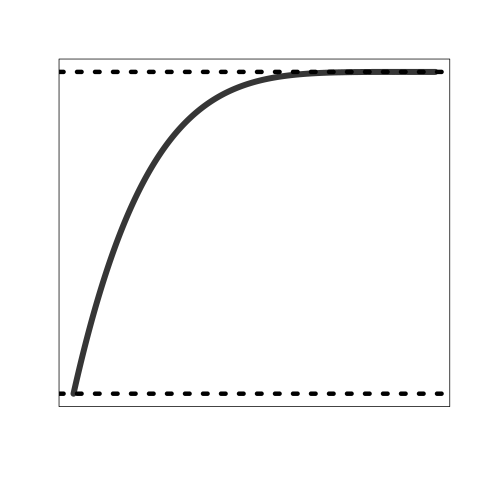
\includegraphics[width=0.19\textwidth,valign=t]{fform_1_5.png}
  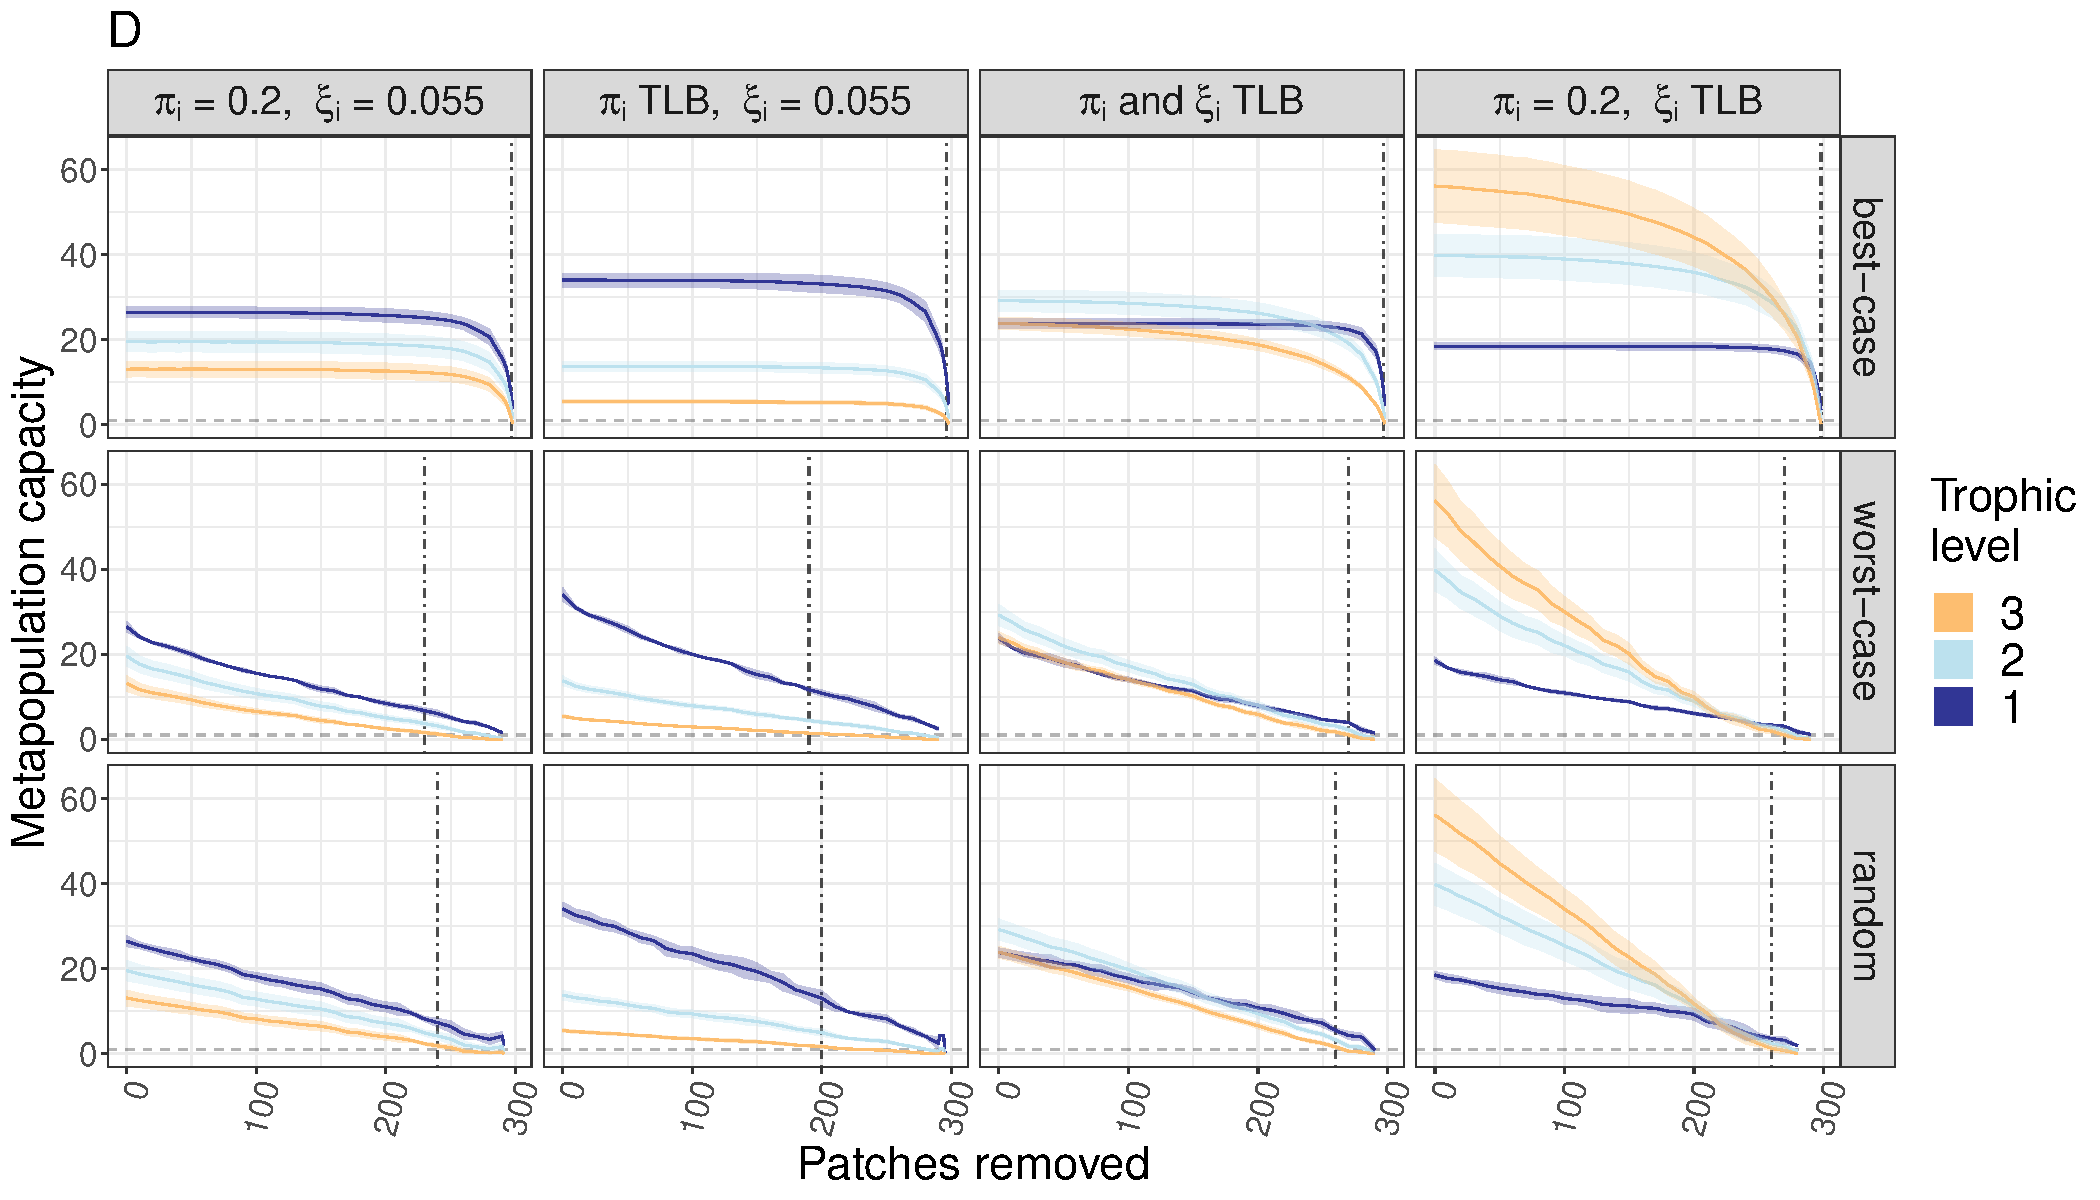
\includegraphics[width=0.8\textwidth,valign=t]{lambda_Serengeti_food_web_with_32_consumer_and_129_basal_species_basal_5_5.pdf}
  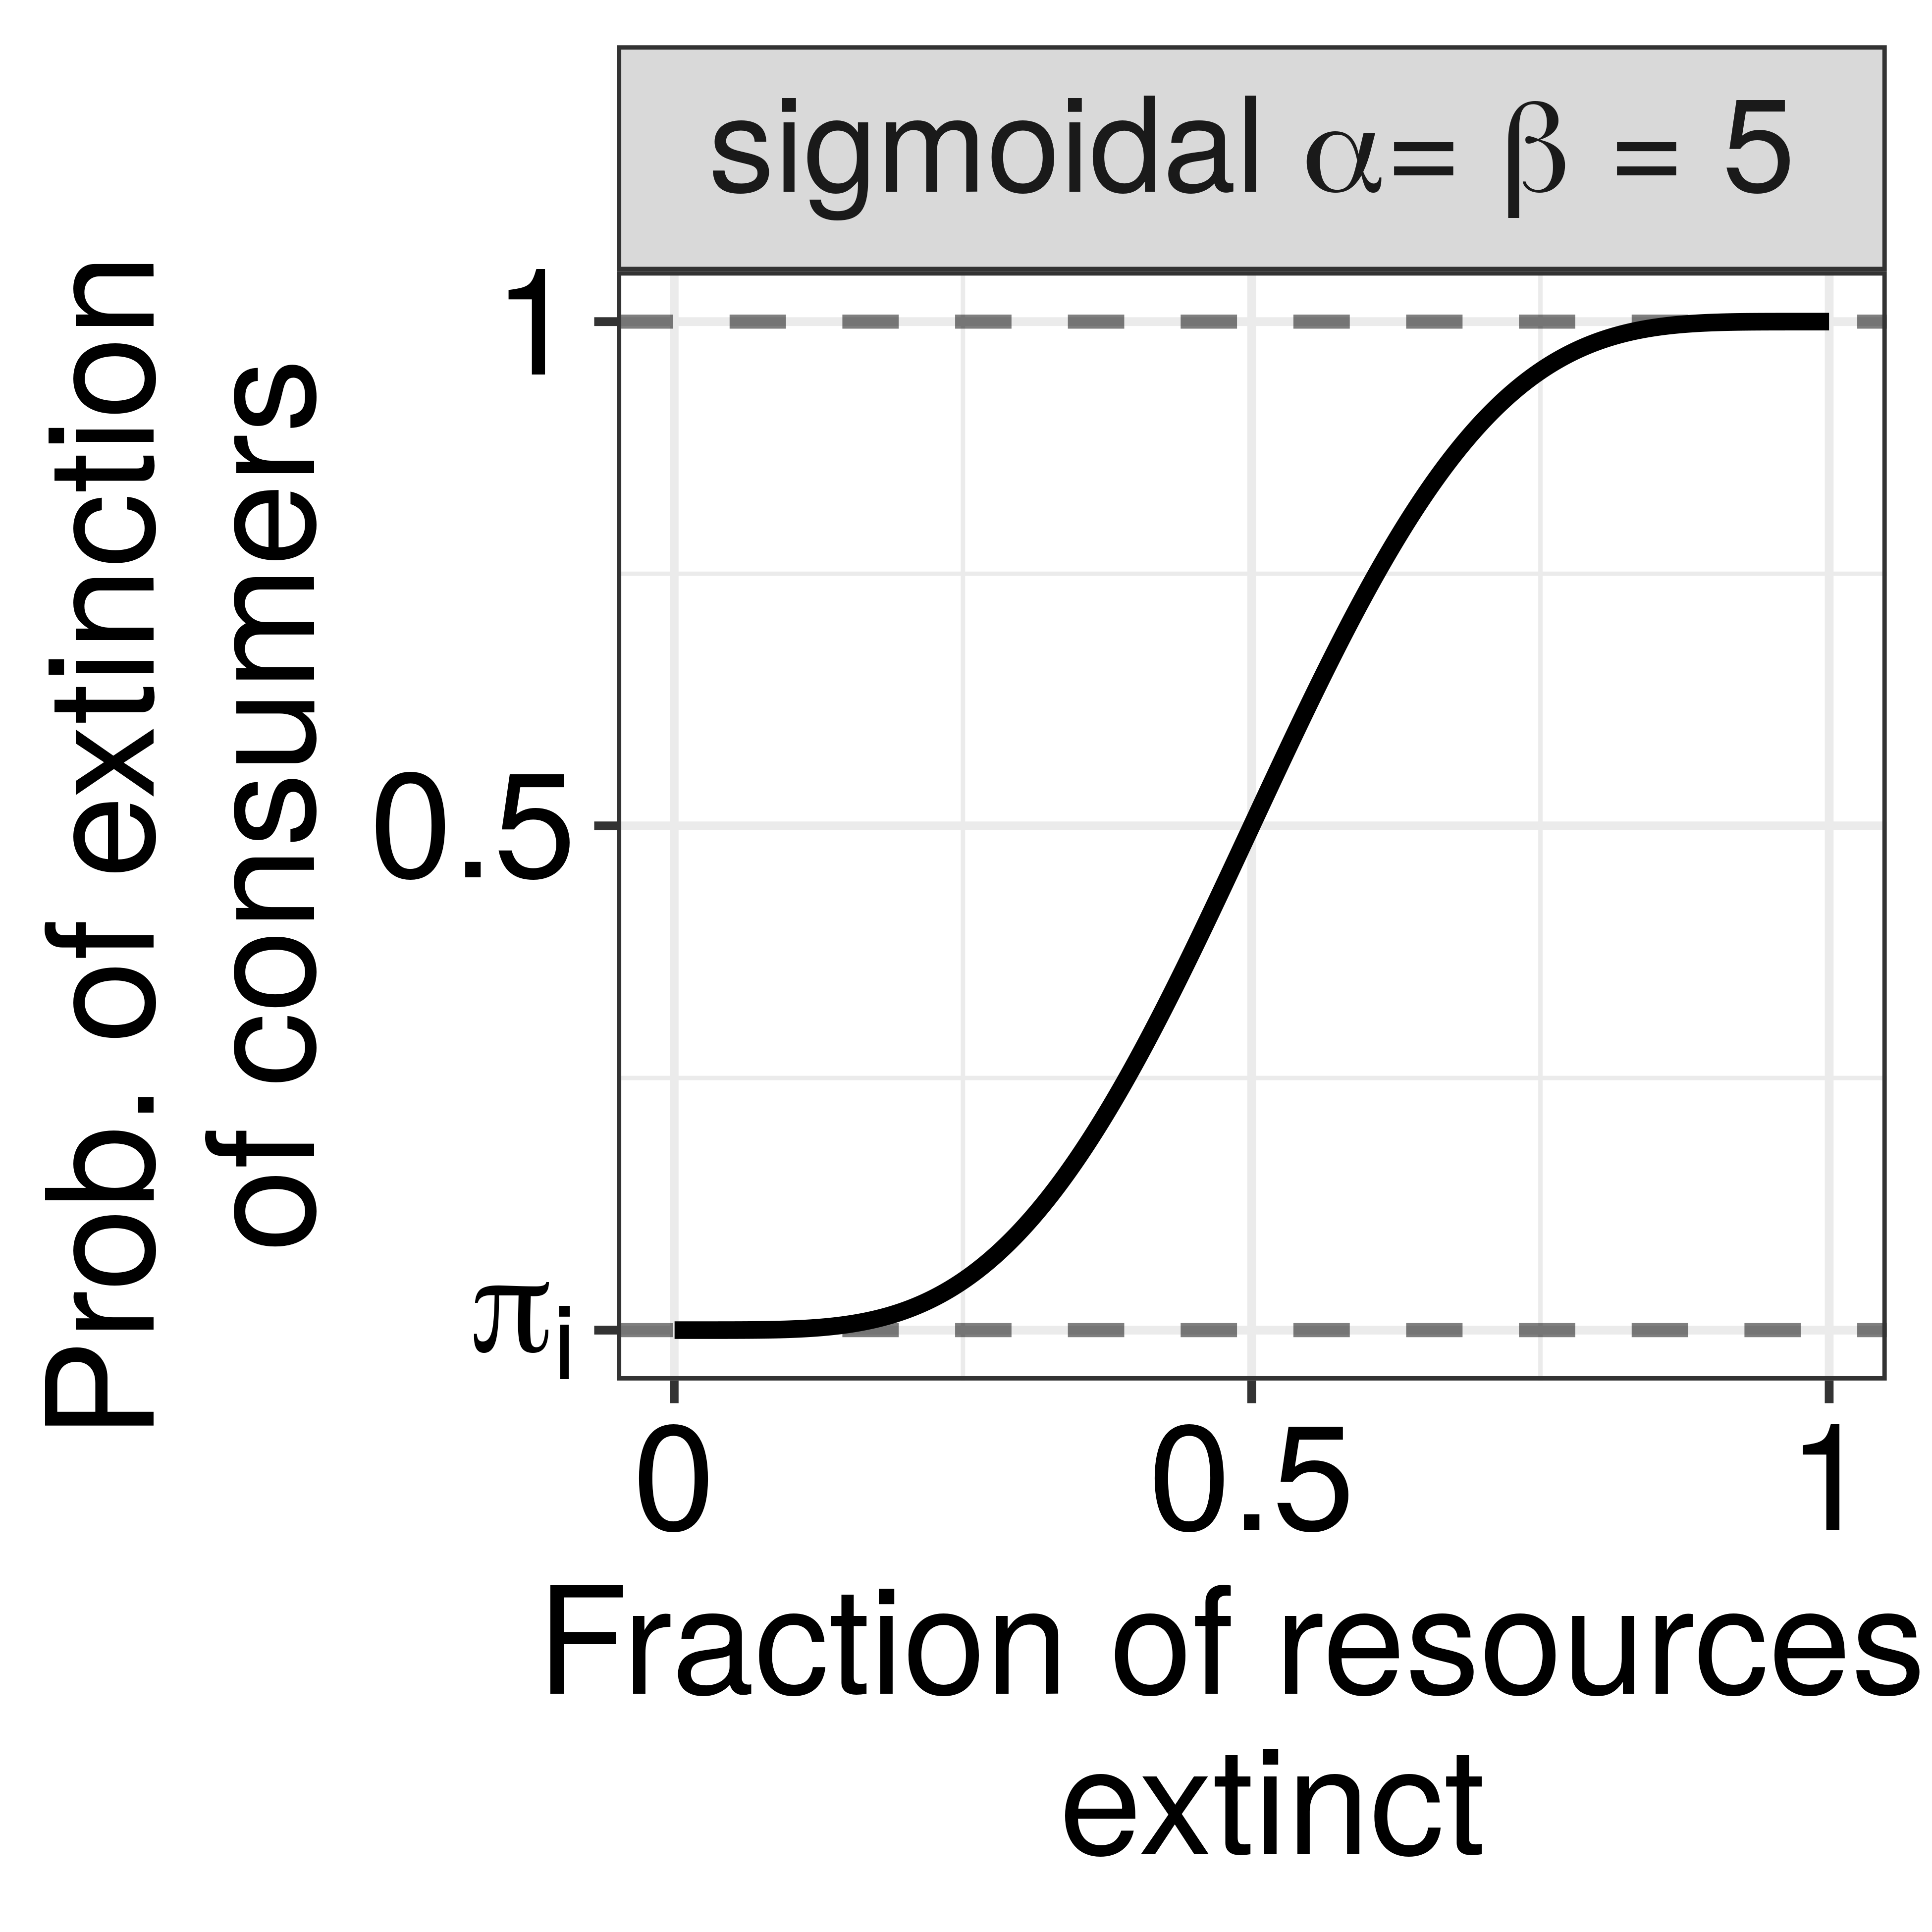
\includegraphics[width=0.19\textwidth,valign=t]{fform_5_5.png}
  \caption{Figure continued.}
\label{S_fig:patchloss_Serengeti_TLB_2}
\end{figure}

\begin{figure}
  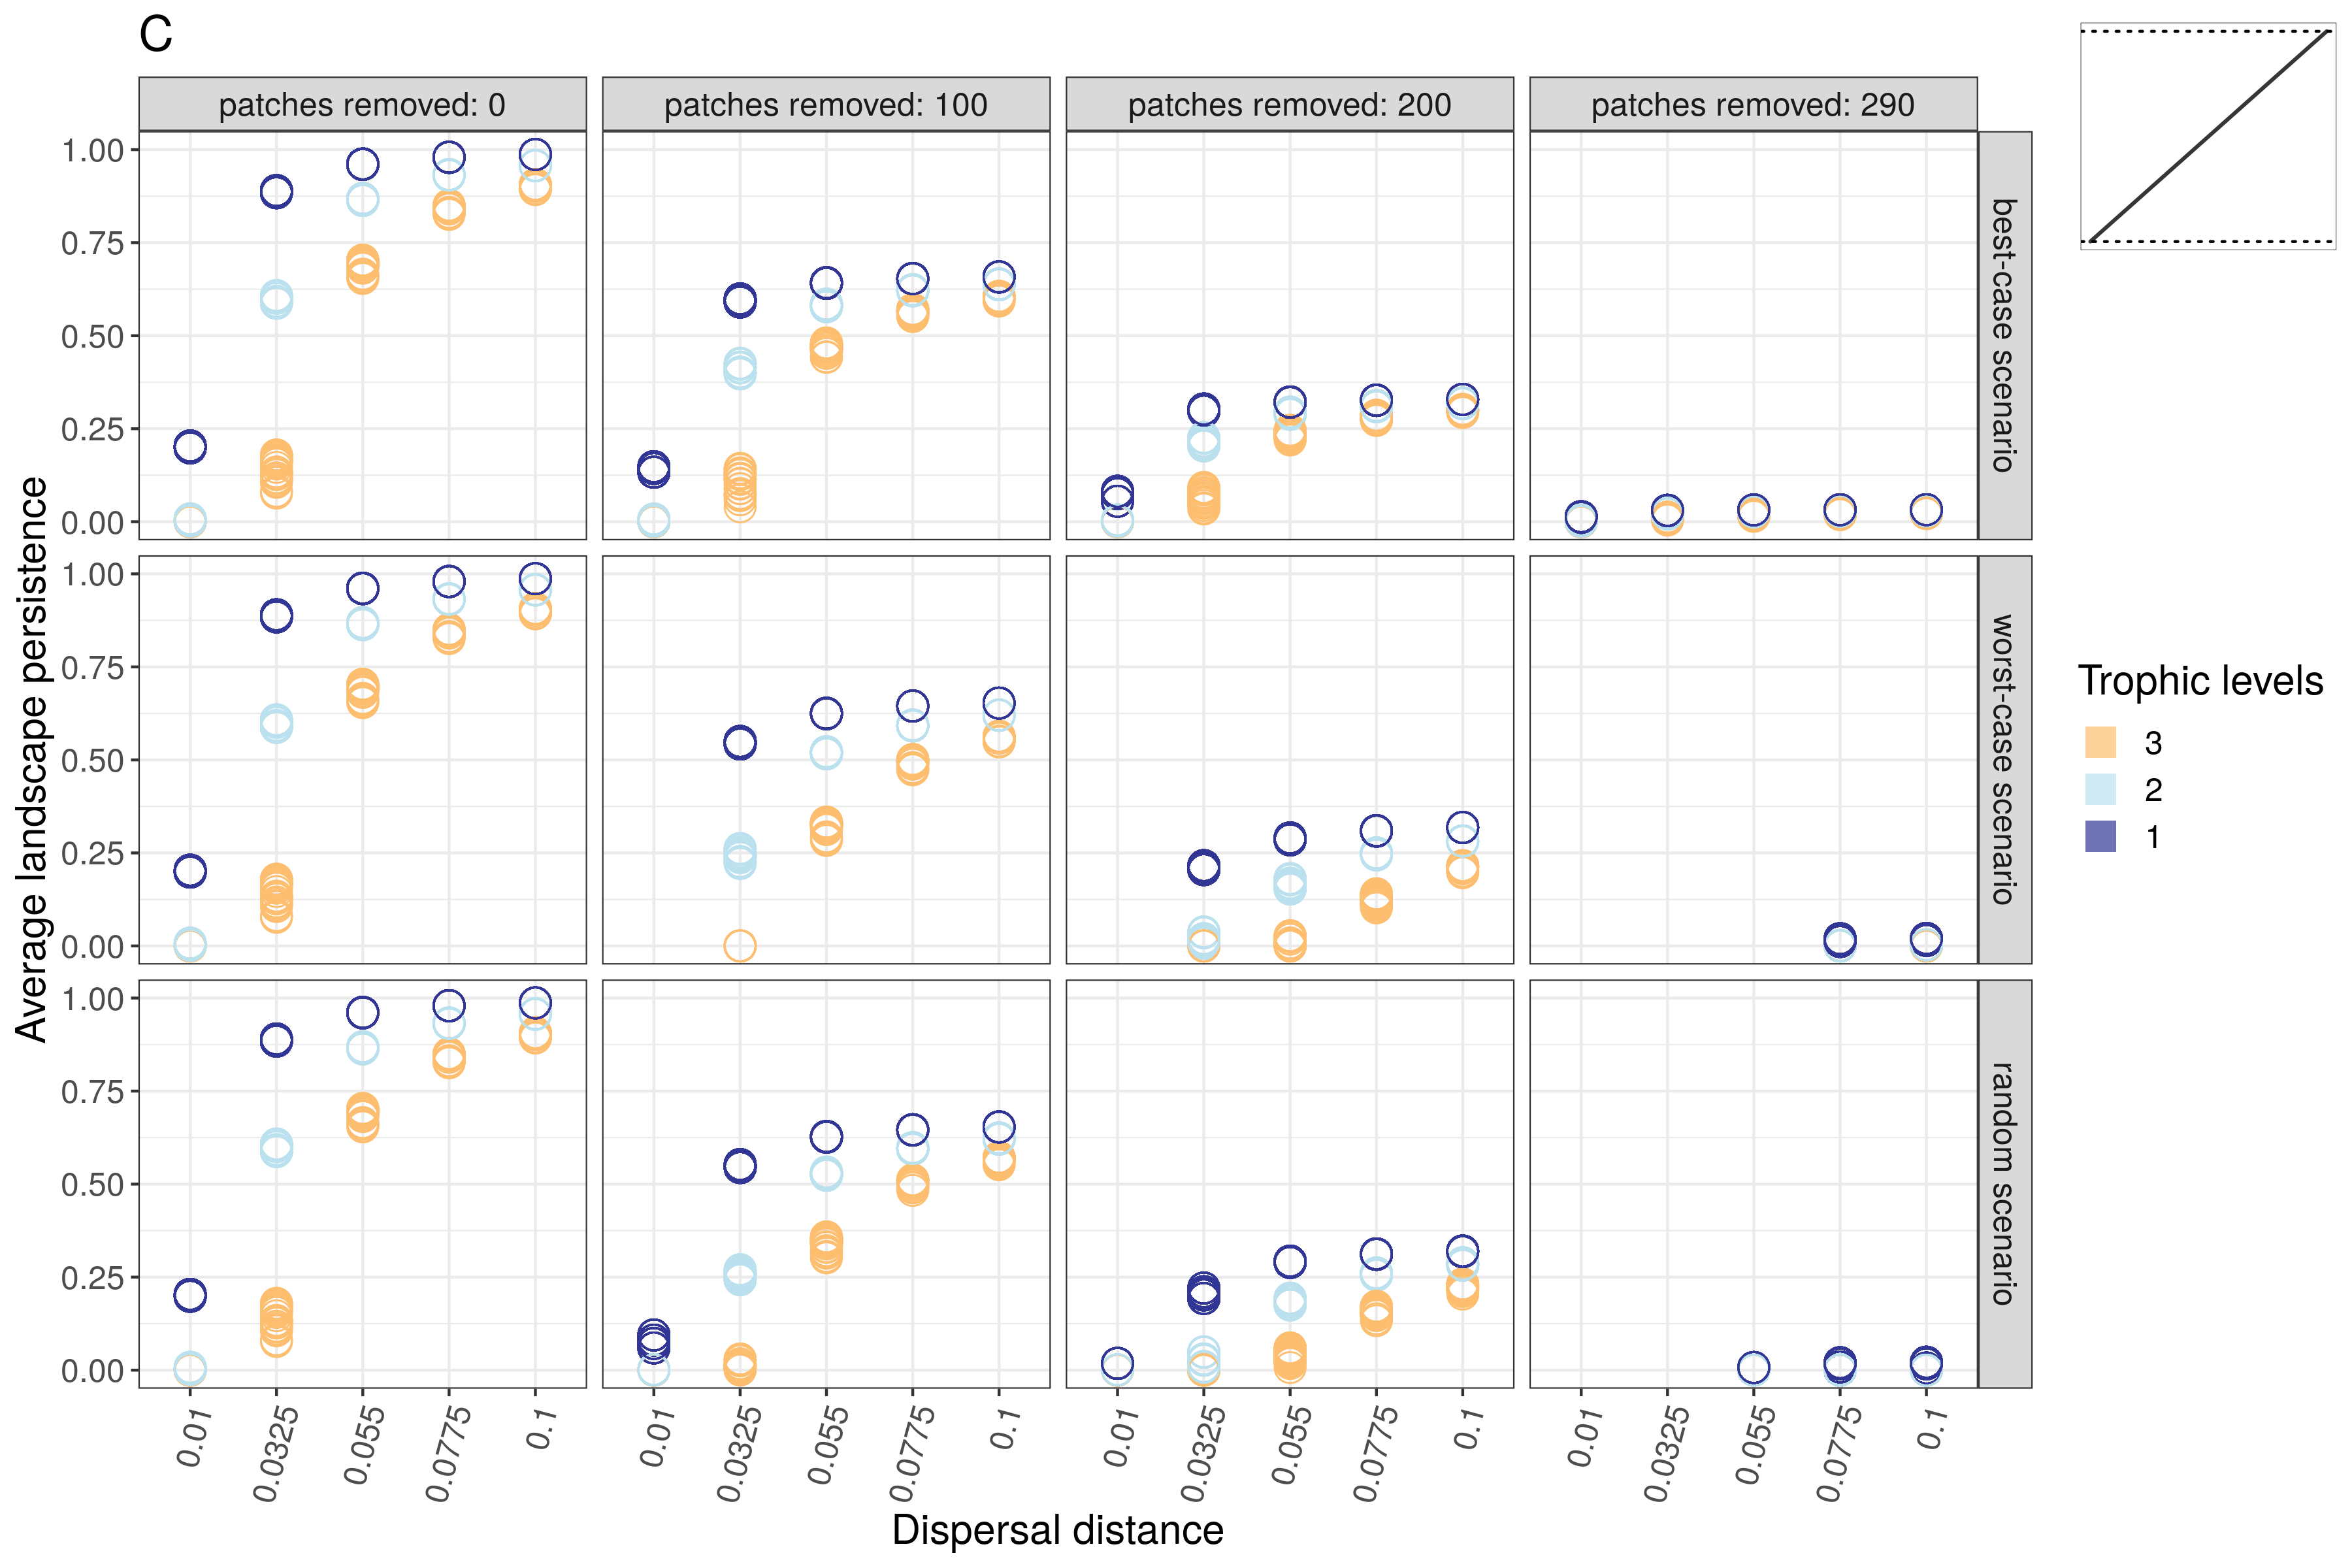
\includegraphics[width=0.8\textwidth,valign=t]{sump_Serengeti_food_web_with_32_consumer_and_129_basal_species_basal_1_1.png}
  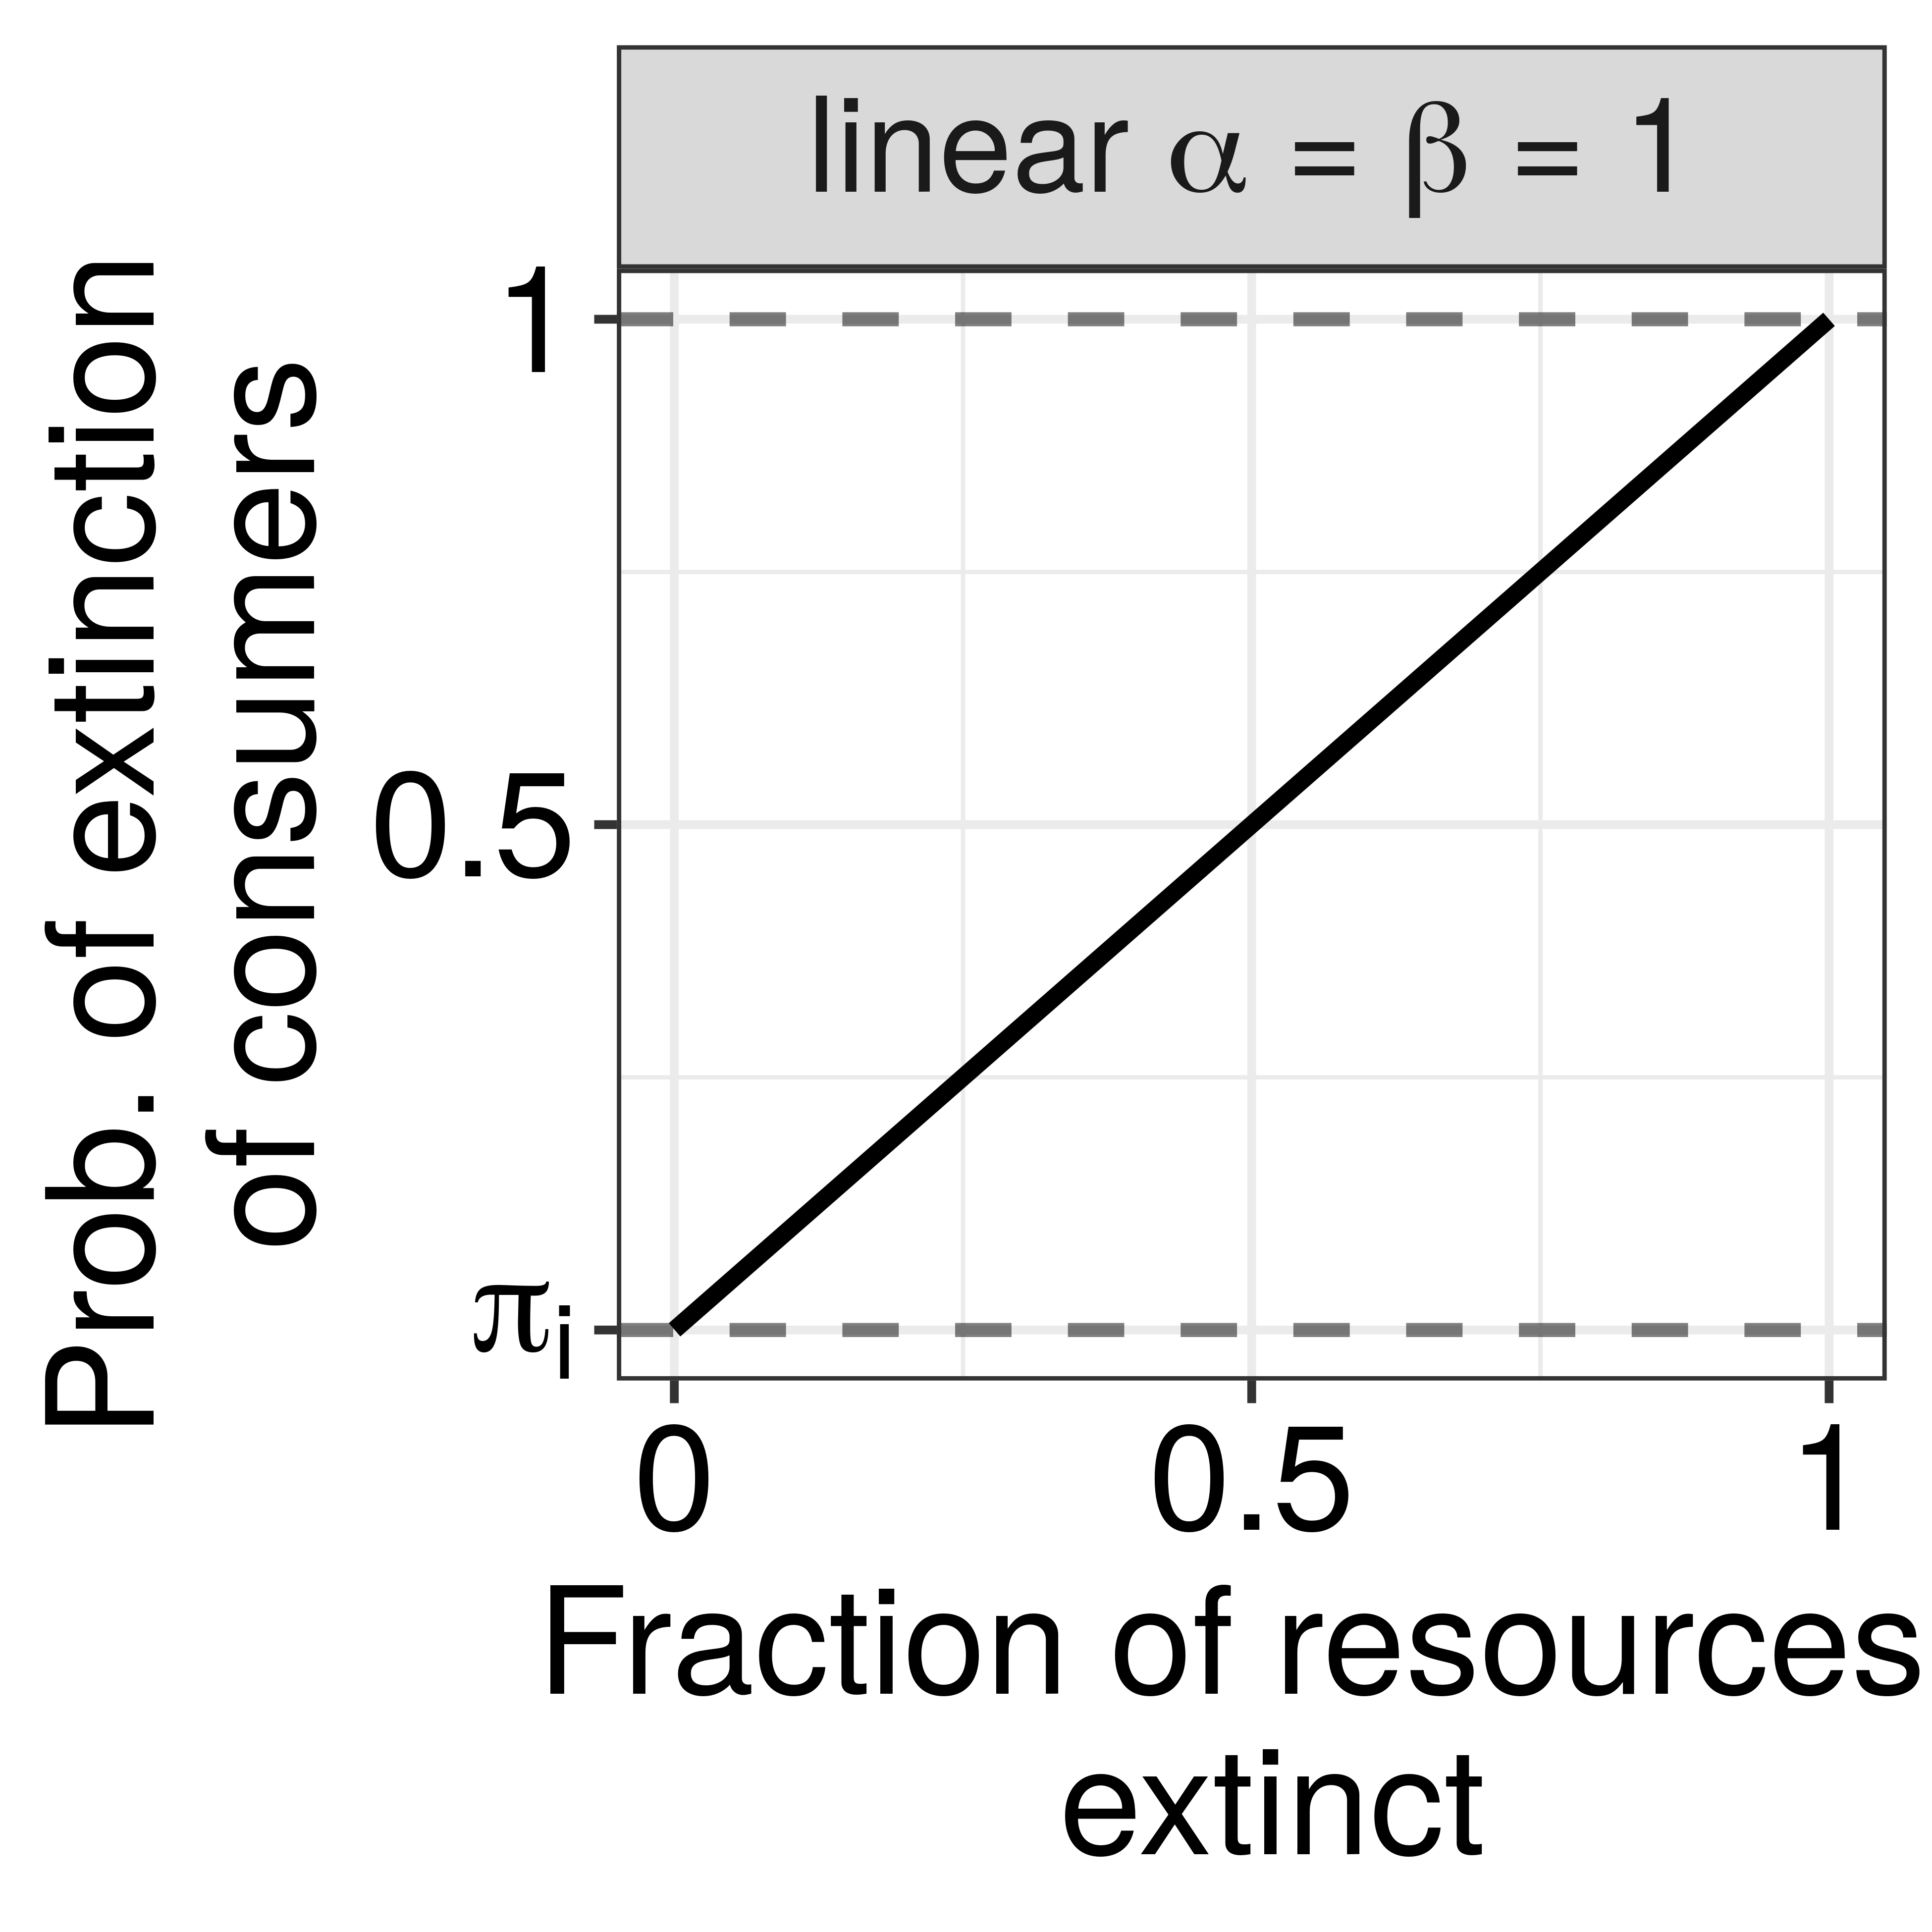
\includegraphics[width=0.19\textwidth,valign=t]{fform_1_1.png}
  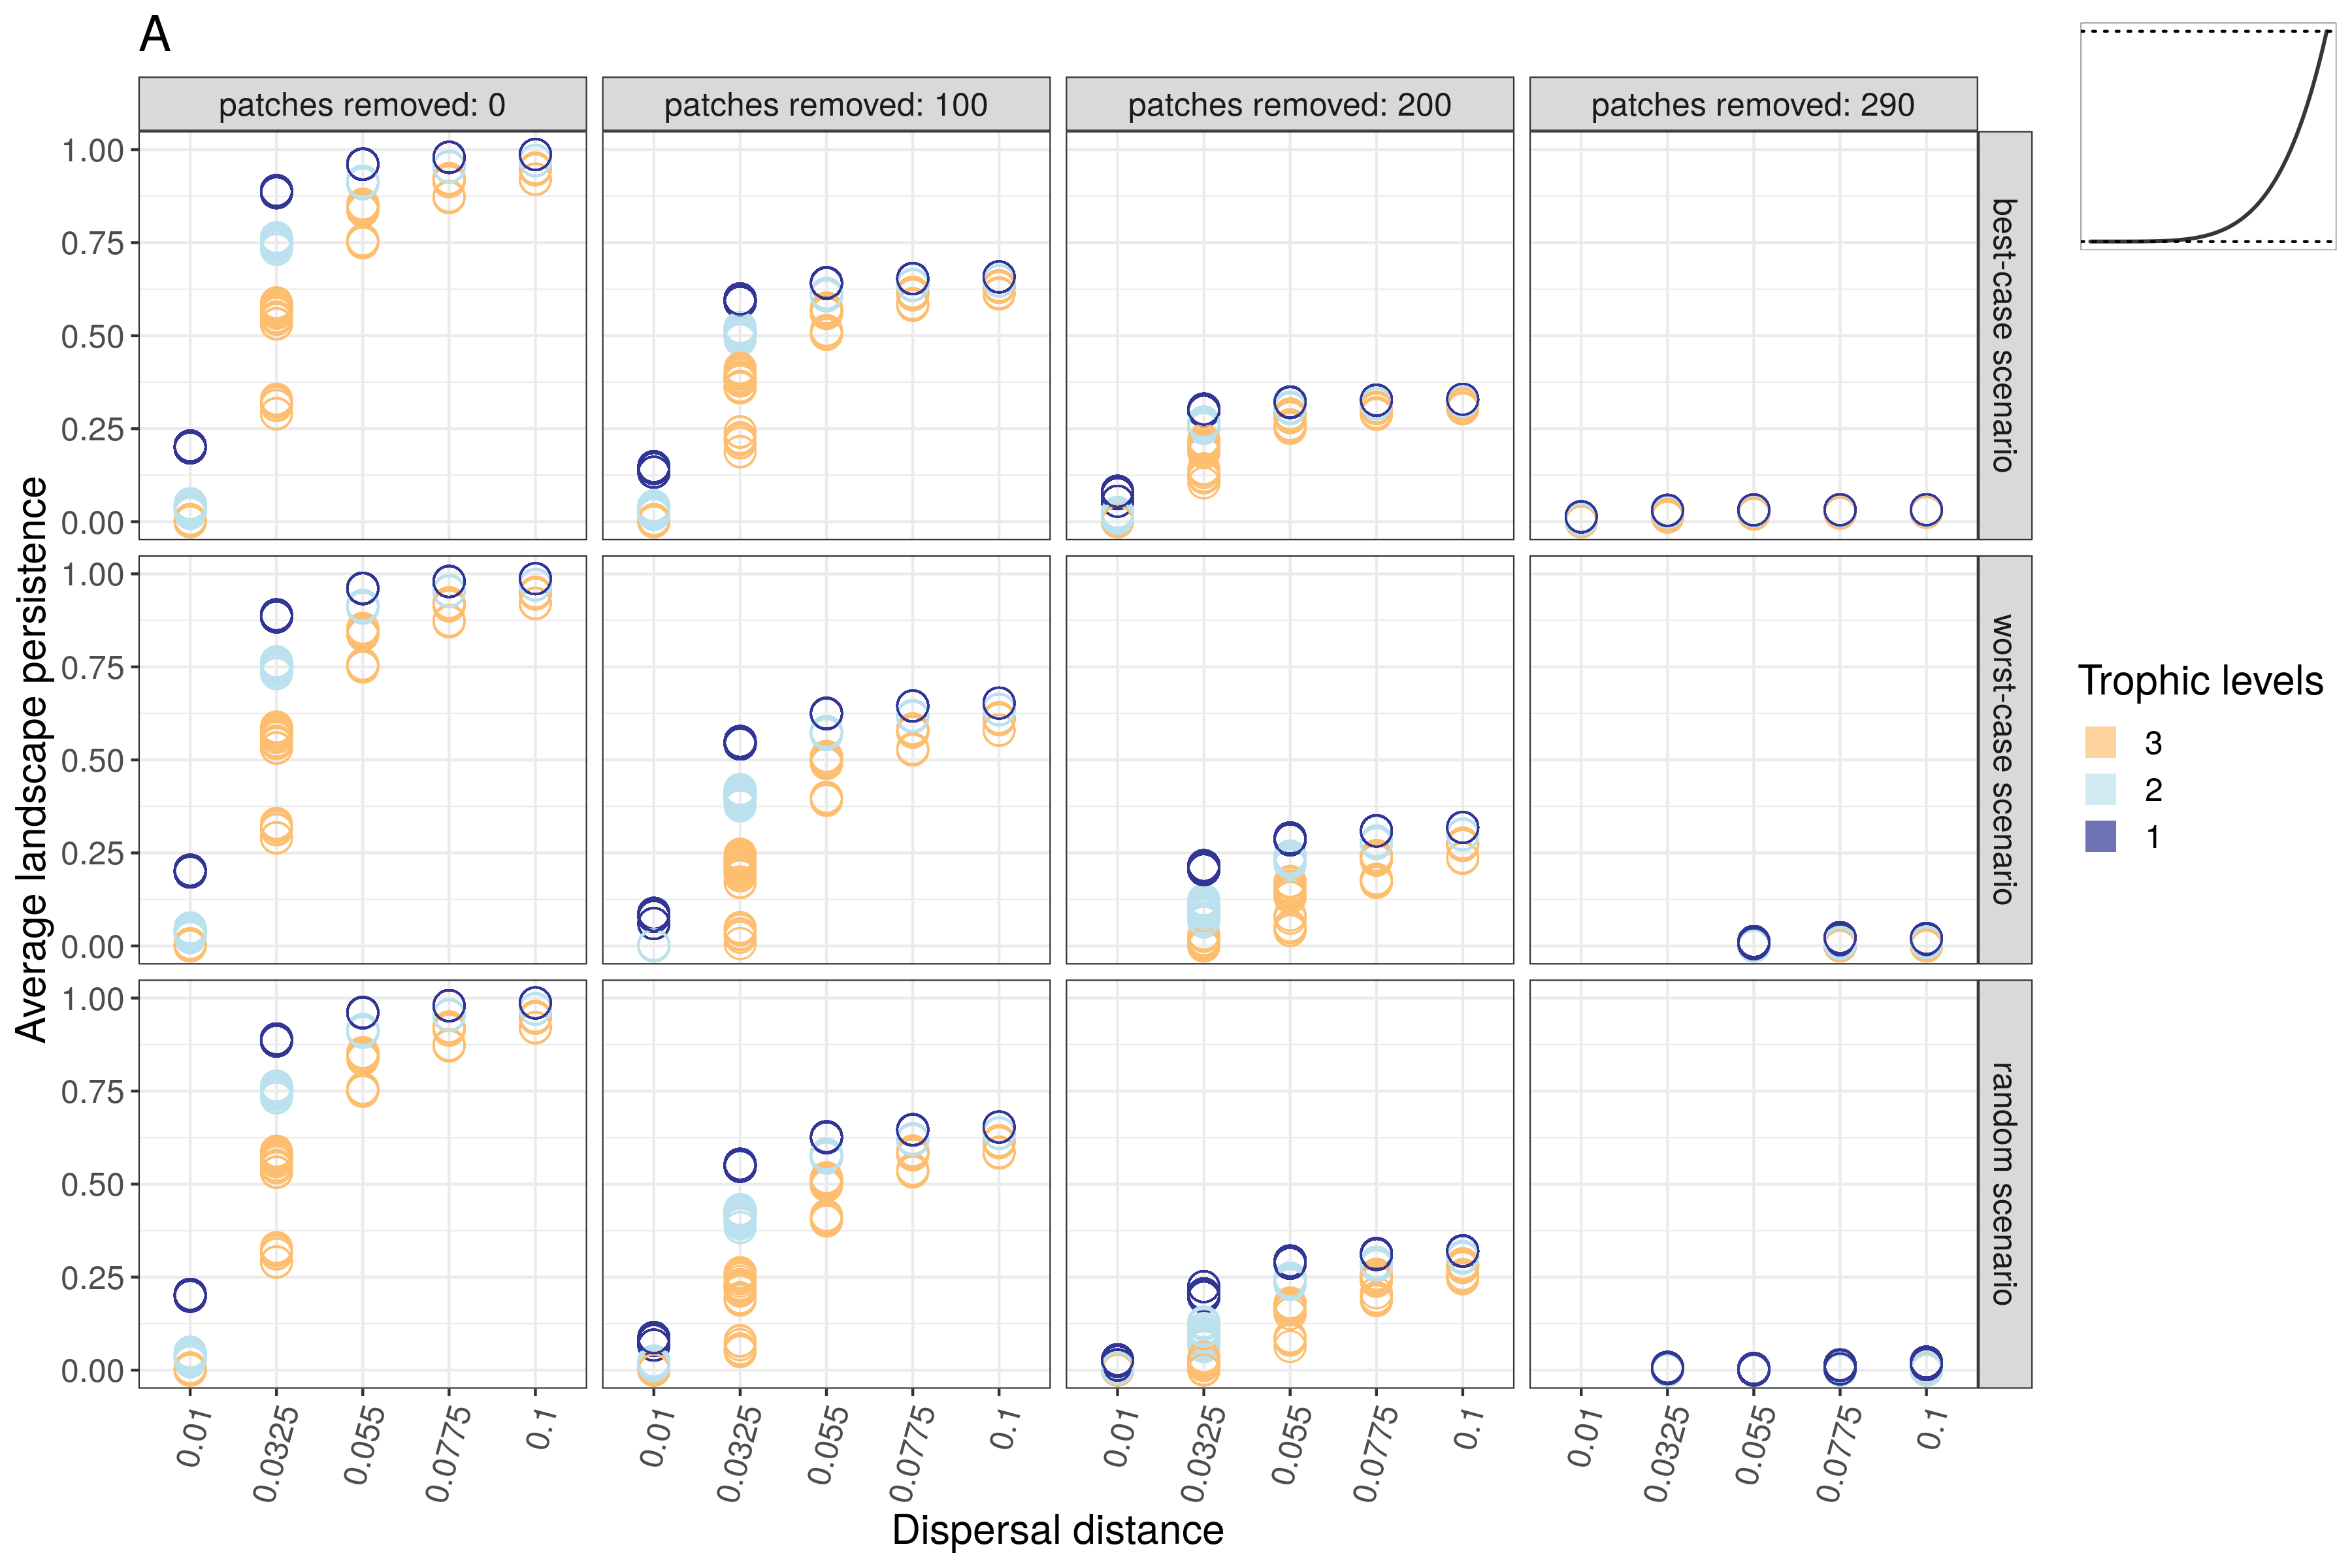
\includegraphics[width=0.8\textwidth,valign=t]{sump_Serengeti_food_web_with_32_consumer_and_129_basal_species_basal_5_1.png}
    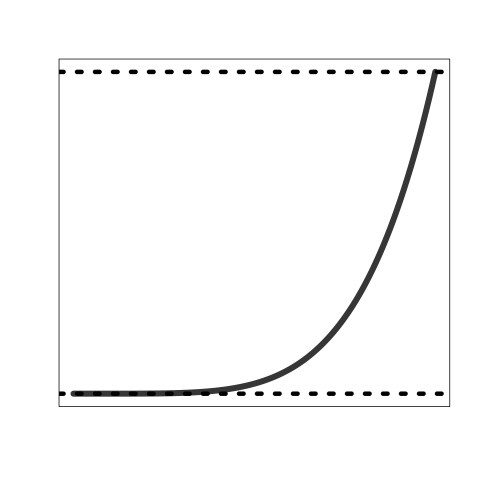
\includegraphics[width=0.19\textwidth,valign=t]{fform_5_1.png}
\caption{As Figure \ref{S_fig:patchloss_300_100_distance_1}, but for the Serengeti food web.}
\label{S_fig:patchloss_Serengeti_TLB_distance_1}
\end{figure}

\begin{figure}\ContinuedFloat
  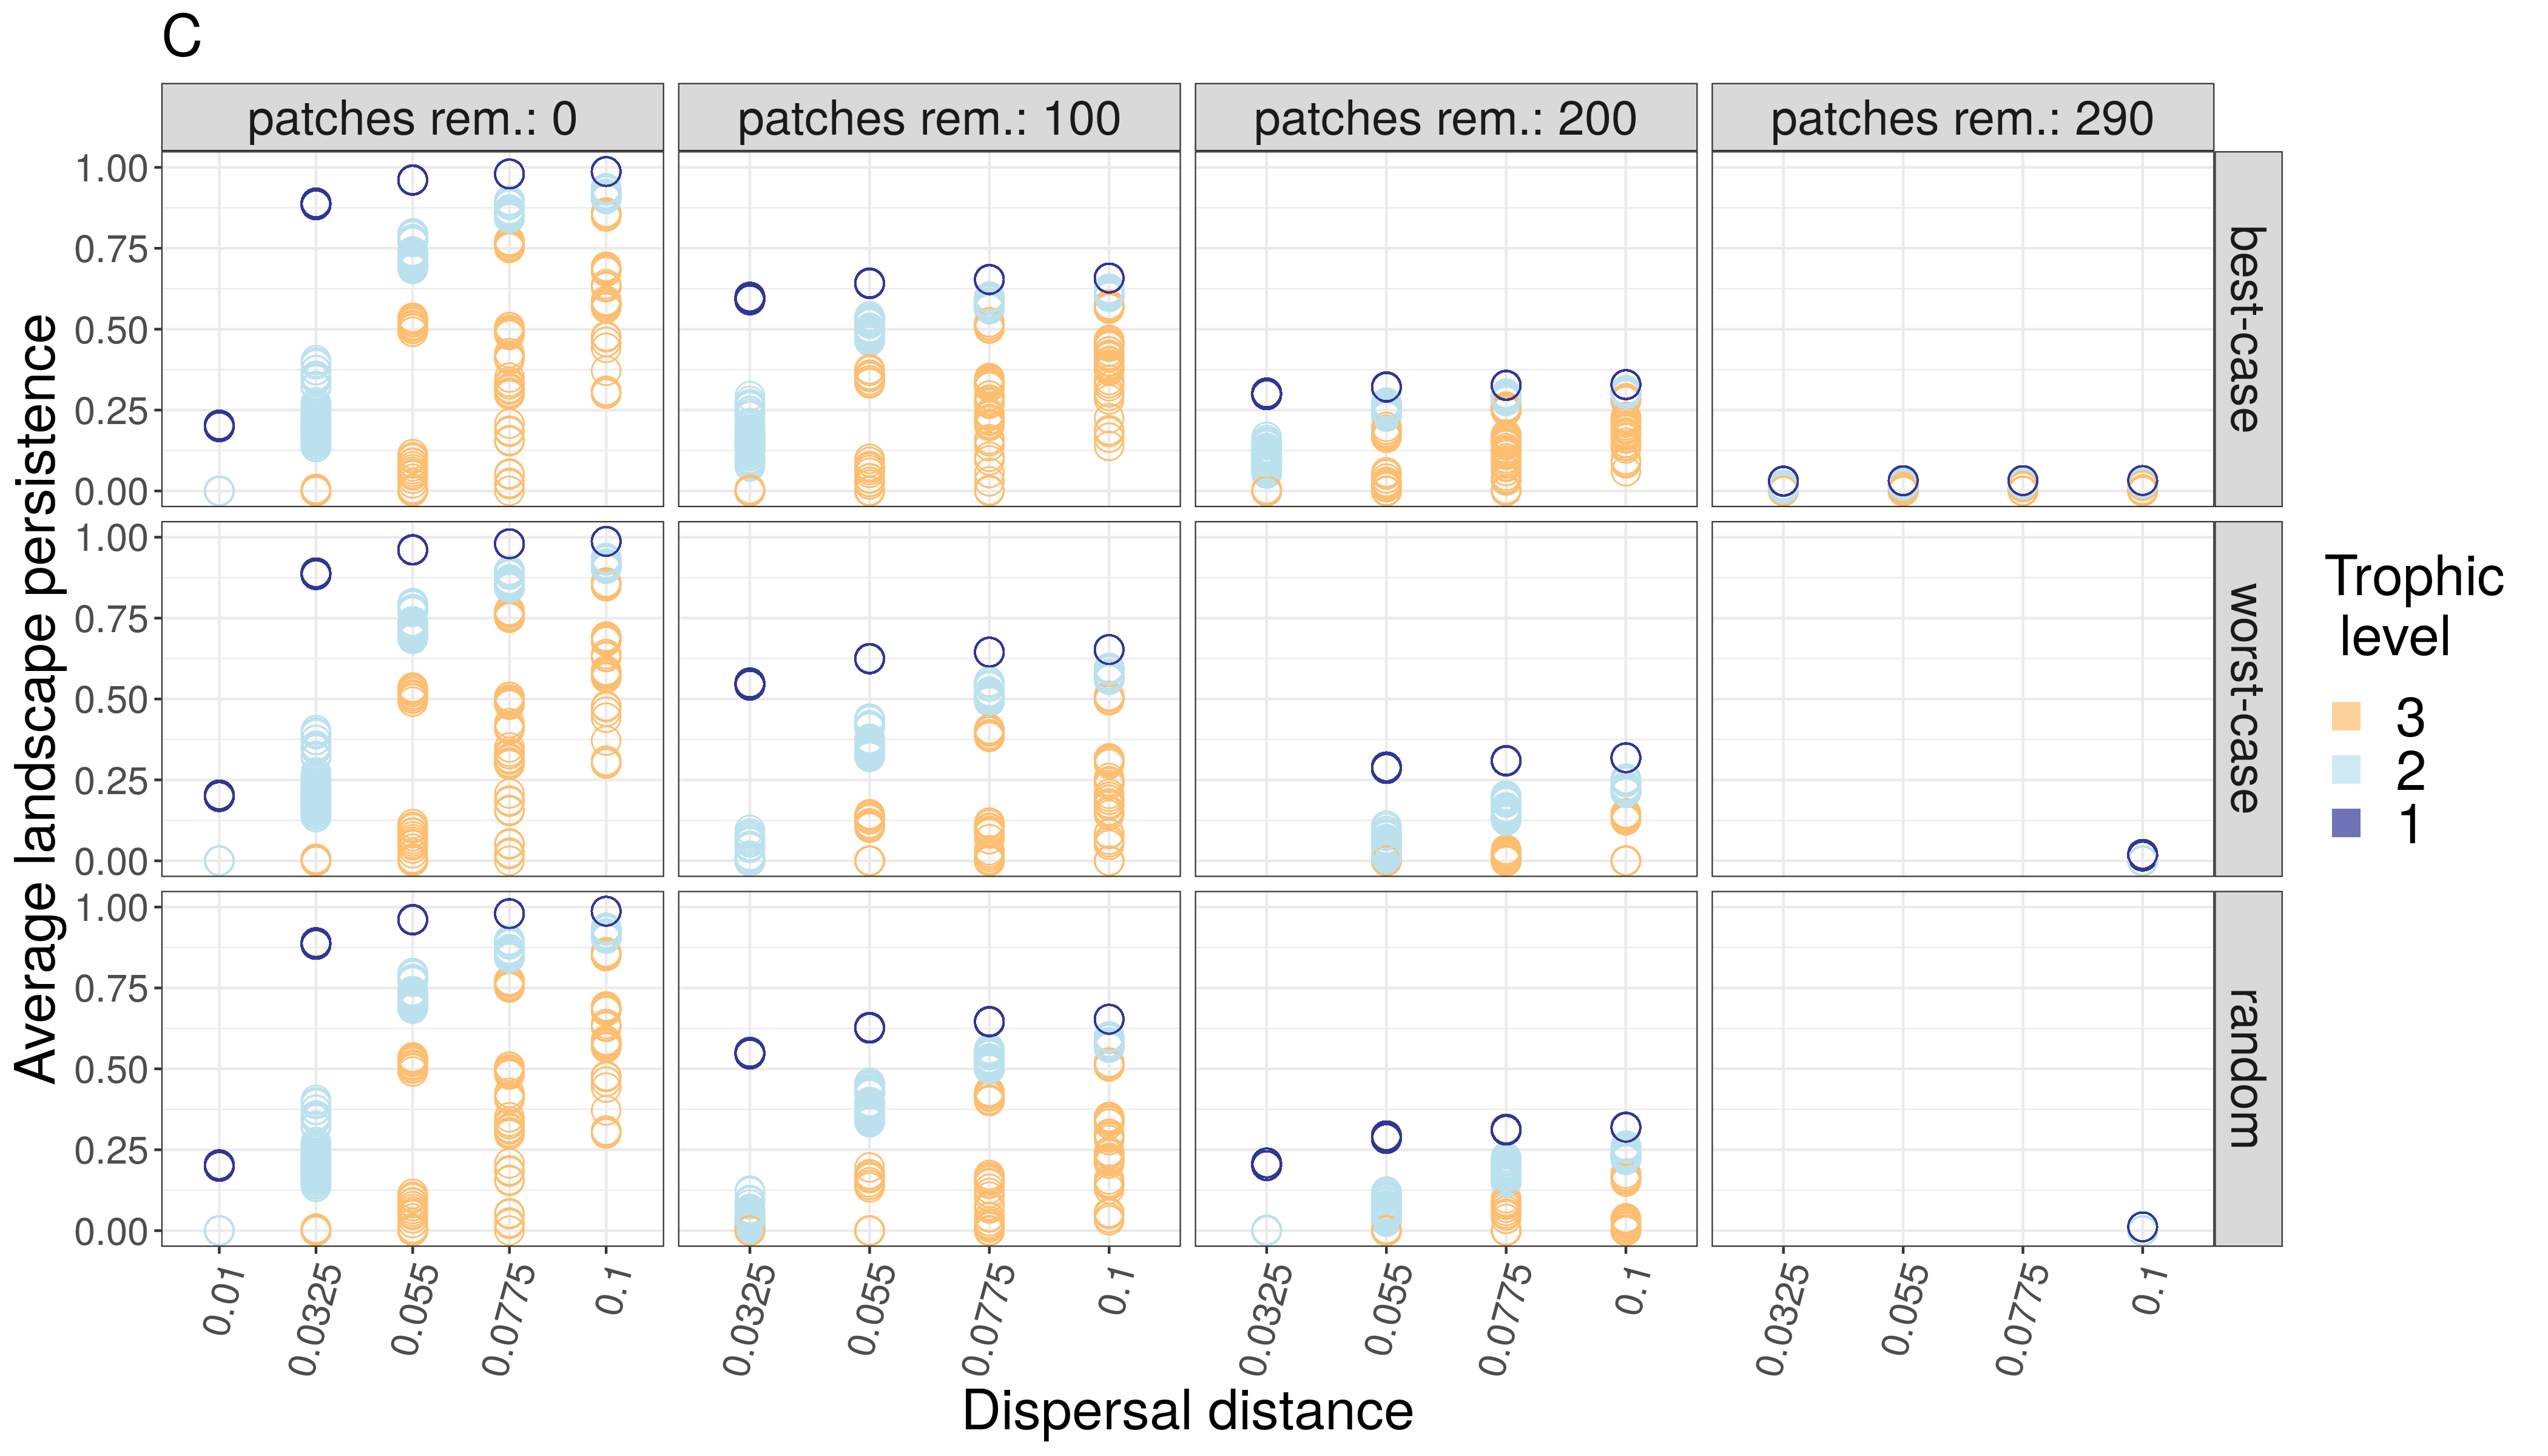
\includegraphics[width=0.8\textwidth,valign=t]{sump_Serengeti_food_web_with_32_consumer_and_129_basal_species_basal_1_5.png}
  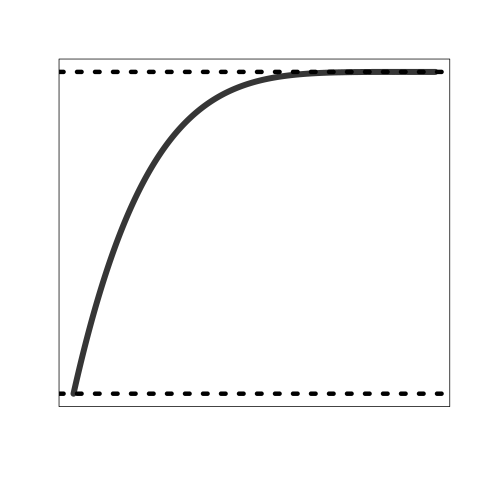
\includegraphics[width=0.19\textwidth,valign=t]{fform_1_5.png}
  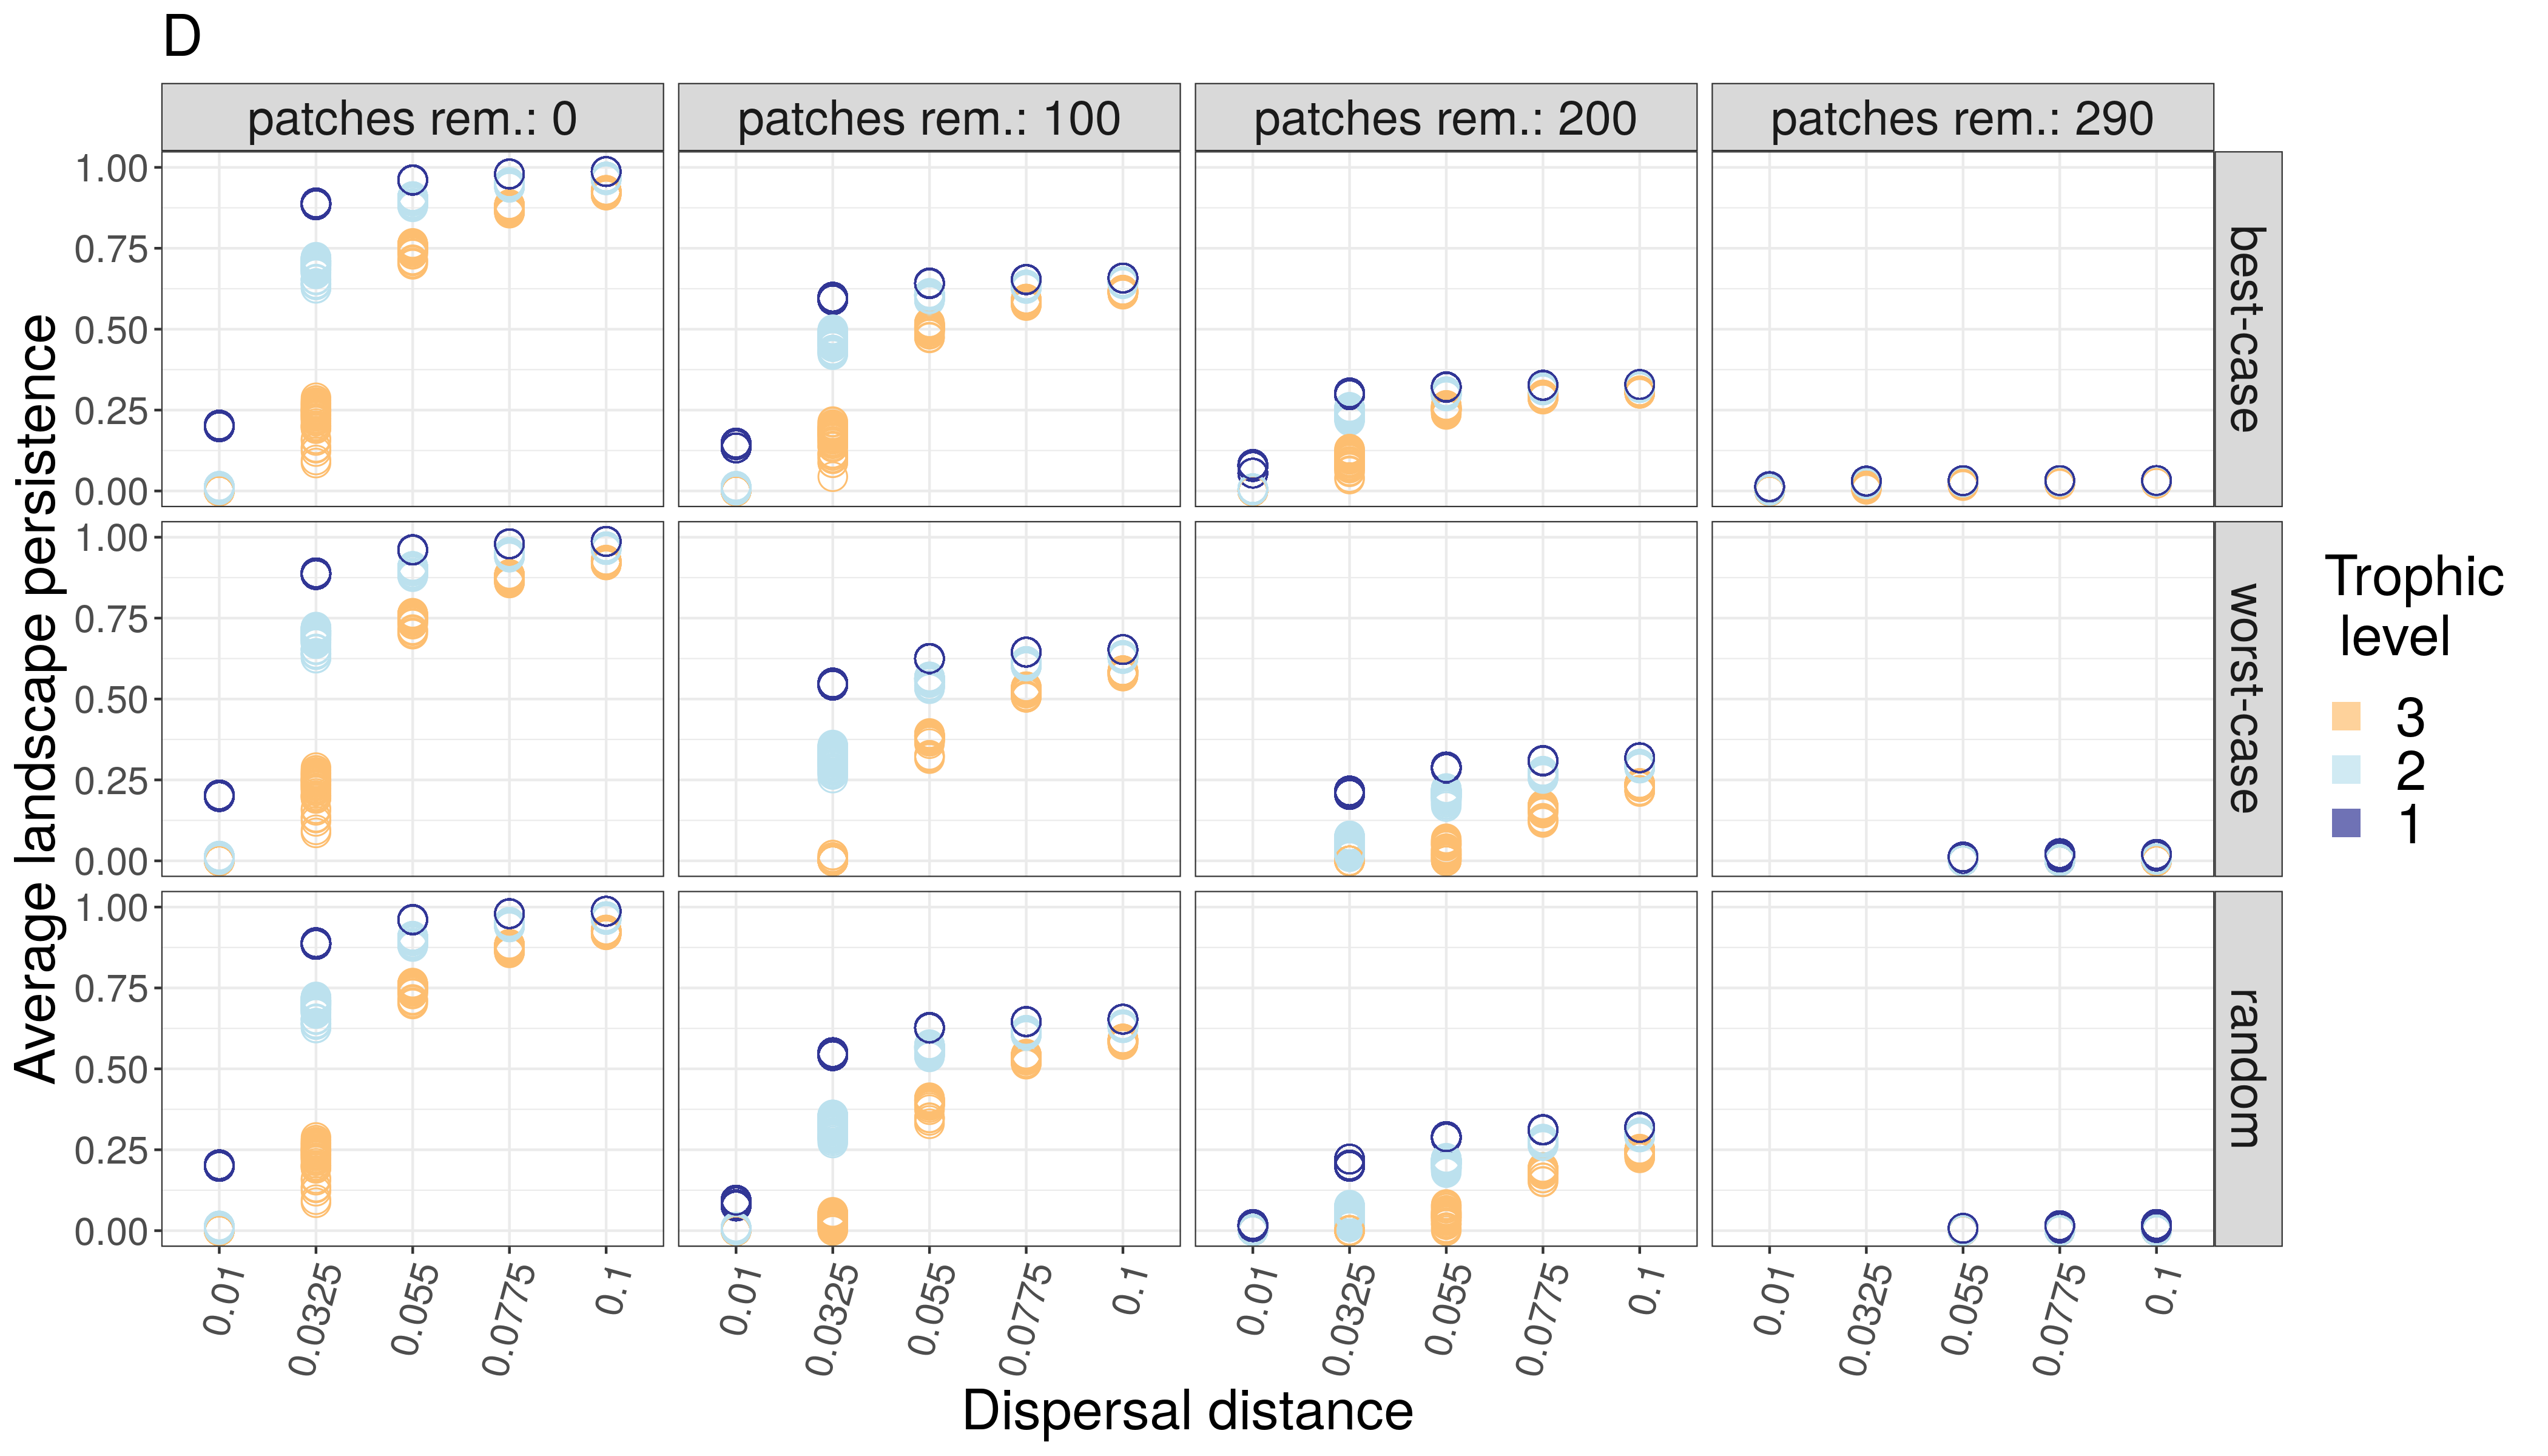
\includegraphics[width=0.8\textwidth,valign=t]{sump_Serengeti_food_web_with_32_consumer_and_129_basal_species_basal_5_5.png}
  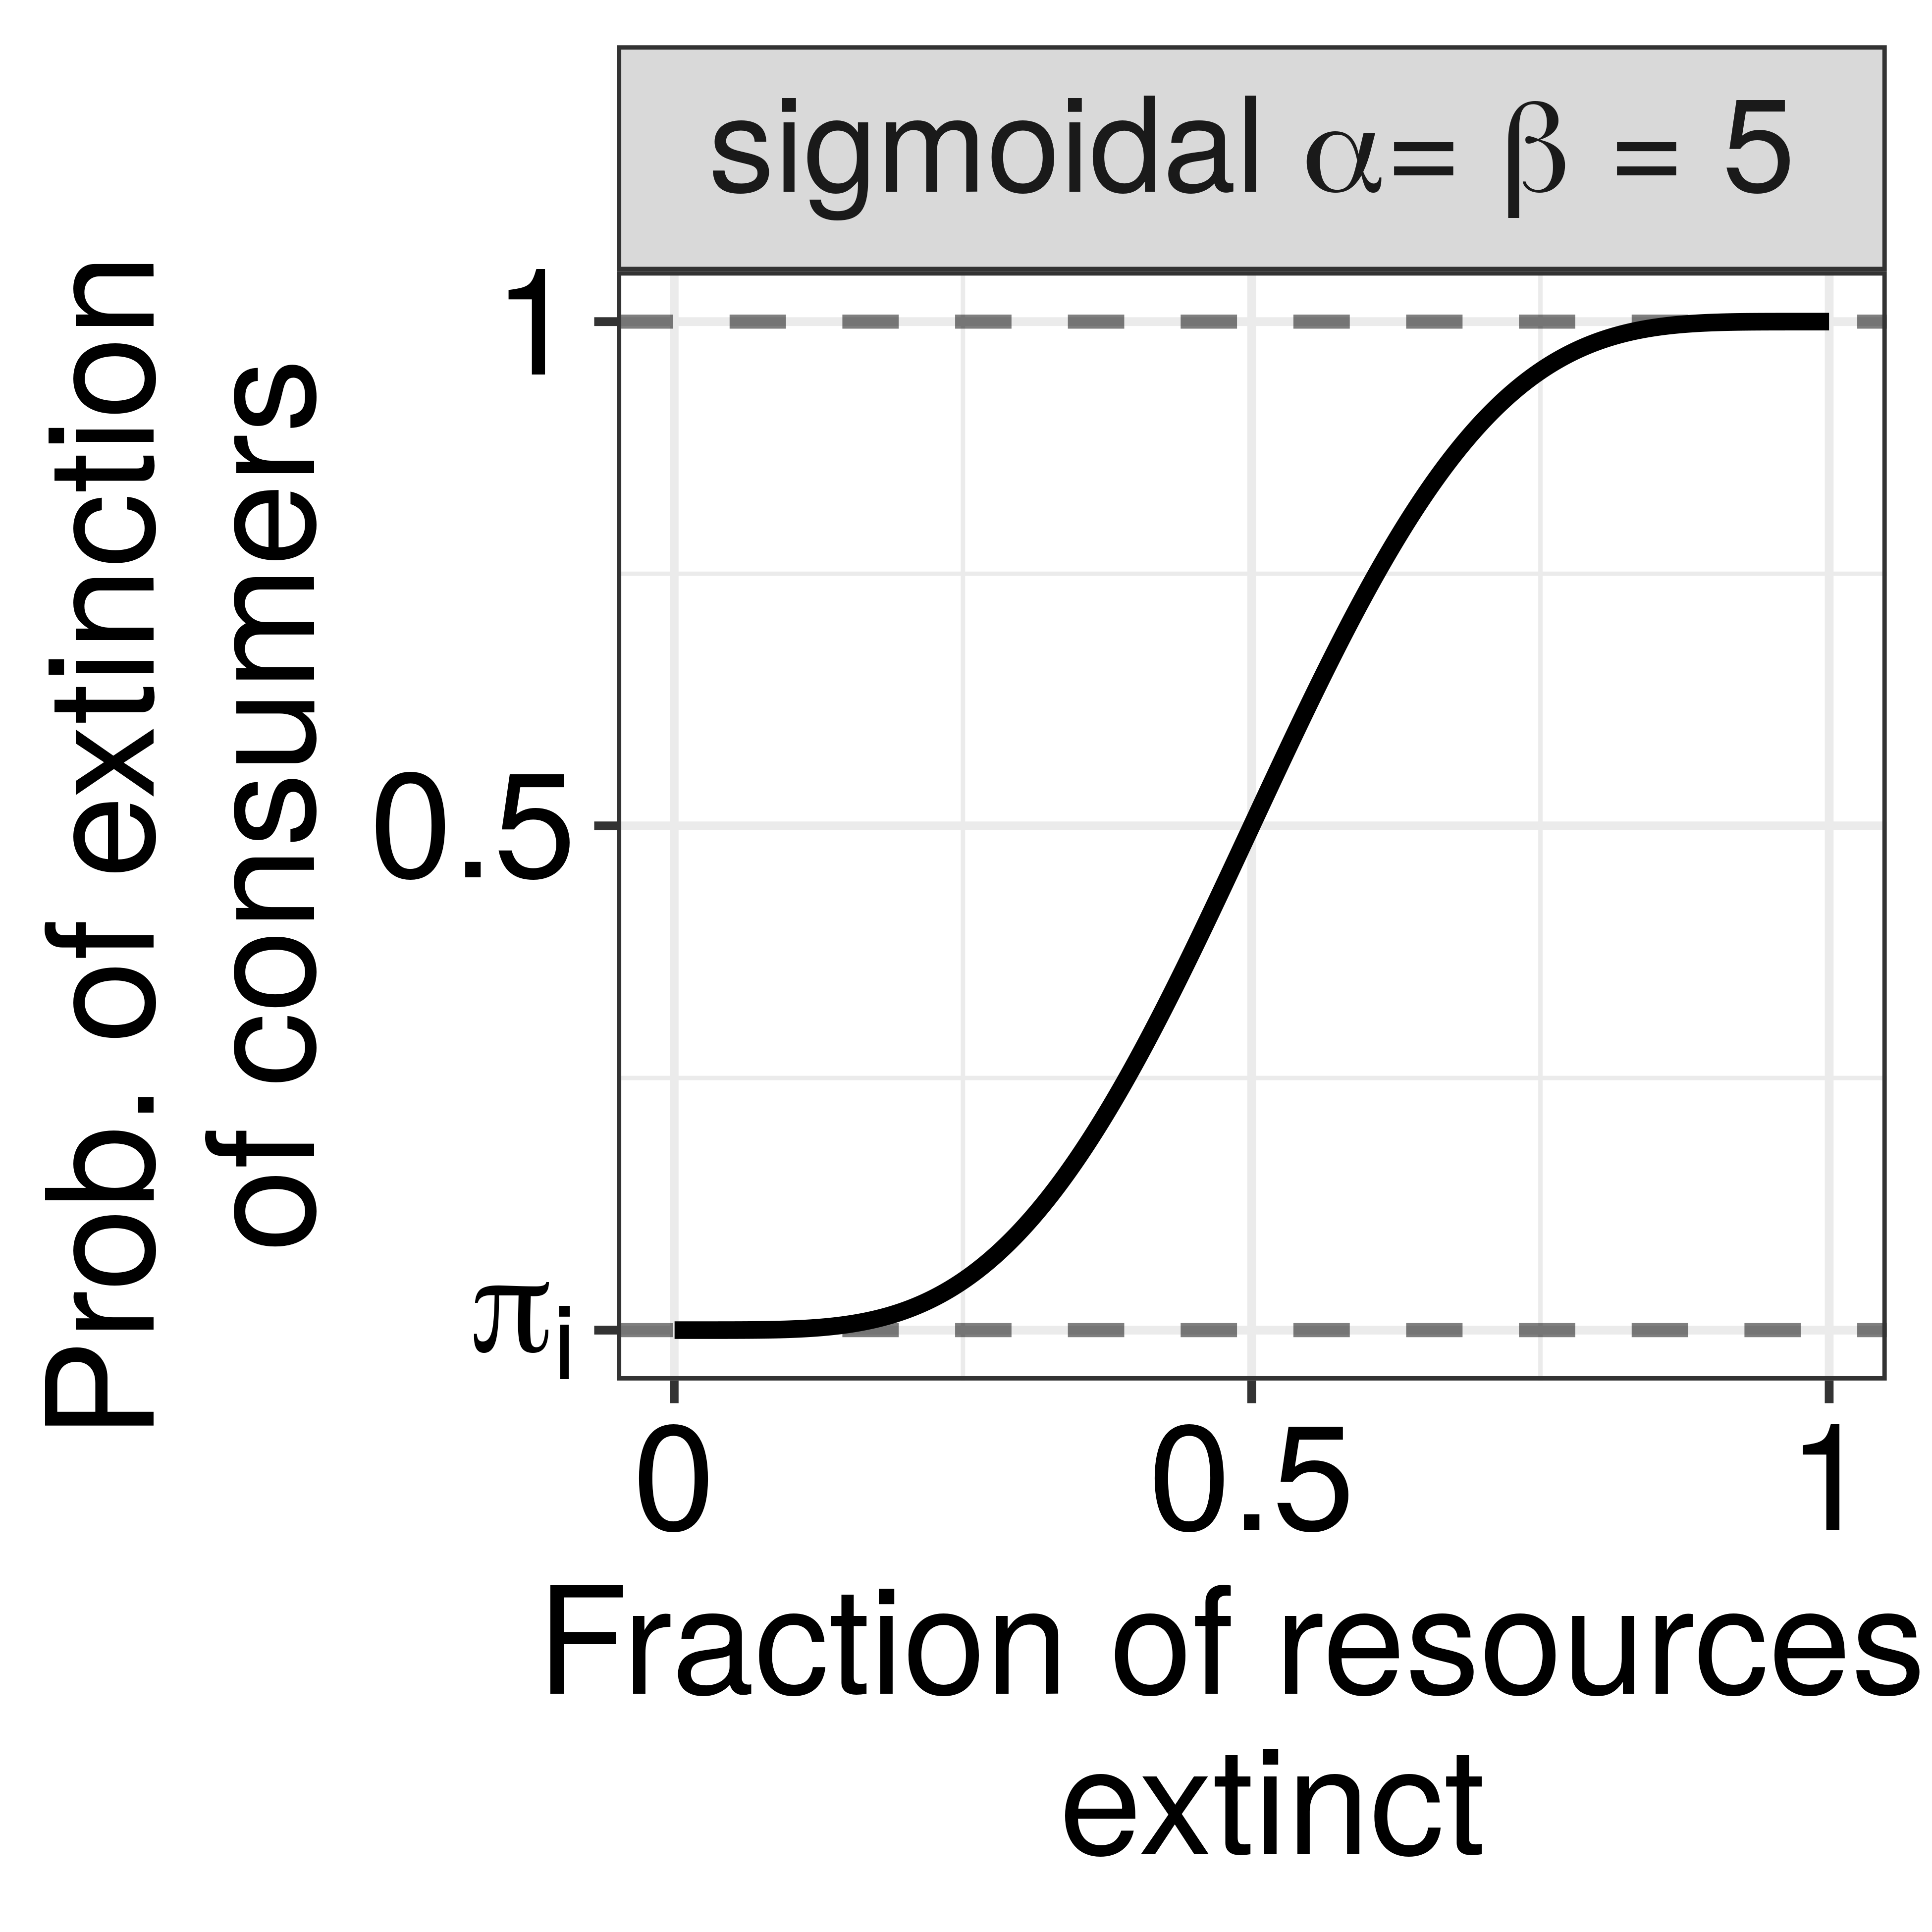
\includegraphics[width=0.19\textwidth,valign=t]{fform_5_5.png}
\caption{Figure continued.}
\label{S_fig:patchloss_Serengeti_TLB_distance_2}
\end{figure}

\begin{figure}
\centering
\hspace{-5em}
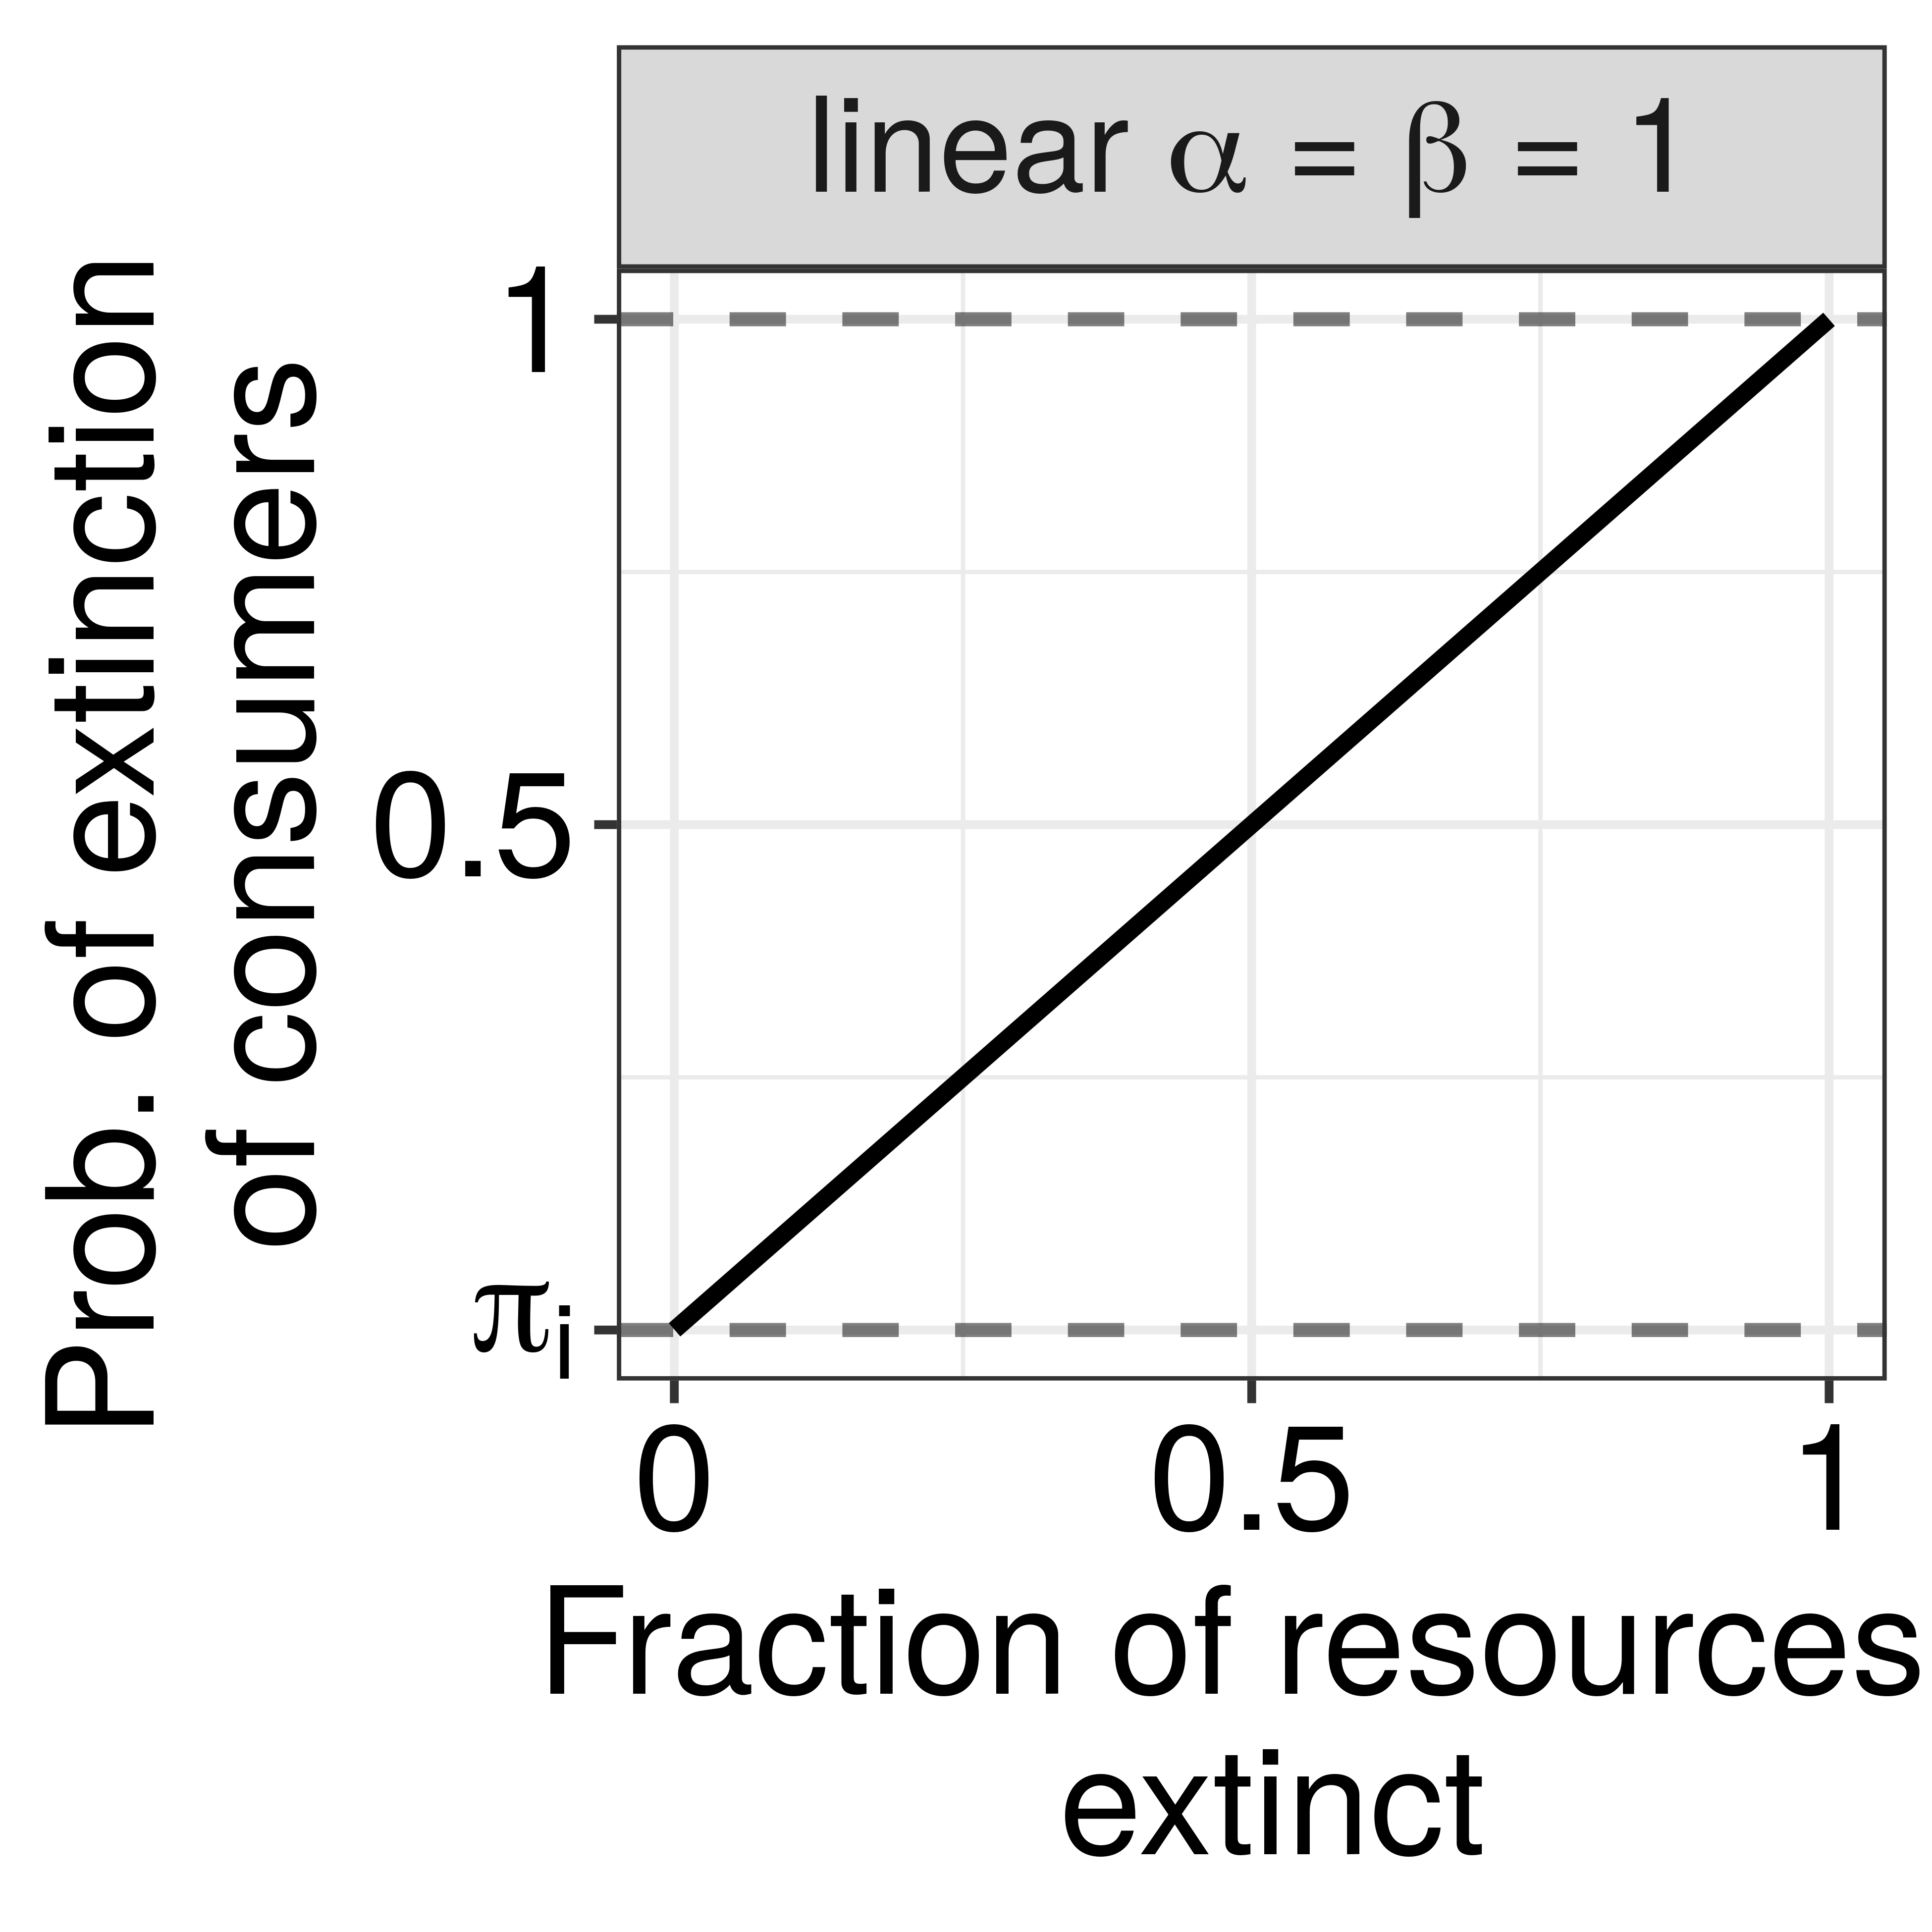
\includegraphics[width=0.2\textwidth]{fform_1_1.png}
\hspace{0.5em}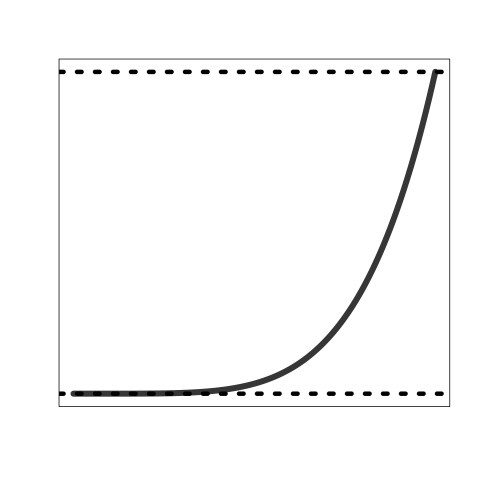
\includegraphics[width=0.2\textwidth]{fform_5_1.png}
\hspace{0.5em}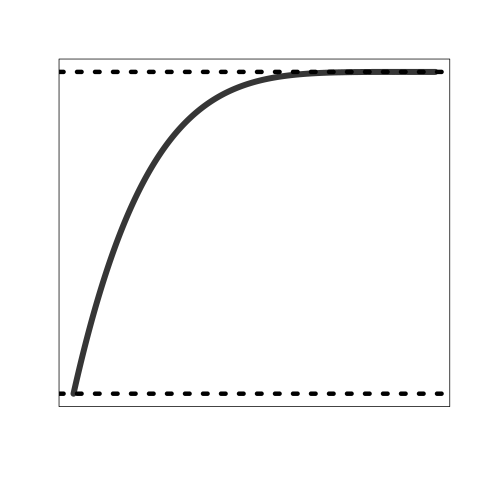
\includegraphics[width=0.2\textwidth]{fform_1_5.png} \hspace{0.5em}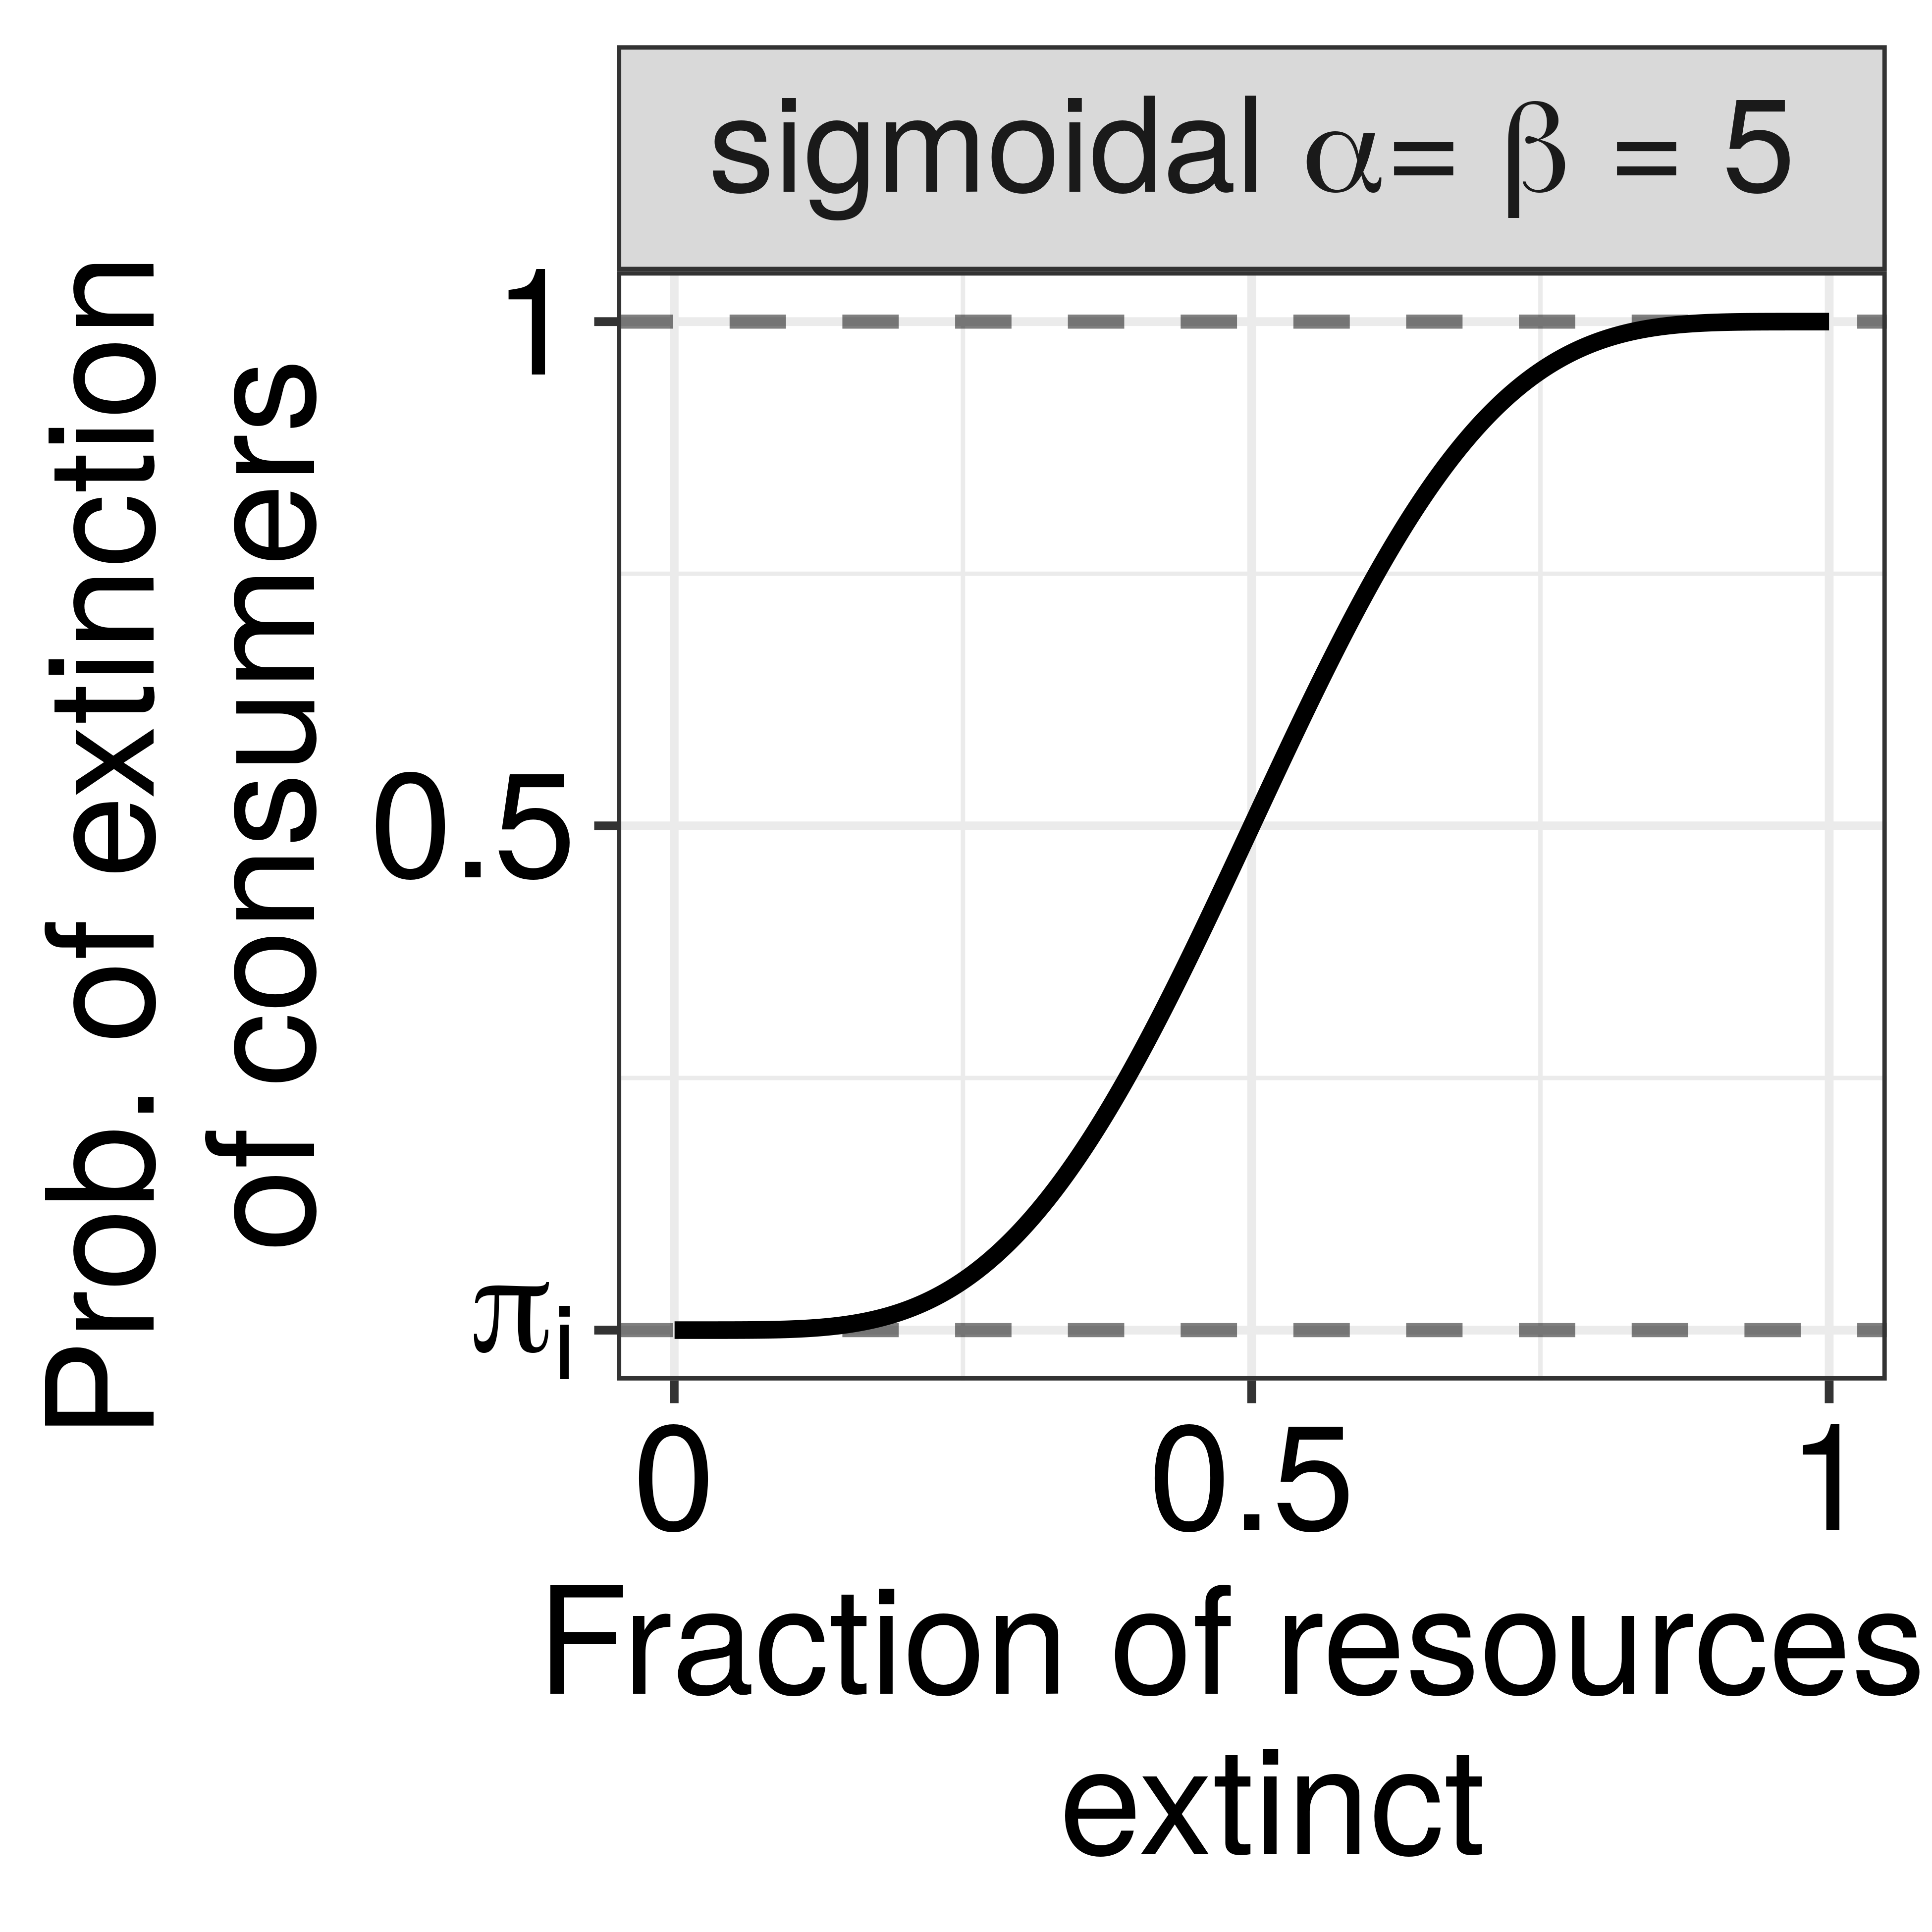
\includegraphics[width=0.2\textwidth]{fform_5_5.png}

\vspace{1.5em} 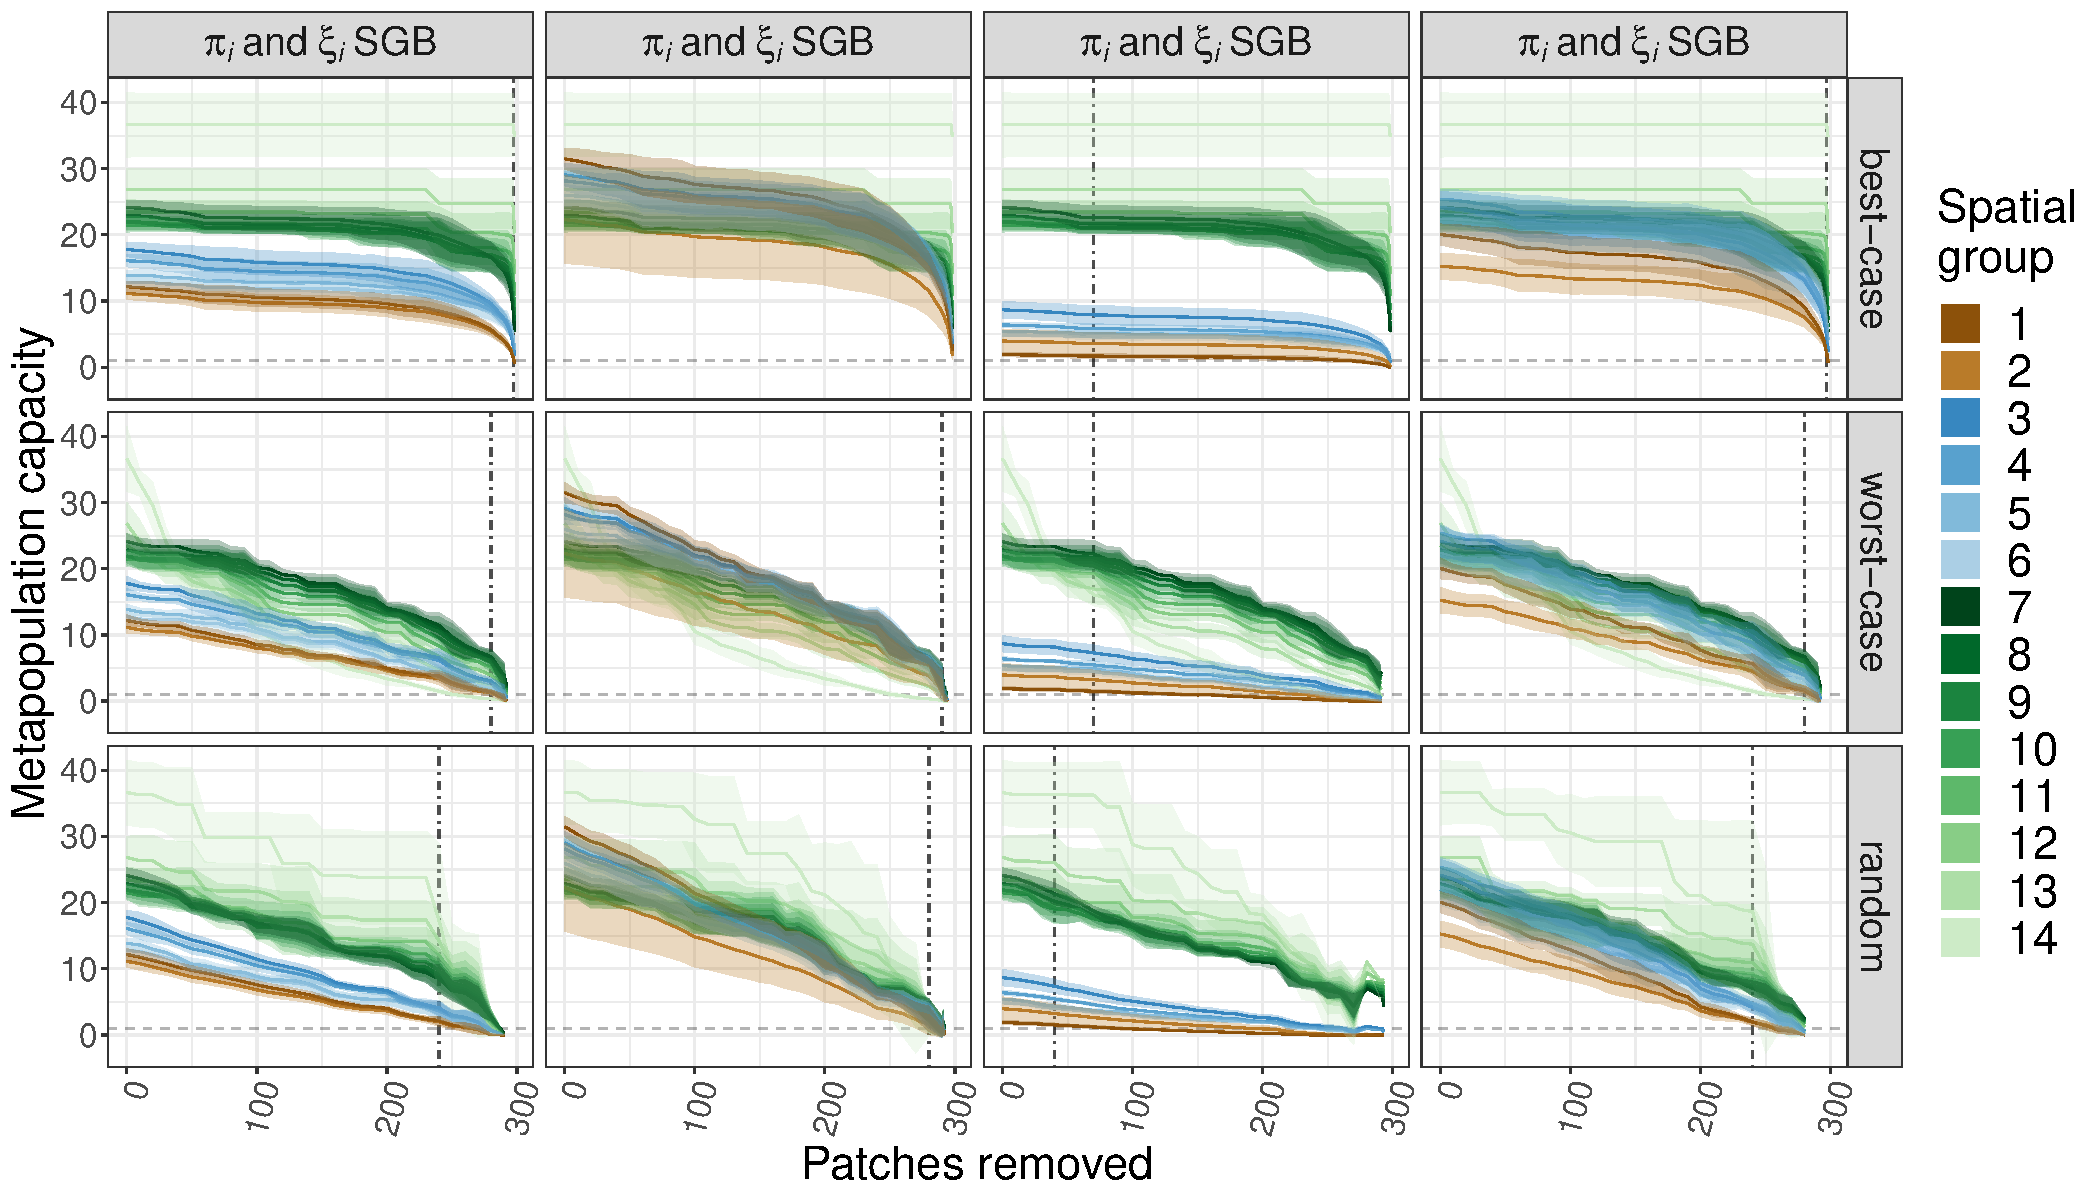
\includegraphics[width=\textwidth]{lambda_Serengeti_food_web_with_32_consumer_and_129_basal_species_basal_SGB_BOSAUG.pdf}
\caption{As Figure~4 in the main text, except the species whose metapopulation capacity serves as the basis of patch removal is different. In the main text, this species was the Gum arabic tree (\textit{Acacia senegal}), the sole representative of spatial group 12. Here, we have instead chosen a species from spatial group 14, \textit{Boscia augustifolia}. Results are qualitatively unchanged by this alteration.}
\label{S_fig:patchloss_Serengeti_SGB_alt}
\end{figure}


\clearpage

\subsection{Removing patches based on the patch value rankings of top species} \label{sec:tsfs}

For the linear functional form of a consumer's response to the loss of resources, we additionally looked at removing patches based on the patch value rankings of top species, instead of basal ones. This means that patch removal was stopped whenever the top species have gone extinct. In case of the Serengeti food web, we removed patches based on the patch value rankings of the leopard (\textit{Panthera pardus}). 


\begin{figure}[!ht]
\centering  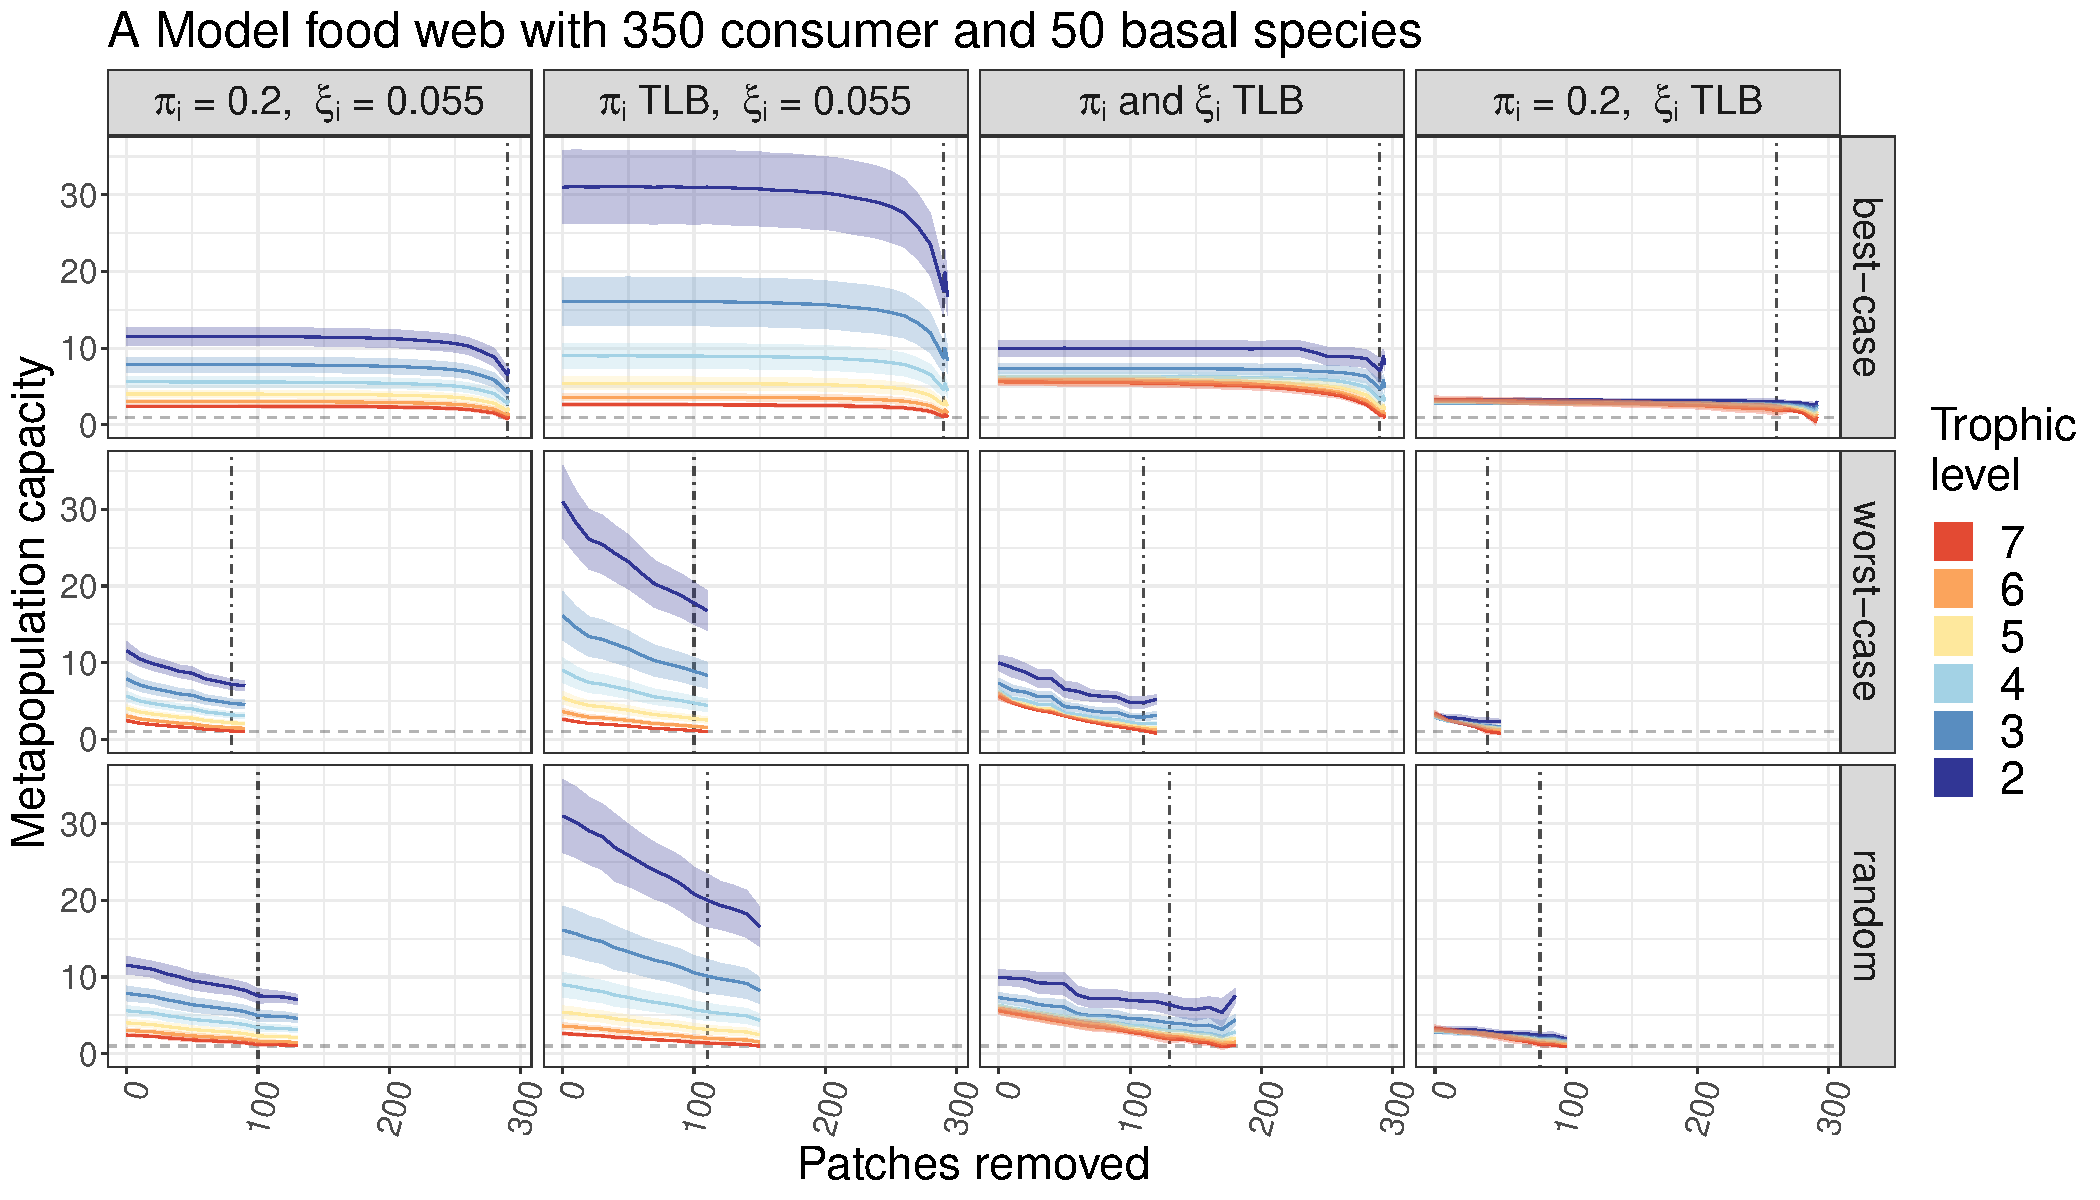
\includegraphics[width=0.8\textwidth,valign=t]{lambda_Model_food_web_with_350_consumer_and_50_basal_species_top_1_1.pdf}
  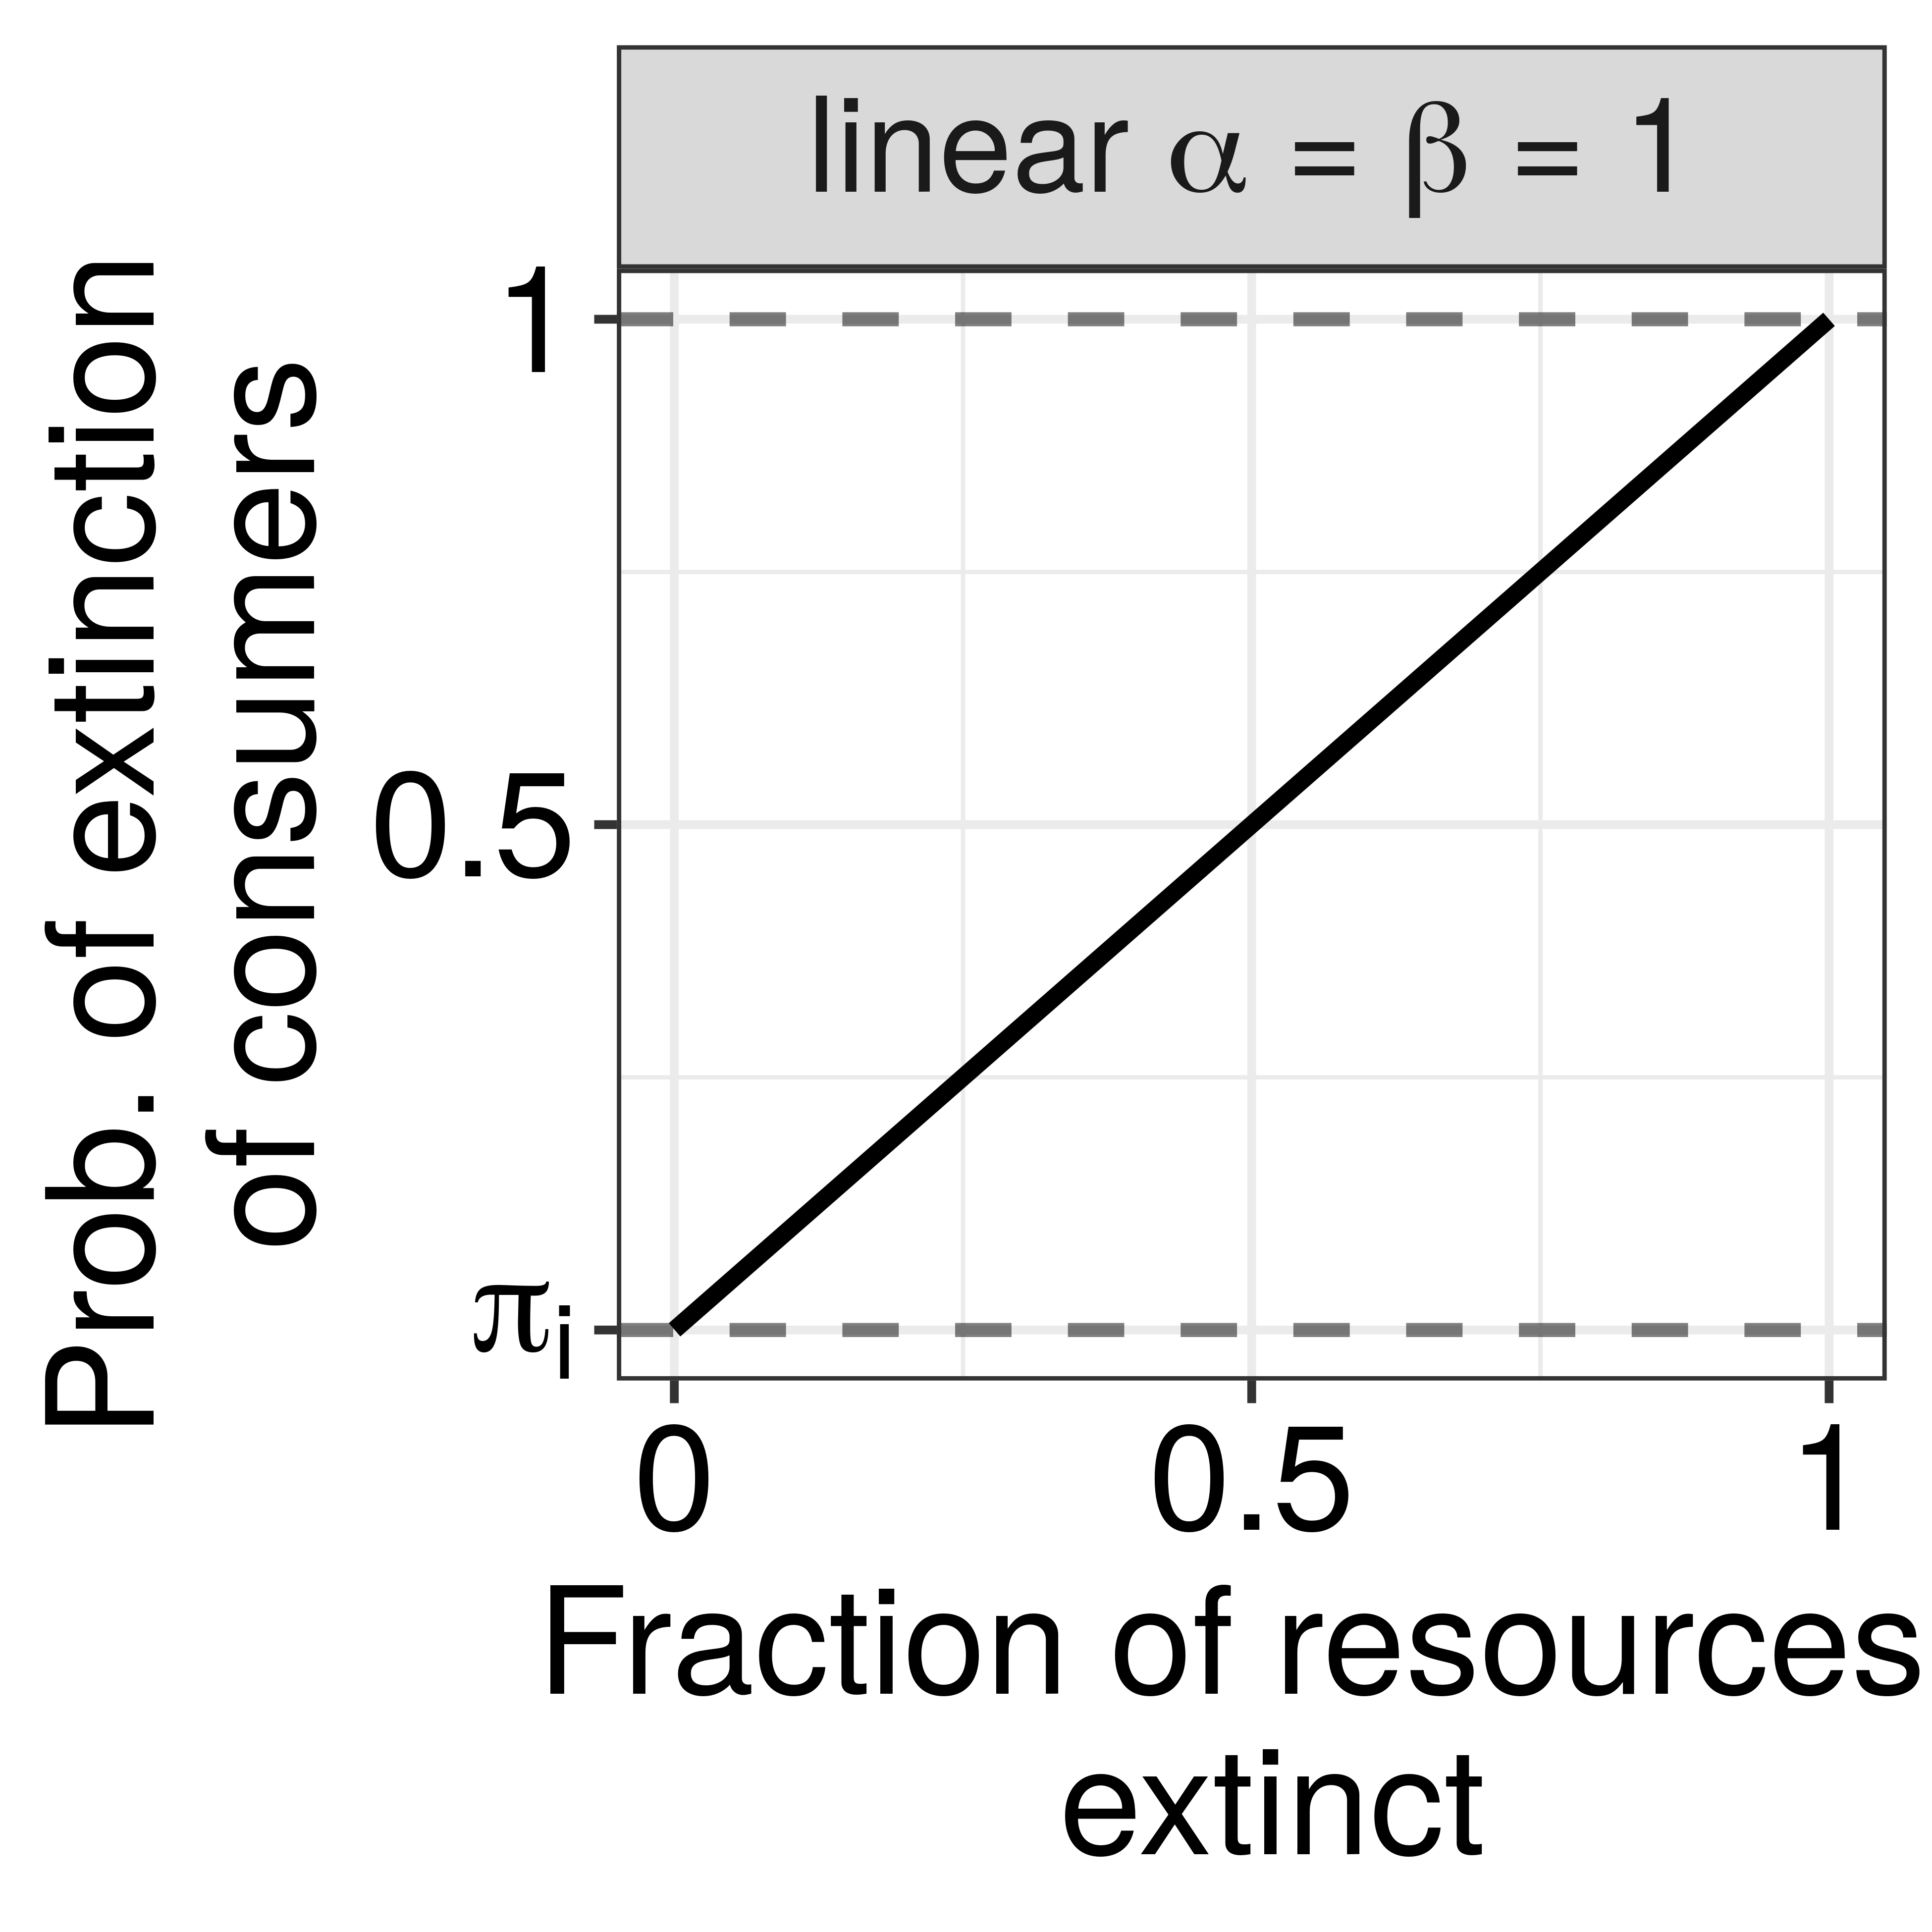
\includegraphics[width=0.19\textwidth,valign=t]{fform_1_1.png}
  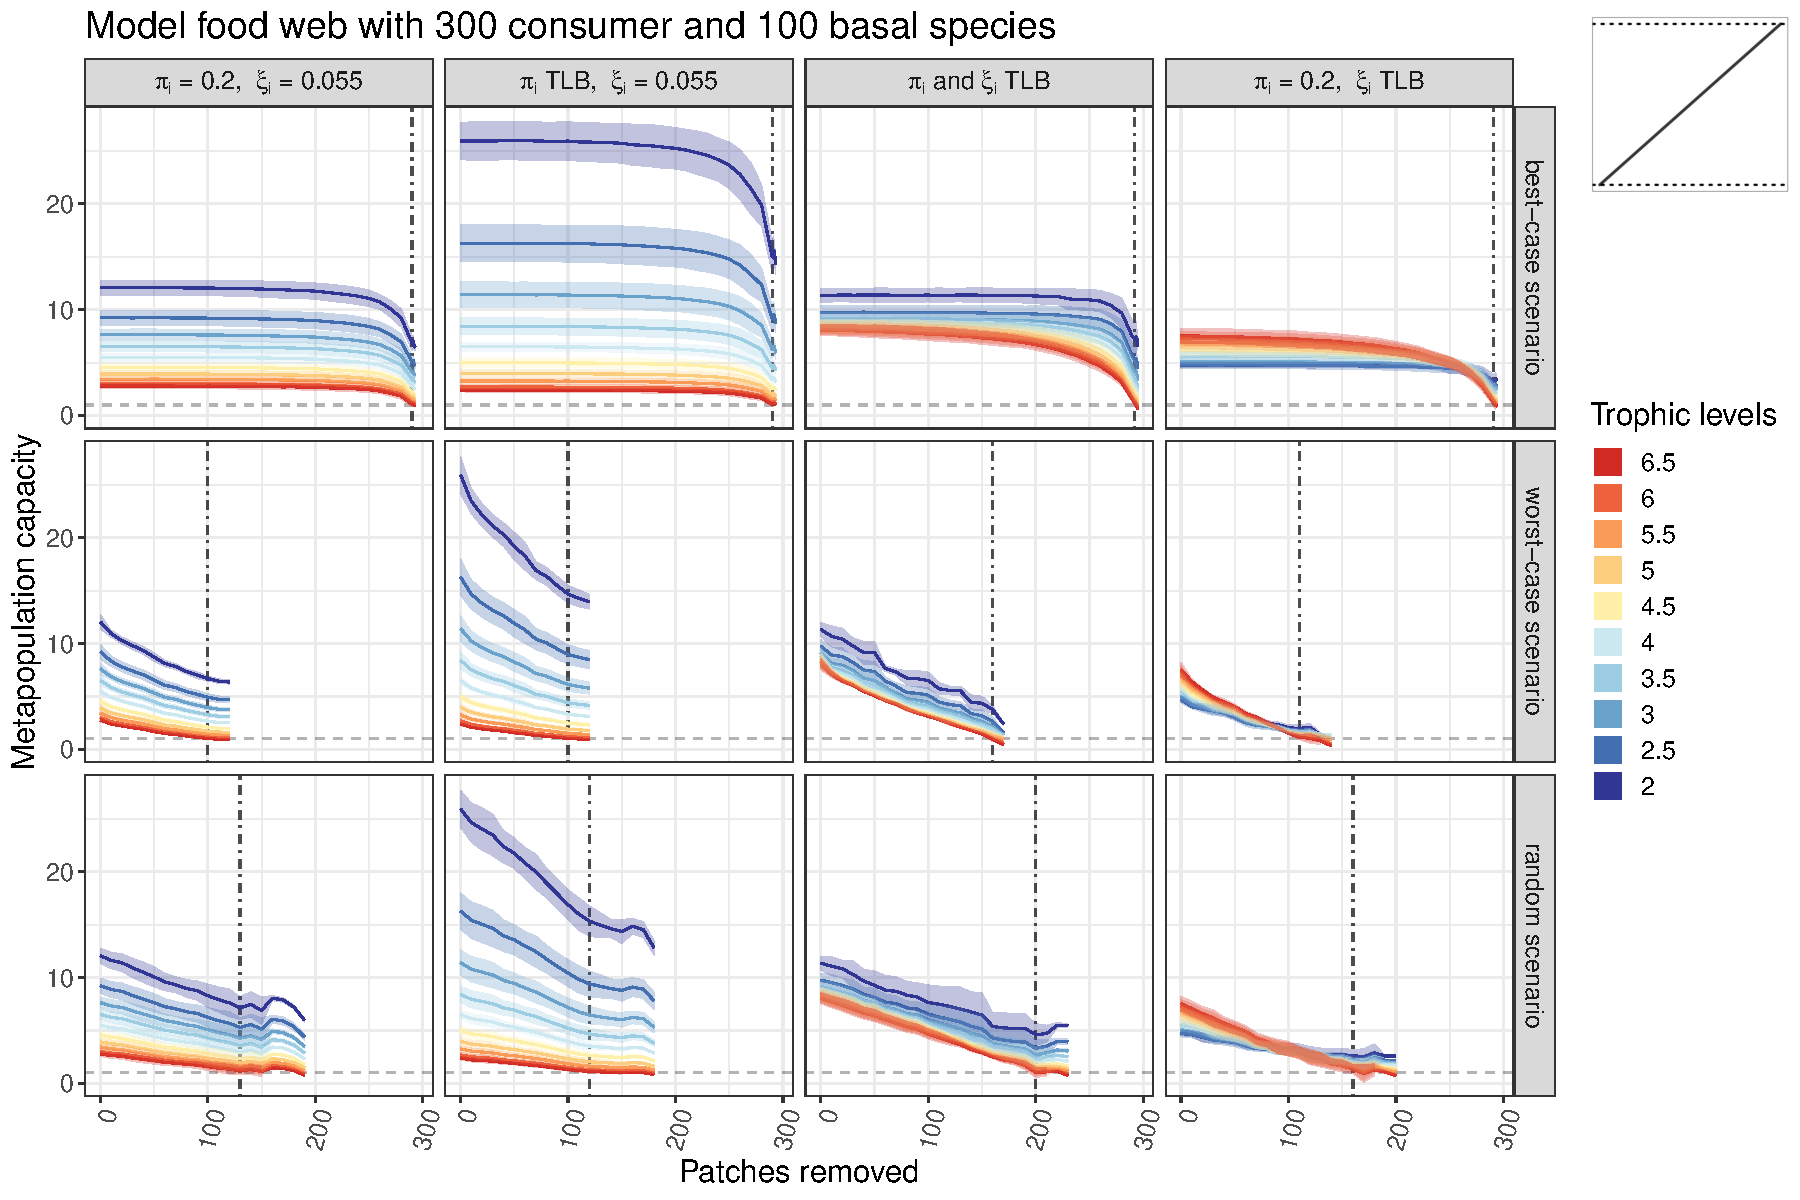
\includegraphics[width=0.8\textwidth,valign=t]{lambda_Model_food_web_with_300_consumer_and_100_basal_species_top_1_1.pdf}
  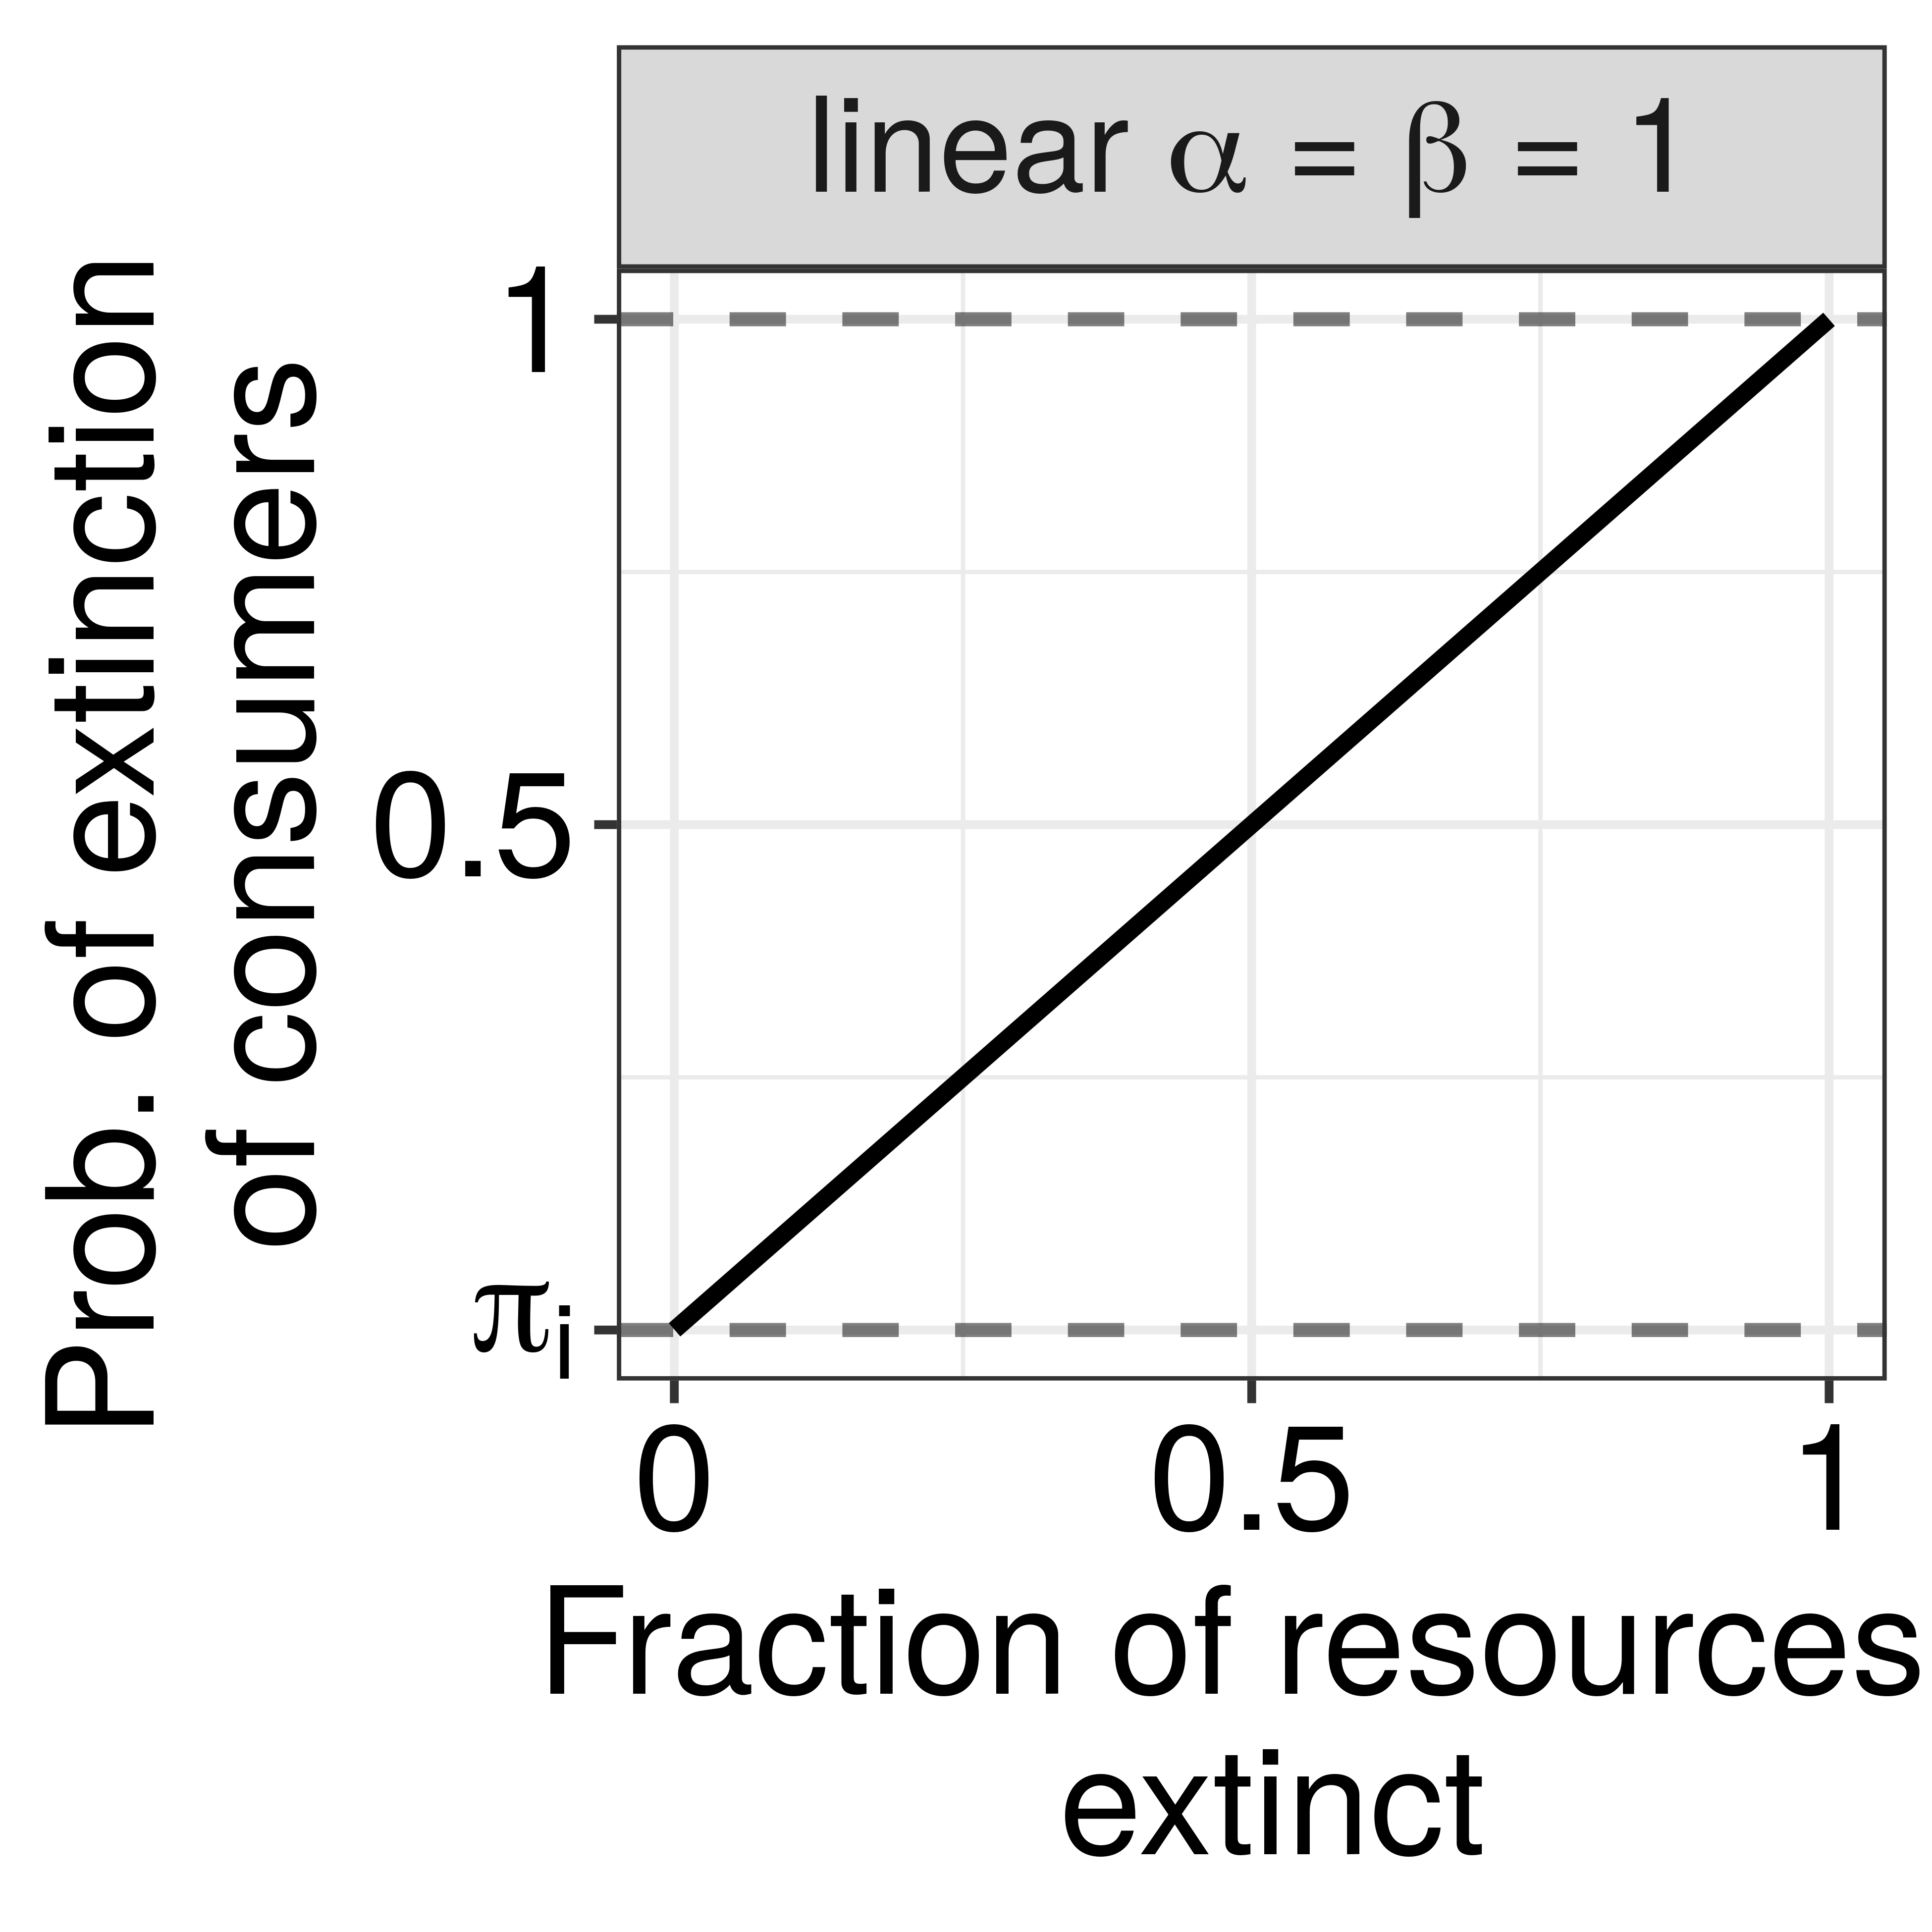
\includegraphics[width=0.19\textwidth,valign=t]{fform_1_1.png}
 \caption{As Figure~\ref{S_fig:patchloss_350_50_1}, but patch removal is based on the patch value rankings of top species, and only the linear consumer response to resource loss is implemented (top right insets). Here A-D are for model food webs with different numbers of consumer and basal species and E is for the Serengeti food web.}
 \label{S_fig:patchloss_top_1}
\end{figure}

\begin{figure}\ContinuedFloat 
 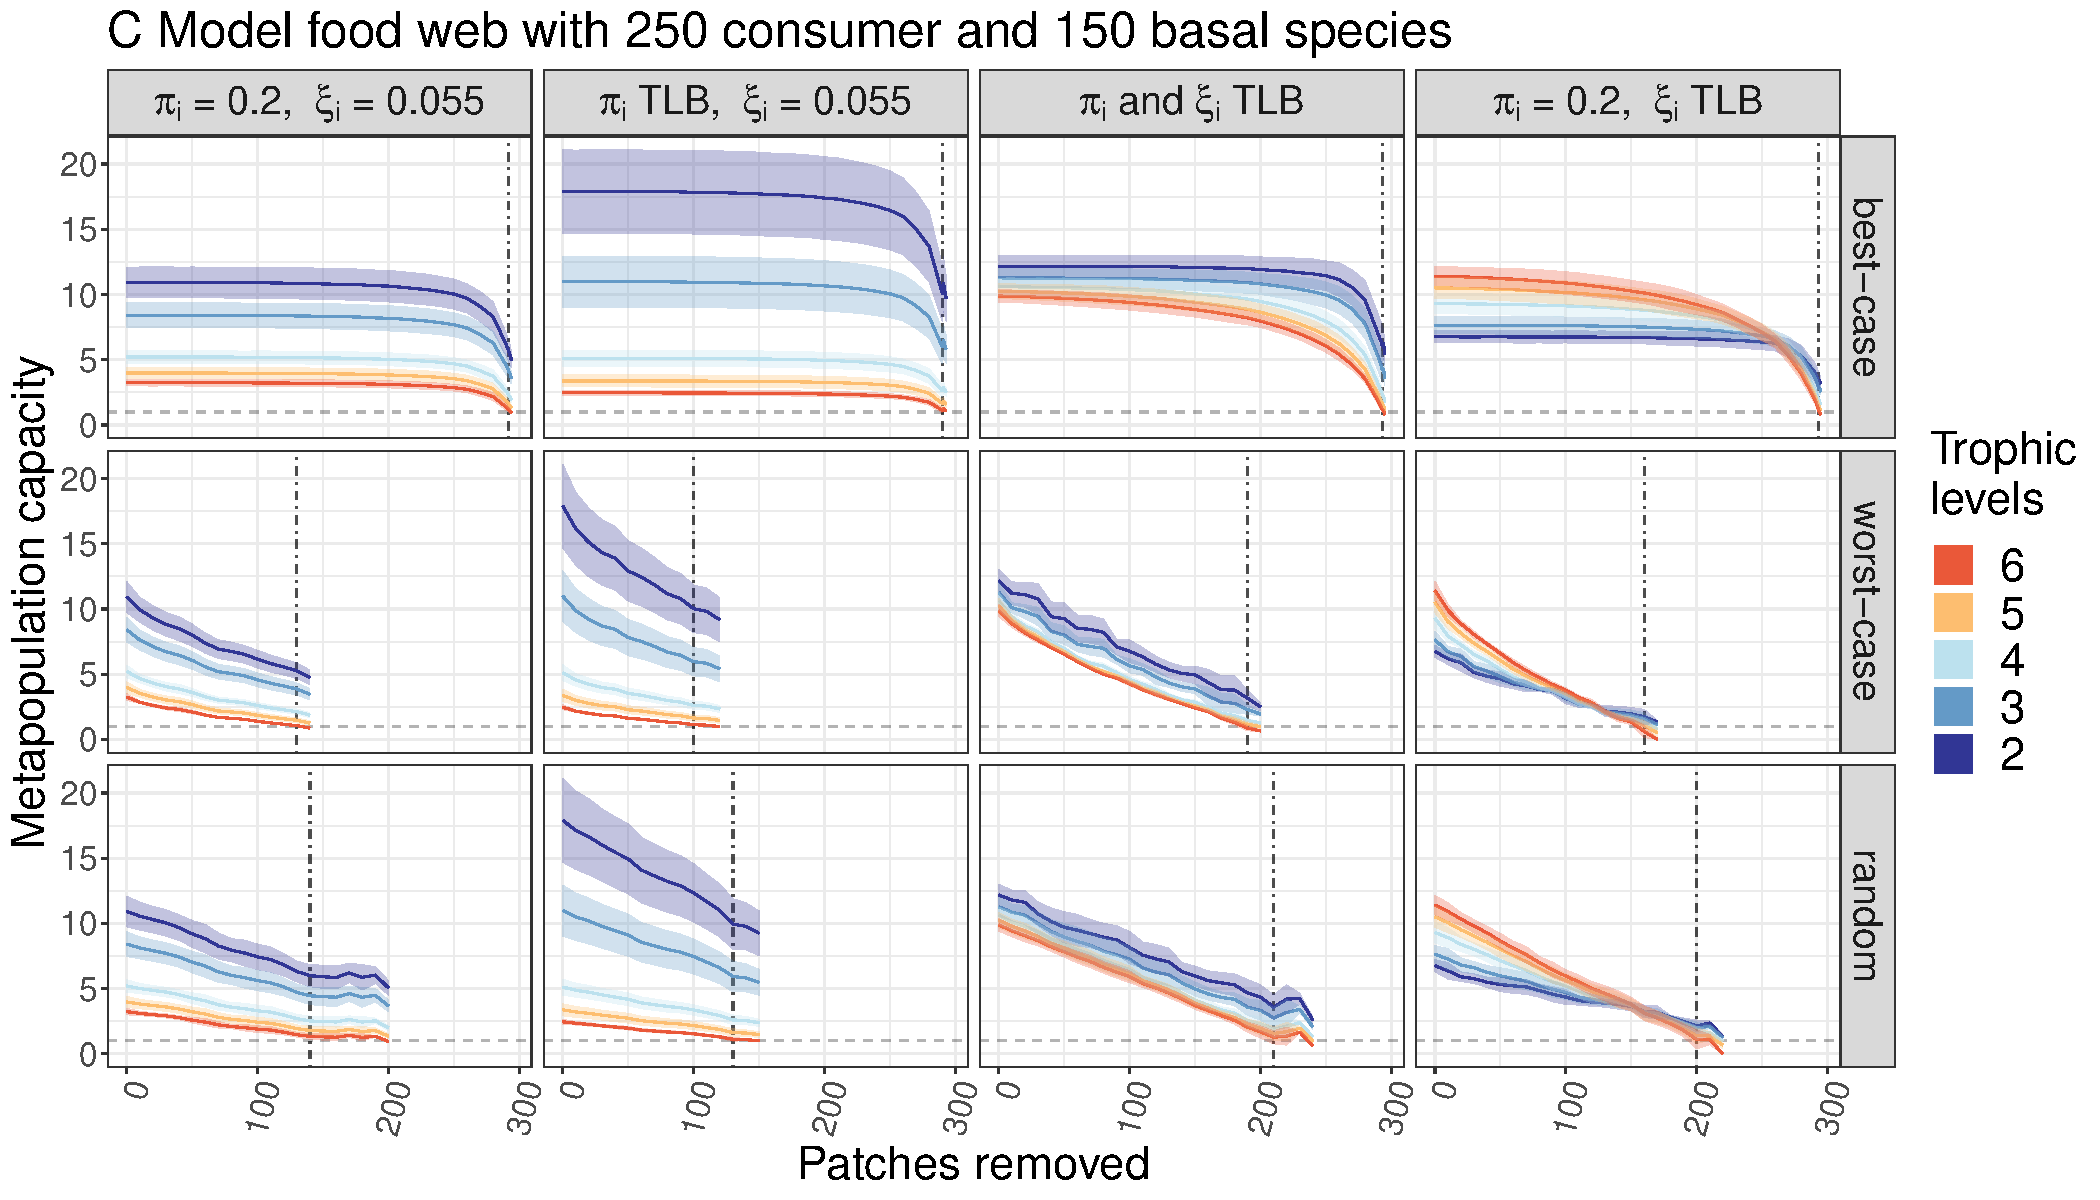
\includegraphics[width=0.8\textwidth,valign=t]{lambda_Model_food_web_with_250_consumer_and_150_basal_species_top_1_1.pdf}
  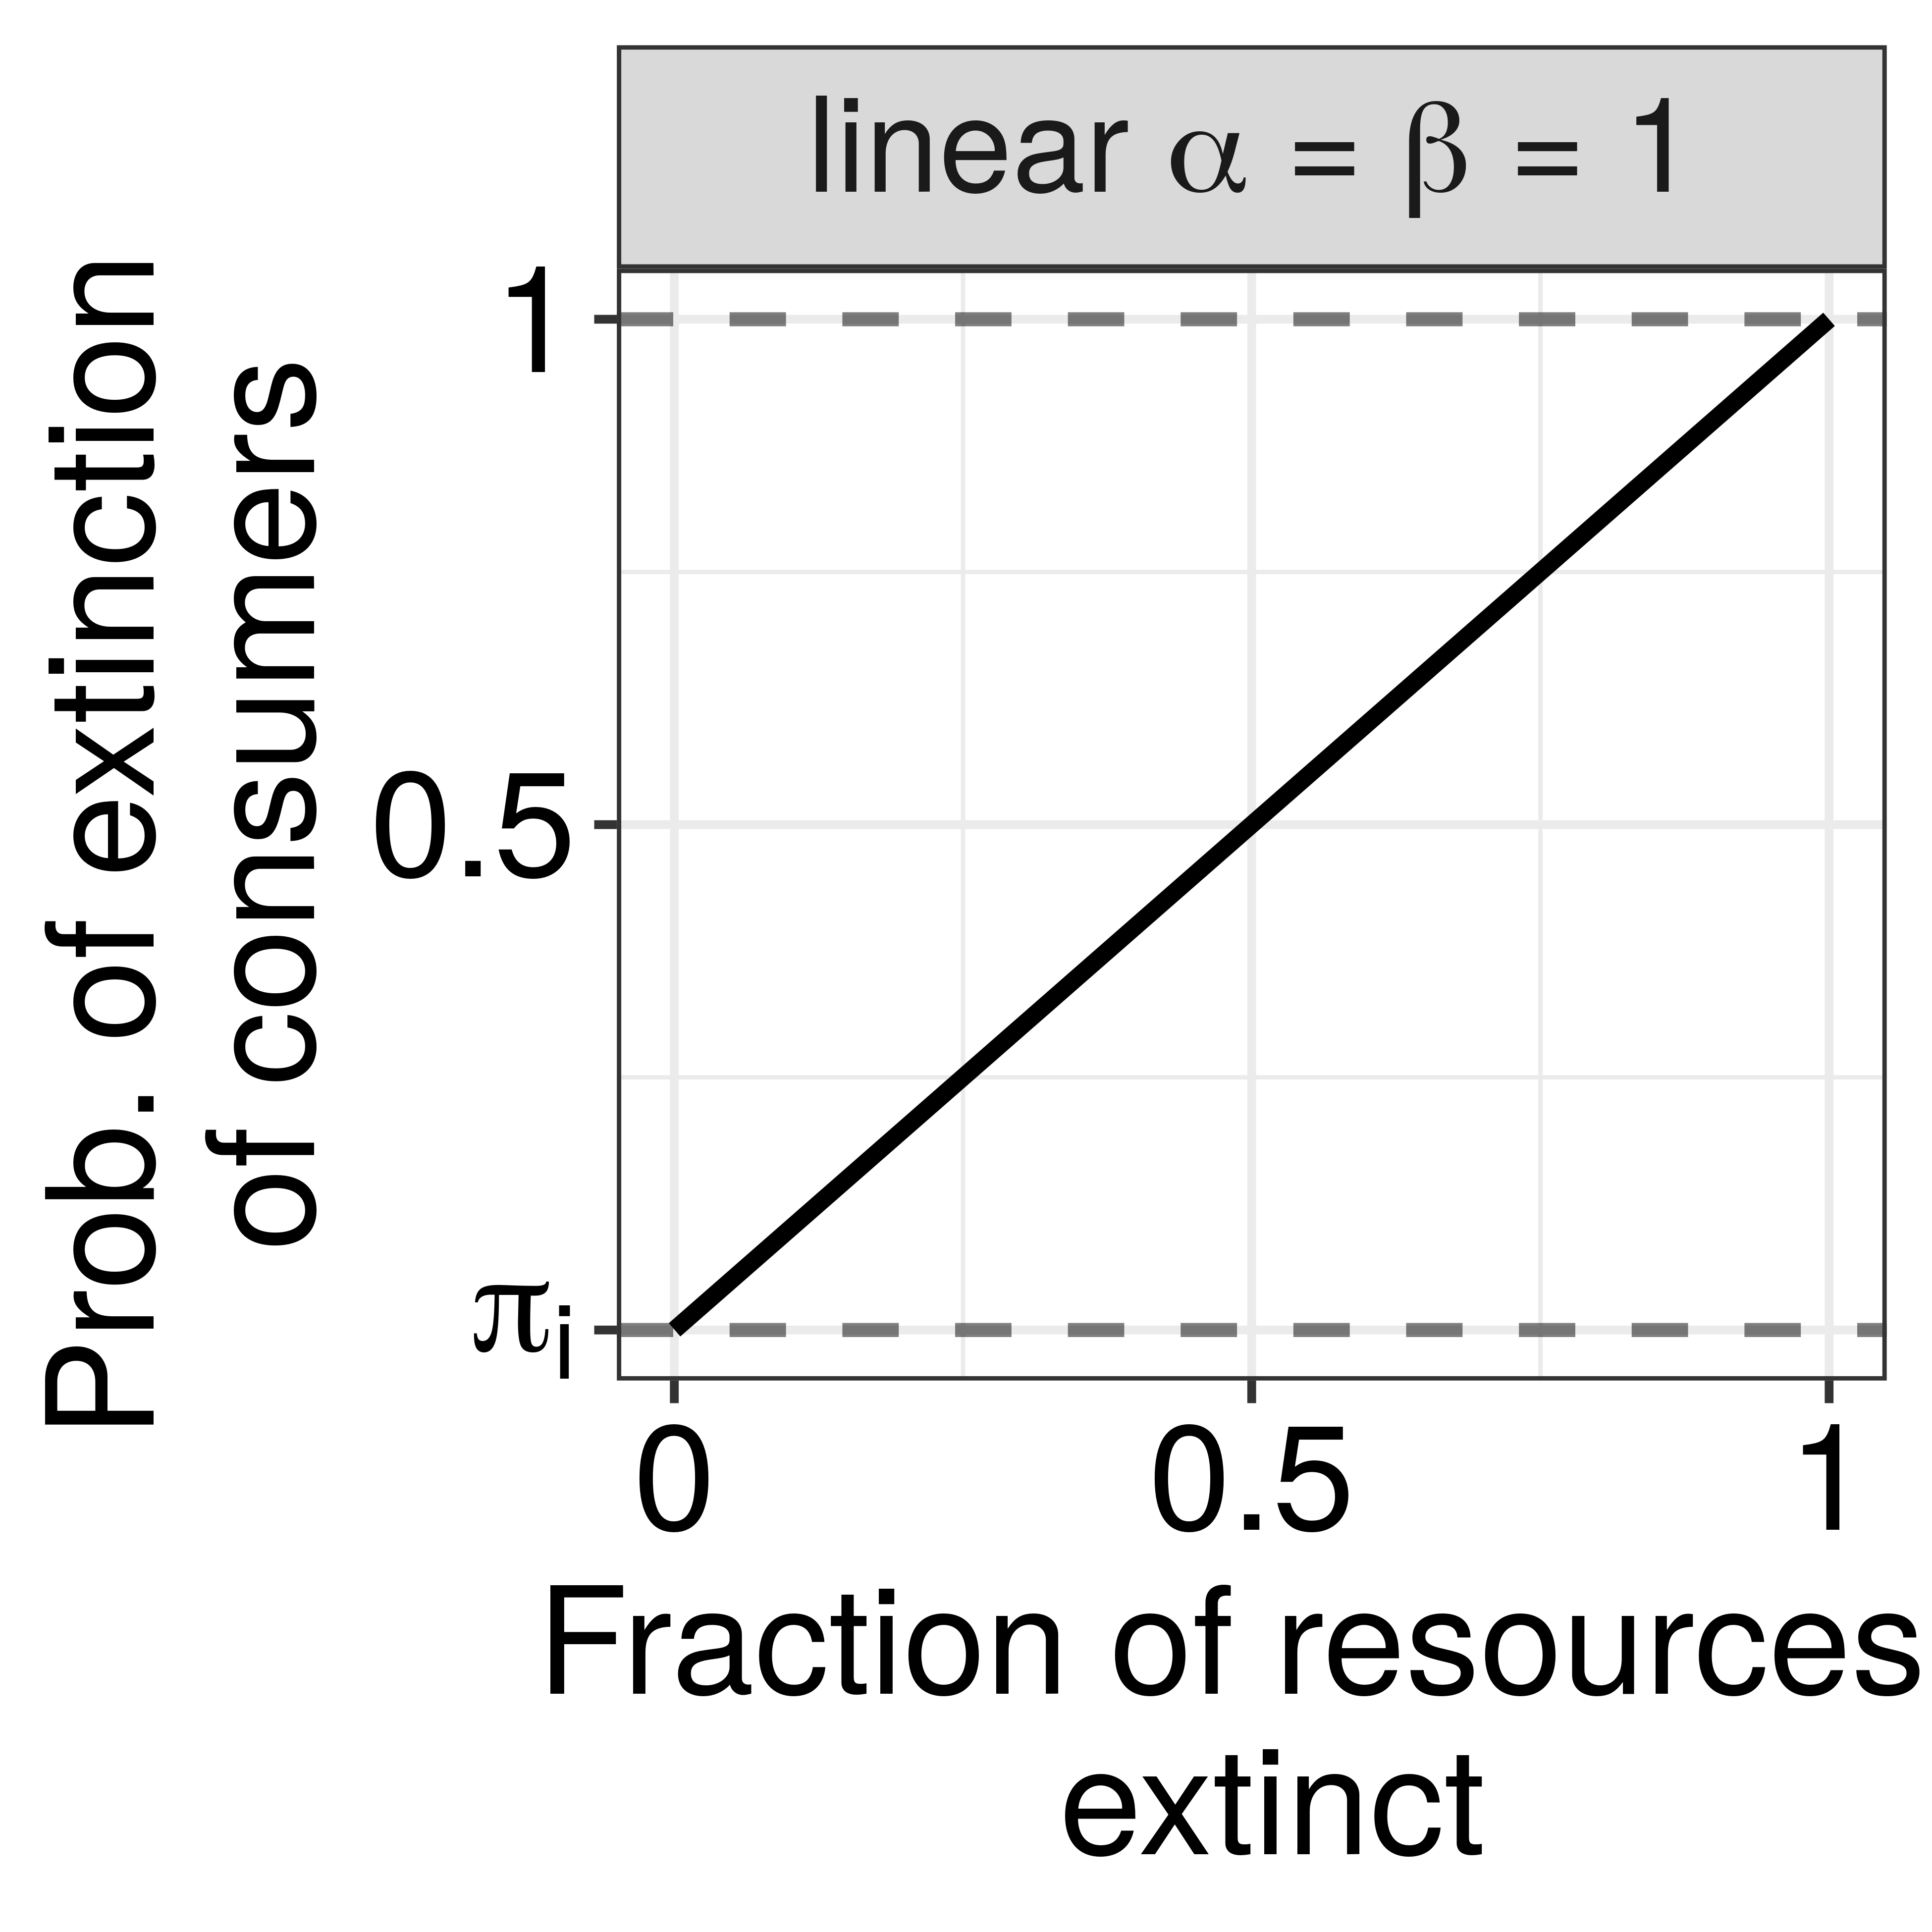
\includegraphics[width=0.19\textwidth,valign=t]{fform_1_1.png}
  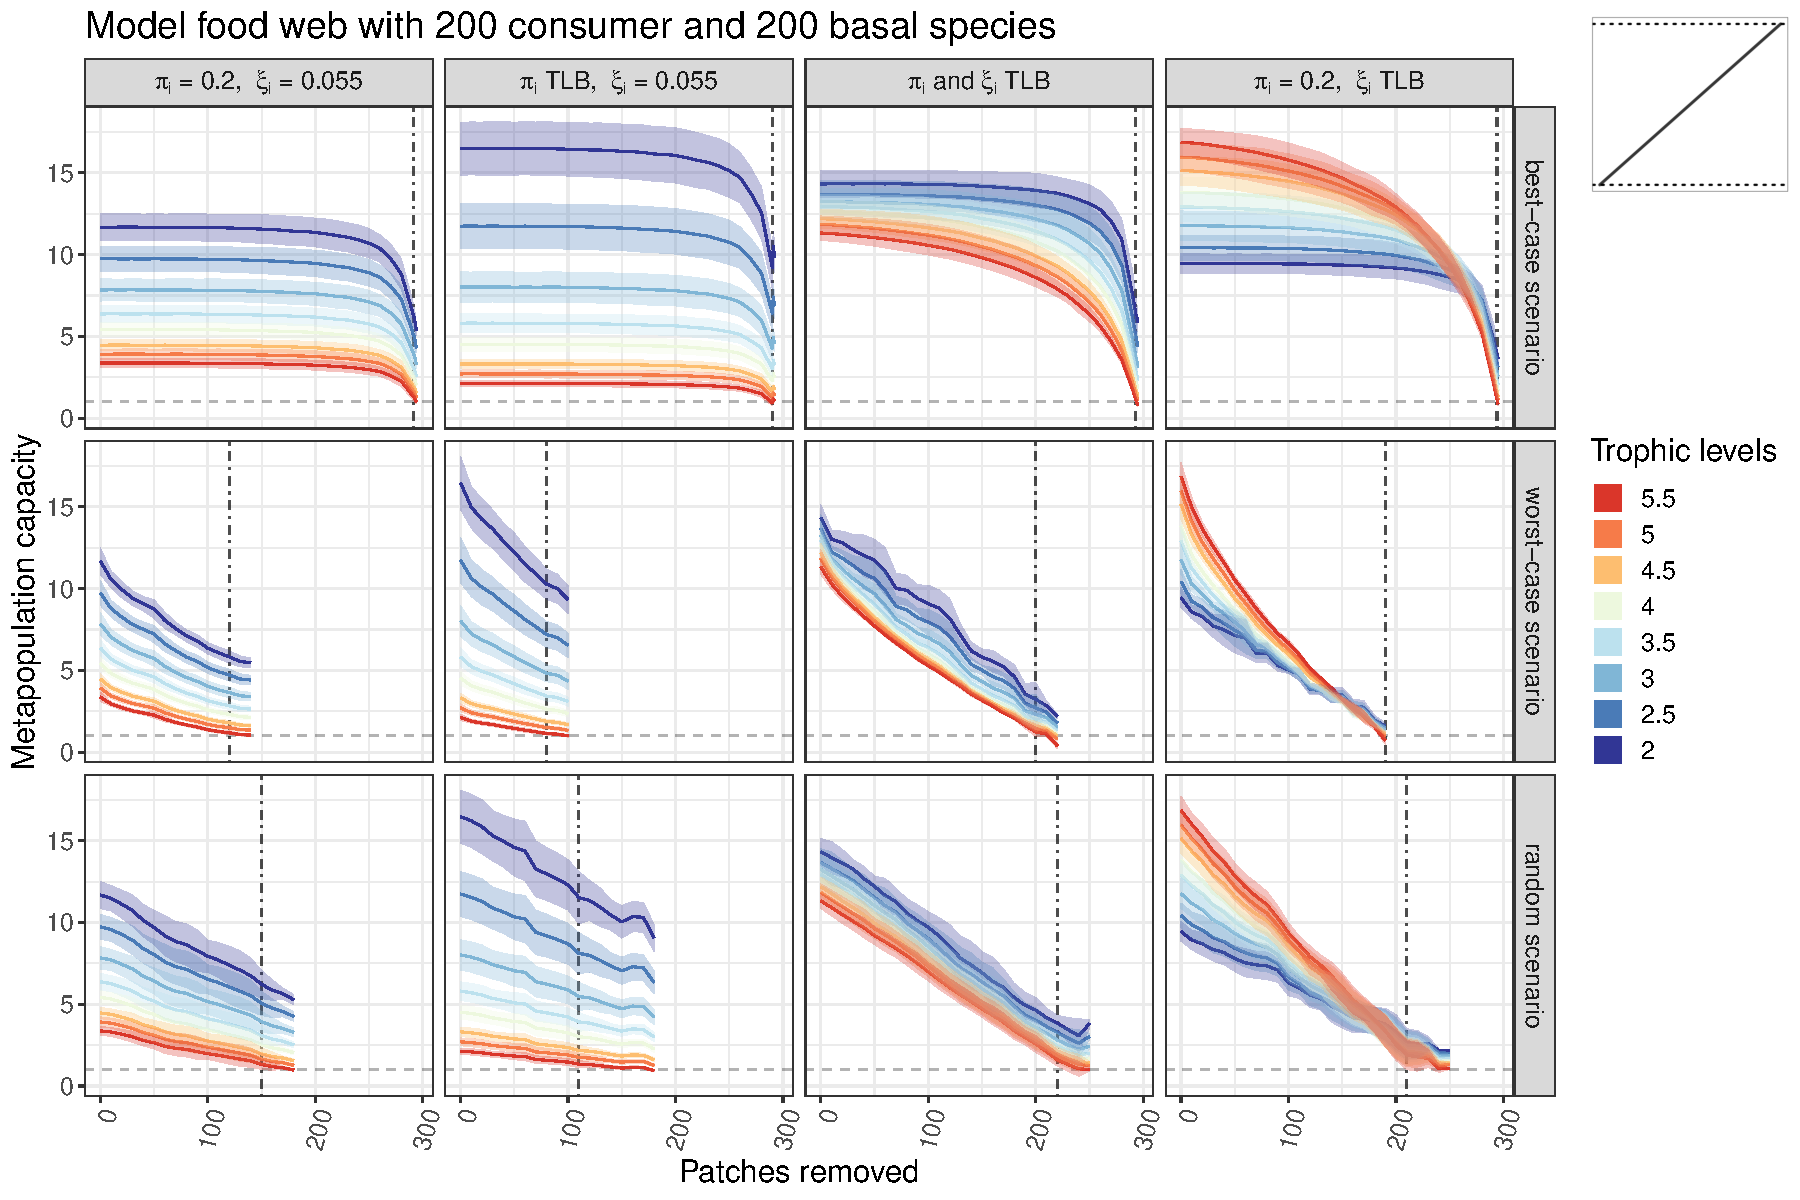
\includegraphics[width=0.8\textwidth,valign=t]{lambda_Model_food_web_with_200_consumer_and_200_basal_species_top_1_1.pdf}
  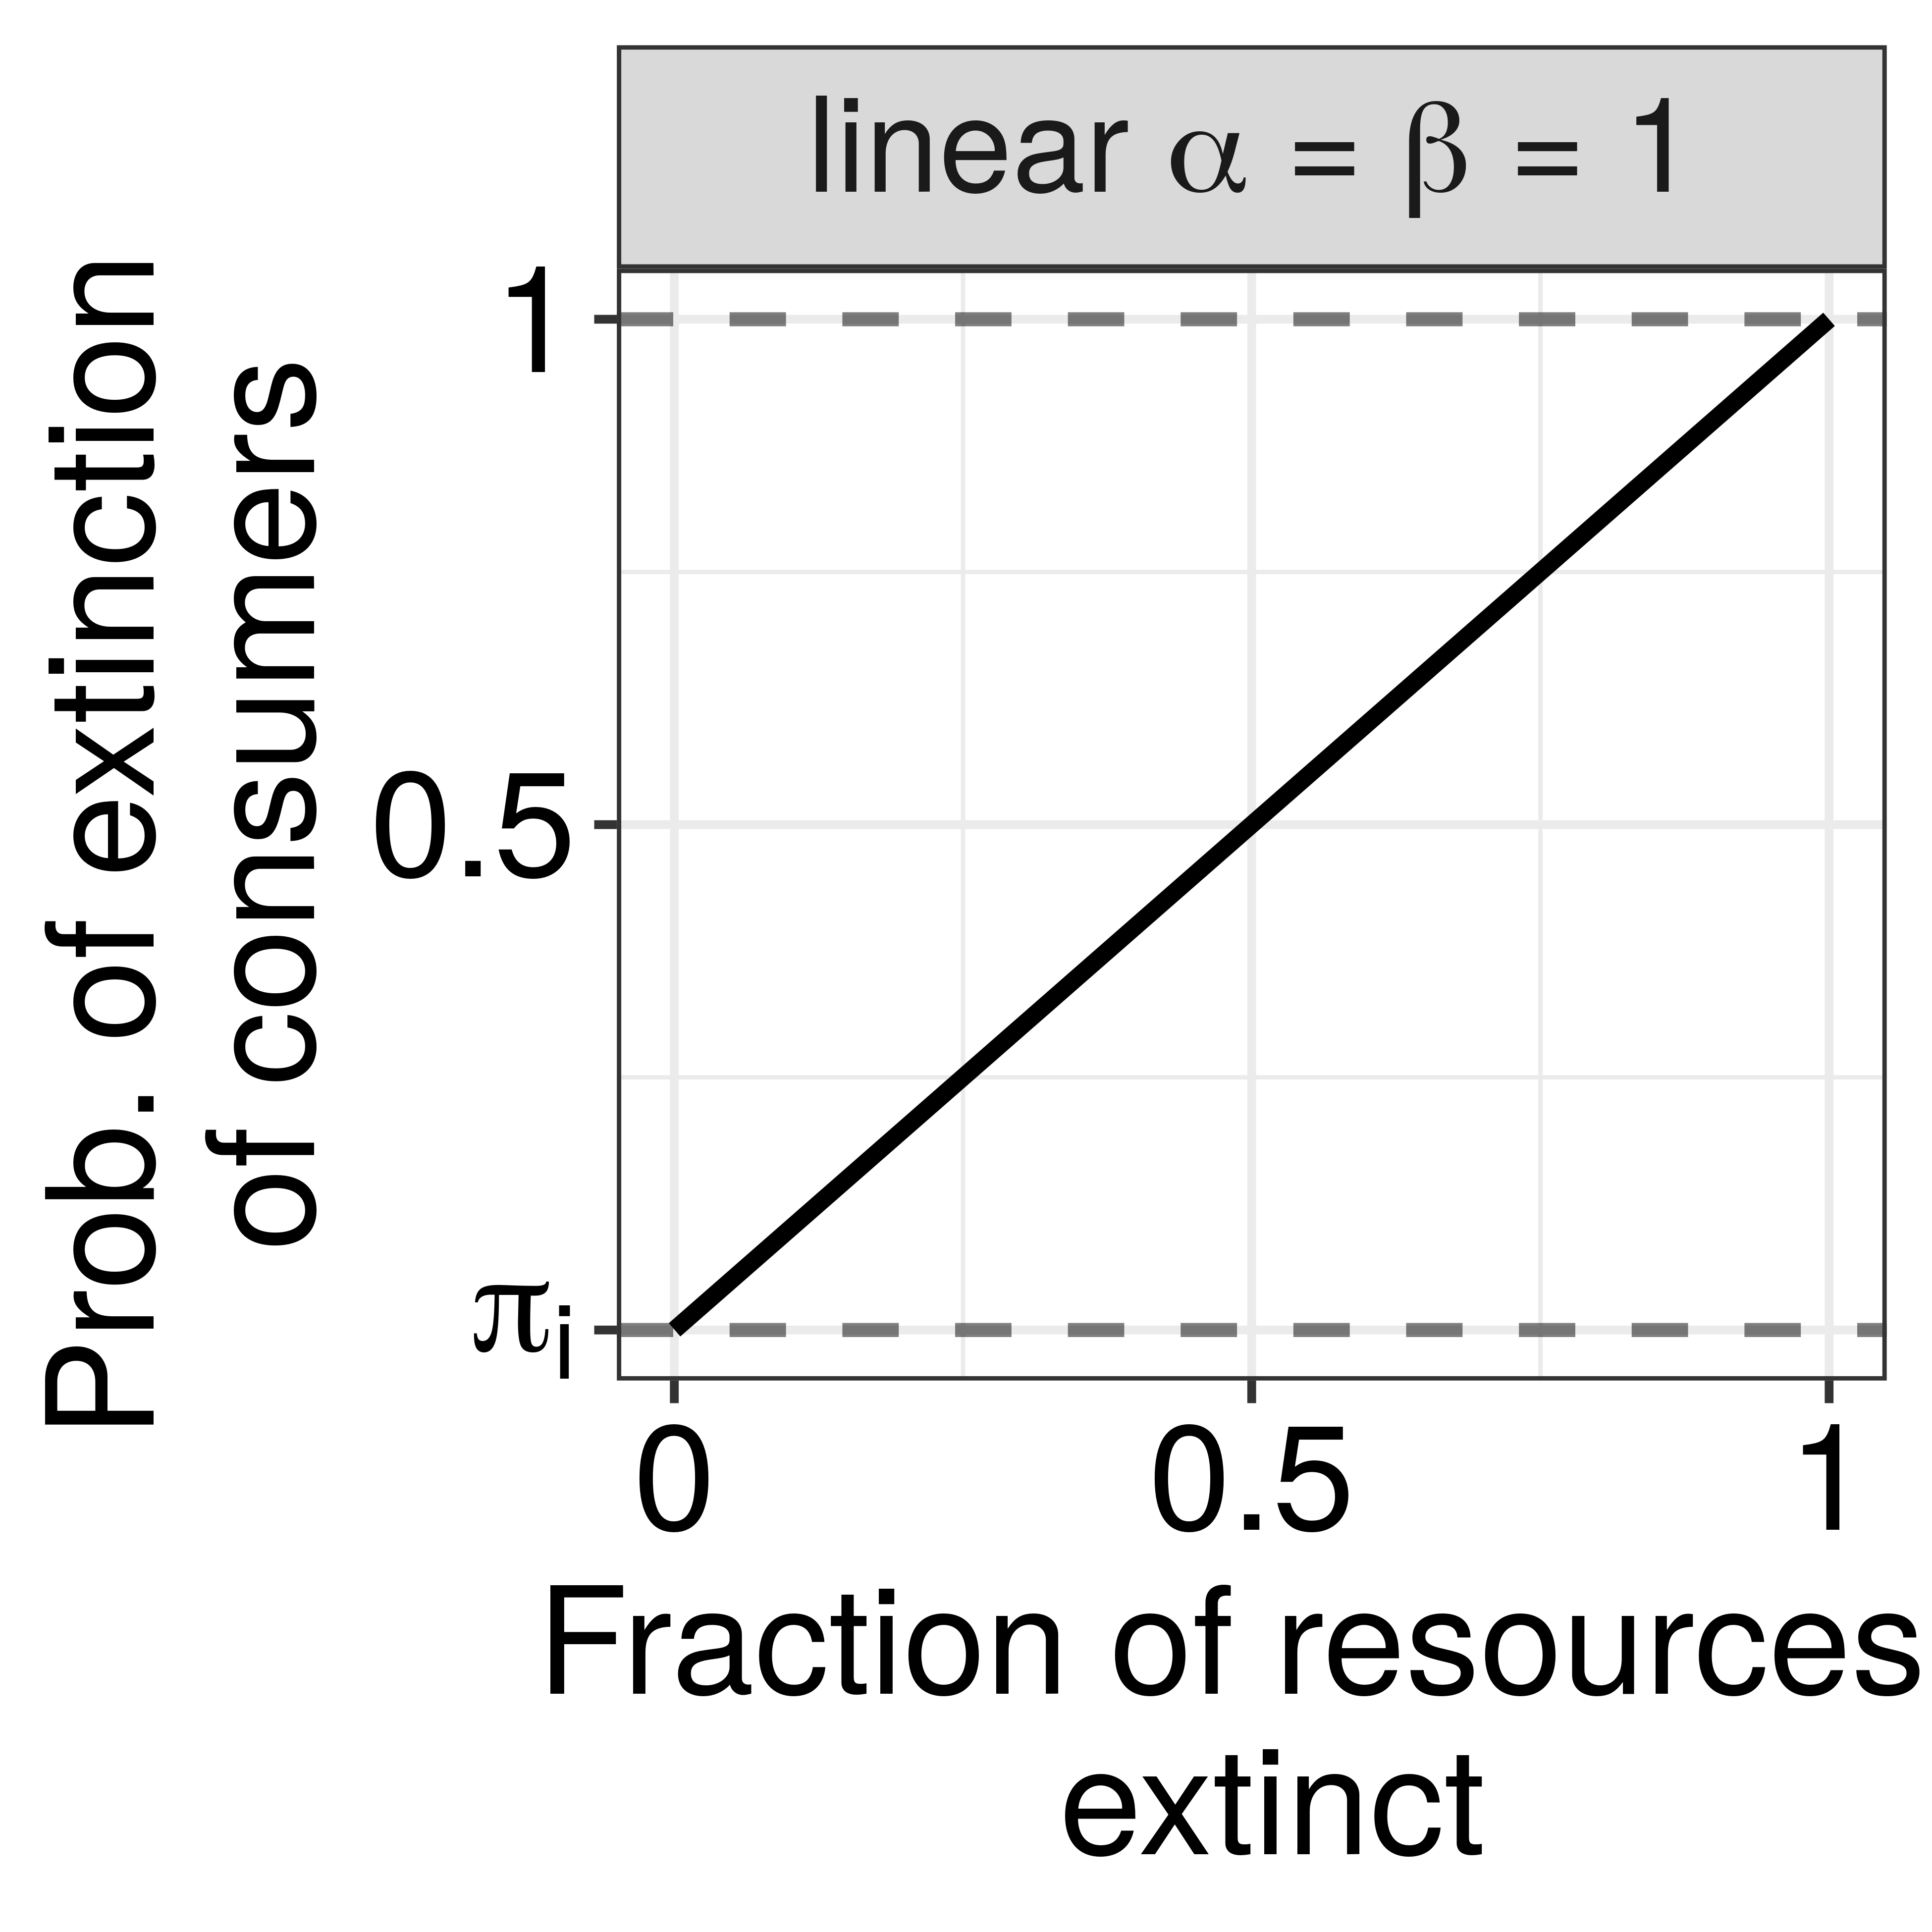
\includegraphics[width=0.19\textwidth,valign=t]{fform_1_1.png}
  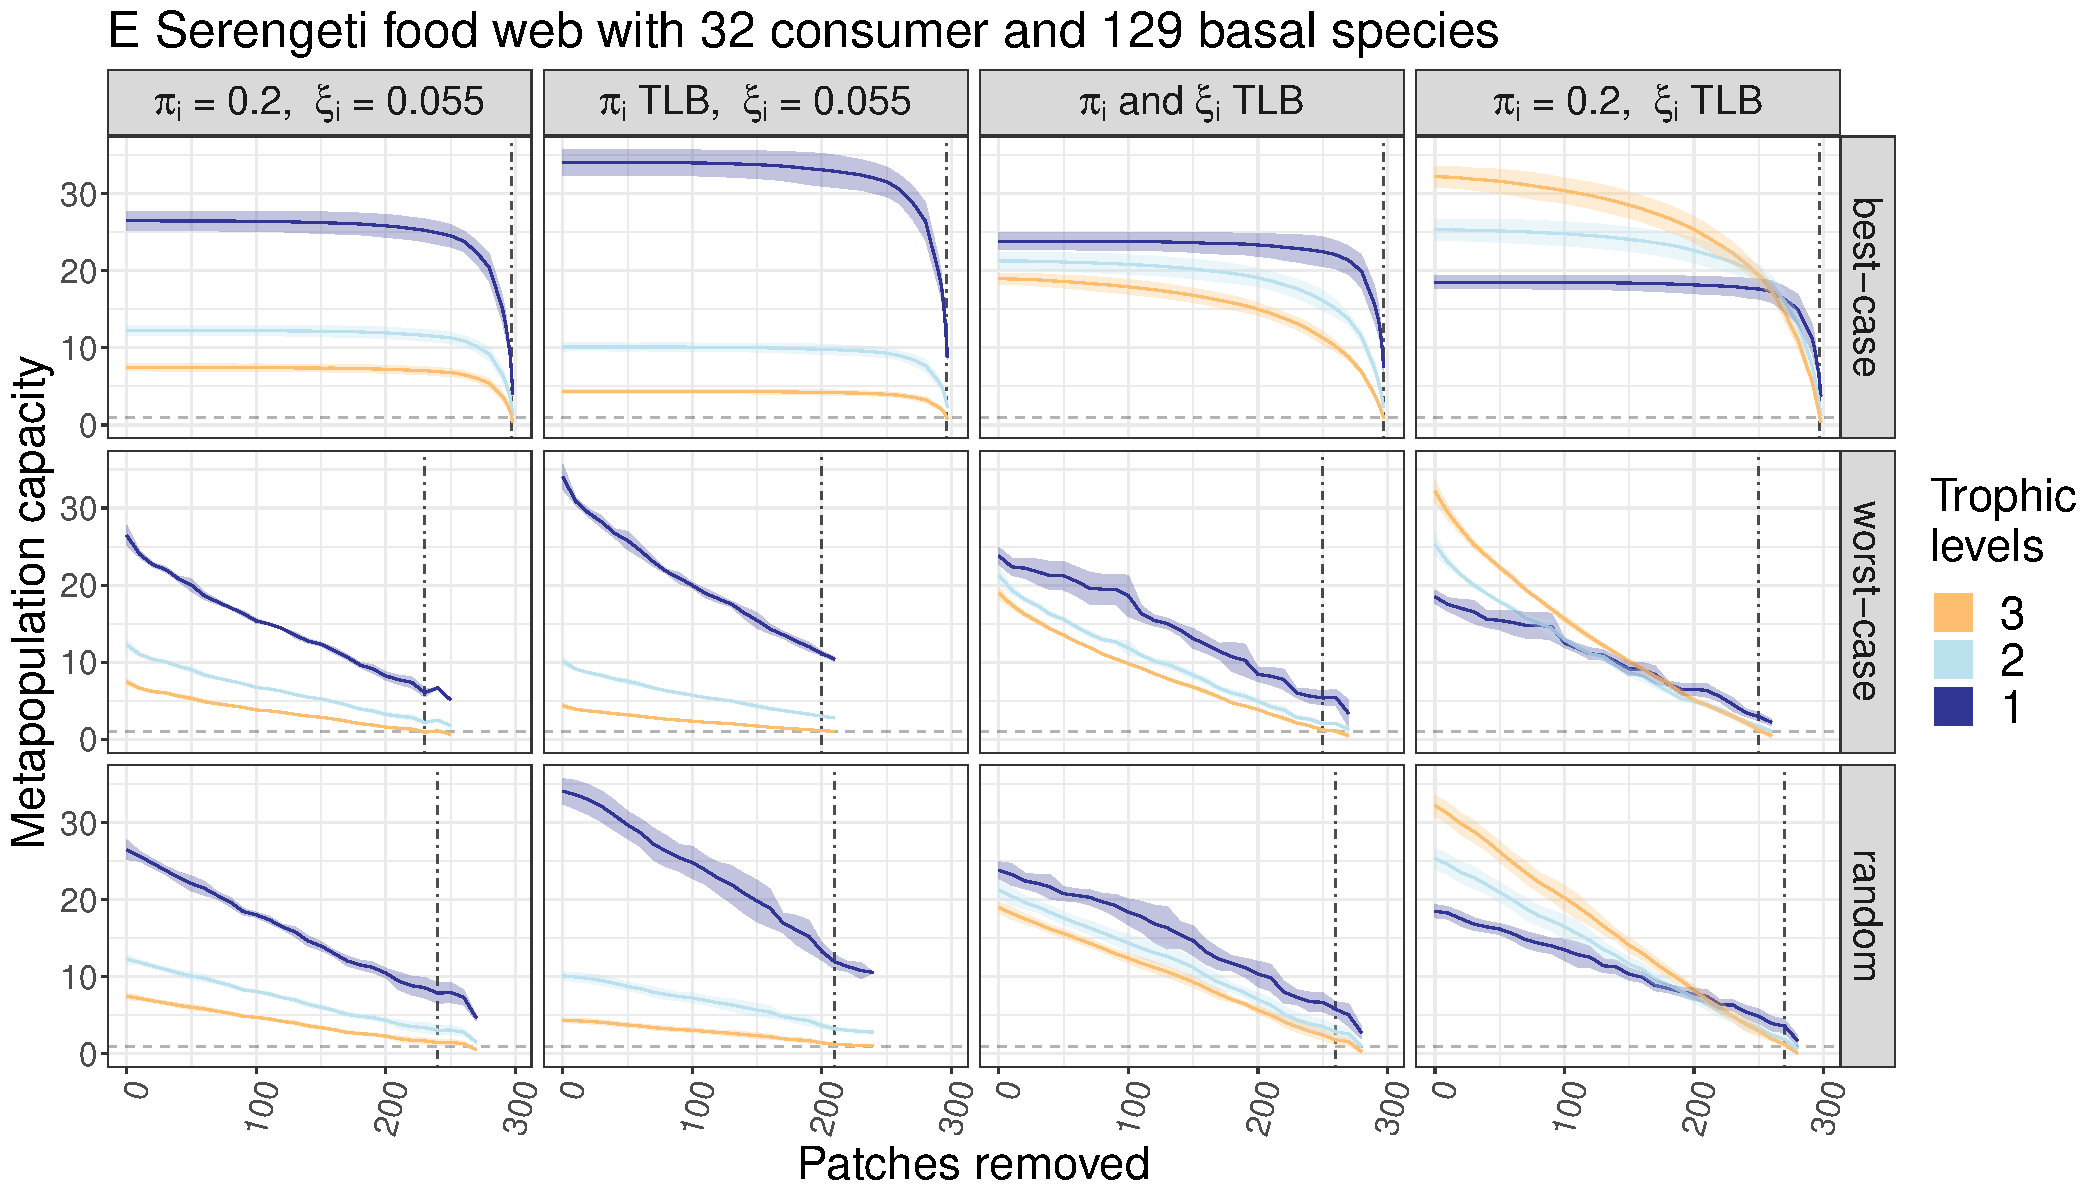
\includegraphics[width=0.8\textwidth,valign=t]{lambda_Serengeti_food_web_with_32_consumer_and_129_basal_species_top_1_1.pdf}
    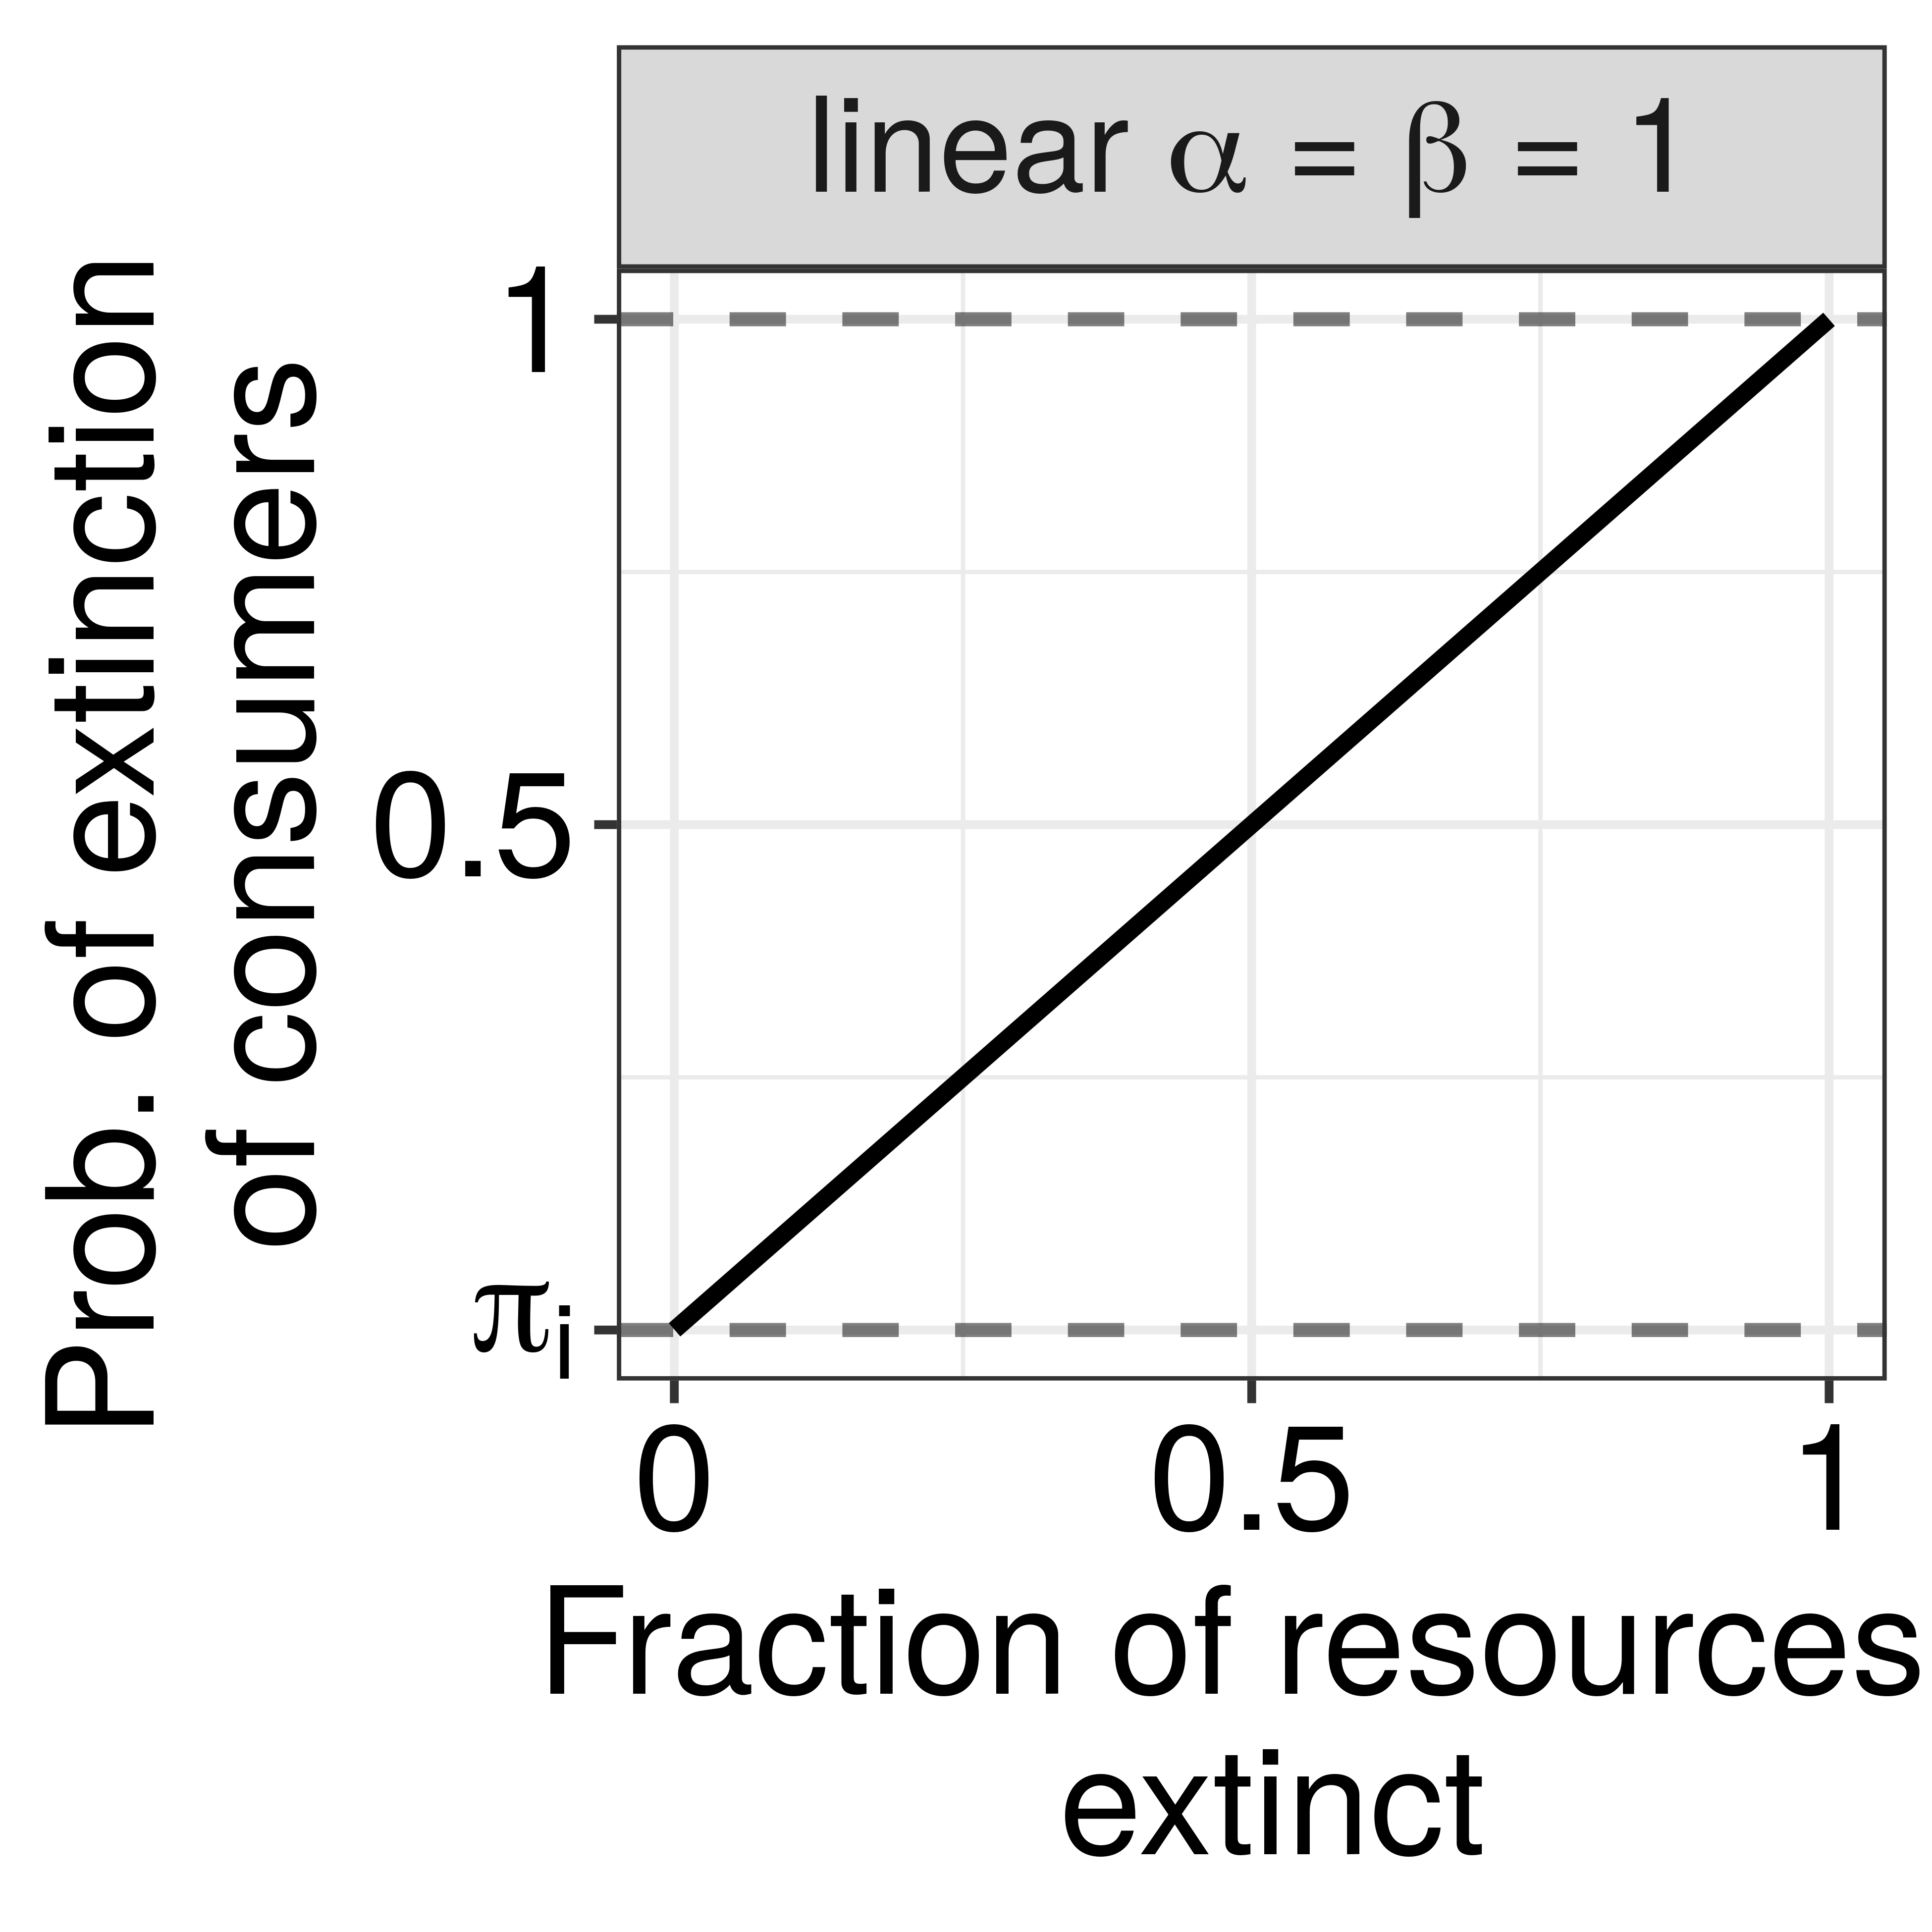
\includegraphics[width=0.19\textwidth,valign=t]{fform_1_1.png}
 \caption{Figure continued.}
 \label{S_fig:patchloss_top_2}
\end{figure}

\clearpage


\section{Assigning different weights to prey species in contributing to their predators' extinction risk} \label{sec:weighted}

So far, we have made the conditional extinction probability of consumers a function of the fraction of their prey items lost, regardless of the identity of those prey (Eq.~\ref{eq:BN_prob}). Here we relax this assumption by also accounting for the relative contribution of each prey to the predator's diet. Let $J_{ji}$ be the contribution of resource $i$ to the diet of consumer species $j$. We then define the weighted fraction $f'$ of $j$'s resources lost via
\begin{equation}
  \label{eq:fprime}
  f' = \frac{\sum_{\text{$j$ $\in$ absent}} J_{ji}}{
    \sum_{\text{$j$ $\in$ all prey}} J_{ji}} \ ,
\end{equation}
with the sum in the numerator going over prey that are absent, and the one in the denominator over all prey items of the consumer. So $f'$ is the fraction of resources lost weighted for their importance. With this definition, Eq.~\ref{eq:BN_prob} still holds, but we replace $f$ with $f'$:
\begin{equation}
  \label{eq:BN_prob_weighted}
  P(\neg C|f') = \pi_C + (1 - \pi_C) w(f') \ .
\end{equation}
We determine the $J_{ji}$ from a matrix of biomass flows at equilibrium. which we obtain as the Jacobian matrix evaluated at equilibrium (the community matrix) of the Allometric Trophic Network model (Section~\ref{sec:allo}, \citealp{Schneider2016}), which we have also used to generate our non-weighted trophic networks earlier.

Repeating the patch removal analysis for such a weighted version of our model food web with $50$ basal and $350$ consumer species, we get Figure~\ref{fig:patchloss_web1_11}. This is qualitatively identical to Figure~\ref{S_fig:patchloss_350_50_1}, which used the same setup but with non-weighted fractions of prey used (Eq.~\ref{eq:BN_prob}). This shows that the results are robust to relaxing the assumption that species contribute equally to consumers' diets.

\begin{figure}[!p] 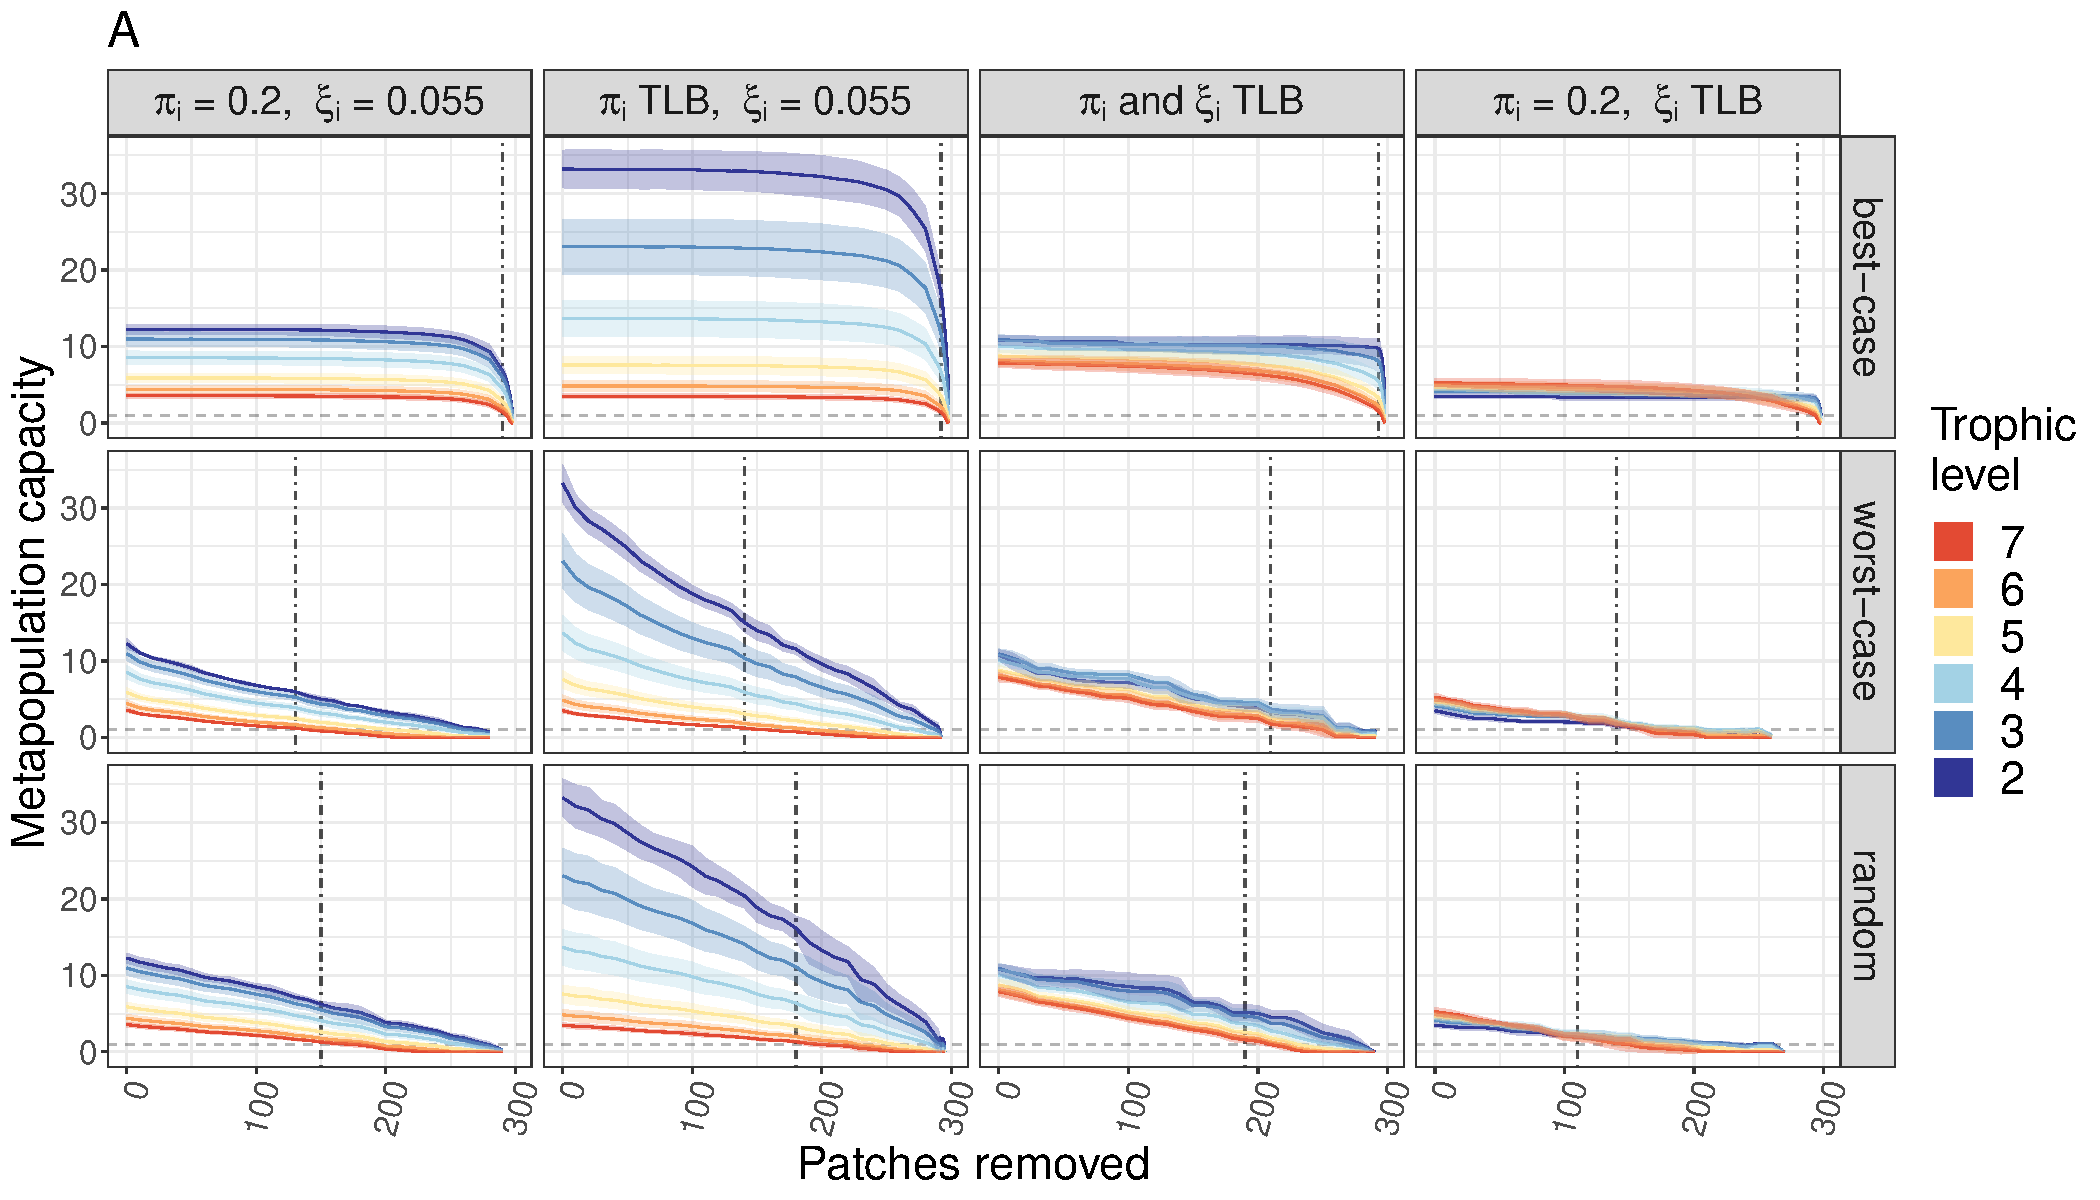
\includegraphics[width=0.8\textwidth,valign=t]{lambda_Weighted_Model_food_web_with_350_consumer_and_50_basal_species_(1)_basal_1_1.pdf}
  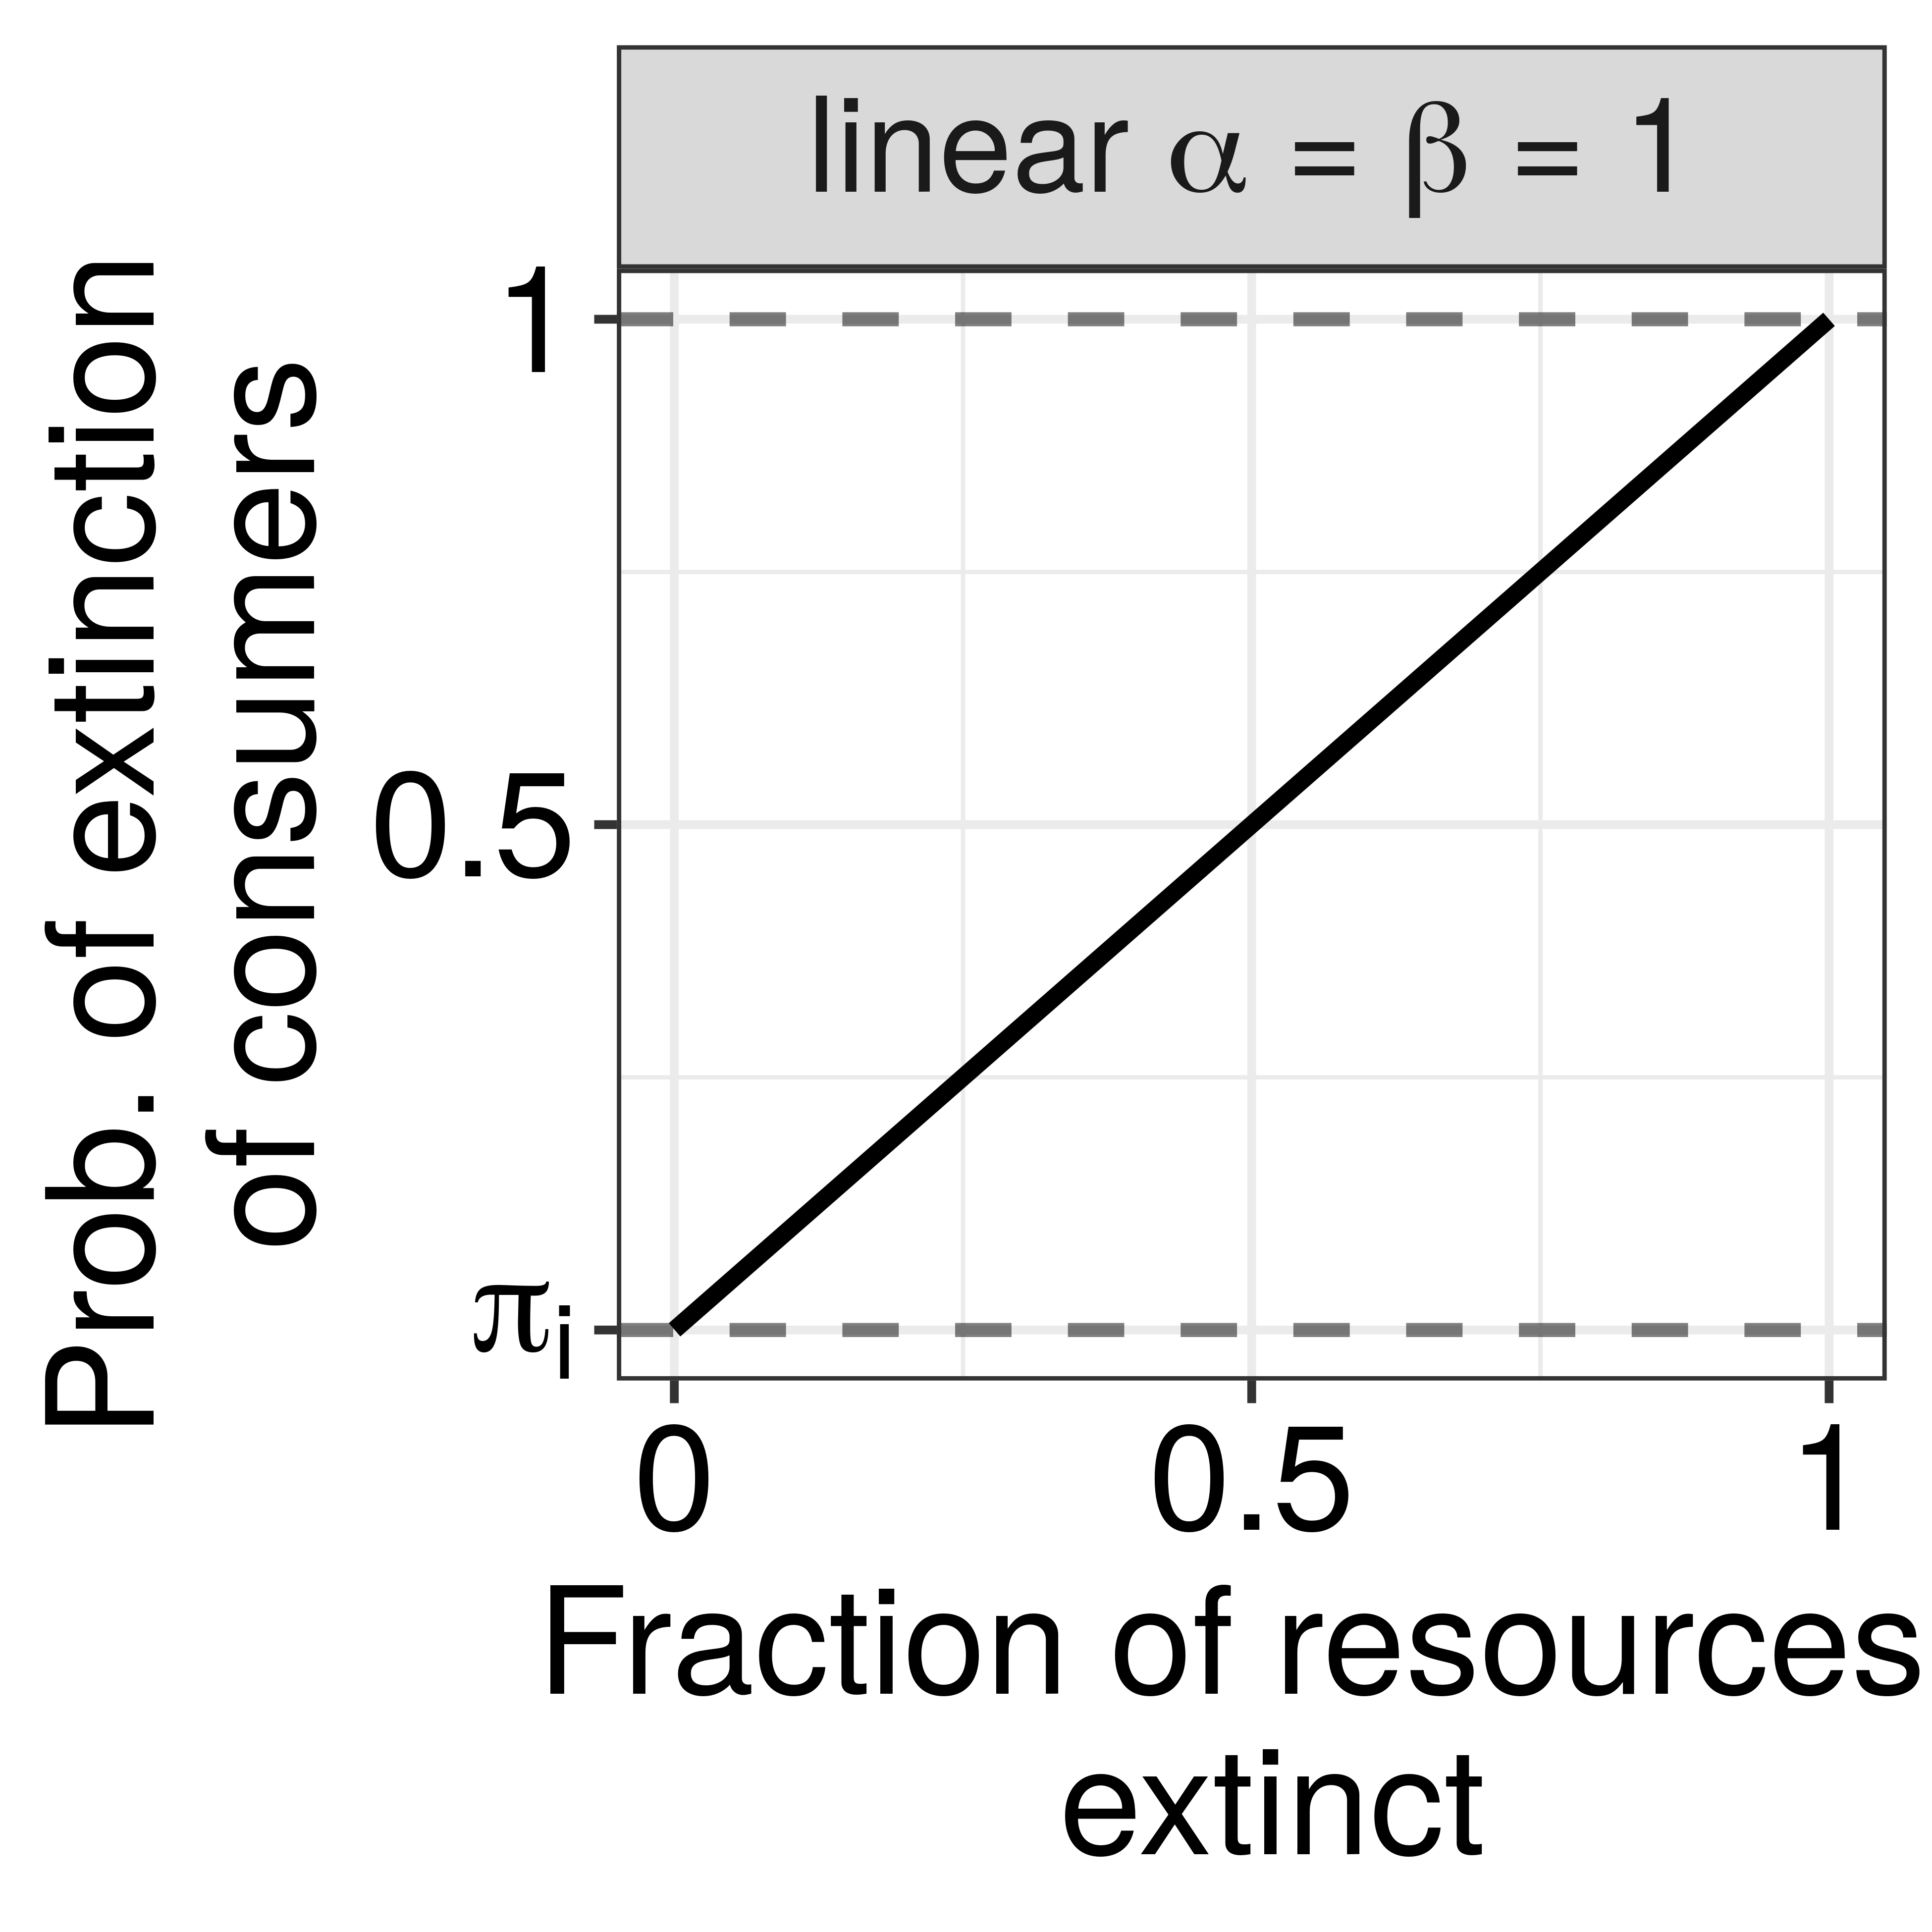
\includegraphics[width=0.19\textwidth,valign=t]{fform_1_1.png}
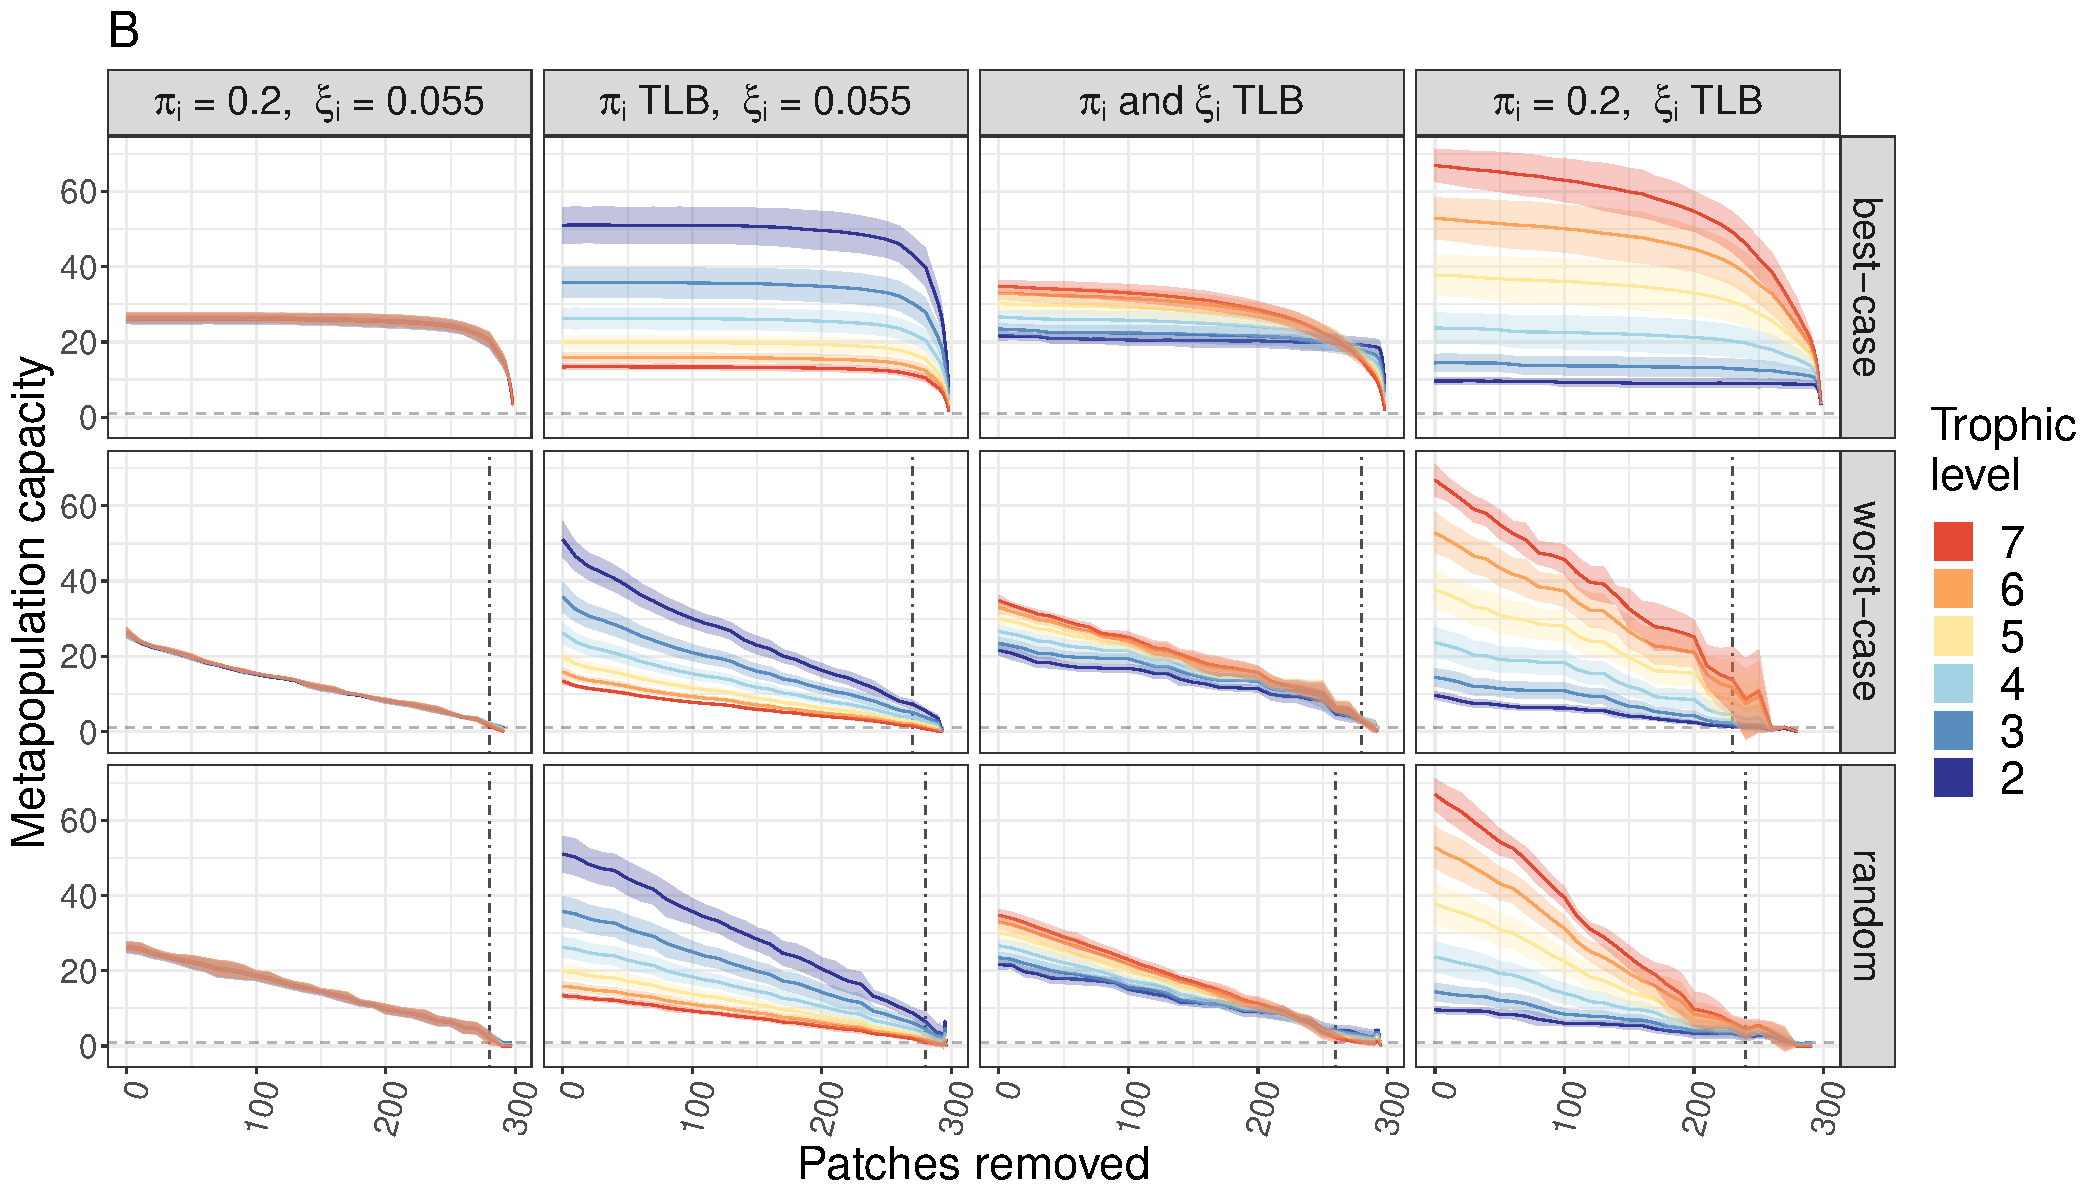
\includegraphics[width=0.8\textwidth,valign=t]{lambda_Weighted_Model_food_web_with_350_consumer_and_50_basal_species_(1)_basal_5_1.pdf}
  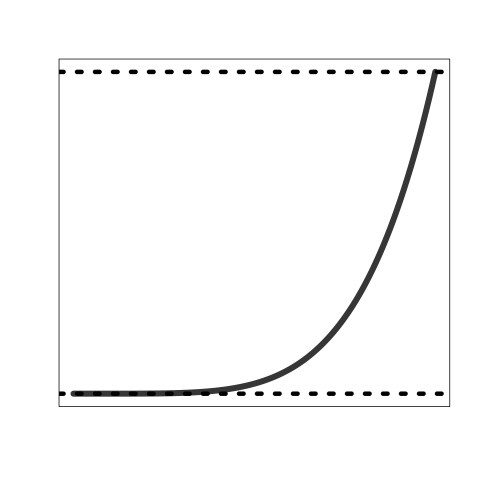
\includegraphics[width=0.19\textwidth,valign=t]{fform_5_1.png}
  \caption{As Figure~\ref{S_fig:patchloss_350_50_1}, but with a weighted food web. Results are qualitatively unchanged compared with the non-weighted case.}
  \label{fig:patchloss_web1_11}
\end{figure}

\begin{figure}[!p]\ContinuedFloat 
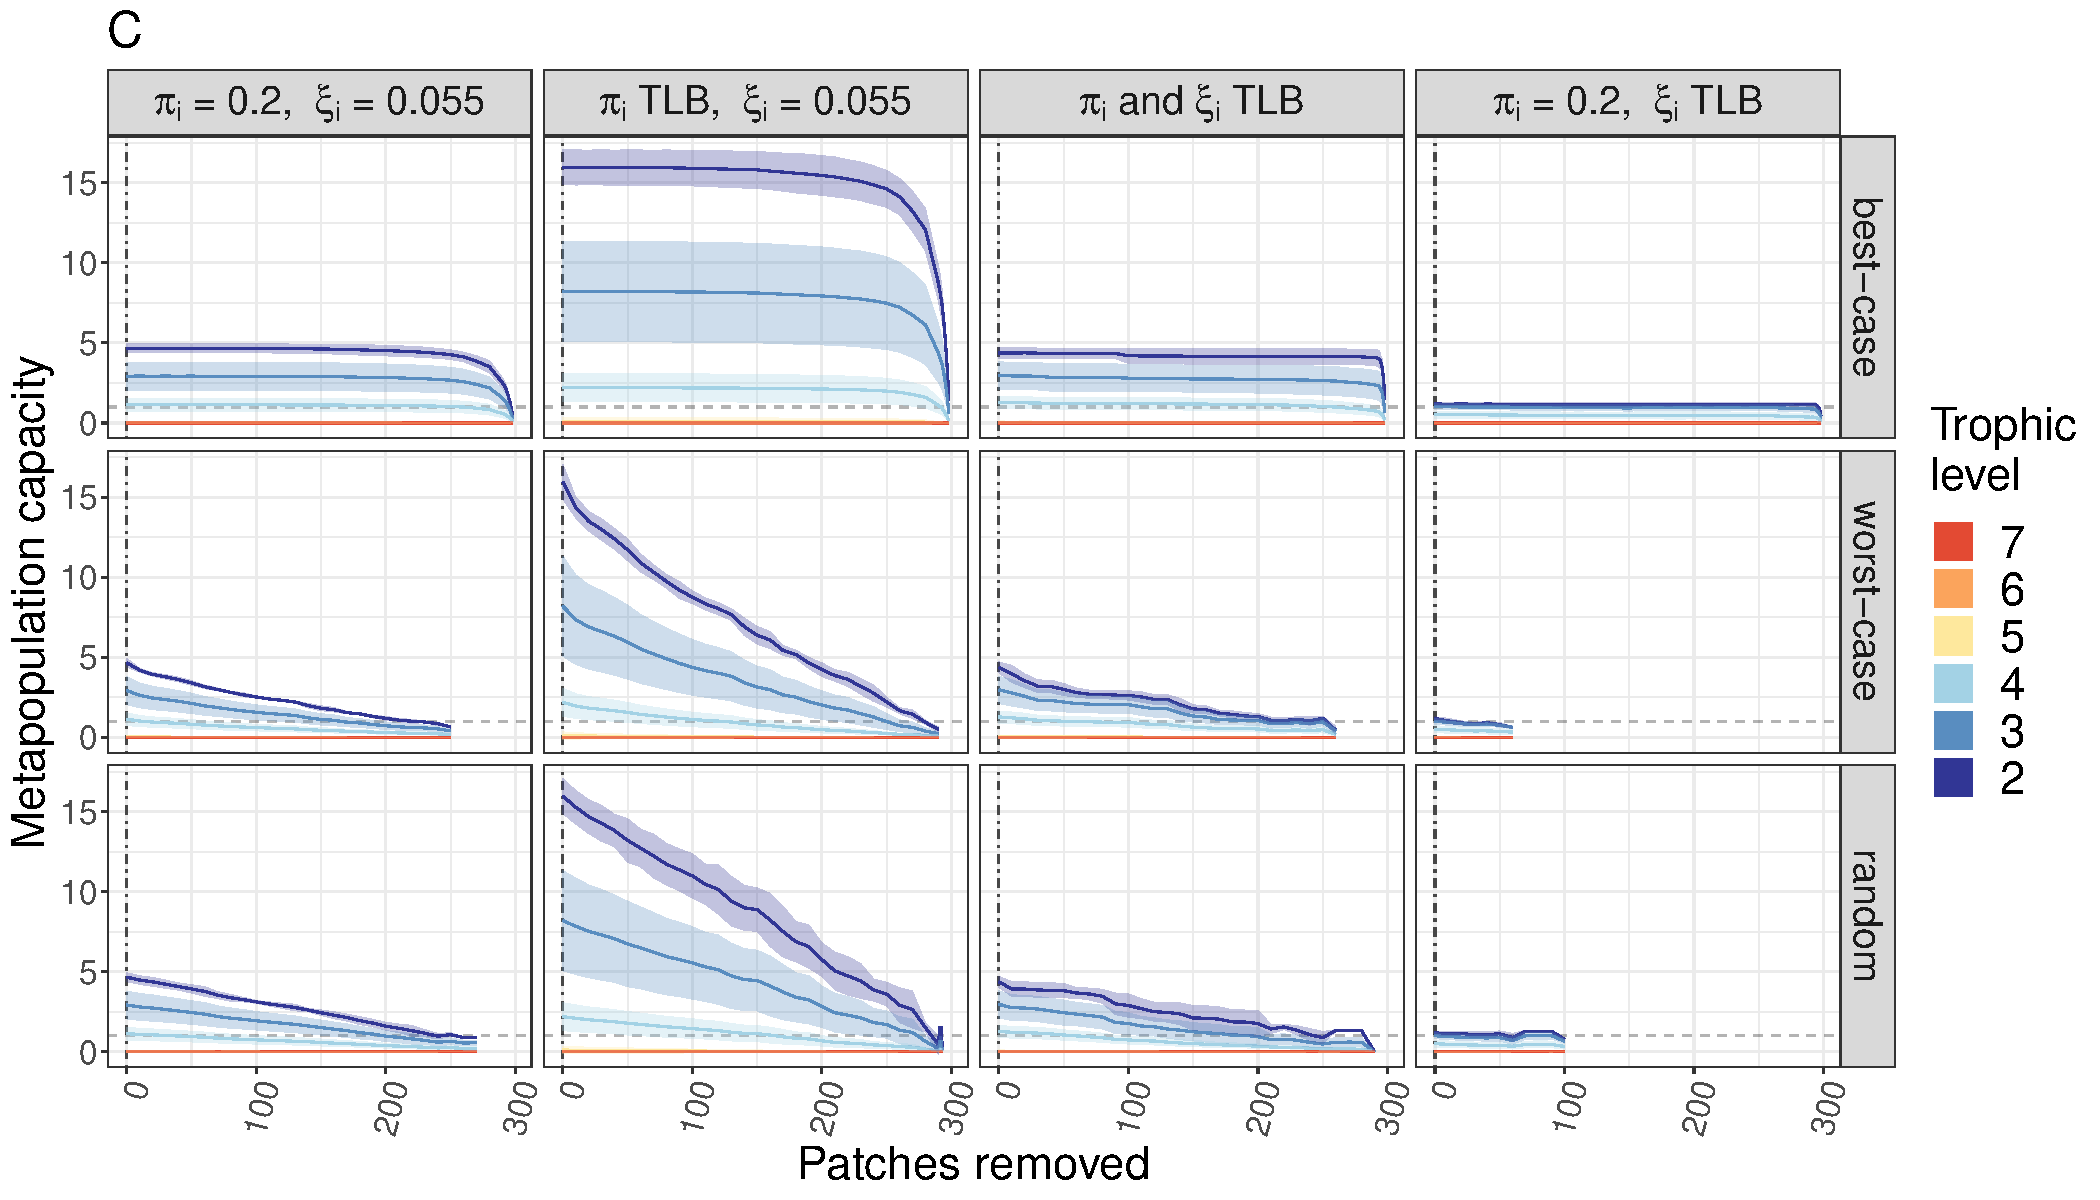
\includegraphics[width=0.8\textwidth,valign=t]{lambda_Weighted_Model_food_web_with_350_consumer_and_50_basal_species_(1)_basal_1_5.pdf}
  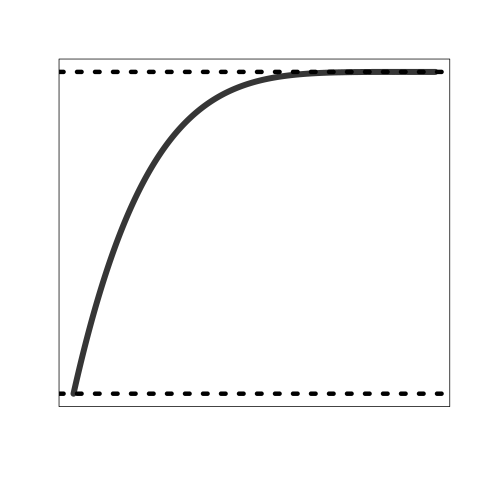
\includegraphics[width=0.19\textwidth,valign=t]{fform_1_5.png}
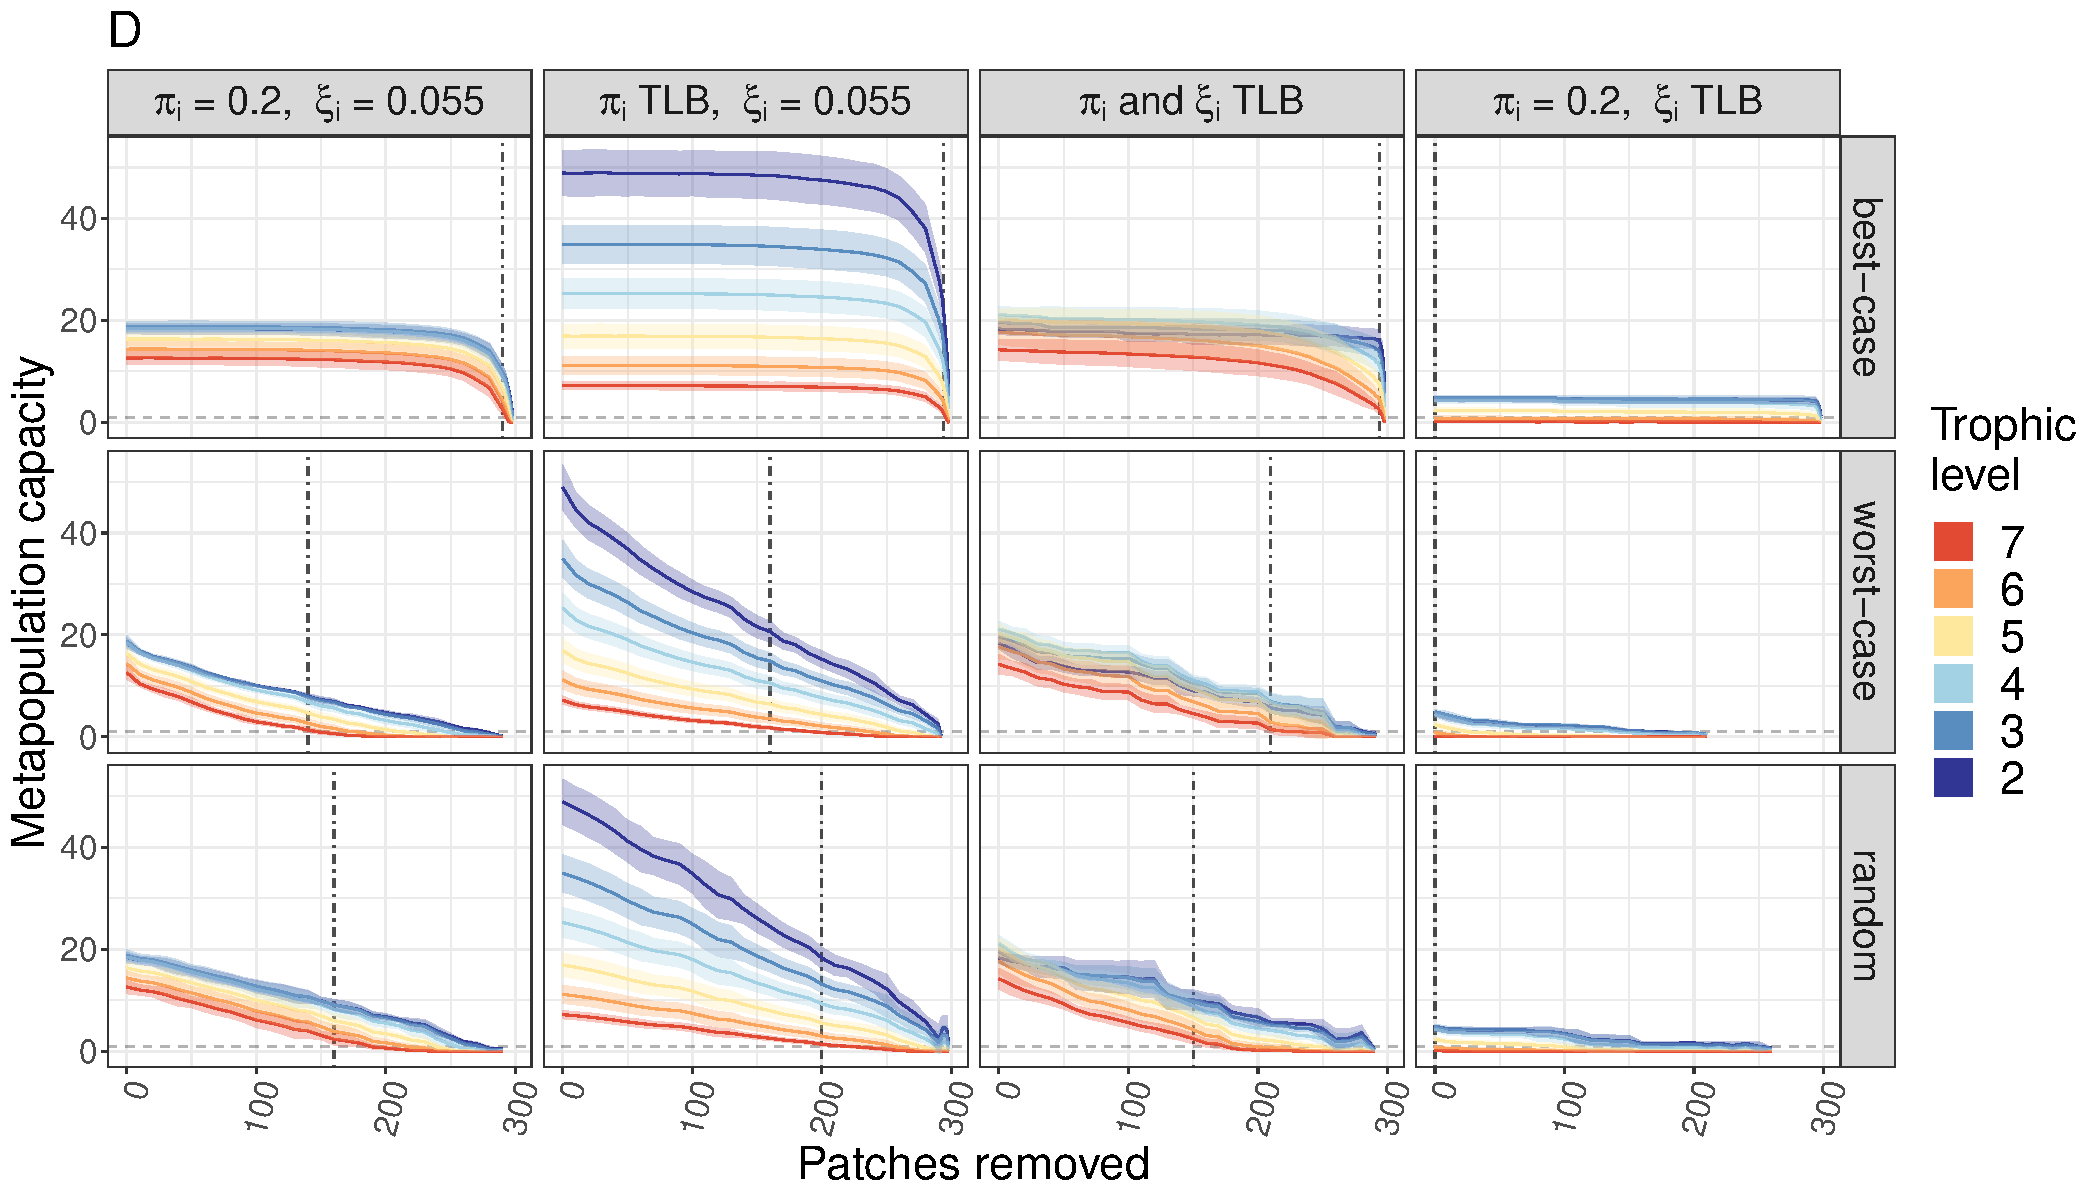
\includegraphics[width=0.8\textwidth,valign=t]{lambda_Weighted_Model_food_web_with_350_consumer_and_50_basal_species_(1)_basal_5_5.pdf}
  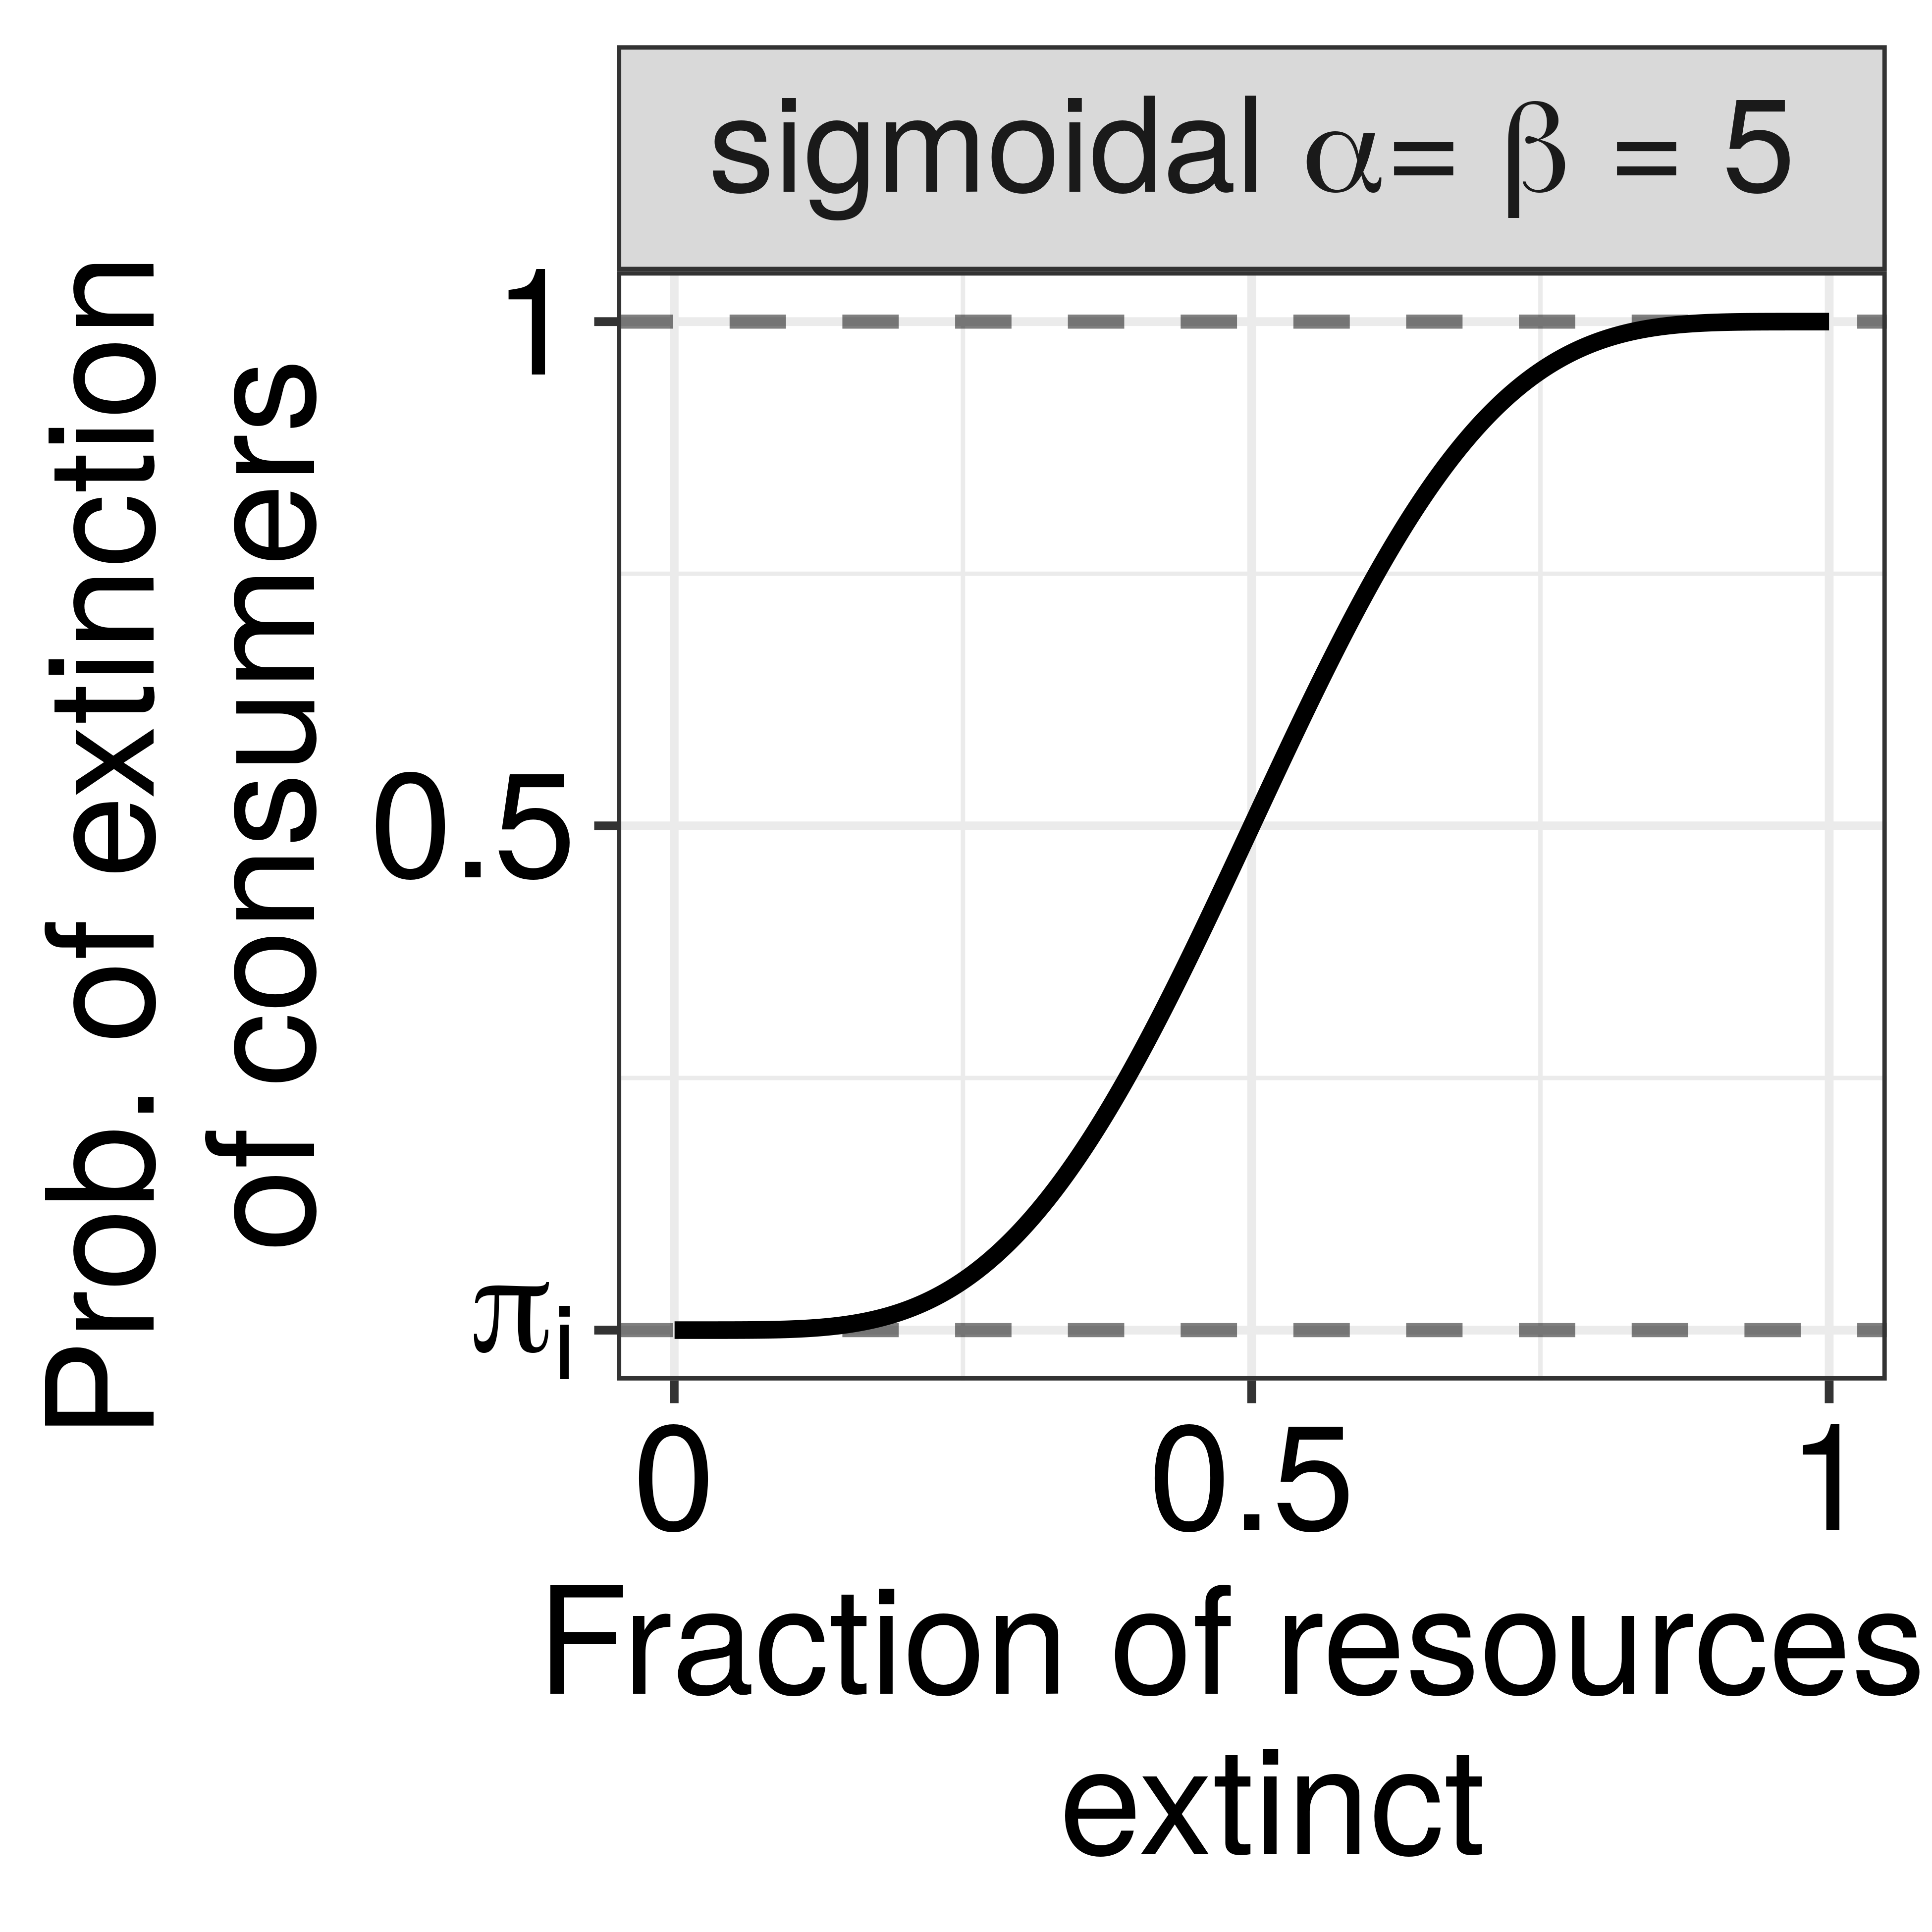
\includegraphics[width=0.19\textwidth,valign=t]{fform_5_5.png}
  \caption{Figure continued.}
 \label{S_fig:patchloss_web1_11_2}
\end{figure}


\section{The maximum number of trophic levels as a function of landscape size and connectivity} \label{sec:ryser}

Based on a fully-fledged dynamical model of spatial food webs, \citet{Ryser2019} estimated the maximum number of trophic levels that can persist given the average patch distance and the number of patches of a landscape. We have re-created their result (which is summarized in Figure~S2 in \citealp{Ryser2019}) using our Bayesian network approach. The results are in Figure~\ref{fig:Ryser_repr}. They are qualitatively unchanged, with the maximum possible trophic level exhibiting a strong dependence of the maximum attainable trophic level on the spatial scale, and a weaker one on the number of patches.

\begin{figure}[!p]
  \centering
  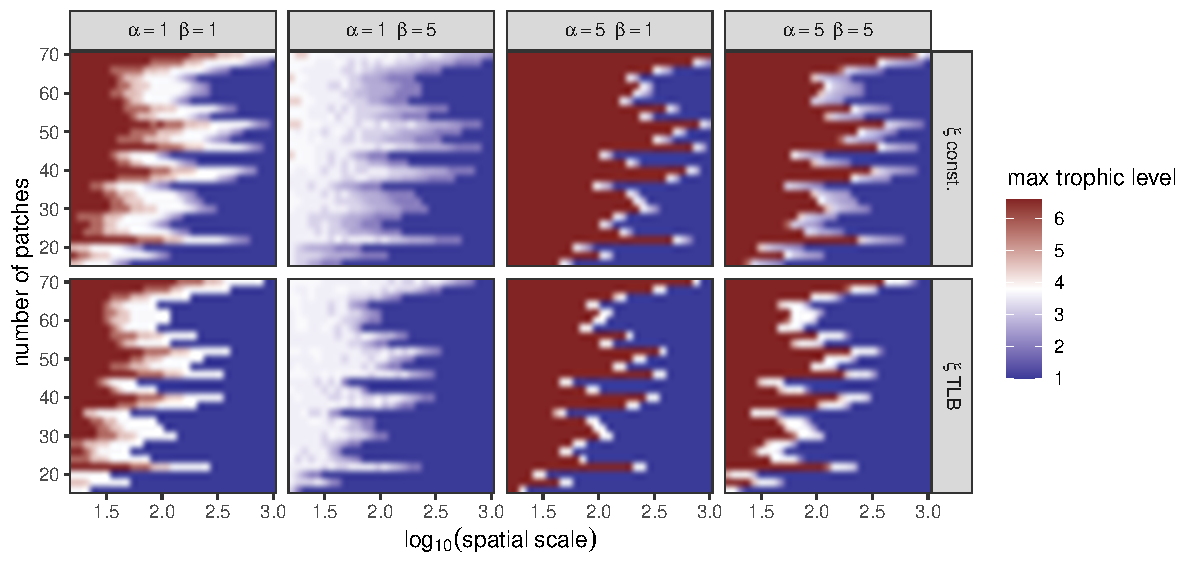
\includegraphics[width=\textwidth]{Ryser_reproduced.pdf}
  \caption{The maximum number of trophic levels (colors) persisting on a landscape with different numbers of patches (ordinate) and average distance between them (abscissa). The web used, which has 50 basal and 350 consumer species, is the same as in Figure~\ref{S_fig:patchloss_350_50_1}. Landscapes were generated just like before, by randomly placing the appropriate number of patches in the unit square. In the top row, each species has an identical dispersal parameter $\xi$ (equal to the spatial scale indicated along the abscissa), while in the bottom row, they were trophic level-based (increasing linearly with trophic level such that their average was equal to the spatial scale parameter). Columns show various parameterizations of the consumer response to prey loss (linear, convex, concave, and sigmoid). The results are qualitatively identical to Figure~S2 in \citet{Ryser2019}: there is a strong dependence of the maximum attainable trophic level on the spatial scale, and a weaker one on the number of patches.}
  \label{fig:Ryser_repr}
\end{figure}

Our approach can even be used to get a deeper, analytical understanding of this result. Approximating trophic networks as trophic chains, assuming a common baseline extinction probability $\pi_i = \pi$, and using the patch-averaging method described in Section~\ref{sec:chain}, we have $T \approx -\lambda_M \log(\pi)$, where $T$ is the maximum number of trophic levels and $\lambda_M$ is the dominant eigenvalue of the dispersal matrix (Eq.~\ref{eq:BN_lambda_chain_20}). Obtaining these eigenvalues for each of the landscapes used in Figure~\ref{fig:Ryser_repr}, we depict this approximation in Figure~\ref{fig:Ryser_semianal}. This figure strongly resembles Figure~S2 in \citet{Ryser2019}, and it is based on the fully tractable approximation $T \approx -\lambda_M \log(\pi)$. This lends further credence to the idea that the pattern observed here and in \citet{Ryser2019} is not contingent on model details, but is a robust logical consequence of combining trophic interactions and metacommunity structure.

\begin{figure}[!p]
  \centering
  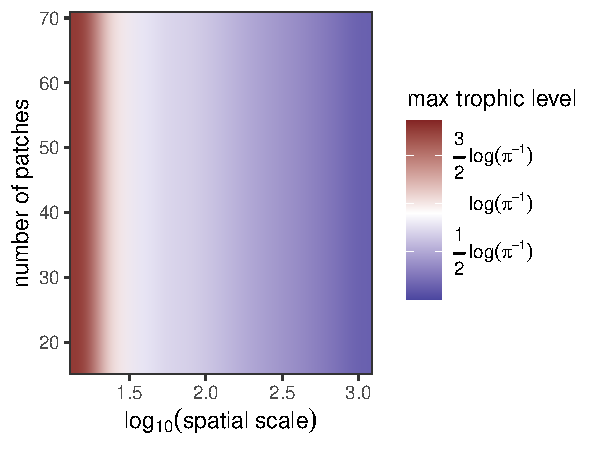
\includegraphics[width=0.62\textwidth]{Ryser_semianalytic.pdf}
  \caption{Analytical approximation of the expected maximum number of trophic levels (colors), given species' dispersal ability (abscissa) and the number of patches in the landscape (ordinate). The heat map is based on the approximation $T \approx \lambda_M \log(\pi^{-1})$ (Eq.~\ref{eq:BN_lambda_chain_20}), with the leading eigenvalues of the landscapes explicitly calculated based on their associated dispersal matrices.}
  \label{fig:Ryser_semianal}
\end{figure}


\section{The effect of removing the links between patches} \label{sec:linkrem}

Instead of removing patches in a given sequence (best-case, worst-case, random), we may do the same with the links connecting those patches. This is tantamount to assuming that, instead of habitat destruction, it is the surrounding matrix that gets eroded or destroyed, making it impossible for individuals to travel between patches. We remove links between pairs of patches, meaning that if the link from patch $A$ to patch $B$ is removed, then so is the link from $B$ to $A$.

To determine the best-case/worst-case link removal sequences, we chose links contributing the least/most to a local change of the basal species' metapopulation capacity. Since this metapopulation capacity is the leading eigenvalue of the matrix $A_i^{kl} = -M_i^{kl} / \log(1 - \delta_i^k)$ (Eq.~\ref{eq:pmjac}), we can apply standard eigenvalue sensitivity analysis to find the links contributing the least/most to the metapopulation capacity \citep[ch.~9]{Caswell2001}. This tells us that
\begin{equation}
  \label{eq:sens_Caswell}
  \frac{\partial \lambda_i}{\partial A_i^{kl}} =
  \frac{v_i^k w_i^l}{\sum_{m=1}^N v_i^m w_i^m} \ ,
\end{equation}
where $\lambda_i$ is the metapopulation capacity of species $i$, $v_i^k$ is the $k$th entry of its corresponding left eigenvector, and $w_i^l$ the $l$th entry of the corresponding right eigenvector. Since the matrix $A_i^{kl}$ has all positive entries, its leading eigenvectors have purely real and positive entries due to the Perron-Frobenius theorem. We numerically determine the right-hand side of Eq.~\ref{eq:sens_Caswell}, and sequentially delete the links corresponding its smallest entries (best-case scenario) or largest entries (worst-case scenario). More precisely, since we are removing links symmetrically, we remove links with the smallest/largest average entry $(v_i^k w_i^l + v_i^l w_i^k)/2$.

Since there are many links in a landscape (with $N$ patches, there are $N(N-1)/2$ links; for $N=300$, we have $44850$ of them), we remove $1500$ links in one iteration, and then re-calculate the sensitivity matrix via Eq.~\ref{eq:sens_Caswell} using the updated matrix $A_i^{kl}$ (from which certain links have already been deleted). The sensitivity formula is only accurate for small perturbations, so removing $1500$ links at a time is somewhat crude but still produces consistent results. As seen in Figure~\ref{S_fig:linkrem}, the results are almost the same as with patch removal, with one important qualitative difference: the random link removal scenario now lies about mid-way between the best- and worst-case ones, instead of being as bad as the worst-case scenario.

\begin{figure}[!p]
  \centering  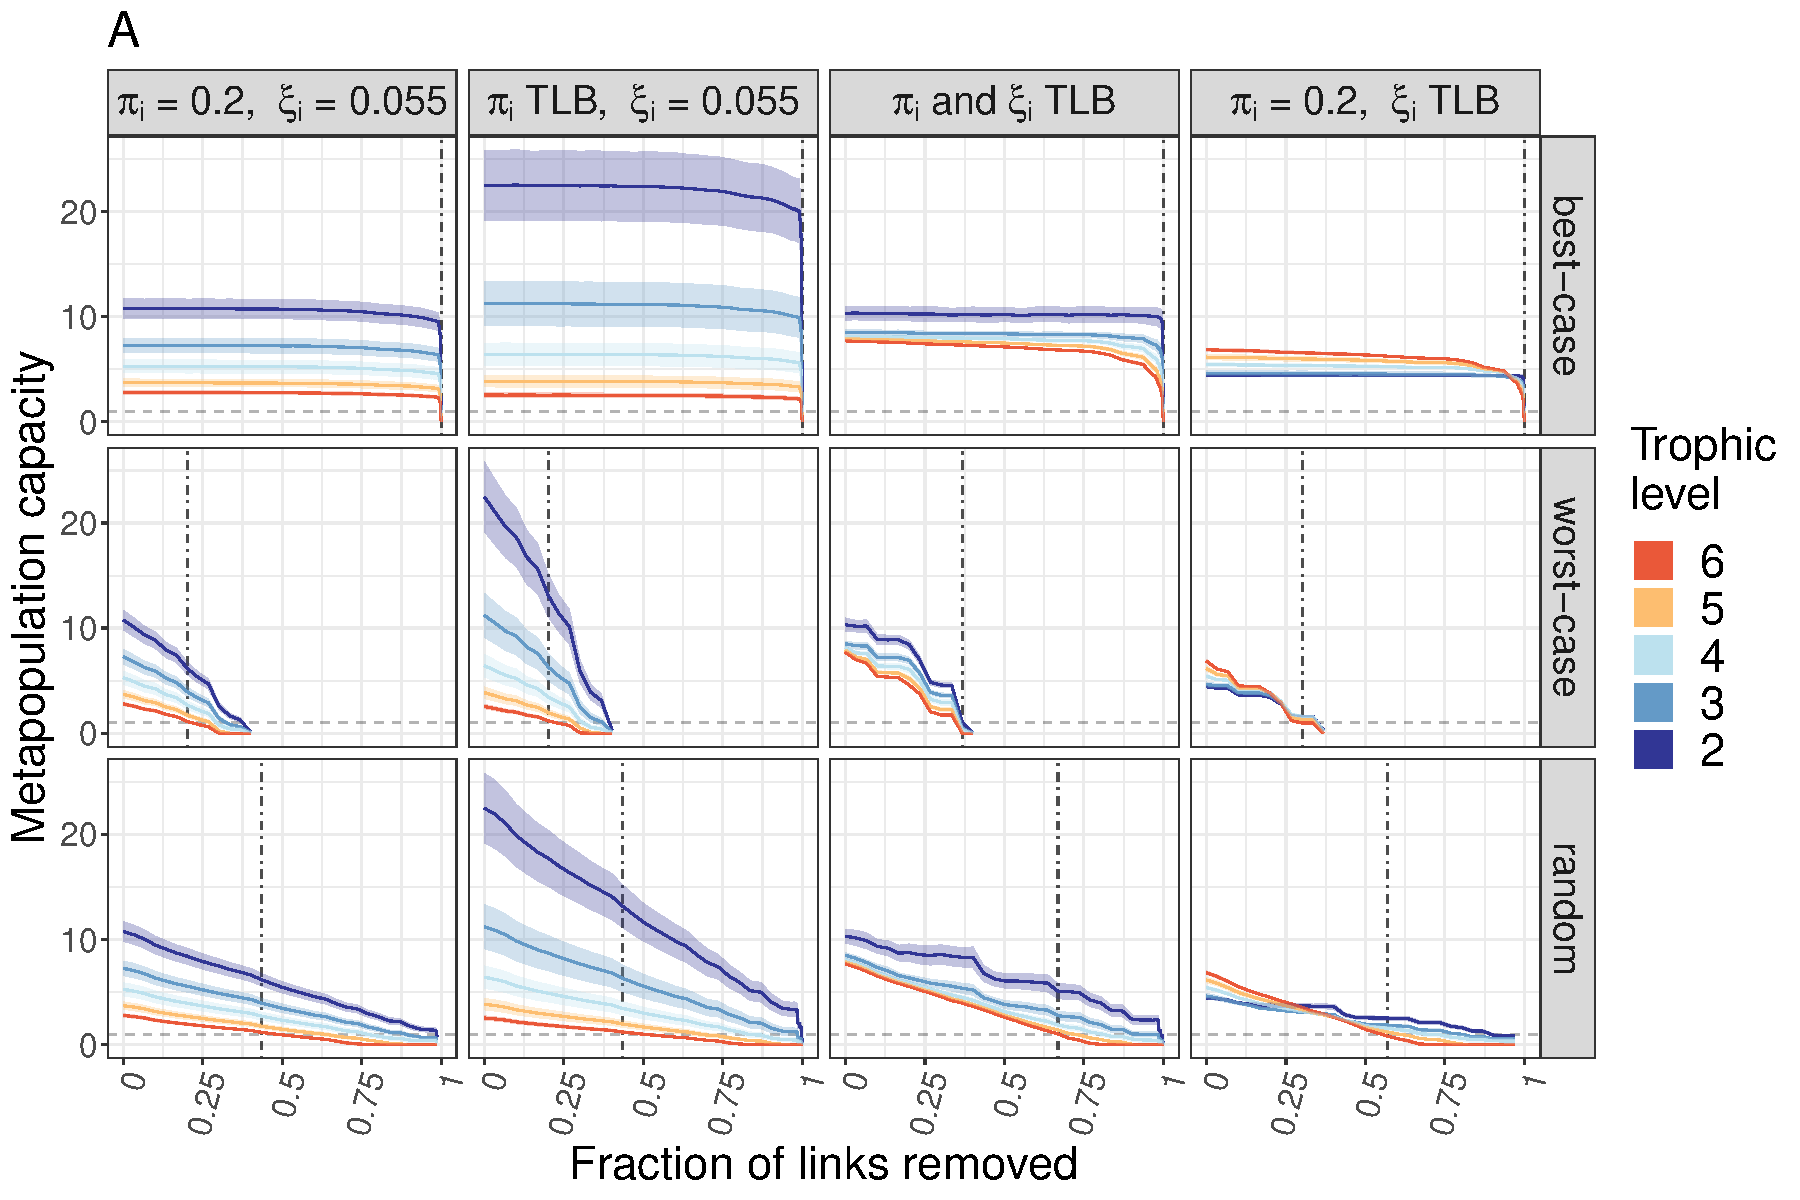
\includegraphics[width=0.8\textwidth,valign=t]{linkrem_Model_food_web_with_300_consumer_and_100_basal_species_basal_1_1_sym.pdf}
  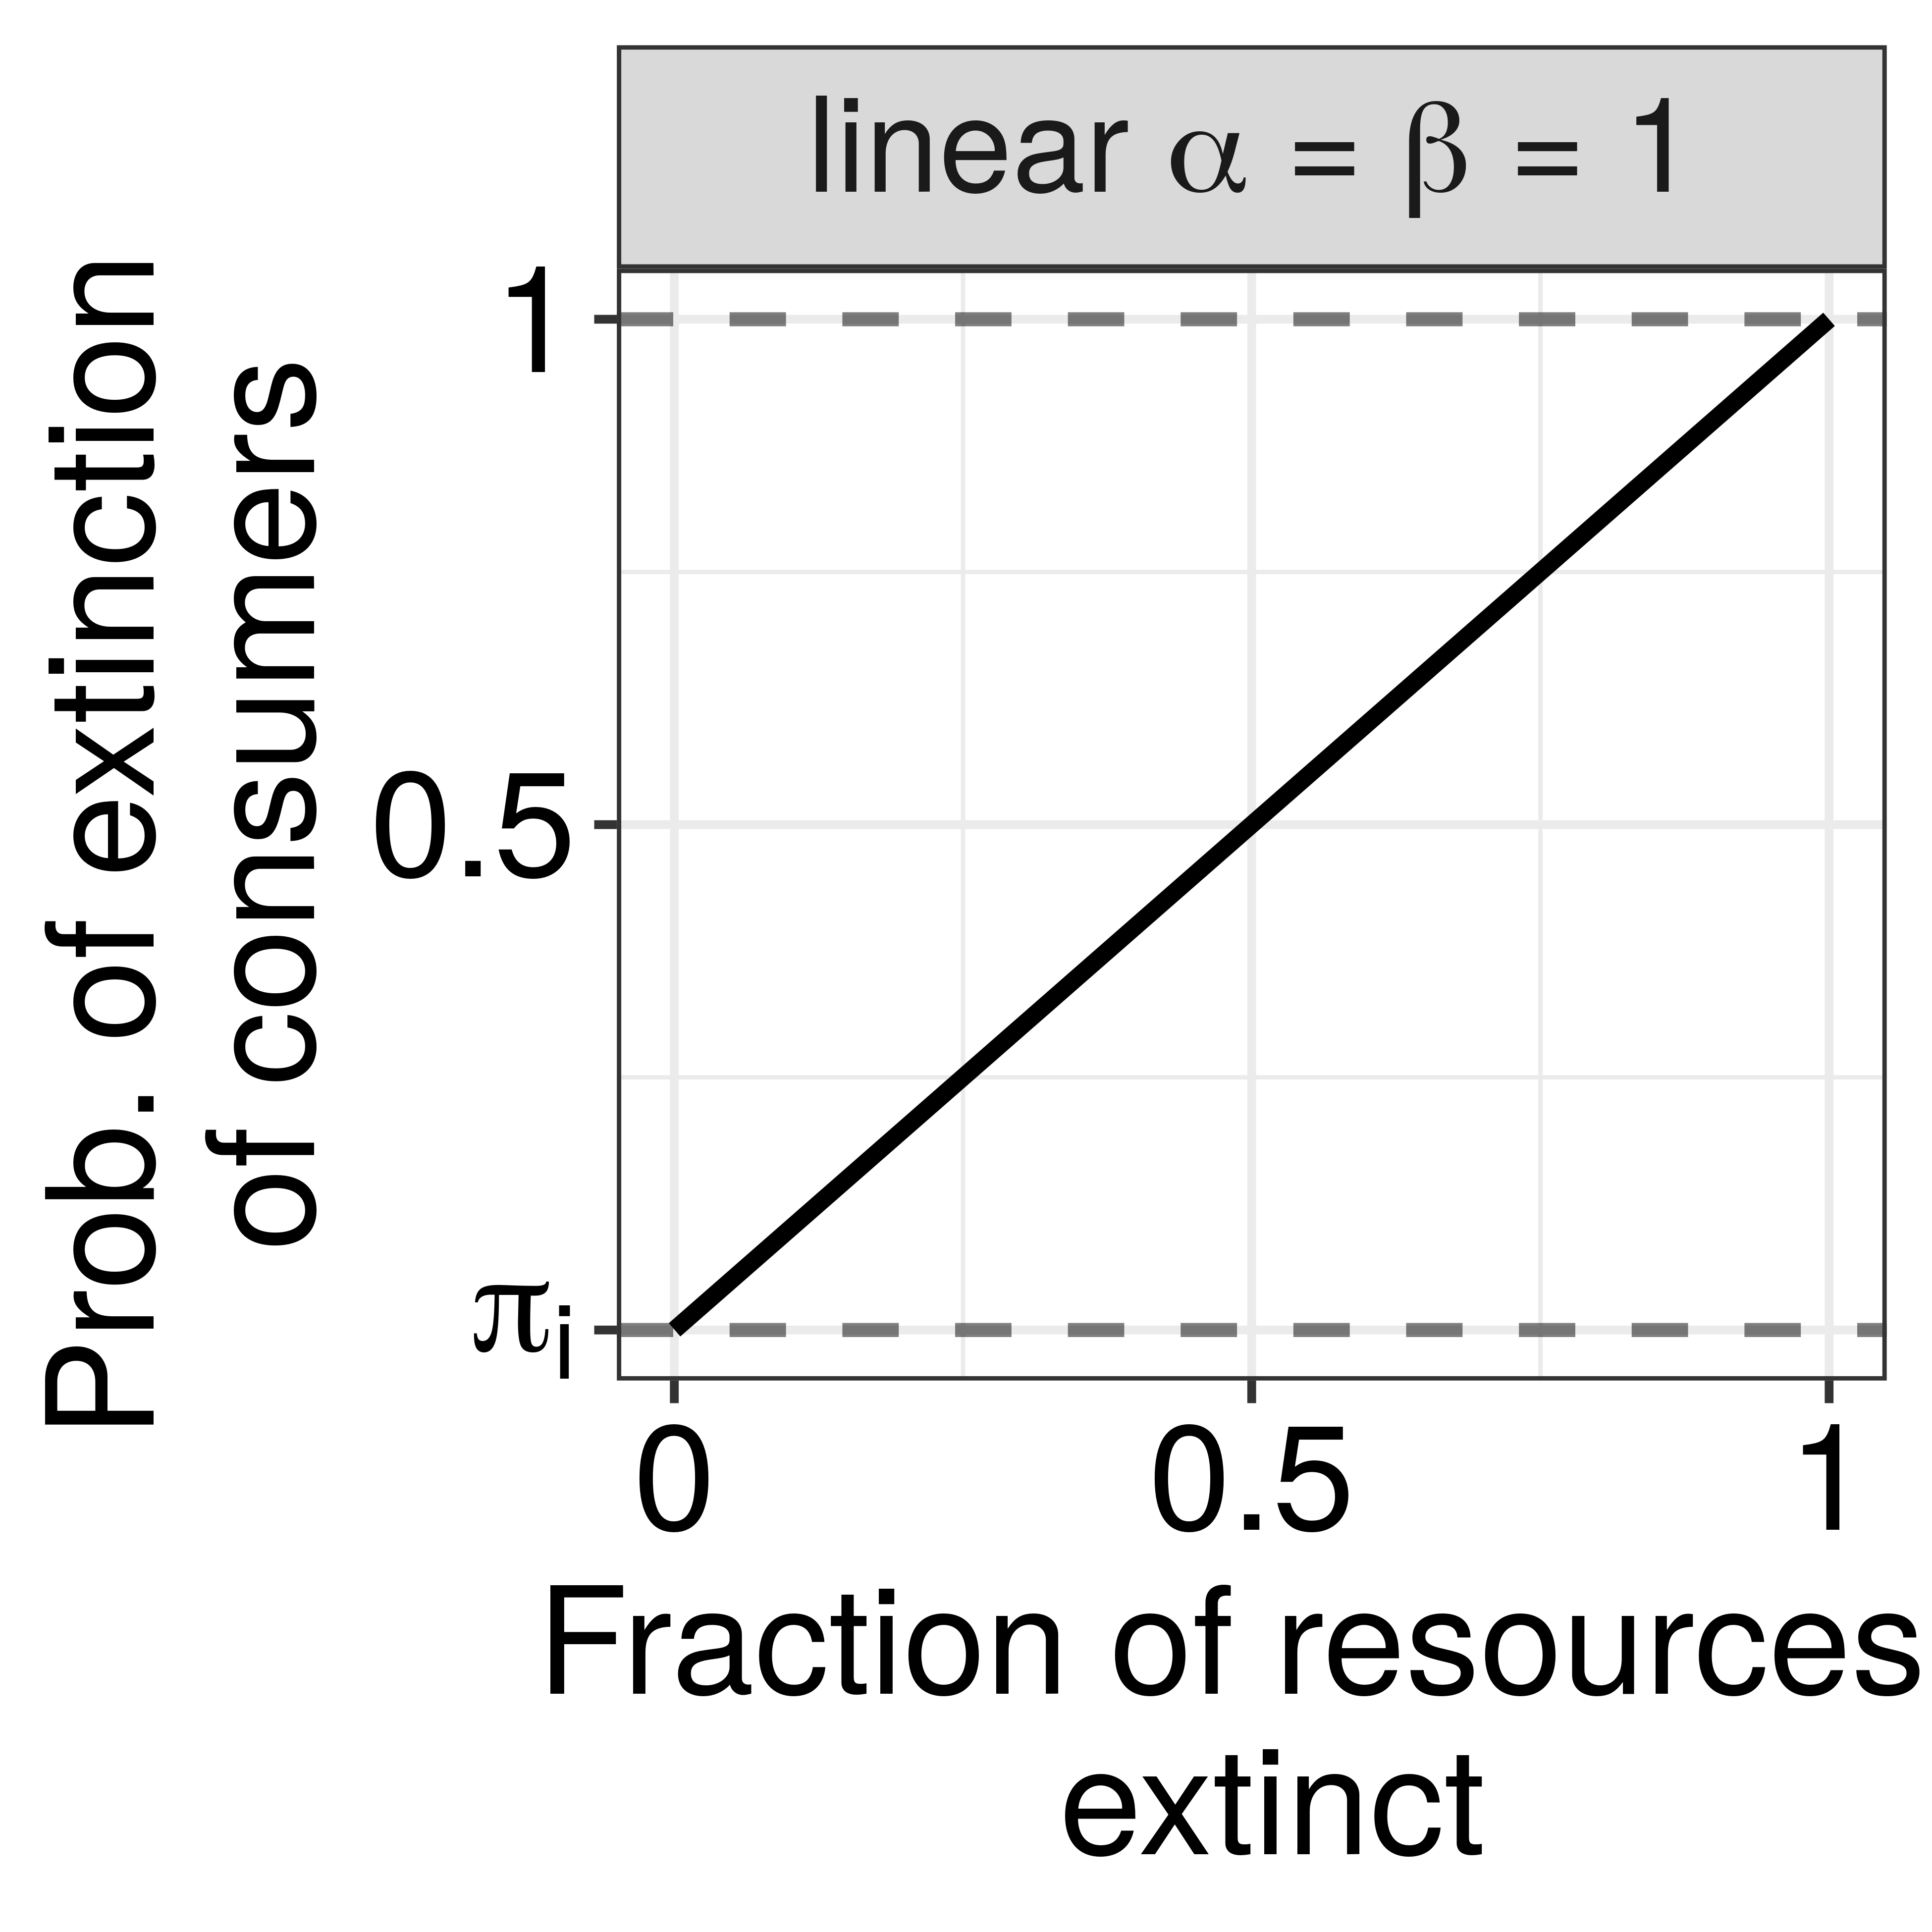
\includegraphics[width=0.19\textwidth,valign=t]{fform_1_1.png}
  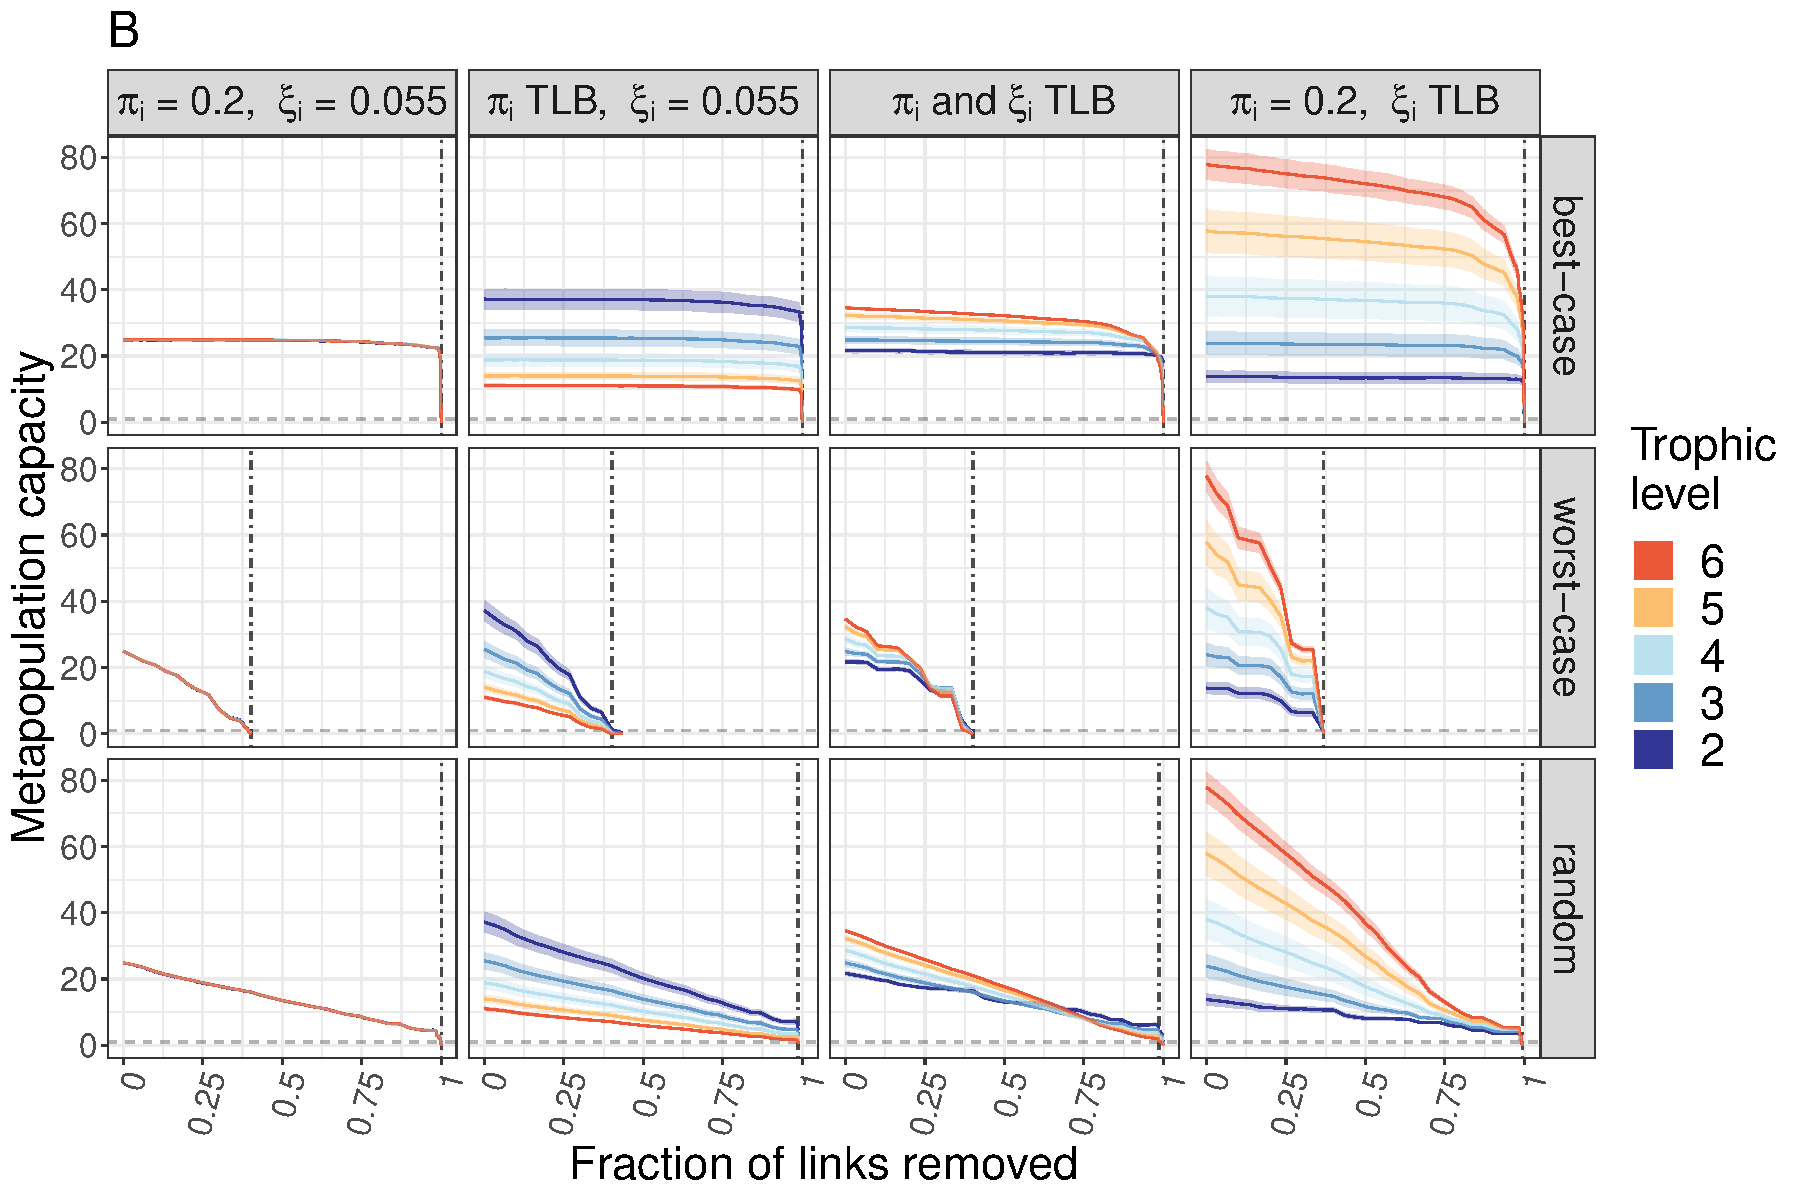
\includegraphics[width=0.8\textwidth,valign=t]{linkrem_Model_food_web_with_300_consumer_and_100_basal_species_basal_5_1_sym.pdf}
  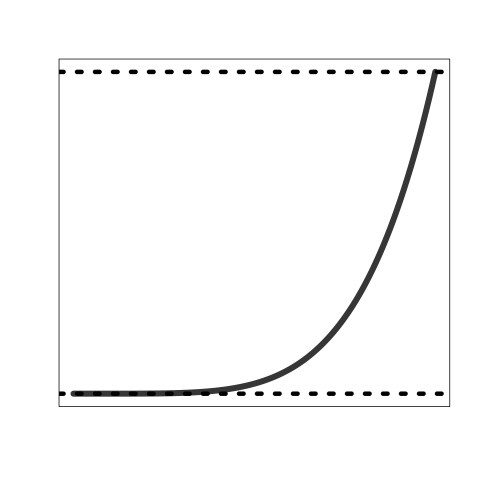
\includegraphics[width=0.19\textwidth,valign=t]{fform_5_1.png}
  \caption{As Figure~2 in the main text, except removing links between pairs of patches, instead of the patches themselves. The abscissa shows the fraction of links removed, out of all possible ones---with $N$ habitat patches, this number is $N(N-1)/2$. Results are very similar to those of patch removal, with one important qualitative difference: the worst-case scenario, instead of being as bad as the worst-case one, is now in between the two extremal scenarios.}
  \label{S_fig:linkrem}
\end{figure}

\begin{figure}[!p]\ContinuedFloat 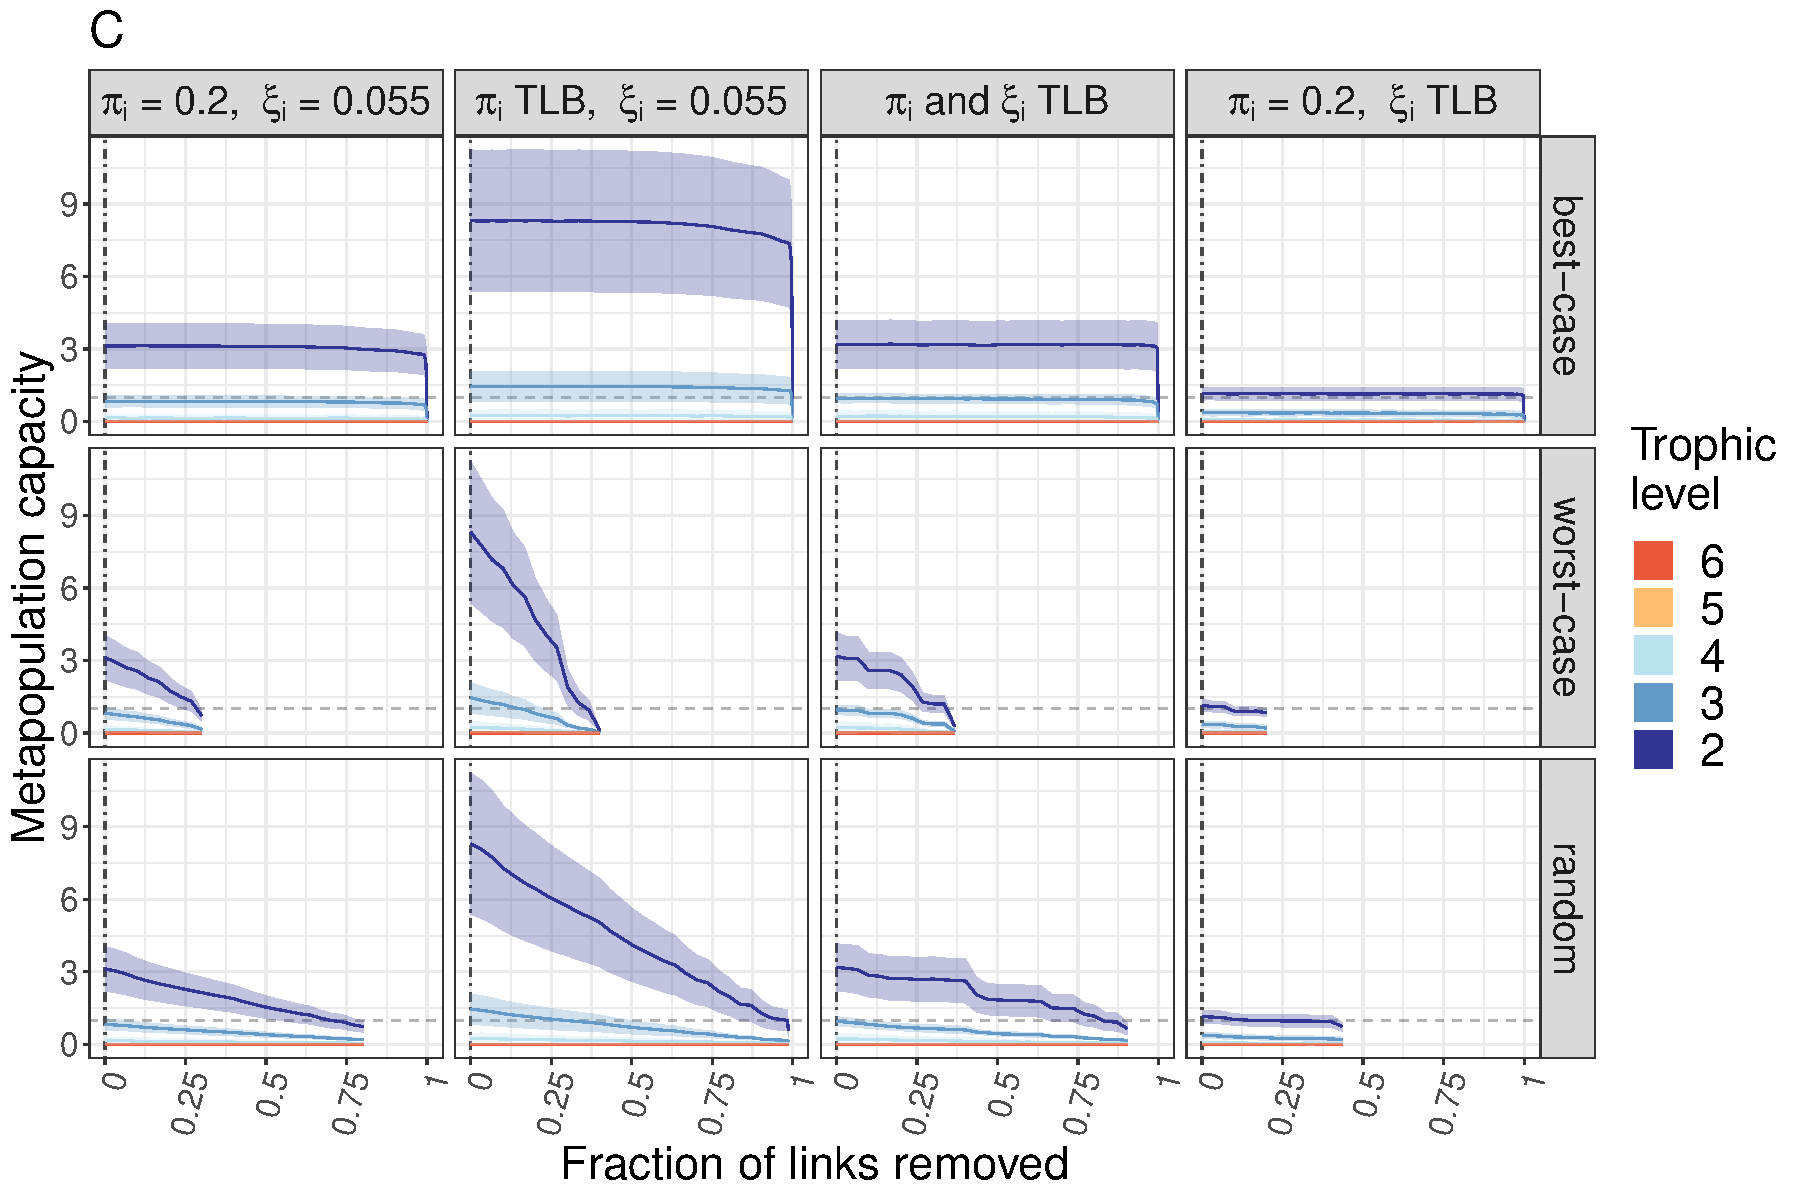
\includegraphics[width=0.8\textwidth,valign=t]{linkrem_Model_food_web_with_300_consumer_and_100_basal_species_basal_1_5_sym.pdf}
  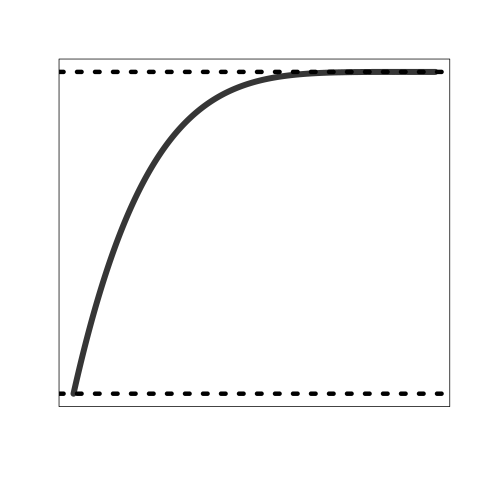
\includegraphics[width=0.19\textwidth,valign=t]{fform_1_5.png}
  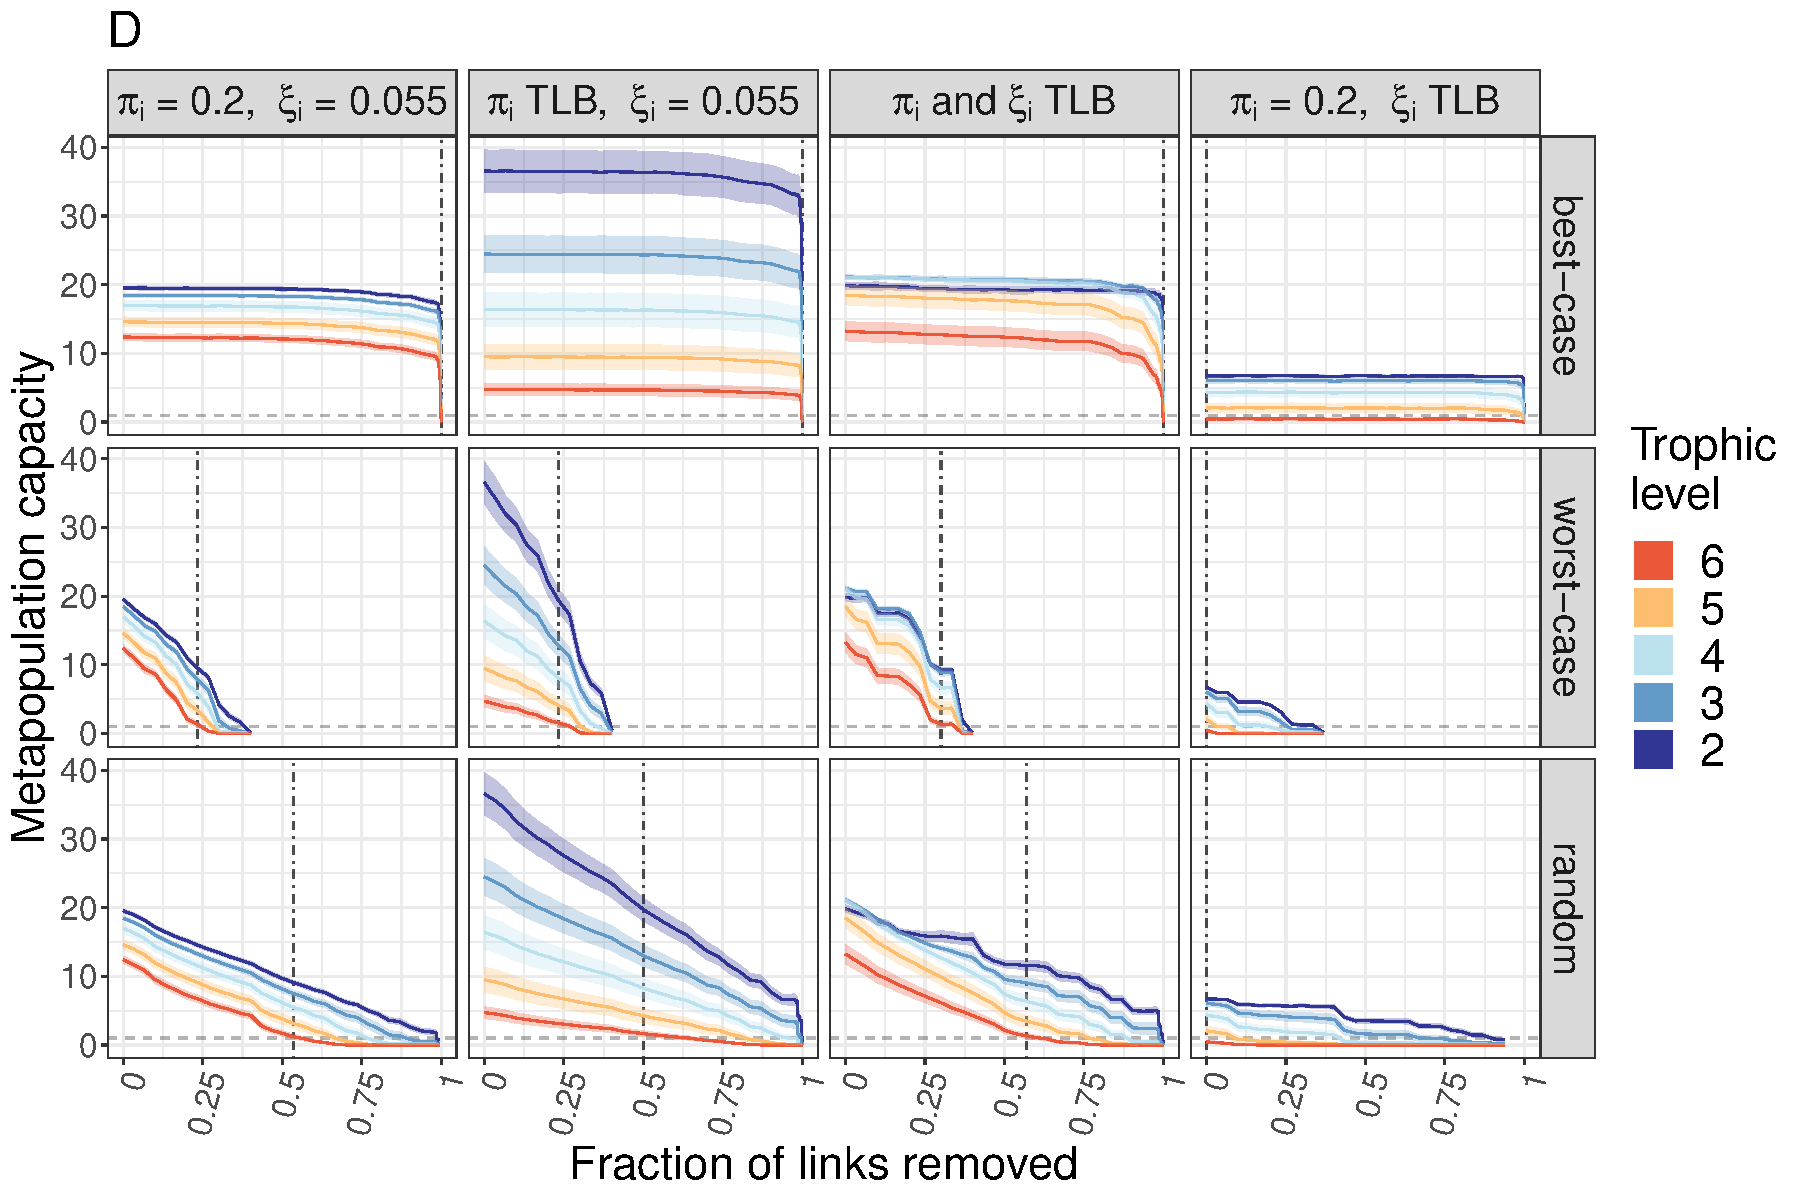
\includegraphics[width=0.8\textwidth,valign=t]{linkrem_Model_food_web_with_300_consumer_and_100_basal_species_basal_5_5_sym.pdf}
  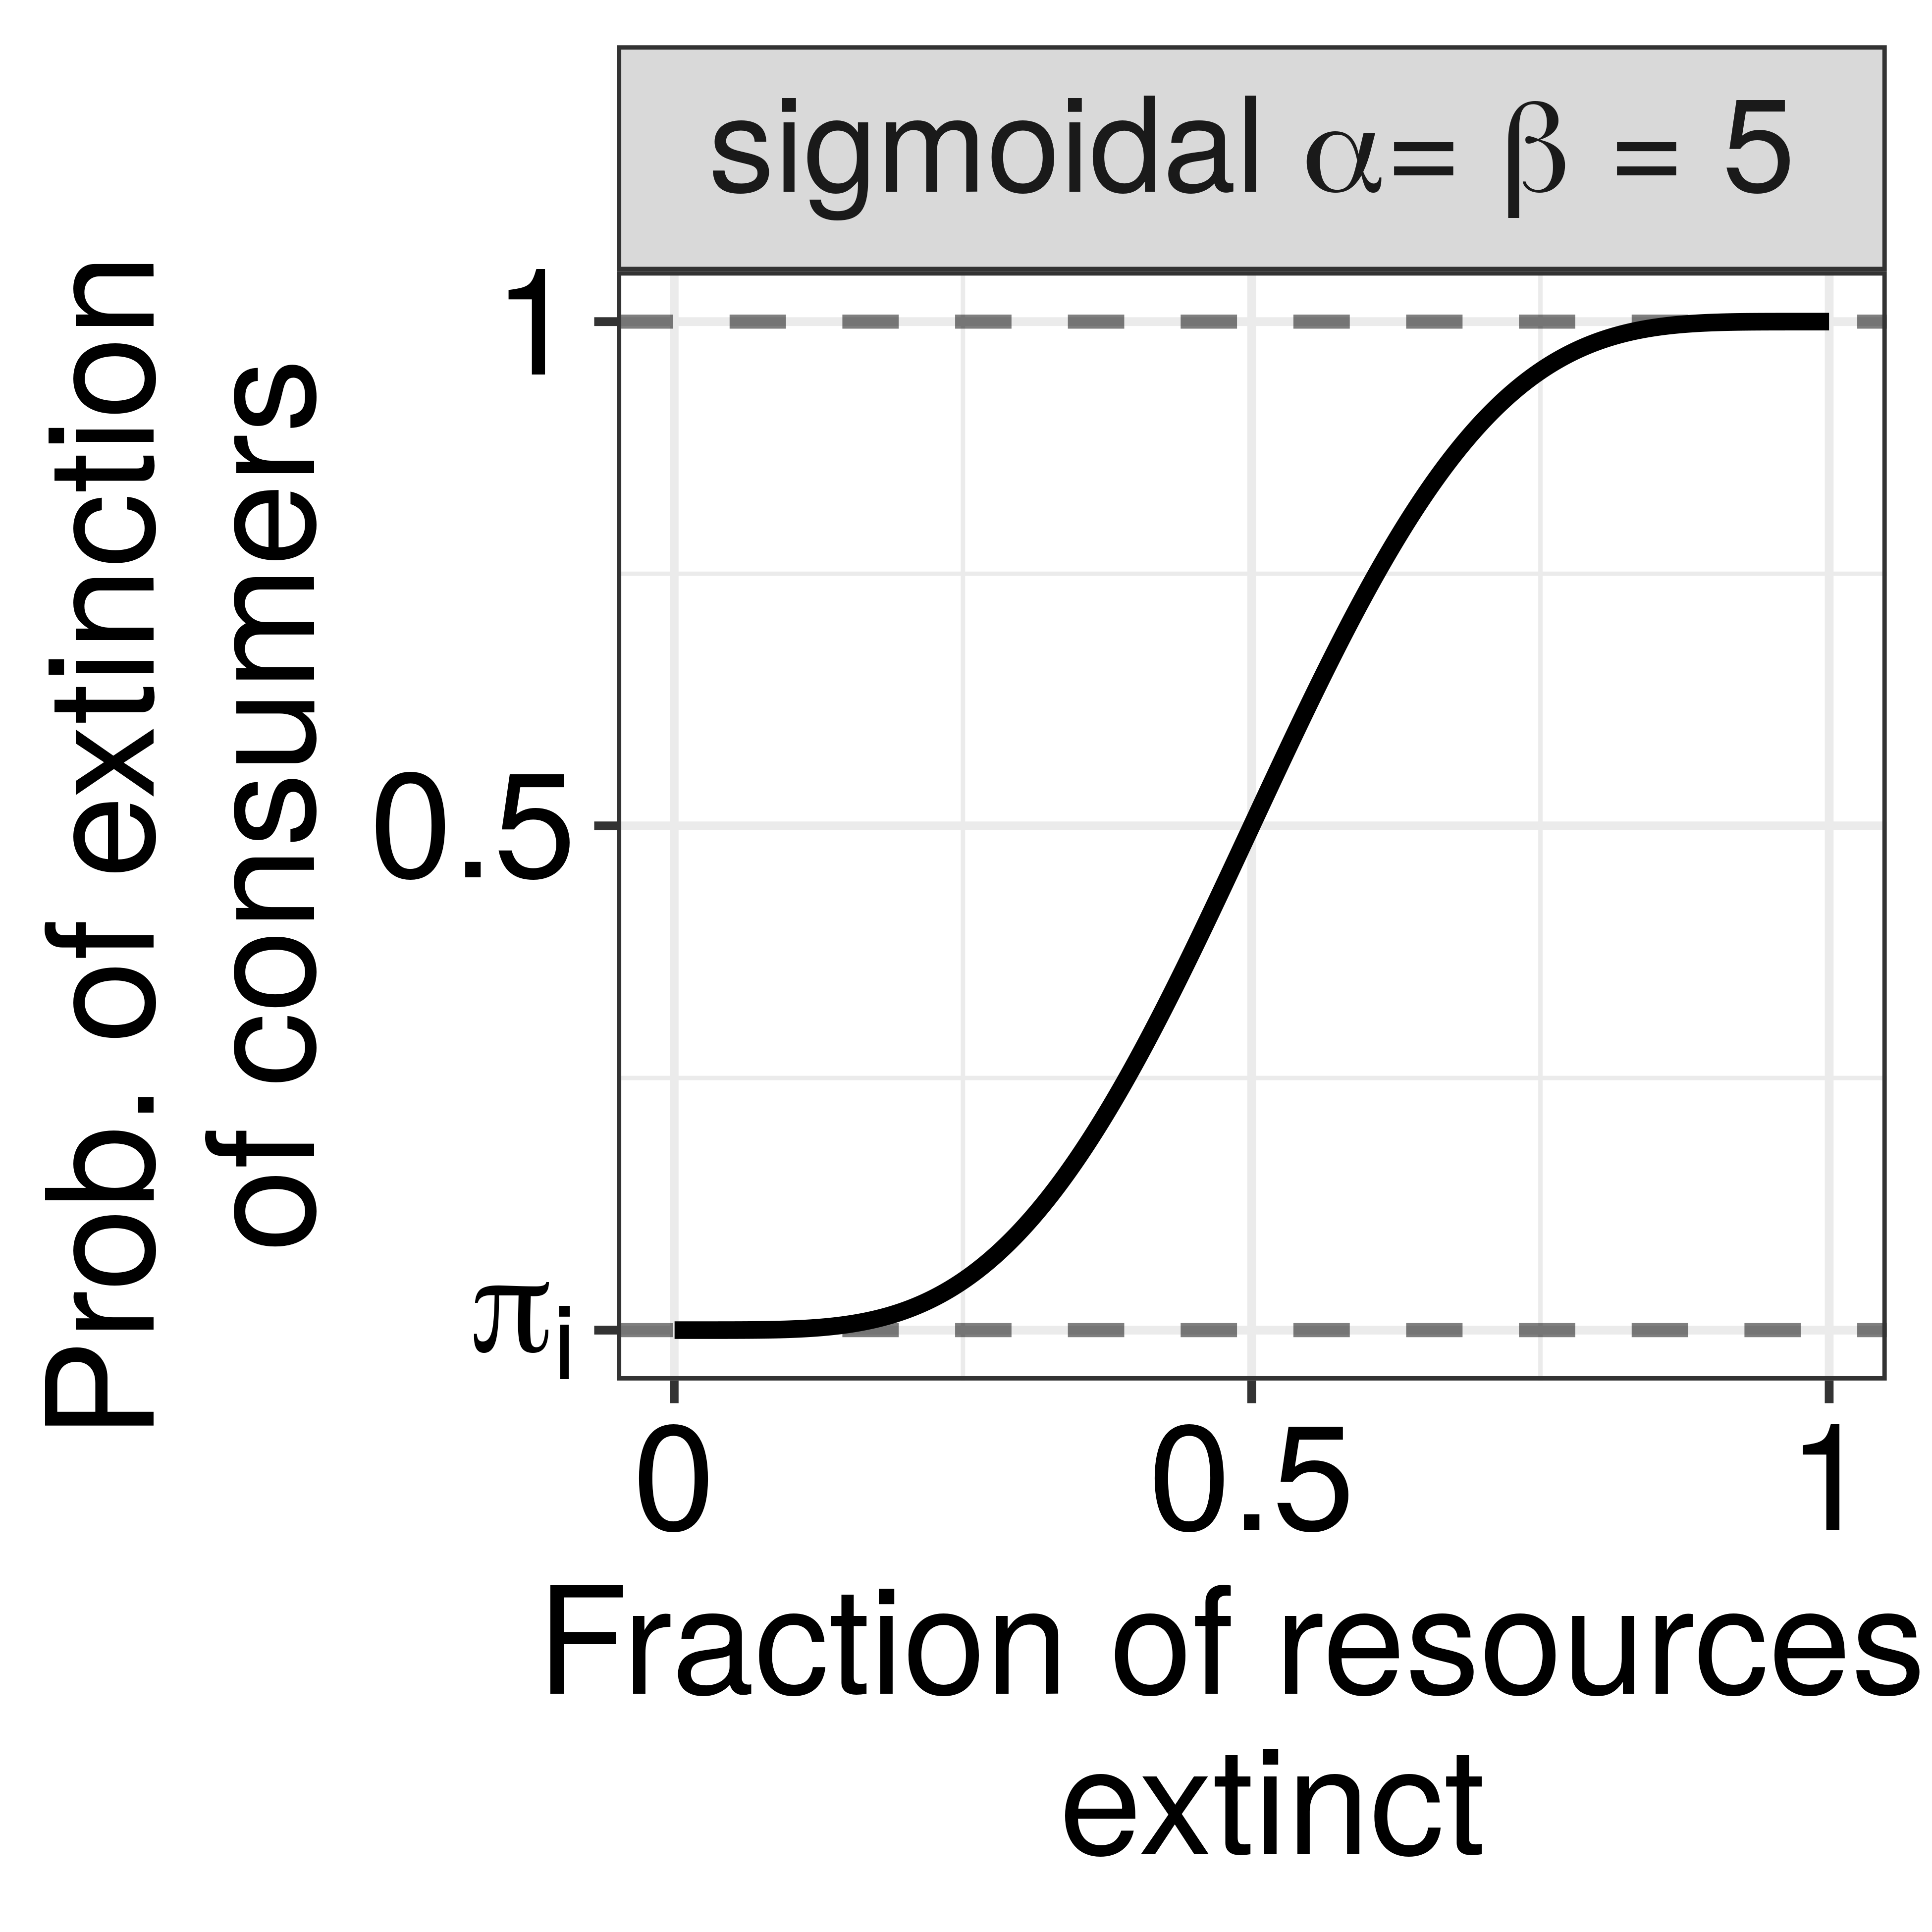
\includegraphics[width=0.19\textwidth,valign=t]{fform_5_5.png}
  \caption{Figure continued.}
  \label{S_fig:linkrem_2}
\end{figure}


\section{Transitioning from a regular grid of habitat patches to random landscapes} \label{sec:gridlike}

Here we highlight the importance of the spatial arrangement of patches across the landscape for our results. Instead of using random landscapes, we create a gradient of landscapes from one in which patches are arranged in a perfect two-dimensional grid, to completely random ones. We do this by creating a $18\times 18$ patch grid, and then jiggling the position of each patch by adding a uniform random value to both their x- and y-coordinates. The range in which the random addition happens ranges from $0$ (perfect grid) to $\pm 0.5$ (perfectly random). Coordinate values over $1$ and below $0$ are wrapped around to appear on the other side of the landscape; e.g., an x-coordinate of $1.2$ is treated as being $0.2$. We then performed the same patch removal analysis as before on each of these landscapes, for the case of $\alpha = \beta = 1$ (linear consumer response to prey loss). We recorded, for each scenario and parameterization, the number of patches that must be removed for the species of a given trophic level to disappear. Results are shown in Figure~\ref{S_fig:gridlike}. In sum, very regular grids of patches lead to more vulnerable species, with fewer patches needing removal to drive them extinct. As the landscapes transition from regular to random patch arrangements, we recover the results observed earlier.

This result demonstrates that landscape arrangement matters, and that highly regular landscapes are more vulnerable than random ones (the same was found by \citealp{Grillietal2015}). The explanation for this is that random landscapes have, by chance, clusters of close-by patches, boosting species' metapopulation capacities. Note though that there are diminishing returns: beyond a point, making  the landscapes even more aggregated no longer enhances persistence, as seen from the figure.

\begin{figure}[!p]
  \centering  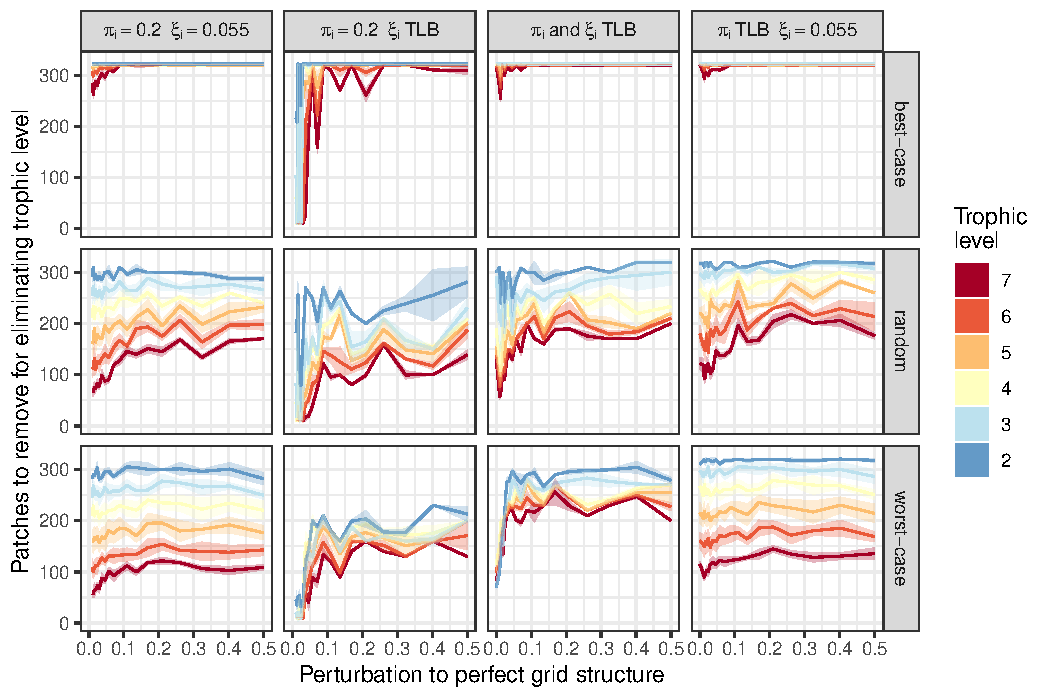
\includegraphics[width=0.95\textwidth,valign=t]{gridlike.pdf}
  \caption{The number of patches (ordinate) which, when removed, cause the extinction of species at various trophic levels (colors, with the lines showing the mean across the species of each trophic level, and the bands around it the one-sigma standard deviations). The abscissa shows how far the patches of the landscape are from being perfectly arranged in a grid ($0$: perfect grid; $0.5$: random landscape). Otherwise, layout is as in Figure~\ref{S_fig:patchloss_350_50_1}. We see that more grid-like landscapes lead to lower persistence thresholds, but that landscapes above a perturbation level of about $0.2$ behave as if they were completely random.}
  \label{S_fig:gridlike}
\end{figure}


\clearpage
\bibliographystyle{elsarticle-harv}
\bibliography{biblio.bib}

\end{document}

